% \documentclass[a4paper,11pt,fleqn]{book}
\documentclass[12pt]{withesis}
\usepackage{physics}
\usepackage{amsmath}
\usepackage[dvipsnames]{xcolor}
% \usepackage{unicode-math}
% \usepackage{amsthm}
% \usepackage{setspace}
\usepackage[font=small,labelfont=bf]{caption}
% \captionsetup[figure]{font=small,labelfont=small}
% \captionsetup[table]{font=small,labelfont=small}
\usepackage[font=small]{subcaption}
\usepackage{amssymb}
\usepackage{tikz}
\usepackage[compat=1.1.0]{tikz-feynman}
\usepackage{head/atlasphysics}
\usepackage{head/ANA-EXOT-2018-64-PAPER-defs}
\usepackage{multirow}
\usepackage{graphicx}
\usepackage{hyperref}
% \usepackage{xcolor}
\usepackage{lipsum}
\usepackage{booktabs}
\usepackage{bm}
\usepackage{dsfont}
\usepackage{nicematrix}
\usepackage{rotating}
% \usepackage{newtxtext,newtxmath}
\usepackage{float}
\definecolor{reddish}{RGB}{155,40,23}
\definecolor{darkgreen}{RGB}{45,74,30}
\definecolor{darkblue}{RGB}{53,76,170}
\usetikzlibrary{quotes}
\usetikzlibrary{shapes,decorations,arrows,calc,arrows.meta,positioning,fit,arrows,shapes.geometric,shapes.multipart,decorations.pathmorphing}

 \usetikzlibrary{decorations.markings, fadings, through}
\usepackage{lineno}
\linenumbers

\newcommand{\graphsage}{\textsc{GraphSAGE}}
\newcommand{\relu}{\textsc{ReLU}}
\newcommand{\ignn}{\textsc{InteractionGNN}}
\newcommand{\bfx}{\mathbf{x}}
\newcommand{\bfm}{\mathbf{m}}
\newcommand{\hssec}{HS06$\times$seconds}
\newcommand{\pu} {\ensuremath{\mu}} 
\newcommand{\epu} {\ensuremath{\expval{\mu}} }



\pagestyle{thesis}
\usepackage[french,german,english]{babel}
\usepackage{algorithm2e}
\RestyleAlgo{ruled}
% %%%%%%%%%%%%%%%%%%%%%%%%%%%%%%%%%%%%%%%%%%%%%%
%
%		Thesis Settings
%
%		EDOC Template
%		2011
%
%%%%%%%%%%%%%%%%%%%%%%%%%%%%%%%%%%%%%%%%%%%%%%


\usepackage[T1]{fontenc}
\usepackage[utf8]{inputenc}
\usepackage[french,german,english]{babel}
\usepackage{algorithm2e}
\RestyleAlgo{ruled}

%%%%%%%%%%%%%%%%%%%%%%%%%%%%%%%%%%%%%%%%%%%%%%%
%% EDOC THESIS TEMPLATE: Variant 1.0 -> Latin modern, large text width&height
%%%%%%%%%%%%%%%%%%%%%%%%%%%%%%%%%%%%%%%%%%%%%%%
%\usepackage{lmodern}
%\usepackage[a4paper,top=22mm,bottom=28mm,inner=35mm,outer=25mm]{geometry}
%%%%%%%%%%%%%%%%%%%%%%%%%%%%%%%%%%%%%%%%%%%%%%%

%%%%%%%%%%%%%%%%%%%%%%%%%%%%%%%%%%%%%%%%%%%%%%
% EDOC THESIS TEMPLATE: Variant 2.0 -> Utopia, Gabarrit A (lighter pages)
%%%%%%%%%%%%%%%%%%%%%%%%%%%%%%%%%%%%%%%%%%%%%%
\usepackage{fourier} % Utopia font-typesetting including mathematical formula compatible with newer TeX-Distributions (>2010)
%\usepackage{utopia} % on older systems -> use this package instead of fourier in combination with mathdesign for better looking results
%\usepackage[adobe-utopia]{mathdesign}
\DeclareMathAlphabet{\mathcal}{OMS}{cmsy}{m}{n}
\setlength{\textwidth}{146.8mm} % = 210mm - 37mm - 26.2mm
\setlength{\oddsidemargin}{11.6mm} % 37mm - 1in (from hoffset)
\setlength{\evensidemargin}{0.8mm} % = 26.2mm - 1in (from hoffset)
\setlength{\topmargin}{-2.2mm} % = 0mm -1in + 23.2mm 
\setlength{\textheight}{221.9mm} % = 297mm -29.5mm -31.6mm - 14mm (12 to accomodate footline with pagenumber)
\setlength{\headheight}{14pt}
%%%%%%%%%%%%%%%%%%%%%%%%%%%%%%%%%%%%%%%%%%%%%%



\setlength{\parindent}{0pt}

\usepackage{setspace} % increase interline spacing slightly
\setstretch{1.2}

\makeatletter
\setlength{\@fptop}{0pt}  % for aligning all floating figures/tables etc... to the top margin
\makeatother


\usepackage{graphicx,xcolor}
\graphicspath{{images/}}

\usepackage{subfig}
\usepackage{booktabs}
\usepackage{lipsum}
\usepackage{microtype}
\usepackage{url}
\usepackage[final]{pdfpages}

\usepackage{fancyhdr}
\renewcommand{\sectionmark}[1]{\markright{\thesection\ #1}}
\pagestyle{fancy}
	\fancyhf{}
	\renewcommand{\headrulewidth}{0.4pt}
	\renewcommand{\footrulewidth}{0pt}
	\fancyhead[OR]{\bfseries \nouppercase{\rightmark}}
	\fancyhead[EL]{\bfseries \nouppercase{\leftmark}}
% 	\fancyfoot[EL,OR]{\thepage}
    \fancyfoot[R]{\thepage}
\fancypagestyle{plain}{
	\fancyhf{}
	\renewcommand{\headrulewidth}{0pt}
	\renewcommand{\footrulewidth}{0pt}
% 	\fancyfoot[EL,OR]{\thepage}
	\fancyfoot[R]{\thepage}
	}
\fancypagestyle{addpagenumbersforpdfimports}{
	\fancyhead{}
	\renewcommand{\headrulewidth}{0pt}
	\fancyfoot{}
% 	\fancyfoot[RO,LE]{\thepage}
    \fancyfoot[R]{\thepage}
}

\usepackage{listings}
\lstset{language=[LaTeX]Tex,tabsize=4, basicstyle=\scriptsize\ttfamily, showstringspaces=false, numbers=left, numberstyle=\tiny, numbersep=10pt, breaklines=true, breakautoindent=true, breakindent=10pt}

\usepackage{hyperref}
\hypersetup{pdfborder={0 0 0},
	colorlinks=true,
	linkcolor=blue,
	citecolor=red,
	urlcolor=blue}
\urlstyle{same}

\makeatletter
\def\cleardoublepage{\clearpage\if@twoside \ifodd\c@page\else
    \hbox{}
    \thispagestyle{empty}
    \newpage
    \if@twocolumn\hbox{}\newpage\fi\fi\fi}
\makeatother \clearpage{\pagestyle{plain}\cleardoublepage}


%%%%% CHAPTER HEADER %%%%
\usepackage{color}
\usepackage{tikz}
\usepackage[explicit]{titlesec}
\newcommand*\chapterlabel{}
%\renewcommand{\thechapter}{\Roman{chapter}}
\titleformat{\chapter}[display]  % type (section,chapter,etc...) to vary,  shape (eg display-type)
	{\normalfont\bfseries\Huge} % format of the chapter
	{\gdef\chapterlabel{\thechapter\ }}     % the label 
 	{0pt} % separation between label and chapter-title
 	  {\begin{tikzpicture}[remember picture,overlay]
    \node[yshift=-8cm] at (current page.north west)
      {\begin{tikzpicture}[remember picture, overlay]
        \draw[fill=black] (0,0) rectangle(35.5mm,15mm);
        \node[anchor=north east,yshift=-7.2cm,xshift=34mm,minimum height=30mm,inner sep=0mm] at (current page.north west)
        {\parbox[top][30mm][t]{15mm}{\raggedleft $\phantom{\textrm{l}}$\color{white}\chapterlabel}};  %the black l is just to get better base-line alingement
        \node[anchor=north west,yshift=-7.2cm,xshift=37mm,text width=\textwidth,minimum height=30mm,inner sep=0mm] at (current page.north west)
              {\parbox[top][30mm][t]{\textwidth}{\color{black}#1}};
       \end{tikzpicture}
      };
   \end{tikzpicture}
   \gdef\chapterlabel{}
  } % code before the title body

\titlespacing*{\chapter}{0pt}{50pt}{30pt}
\titlespacing*{\section}{0pt}{13.2pt}{*0}  % 13.2pt is line spacing for a text with 11pt font size
\titlespacing*{\subsection}{0pt}{13.2pt}{*0}
\titlespacing*{\subsubsection}{0pt}{13.2pt}{*0}

\newcounter{myparts}
\newcommand*\partlabel{}
\titleformat{\part}[display]  % type (section,chapter,etc...) to vary,  shape (eg display-type)
	{\normalfont\bfseries\Huge} % format of the part
	{\gdef\partlabel{\thepart\ }}     % the label 
 	{20pt} % separation between label and part-title
 	  {\setlength{\unitlength}{20mm}
	  \addtocounter{myparts}{1}
	  \begin{tikzpicture}[remember picture,overlay]
    \node[anchor=north west,xshift=-65mm,yshift=-6.9cm-\value{myparts}*20mm] at (current page.north east) % for unknown reasons: 3mm missing -> 65 instead of 62
      {\begin{tikzpicture}[remember picture, overlay]
        \draw[fill=black] (0,0) rectangle(62mm,20mm);   % -\value{myparts}\unitlength
        \node[anchor=north west,yshift=-6.1cm-\value{myparts}*20mm,xshift=-60.5mm,minimum height=30mm,inner sep=0mm] at (current page.north east)
        {\parbox[top][30mm][t]{55mm}{\raggedright \color{white}Part \partlabel $\phantom{\textrm{l}}$}};  %the phantom l is just to get better base-line alingement
        \node[anchor=north east,yshift=-6.1cm-\value{myparts}*20mm,xshift=-63.5mm,text width=0.9\textwidth,minimum height=30mm,inner sep=0mm] at (current page.north east)
              {\parbox[top][30mm][t]{\textwidth}{\raggedleft \color{black}#1}};
       \end{tikzpicture}
      };
   \end{tikzpicture}
   \gdef\partlabel{}
  } % code before the title body

\usepackage{amsmath}
% Fix the problem with delimiter size caused by fourier and amsmath packages.
\makeatletter
\def\resetMathstrut@{%
  \setbox\z@\hbox{%
    \mathchardef\@tempa\mathcode`\(\relax
      \def\@tempb##1"##2##3{\the\textfont"##3\char"}%
      \expandafter\@tempb\meaning\@tempa \relax
  }%
  \ht\Mathstrutbox@1.2\ht\z@ \dp\Mathstrutbox@1.2\dp\z@
}
\makeatother

% *********** Compile sub-main files ***********
\usepackage{subfiles}

%%%%%%%%%%%%%%%%%%%%%%%%%%%%%%%%%%%%%%%%%%%%%%
%
%		Thesis Settings
%		Custom settings
%
%		October -- 2019
%
%%%%%%%%%%%%%%%%%%%%%%%%%%%%%%%%%%%%%%%%%%%%%%

%
%   Use this file for your own custom packages, command-definitions, etc...
%


% the following lines are for creating a simplified TO-DO box. However since boites is not per default installed with all latex-distributions, we have removed this example again
% if you want to use it and do not have "boites" installed, you can get it from here: http://www.ctan.org/tex-archive/macros/latex/contrib/boites
%
%{boites,boites_exemples}
%\newcommand{\todolist}[1]{\begin{boiteepaisseavecuntitre}{TO DO in this chapter} #1 \end{boiteepaisseavecuntitre}}  % creates a little box
% %\newcommand{\todolist}[1]{}  % to be used when to do is not to be printed

% *********** Change the header style ***********
% \pagestyle{fancy}
% \renewcommand{\chaptermark}[1]{\markboth{#1}{#1}}
% \fancyhead[RE]{\textbf{\leftmark}}
% \fancyhead[LE]{\textbf{\chaptername\ \thechapter\ }}
% \fancyhead[LO]{\textbf{\leftmark}}
% \fancyhead[RO]{\textbf{\chaptername\ \thechapter\ }}

% if you use chapter* instead of chapter use %\chaptermark{Introduction} o explicitly .. 
% to do some oher fancy stuff click this link:
%https://en.wikibooks.org/wiki/LaTeX/Customizing_Page_Headers_and_Footers#Style_customization

% *********** Chemistry Libraries ***********
\usepackage[version=4]{mhchem}
\usepackage{chemist}
\usepackage{chemfig}

% *********** The APA citation style ***********
\usepackage{csquotes} % needed for biblatex
% \usepackage[backend=biber,style=apa]{biblatex} % uses APA style
\usepackage[backend=biber]{biblatex} % uses APA style
\usepackage{head/atlasbiblatex}
\addbibresource{tail/References.bib}
\addbibresource{tail/ANA-EXOT-2018-64-PAPER.bib}
\addbibresource{tail/ATLAS.bib}
\addbibresource{tail/ATLAS-useful.bib}
\addbibresource{tail/CMS.bib}
\addbibresource{tail/ConfNotes.bib}
\addbibresource{tail/PubNotes.bib}

% Additional library to copy and paste the references in-line (not used here)
% \usepackage{bibentry}
% \addbibresource{tail/References.bib}
% \nobibliography*
% \bibliography{tail/References.bib}

% *********** Adjusting the footnotes symbols ***********
% Uncomment only the needed one here XD:

% Option [1]: To only use roman enumeration
\renewcommand{\thefootnote}{\Roman{footnote}}

% Option [2]: To use Arabic numbering (The default option)
% \renewcommand{\thefootnote}{\arabic{footnote}} % 

% Option [3]: To symbols instead of numbers (un comment both lines)
% \usepackage[symbol]{footmisc}
% \renewcommand{\thefootnote}{\fnsymbol{footnote}}

% Option [4]: To use different styles for normal notes and citations' notes:
% The source: https://tex.stackexchange.com/questions/408527/differentiate-between-footcite-and-footnote
% \usepackage{manyfoot}
% \newfootnote{A}
% \newcounter{footnoteA}
% \newcommand{\footnoteA}{%
% \stepcounter{footnoteA}%
% \Footnotemark\thefootnoteA \FootnotetextA{}}
% \renewcommand{\thefootnoteA}{\alph{footnoteA}}

% *********** The end is near ***********  % place your custom packages, etc... in this file!

% \includeonly{main/Theoretical-background, main/The-ATLAS-experiment, tail/biblio}

%%%%%%%%%%%%%%%%%%%%%%%%%%%%%%%%%%%%%%%%%%%%%%
%%%%% HEAD: Book-Begin
%%%%%%%%%%%%%%%%%%%%%%%%%%%%%%%%%%%%%%%%%%%%%%
\begin{document}
% \frontmatter
% prelude.tex
%   - titlepage
%   - dedication
%   - acknowledgments
%   - table of contents, list of tables and list of figures
%   - nomenclature
%   - abstract
%============================================================================


% \clearpage\pagenumbering{roman}  % This makes the page numbers Roman (i, ii, etc)



% TITLE PAGE
%   - define \title{} \author{} \date{}
\title{Search for Dark Matter with the ATLAS Detector and Development of a Track Reconstruction Algorithm for the ATLAS Inner Tracker}

\author{Minh-Tuan Pham}
\advisorname{Sau Lan Wu}
\advisortitle{Professor}
\department{Physics}
\oralexamdate{07/25/2025}
\committeeone{Sau Lan Wu, Professor, Physics}
\committeetwo{Sridhara Dasu, Professor, Physics}
\committeethree{Paolo Calafiura, Doctor, Physics}
\committeefour{Melinda Soares-Futardo, Professor, Astronomy}
% \committeefive{XXX, Professor, Physics}

\date{2025}
%   - The default degree is ``Doctor of Philosophy''
%     (unless the document style msthesis is specified
%      and then the default degree is ``Master of Science'')
%     Degree can be changed using the command \degree{}
%   - The default is dissertation, unless the document style
%     msthesis was specified in which case it becomes thesis.
%     If msthesis is specified for the MS margins, you can
%     still have a dissertation if you specify \disseration
%\disseration
%   - for a masters project report, specify \project
%\project
%   - for a preliminary report, specify \prelim
%\prelim
%   - for a masters thesis, specify \thesis
%\thesis
%   - The default department is ``Electrical Engineering''
%     The department can be changed using the command \department{}
%\department{New Department}
%   - once the above are defined, use \maketitle to generate the titlepage
% \newgeometry{left=1in,right=1in,bottom=1in,top=1in}
\maketitle
%% \newgeometry{left=1.2in,right=1in,bottom=1in,top=1in}

%% \restoregeometry %sets the margins back to normal

% COPYRIGHT PAGE
%   - To include a copyright page use \copyrightpage
% \copyrightpage

% DEDICATION
% \begin{dedication}
% %% \begin{CJK*}{UTF8}{gbsn}
% \textit{To my family.}
% %% \end{CJK*}
% \end{dedication}

% ACKNOWLEDGMENTS
% \begin{acknowledgments}
% First and foremost, I would like to express my deepest gratitude to my advisor Professor Sau Lan Wu.
% Sau Lan's guidance and support have been instrumental in my success throughout my PhD.
% I am grateful to have joined her research group and had the opportunity to work on experiments such as the \Hmm, \monoHbb, Higgs combination, \thdma\ combination and ITk upgrade.
% Sau Lan's mentorship and leadership have enabled me to make important contributions to these projects and stand out in the analysis teams.
% In addition, she connected me to the Lawrence Berkeley National Lab, where I had an amazing experience towards the end of my PhD.
% Sau Lan is a great mentor who truly cares about students' lives and careers. She not only taught me how to become a great physicist but also inspired me to become a hard-working and self-motivated person.

% I am grateful to the Department of Physics at the University of Wisconsin-Madison for providing me with the opportunity to pursue my graduate studies.
% I would also like to acknowledge my thesis defense committee members, including my advisor Sau Lan Wu, and Kevin Black, Tulika Bose, and Snezana Stanimirovic, for reading my thesis and providing valuable feedback.
% Their comments and suggestions helped me to improve the quality of my work and make it a more comprehensive and coherent piece of scientific writing.

% The Wisconsin ATLAS group is like a big family.
% I am grateful to Chen Zhou for instructing me and giving me advice for all aspects of my research projects, including \Hmm, \monoHbb, Higgs combination, \thdma\ combination, and my ATLAS qualification task on ITk simulation.
% Chen also helped me with all my presentations, funding proposals and even job applications.
% He has been super helpful throughout my PhD. I cannot be more grateful for the everyday help and support from Sylvie Padlewski as well.
% I also enjoyed the active discussions and company from Alex Wang, Rui Zhang, Alkaid Cheng, Tuan Pham, Wasikul Islam and Amy Tee.
% Furthermore, the technical support from Shaojun Sun and Wen Guan has been incredible.

% I would like to thank my ATLAS analysis collaborators, including Giacomo Artoni, Jan Kretzschmar, Fabio Cerutti, Hongtao Tang, Andrea Gabrielli, Gaetano Barone, Miha Zgubic, Yanlin Liu, Miha Muskinja, Alice Alfonsi, Brendon Bullard, and Hanna Borecka-Bielska in \Hmm, Spyridon Argyropoulos, Dan Guest, James Frost, Philipp Gadow, Andrea Matic, Anindya Ghosh, Eleni Skorda, Jon Burr, and Samuel Meehan in \monoHbb, Zirui Wang and Lailin Xu in the \thdma\ combination, Nicolas Morange, Kunlin Ran and Rahul Balasubramanian in the Higgs combination, and Ben Smart and Chen Zhou for supervising my ATLAS qualification task. It was a pleasure working with all these incredible people, and I learned a lot from each individual.

% I also want to acknowledge my fellow PhD students Manuel Silva and Maria Veronica Prado for all the joyful activities in Wisconsin and Switzerland. While I was at CERN, I had lots of fun hanging out with Yaun-Tang Chou, Otto Lau, Yvonne Ng, and Bobby Tse.

% The days I was based at Berkeley are among the happiest in my life. I would like to express my sincere appreciation to Maurice Garcia-Sciveres and Kevin Einsweiler for providing me the opportunity to work on the ITk pixel upgrade and to Elisabetta Pianori and Timon Heim for giving me day-to-day training and guidance.
% I am also extremely grateful to have had the opportunity to work with Ben Nachman on the Machine Learning projects.
% Ben taught me a lot about Machine Learning, and his innovative ideas continue to inspire and motivate me.
% I also appreciate the support and company from other lab members, including Aleksandra Dimitrievska, Marija Marjanovic, Daniel Joseph Antrim, Hongtao Yang, Xiangyang Ju, Taisai Kumakura, Haoran Zhao, Miha Muskinja, Karol Krizka, Elodie Resseguie, Juerg Beringer, Marko Stamenkovic, Rebecca Carney, Zhicai Zhang, Mariel Pettee, Shuo Han, Emily Anne Thompson, Elham E Khoda, Ian Dyckes, Maria Giovanna Foti, Carl Haber, Elliot Reynolds, Vinicius Mikuni, Alessandra Ciocio, and Angira Rastogi.

% I would also like to thank my mom Li-Chin Huang and my partner Gabriel Alcaraz for their love and support.
% % I would also like to thank my mom Li-Chin Huang and my dad Rong-Hui Chan for their love and support.
% Their unwavering encouragement and belief in me have been crucial to my success. I am grateful for their presence in my life and their unwavering support throughout my PhD journey.

% Finally, I want to express my heartfelt appreciation to all my friends who have been a part of my life in Wisconsin, Switzerland, and Berkeley. I am grateful for the joy and laughter that they brought into my life, and their unwavering support and encouragement have been invaluable to me.
  







% Prof. Wu is a great mentor who truly cares about students’ education and welfare. She taught me how to become a good physicist and helped me countless times. Her dedication, perseverance and vision have inspired me in both research and life over the past six years, and will continue inspiring me in the future.

% The days I was based at University of Wisconsin-Madison are among the happiest in my life. I was very fortunate to take courses from the outstanding Wisconsin professors, including Prof. Baha Balantekin, Prof. Ludwig Bruch, Prof. Daniel Chung, Prof. Lisa Everett, Prof. Karsten Heeger and many others. They have equipped me with the knowledge needed for future re- search, for which I really owe great thanks to them. I would like to also thank Prof. Lisa Everett, Prof. Gary Shiu, Prof. Wesley Smith and Prof. Michael Winokur for kindly reading this thesis and providing very helpful feedback.

% The Wisconsin ATLAS group is like a big family. I would like to express my sincere apprecia-
% tions to my colleagues, in particular to those who have shared with me selflessly their knowledge
% and experience in research. I thank German Carrillo-Montoya for teaching me physics analysis
% basics and supervising me on the H → ZZ → llνν and H → ZZ → llqq analyses. I also thank
% Swagato Banerjee for helping me on the Emiss trigger project. Since 2012 Haichen Wang had been T
% training me on H → γγ analyses and guiding me in many other aspects until and even after he graduated, for which I am really grateful. I am also indebted to Haoshuang Ji for the valuable training on statistical combination. At different stages of my PhD program, I have worked closely with Andrew Hard, Xiangyang Ju, Laser Kaplan, Lashkar Kashif, Manuel Silva, Fuquan Wang, Fangzhou Zhang and Chen Zhou on various topics. I value the pleasant time working with them, and I thank them for all the support and understanding they gave. In addition, I would like to thank Werner Wiedenmann for being such a nice office mate who shared knowledge and stories with me.
% ii
% And I thank Neng Xu, Wen Guan and Shaojun Sun for their support on computing. My thanks also go to Luis Roberto Flores Castillo, Yaquan Fang, Haifeng Li, LianLiang Ma, Yao Ming, Haiping Peng, Ximo Poveda, Bill Quayle, Tapas Sarangi and Haimo Zobernig for their friendship and help.
% As a member of the ATLAS Collaboration, I enjoy the privilege of working with outstanding physicists from all over the world. I thank Konstantinos Nikolopoulos for the joyful days working in the HSG2 (now HZZ) working group in 2011. I also thank Junichi Tanaka for being a great HSG1 (now HGam) convener during the Higgs boson discovery time. The follow-up HSG1 con- veners, including Kerstin Tackmann, Krisztian Peters, Nicolas Berger, Sandrine Laplace, Dag Gill- berg, Elisabeth Petit, Bruno Lenzi and Marco Delmastro have generously provided their guidance and support to me on various topics, which I really appreciate. I also thank many nice colleagues in the HSG1 working group for discussions that help me improve.
% I am grateful to Paul Tipton and his Yale team, including Jahred Adelman, Johannes Erdmann, Andrey Longinov and Jared Vasquez for the very fruitful and pleasant collaboration on the search
%  ̄
% I thank Eilam Gross for his guidance and support from Higgs boson search time all the way to the LHC Higgs combination. My thanks also go to my colleagues in the LHC Higgs Com- bination Group, in particular to Tim Adye, Andrea Gabrielli, Stefan Gadatsch, Rei Tanaka and Guillaume Unal from ATLAS, and to Mingshui Chen, Andre ́ David, Giovanni Petrucciani and Marco Pieri from CMS. Moreover, I would like to thank the ATLAS editorial board chaired by Kevin Einsweiler for ensuring the quality of the publication with admirable amount of effort. In the HSG7 (now HComb) working group I thank Fabio Cerutti, Michael Duehrssen-Debling, Bruno Mansoulie, Kirill Prokofiev and Wouter Verkerke for their coordination and guidance, and I thank many outstanding colleagues I have worked with on this forum from different areas.
% I thank Aurelio Juste for inviting me to the combined search for flavor-changing neutral current t → Hq decay. I thank Enrique Kajomovitz, Mike Hance, Alex Martyniuk, Bill Murray, Attilio Picazio, Reina Camacho Toro and other colleagues in the DBL working group for the collaboration on high mass diboson resonance search in all-hadronic channel and in combination with other diboson decay channels.
% for ttH production process in the diphoton decay channel. On the same topic I am thankful for the strong support from HSG8 (now HTop) conveners Aurelio Juste and Peter Onyisi, and also from our editorial board chaired by Stathes Paganis.
% iii

% In the Run 2 high mass diphoton resonance search effort I give my special thanks to Tan- credi Carli, Leonardo Carminati and Marco Delmastro for their organization and support, and to our editorial board chaired by Karl Jacobs and later also by Fabio Cerutti for their dedication. I also want to thank Liron Barak, Nicolas Berger, Quentin Buat, Marcello Fanti, Kirill Grevtsov, Giovanni Marchiori, Simone Mazza, Thomas Meideck, Lydia Roos, Jan Stark, Ruggero Turra, Guillaume Unal, Yee Chinn Yap and other colleagues in the analysis team who have helped me.
% I would like to thank Marumi Kado for kindly following the analyses I have worked on as first Higgs Convener and later ATLAS Physics Coordinator, and providing very helpful inputs.
% Besides colleagues working on physics analyses, I am deeply grateful to Maurice Garcia-
% Sciveres and also Ian Hinchliffe for arranging me to visit LBNL and work with Maurice on the
% exciting Pixel Detector Phase 2 upgrade project. During my stay at LBNL I sincerely appreciate
% the help from Rebecca Carney, Niklaus Lehmann, Manuel Silva, Simon Viel and other nice Berke-
% ley colleagues. I also want to thank Allen Mincer and colleagues in the Emiss signature group for T
% their patient instructions on my Emiss trigger project. T
% My research cannot go smoothly without the excellent administrative support, so I would like to thank Rita Knox, Aimee Lefkow, Renne Lefkow and Sylvie Padlewski for all their kind help. I should give additional thanks to Sylvie for taking care of me in France.
% Finally, I would like to thank my parents, my grandparents and my girlfriend Nan Lu. Their love gives me the momentum to continue pursuing science while being able to appreciate all the other wonderful things in life. This thesis is dedicated to them.


% \end{acknowledgments}

% CONTENTS, TABLES, FIGURES
% \tableofcontents
% \listoftables
% \listoffigures

% ABSTRACT
% \begin{umiabstract}
%   \input{input/abstract}
% \end{umiabstract}

% \begin{abstract}
%   \input{input/abstract}
% \end{abstract}


% \clearpage\pagenumbering{arabic} % This makes the page numbers Arabic (1, 2, etc)
% \cleardoublepage
\thispagestyle{empty}


\vspace*{3cm}

\begin{raggedleft}
    	Wings are a constraint that makes \\
	it possible to fly.\\
     --- Robert Bringhurst\\
\end{raggedleft}

\vspace{4cm}

\begin{center}
    To my parents\dots
\end{center}



\setcounter{page}{0}
% \chapter*{Acknowledgements}
~\newline~\newline~
\markboth{Acknowledgements}{Acknowledgements}
\addcontentsline{toc}{chapter}{Acknowledgements}
% put your text here
\lipsum[1-2]

\bigskip
 
\noindent\textit{Lausanne, 12 Mars 2011}
\hfill D.~K.

% \chapter*{Preface}
~\newline~\newline~
\markboth{Preface}{Preface}
\addcontentsline{toc}{chapter}{Preface}
% put your text here
A preface is not mandatory. It would typically be written by some other person (eg your thesis director).

\lipsum[1-2]

\bigskip
 
\noindent\textit{Lausanne, 12 Mars 2011}
\hfill T.~D.

% %\begingroup
%\let\cleardoublepage\clearpage


% English abstract
\cleardoublepage
\chapter*{Abstract}
~\newline~\newline~
%\markboth{Abstract}{Abstract}
\addcontentsline{toc}{chapter}{Abstract (English/Français/Deutsch)} % adds an entry to the table of contents
% put your text here
\lipsum[1-2]
\vskip0.5cm
Key words: 
%put your text here


% German abstract
\begin{otherlanguage}{german}
\cleardoublepage
\chapter*{Zusammenfassung}
~\newline~\newline~
%\markboth{Zusammenfassung}{Zusammenfassung}
% put your text here
\lipsum[1-2]
\vskip0.5cm
Stichwörter: 
%put your text here
\end{otherlanguage}




% French abstract
\begin{otherlanguage}{french}
\cleardoublepage
\chapter*{Résumé}
~\newline~\newline~
%\markboth{Résumé}{Résumé}
% put your text here
\lipsum[1-2]
\vskip0.5cm
Mots clefs: 
%put your text here
\end{otherlanguage}


%\endgroup			
%\vfill


\tableofcontents
\cleardoublepage
% \phantomsection
\addcontentsline{toc}{chapter}{List of figures} % adds an entry to the table of contents
\listoffigures
\cleardoublepage
% \phantomsection
\addcontentsline{toc}{chapter}{List of tables} % adds an entry to the table of contents
\listoftables
% your list of symbols here, if needed.


% space before each new paragraph according to the template guidelines.
%(needs to be after titlepage and frontmatter to keep the table of contents lists short)
\setlength{\parskip}{1em}

%%%%%%%%%%%%%%%%%%%%%%%%%%%%%%%%%%%%%%%%%%%%%%
%%%%% MAIN: The chapters of the thesis
%%%%%%%%%%%%%%%%%%%%%%%%%%%%%%%%%%%%%%%%%%%%%%
% \mainmatter
 \chapter{Introduction}


\part{Search for dark matter interpreted in a Two-Higgs-Doublet Model with a pseudoscalar mediator using $139\, \ifb$ of $\sqrt{s}=13$ \TeV proton-proton collision data at the ATLAS detector}

\chapter{Theoretical background}

This chapter presents an overview of the Standard Model (SM) of Particle Physics which describes the particle nature of visible matter in the universe and unifies the electromagnetic, weak and strong interactions.
Since a complete account of this monumental achievement far exceeds the scope of this document, only aspects of the theory most relevant to the rest of the thesis will be introduced. 
Interested readers are invited to peruse classic texts on the subject for further details~\cite{Peskin_2018, Halzen_Martin_2016, Schwartz_2014}.
We describe at the end some of the SM's limitations, which motivate the exploration of the extended Higgs sector, part of what is known as Beyond Standard Model (BSM) physics.

\section{The Standard Model of Particle Physics}

Elementary particles in the SM are typically grouped by their spin. 
There are three generations of spin-$\frac{1}{2}$ particles called fermions, several spin-$1$ gauge bosons which mediate their interaction, and a spin-$0$ Higgs boson to account for other particles' mass. 
Two types of fermions exist; the first is the leptons, which include the electron ($e$), the muon ($\mu$) and the tau lepton $(\tau)$, and their associated neutrinos, denoted $(\nu_e, \nu_{\mu}, \nu_{\tau})$. 
The second type consist of three generations of quarks, each consisting of a pair, namely up $(u)$ and down $(d)$, charm $(c)$ and strange (also sideways) $(s)$, and top $(t)$ and bottom $(b)$. 

With the exception of neutrinos, all SM fermions carry an electric charge and couple to the \textit{electromagnetic} field via the photon. Leptons carry integer charge $\pm1$, while quarks carry fractional charges $\mp\frac{1}{3}e$ and $\mp\frac{2}{3}e$. 

Unlike leptons, quarks also carry $SU(3)$ color charge and couple to the gluon field, just like electrically charged particles coupling to the electromagnetic field. 
The spin-$1$ gluon also carries color charges and mediate the strong force between quarks and other gluons. 
It is due to the strong interaction that quarks always appear in bound states of a pair or a triplet called hadron, of which the proton and the neutron are examples, despite having same-sign electric charges. 
The color changes of bound quarks in hadrons always cancels each other, so hadrons are color-neutral. 

All fermions participate in the weak interaction, mediated by the $W^{\pm}$ and the $Z$ bosons, and responsible for decays of the muon and the tau lepton to the electron, and of quarks to lighter quarks, the most well-known example of which in nuclear physics is $\beta$ decay, and the top quark decaying to the bottom quark in particle physics. 
Unlike the photon and the gluon, the weak vector bosons are massive particles, whose mass is bestowed upon them by the Higgs mechanism which gives rise to the Higgs boson. 
The discovery of the Higgs boson in 2012 grants the SM its completeness and self-consistency. 

\section{Electroweak symmetry breaking and the Higgs mechanism} \label{sect:Higgs-mechanism}
The standard model, the left-handed leptons transform as an $SU(2)$ doublet, and the right-handed leptons transform as an $SU(2)$ singlet. Their Lagrangian must be invariant a under corresponding generic transformation
\begin{equation}
    \label{eq:2.1}
    E_L \rightarrow e^{\frac{i}{2}\left( \alpha^a(x)\sigma^a + \beta(x) \right)}E_L, \quad E_R\rightarrow e^{i\beta(x)/2}E_R,
\end{equation}
where $\alpha^a(x)$ and $\beta(x)$ are arbitrary differentiable functions, and $\sigma^a$ the Pauli matrices. To account for lepton masses, a scalar field invariant under local $SU(2)\otimes U(1)$ transformation is introduced
\begin{equation}
    \label{eq:2.2}
    \phi=\begin{pmatrix}
        \phi^+ \\ \phi^-
    \end{pmatrix}, \quad \phi\rightarrow e^{\frac{i}{2}\left( \alpha^a(x)\sigma^a + \beta(x) \right)} \phi,
\end{equation}
from which its covariant derivative follows as
\begin{equation}
    \label{eq:2.3}
    D_{\mu} = \partial_{\mu} - i \frac{g_2}{2}W^a_{\mu} \sigma^a - i\frac{g_1}{2}B_{\mu},
\end{equation}
where $A^{a}_{\mu}$ and $B_{\mu}$ are the $SU(2)$ and $U(1)$ gauge bosons. The most general Lagrangian for a renormalizable scalar field respecting these symmetries can be written as
\begin{equation}
    \label{eq:2.4}
    \mathcal{L}_{\mathrm{Higgs}} = \abs{D_{\mu}}^2 + \mu^2\phi^{\dagger}\phi - \frac{\lambda}{2} (\phi^{\dagger}\phi)^2
\end{equation}
The configuration which minimizes the Higgs potential, assuming $\mu^2 >0$, is such that 
\begin{equation}
    \label{eq:2.5}
    \phi^{\dagger}\phi = \frac{\mu^2}{\lambda} = v^2.
\end{equation}
The number $v$ is known as the vacuum expectation value (VEV) of the Higgs field. Selecting the simplest configuration, and adding a fluctuation field around the minimum, we get
\begin{equation}
    \label{eq:2.6}
    \expval{\phi} = \frac{1}{\sqrt{2}}\begin{pmatrix}
        0 \\ v
    \end{pmatrix}, \quad \phi = \frac{1}{\sqrt{2}}\begin{pmatrix}
        0 \\ v + H(x)
    \end{pmatrix}
\end{equation}
and evaluating the kinetic term in \eqref{eq:2.4}, we obtain terms suggestive of the mass eigenstates of the electroweak bosons
\begin{equation}
    \label{eq:2.7}
    \abs{D_{\mu}\phi} ^2 = \frac{1}{2}(\partial_{\mu}H)^2 + \frac{g_2^2}{8}(v+H)^2\abs{W_{\mu}^1 + iW_{\mu}^2}^2 + \frac{1}{8}(v+H)^2\abs{g_2W_{\mu}^3-g_1B_{\mu}}^2.
\end{equation}
By defining the mass eigenstates as
\begin{equation}
    \label{eq:2.8}
    W^{\pm}_{\mu}= \frac{1}{\sqrt{2}}(W_{\mu}^1\mp iW_{\mu}^2), \quad Z_{\mu} = \frac{g_2W_{\mu}^3-g_1B_{\mu}}{\sqrt{g_1^2+g_2^2}}, \quad A_{\mu} = \frac{g_2W_{\mu}^3 + g_1B_{\mu}}{\sqrt{g_1^2+g_2^2}}
\end{equation}
and the corresponding masses as
\begin{equation}
    \label{eq:2.9}
    M_W = \frac{g_2v}{2}, \quad M_Z = \frac{v\sqrt{g_1^2+g_2^2}}{2}, \quad m_A = 0
\end{equation}
and writing \eqref{eq:2.7} as
\begin{equation}
    \label{eq:2.10}
    \abs{D_{\mu}\phi} ^2 = \frac{1}{2}(\partial_{\mu}H)^2 + M_W^2\left(1+\frac{H}{v}\right)^2W_{\mu}^{+}W^{\mu-} + \frac{M_Z^2}{2}\left(1+\frac{H}{v}\right)^2Z_{\mu}Z^{\mu} + \frac{M_A^2}{2}A_{\mu}A^{\mu},
\end{equation}
we ``create" mass for the vector bosons, while maintaining a massless photon. It is convenient to introduce the electroweak mixing angle $\theta_W$ such that
\begin{equation}
    \label{eq:2.11}
    \tan\theta_W = \frac{g_1}{g_2} \Rightarrow \cos\theta_W = \frac{m_W}{m_Z}, 
\end{equation}
and that
\begin{equation}
    \label{2.12}
    \begin{pmatrix}
        Z_{\mu} \\ A_{\mu}
    \end{pmatrix} = \begin{bmatrix}
        \cos\theta_W & -\sin\theta_W  \\ 
         \sin\theta_W & \cos\theta_W  
    \end{bmatrix} \begin{pmatrix}
        W_{\mu}^3 \\ B_{\mu}
    \end{pmatrix}.
\end{equation}
We can rewrite the covariant derivative in \eqref{eq:2.4} using the mass eigenstates
\begin{align}
\label{eq:2.13}
    D_{\mu} &= \partial_{\mu} - i\frac{g_2}{2}W_{\mu}^a\sigma^a - i\frac{g_1}{2}B_{\mu} \\
    &= \partial_{\mu} - \frac{ig_2}{\sqrt{2}}(W_{\mu}^+T^+ + W_{\mu}^-T^-) - i\frac{1}{\sqrt{g_1^2+g_2^2}}Z_{\mu} (g_2^2T^3 - g_1^2 Y) \\ 
    & \quad - i\frac{g_1g_2}{\sqrt{g_1^2+g_2^2}} A_{\mu}(T^3+Y)
\end{align}
where $T^a=\sigma^a/2$, $T^{\pm} = (T^1\pm iT^2)$, $Y$ a general $U(1)$ charge. Defining the coefficient of the electromagnetic interaction $e=\frac{g_1g_2}{\sqrt{g_1^2+g_2^2}}$, and the electric charge quantum number $Q=T^3+Y$, we retrieve a covariant derivative where the couplings of all electroweak bosons can be described by the familiar electric charge and the mixing angle
\beq
\label{eq:2.14}
D_{\mu} = \partial_{\mu} - \frac{ig_2}{\sqrt{2}}(W_{\mu}^+T^+ + W_{\mu}^-T^-) - \frac{ig_2}{\cos\theta_W}(T^3-\sin\theta_WQ^2) - ieA_{\mu}Q
\eeq
By spontaneously breaking the symmetry $SU(2)_L\times U(1)_Y\rightarrow U(1)_Q$, three Goldstone bosons (three degrees of freedom) are absorbed by the $W^{\pm}$ and $Z$ boson, making them massive. The remaining $U(1)_Q$ symmetry is unbroken, so its generator, the photon, remains massless.

Fermion mass is generated by treating the same scalar field $\phi$ and its isodoublet $\tilde{\phi} = i\sigma^2\phi*$. Take for example the first generation of fermion, introduce the $SU(2)_L\times U(1)_Y$ invariant Yukawa Lagrangian
\begin{equation}
    \label{eq:2.15}
    \mathcal{L}_F = -\lambda_e\bar{L}\phi e_R-\lambda_d\bar{Q}\phi d_R - \lambda_u \bar{Q} \tilde{\phi}u_R + h.c.,
\end{equation}
and repeat the same procedure, we get 
\begin{equation}
    \label{eq:2.16}
    \mathcal{L}_F = -\frac{1}{\sqrt{2}}\lambda_e(v+H)\bar{e}_Le_R + ...,
\end{equation}
and the fermion mass
\begin{equation}
    \label{eq:2.17}
    m_f = \frac{\lambda_f v}{\sqrt{2}}
\end{equation}

After symmetry breaking, the Higgs Lagrangian can be written as
\begin{equation}
    \label{eq:2.18}
    \mathcal{L}_H = \frac{1}{2}(\partial_{\mu} H)^2 - \lambda v^2H^2 - \lambda v H^2 - \frac{\lambda}{4}H^4,
\end{equation}
from which the Higgs boson mass reads 
\begin{equation}
    \label{eq:2.19}
    M_H^2 = 2\lambda v^2 = -2\mu^2.
\end{equation}
The triple and quartic terms give rise to the Higgs self-interaction vertices with coupling strength given in terms of its mass and VEV by 
\begin{equation}
    \label{eq:2.20}
    g_{HHH} = \frac{3M_H^2}{v}, \quad g_{HHHH} = \frac{3M_H^2}{v^2},
\end{equation}

The Higgs coupling to gauge bosons can easily be read from terms in \eqref{eq:2.10} following $M_V\left(1+\frac{H}{v}\right)^2,$
and hence,
\begin{equation}
    \label{eq:2.21}
    g_{HVV} = \frac{2M_V^2}{v}, \quad g_{HHVV} = \frac{2M_V^2}{v^2}.
\end{equation}
Similarly, the Higgs coupling to fermion is proportional to the fermion mass
\begin{equation}
    \label{eq:2.22}
    g_{Hff} = \frac{m_f}{v}
\end{equation}
In addition, the vacuum expectation value $v$ is fixed in terms of the Fermi constant $G_F$, experimentally determined from muon decay
\begin{equation}
    \label{eq:2.23}
    M_W = \frac{g_2v}{2}  = \left(\frac{\sqrt{2}g_2^2}{8G_F}\right)^{1/2} \Rightarrow v = \sqrt{\frac{1}{\sqrt{2}G_F}} \approx 246 \,\mathrm{GeV}.
\end{equation}

\section{Standard Model Higgs boson production and decay}
\label{sect:higgs-production}
From the Higgs coupling structures derived from \ref{sect:Higgs-mechanism}, we can examine the main production mechanisms of the Higgs boson in $pp$ collision at the LHC. Figure \ref{subfig:higgs-production-xs} shows the production cross sections of the SM Higgs boson during $pp$ collision at center-of-mass energy $\sqrt{s}=13$ TeV as a function of the Higgs mass. 
The most important production mechanisms include gluon-gluon fusion $(ggF)$, vector boson fusion $(qqH)$, associated production with a vector boson $VH,\,(V=W,Z)$, associated production with a pair of top (bottom) quarks $t\bar{t}H$ $(b\bar{b}H)$, and associated production with a single top quark $(tH)$.

\begin{figure}[h!]
    \begin{subfigure}[b]{0.48\textwidth}
        \centering
        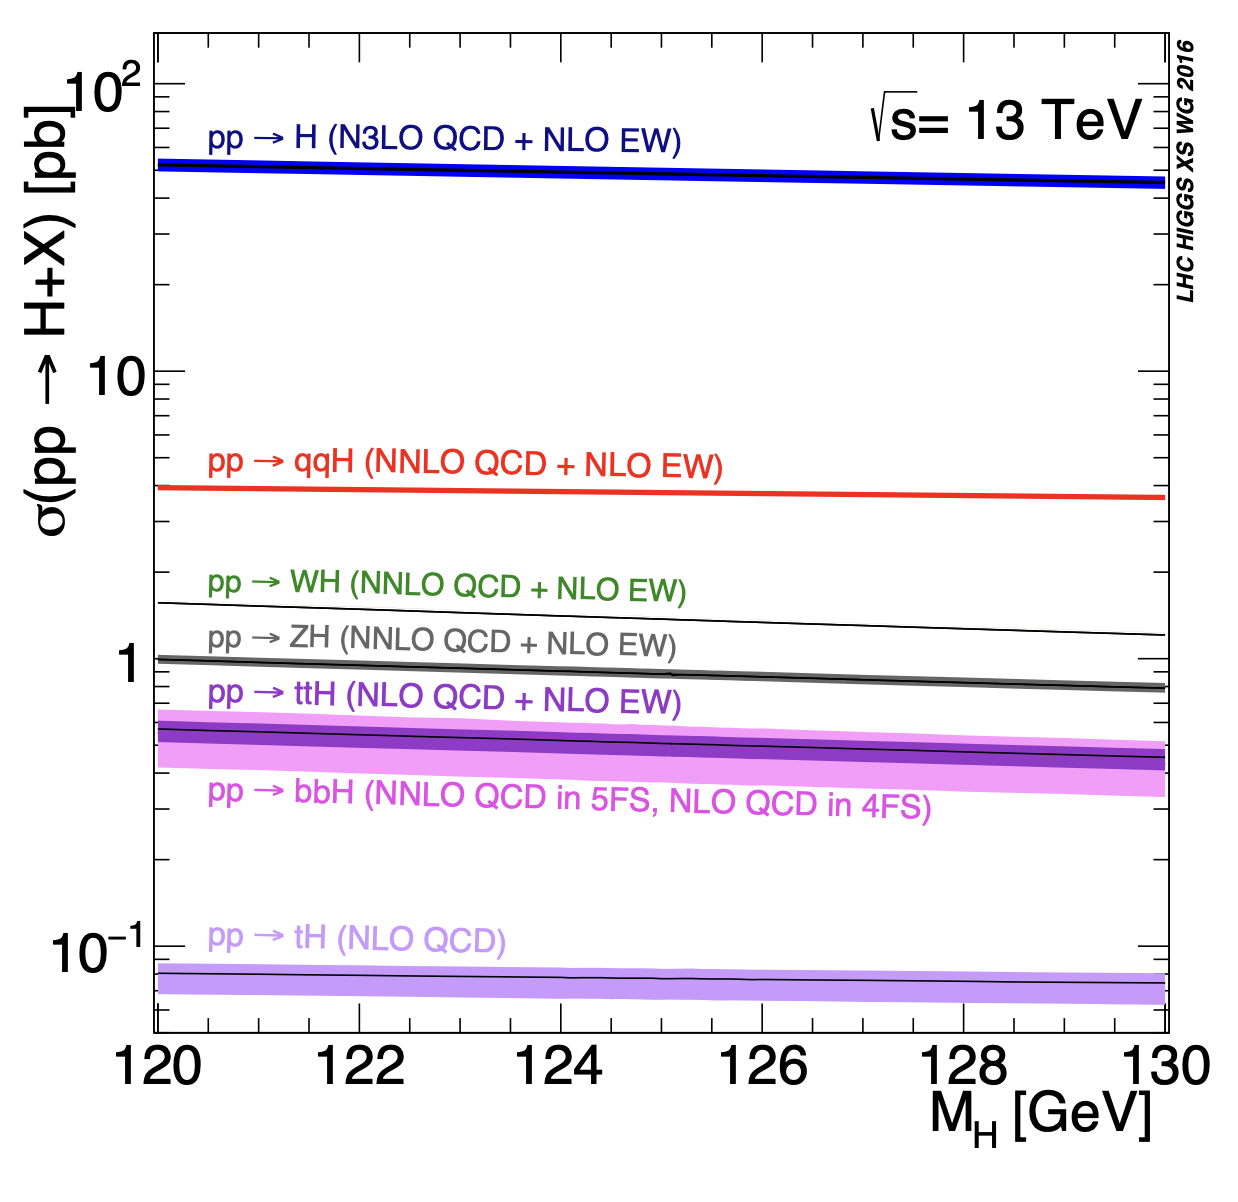
\includegraphics[width=\textwidth]{figures/higgs-xs.png}
        \caption{Production cross-section}
        \label{subfig:higgs-production-xs}
    \end{subfigure}
    \begin{subfigure}[b]{0.48\textwidth}
        \centering 
        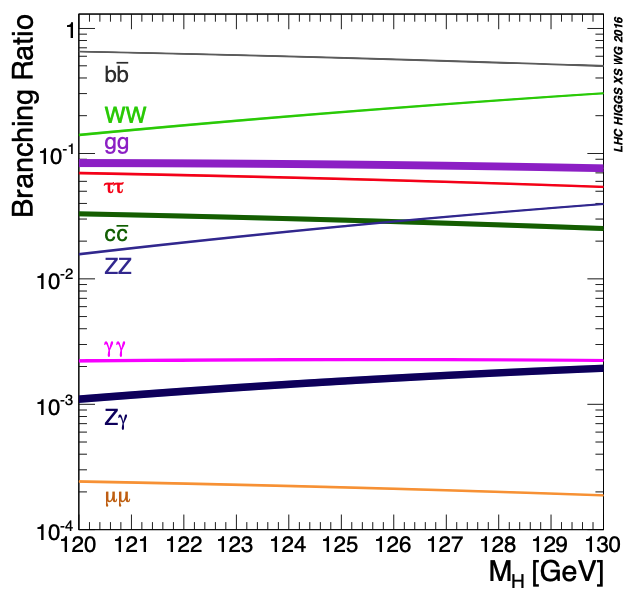
\includegraphics[width=\textwidth]{figures/higgs-branching-ratios.png}
        \caption{Branching ratio of Higgs decay}
        \label{subfig:higgs-br}
    \end{subfigure}
    \caption{Production cross-section of the Standard Model Higgs boson produced by $pp$ collision as a function of $M_H$ at $\sqrt{s}=13$ TeV}
    \label{fig:higgs-production-decay}
\end{figure}

The most dominant production mechanism is gluon-gluon fusion, whose cross-section far exceeds those of other mechanism. The Feynman diagram for this process is shown in figure \ref{subfig:gg-fusion-triangle}. The gluon is massless and only indirectly couples to the Higgs boson through a triangular heavy quark loop, to which the largest contribution comes from the top quark. The diagram still has a large magnitude, thanks to the strong coupling of the Higgs boson and the gluon to the top quark at this energy scale. 

Production via vector boson fusion $(VBF)$ sees the second largest cross-section, thanks to large couplings between the Higgs and the $W/Z$ bosons and between the vector bosons to heavy quarks, albeit an order of magnitude smaller than $\sigma_{ggF}$. Its tree-level diagram is shown in figure \ref{subfig:vbf}. The final state is characterized two forward jets from hadronized heavy quarks, along with products from various Higgs decay signatures. This process is particularly important in measurements of the $g_{HVV}$ coupling.

The leading diagram for associated Higgs production with a vector boson initiated by a pair of quarks $(qq\rightarrow VH)$ is shown in figure \ref{subfig:VH-higgs}. Another much smaller $gg$-initiated production also contribute at next-to-leading order. The Higgs boson is produced via Higgsstrahlungs from the vector boson. The letter can decay leptonically or hadronicall, but analyses in the leptonic channel often benefit from efficient lepton triggers, and high-quality lepton reconstruction. 

Finally, we mention the mechanism of associated production with a top quark pair, shown in figure \ref{subfig:ttH-signature}, which is small but of paramount importance in probing the Higgs coupling to the top quark. Unlike the case of other third-generation fermions, namely the tau lepton and the bottom quark, the Higgs decay to the top quark is kinematically forbidden due to the latter's large mass. Therefore, the top quark Yukawa coupling $y_t$ can only be measured through the $pp\rightarrow t\bar{t}H$ production process. 

\begin{figure}[h]
    \centering
    \begin{subfigure}[b]{0.48\textwidth}
        \centering
        \begin{tikzpicture}
          \begin{feynman}
            \vertex (t1) at (0,0);
            \vertex (t2) at (-0.866, 0.5);
            \vertex (t3) at (-0.866, -0.5);
            \vertex [above left = of t2] (a);
            \vertex [below left = of t3] (b);
            \vertex [right = of t1] (c);
            \diagram[horizontal = t1 to c] {
                (t1) -- [scalar, edge label=\(H\)] (c),
                (t1) -- [fermion, edge label=\({t}\)] (t3)  -- [fermion, edge label=\({t}\)] (t2) --[fermion, edge label=\({t}\)] (t1),
                (a) -- [gluon] (t2),
                (b) -- [gluon] (t3),
            };
          \end{feynman}
        \end{tikzpicture}
        \vfill
        \caption{Triangular gluon-gluon fusion production}
        \label{subfig:gg-fusion-triangle}
    \end{subfigure}
    \hfill
    \begin{subfigure}[b]{0.48\textwidth}
        \centering
        \begin{tikzpicture}
          \begin{feynman}
            \vertex (h) at (0.3,0);
            \vertex (tgp) at (-0.3, 1) ;
            \vertex (bgp) at (-0.3, -1) ;
            \vertex (gt) at (-1.8, 1.2) {$q$};
            \vertex (gb) at (-1.8, -1.2) {$q'$};
            \vertex (t) at (1.4, 1.2) {$q$} ;
            \vertex (b) at (1.4, -1.2) {$q'$};
            \vertex (htb) at (1.5, 0) {$H$};
            \diagram[] {
                (h) -- [photon, edge label = \($W/Z$\)] (tgp),
                (bgp) -- [photon, edge label = \($W/Z$\)] (h),
                (gt) -- [fermion] (tgp),
                (gb) -- [fermion] (bgp),
                (tgp) -- [fermion] (t),
                (bgp) -- [fermion] (b),
                (h) -- [scalar] (htb),
            };
          \end{feynman}
        \end{tikzpicture}
        \vfill
        \caption{Vector boson fusion production}
        \label{subfig:vbf}
    \end{subfigure}
    \vfill
    \begin{subfigure}[b]{0.48\textwidth}
        \centering
        \begin{tikzpicture}
          \begin{feynman}
            \vertex (t1) at (0,0);
            \vertex (t2) at (-0.7, 1.5) {$\bar{q}$};
            \vertex (t3) at (-0.7, -1.5) {$q$};
            \vertex (t4) at (2, 0.);
            \vertex (t5) at (2.7, 1.5) {$W/Z$};
            \vertex (t6) at (2.7, -1.5) {$H$} ;
            \diagram[] {
                (t1) -- [fermion] (t2),
                (t3) -- [fermion] (t1),
                (t1) -- [photon, edge label = \(W/Z\)] (t4),
                (t4) -- [photon] (t5),
                (t4) -- [scalar] (t6),
            };
          \end{feynman}
        \end{tikzpicture}
        \caption{Associated production with a vector boson}
        \label{subfig:VH-higgs}
    \end{subfigure}
    \begin{subfigure}[b]{0.48\textwidth}
        \centering
        \begin{tikzpicture}
          \begin{feynman}
            \vertex (h) at (0,0);
            \vertex (tgp) at (-0.3, 1) ;
            \vertex (bgp) at (-0.3, -1) ;
            \vertex (gt) at (-1.8, 1.2) {$g$};
            \vertex (gb) at (-1.8, -1.2) {$g$};
            \vertex (t) at (1.4, 1.2) {$q$} ;
            \vertex (b) at (1.4, -1.2) {$\bar{q}$};
            \vertex (htb) at (1.5, 0) {$H$} ;
            \diagram[] {
                (h) -- [fermion] (tgp),
                (bgp) -- [fermion] (h),
                (gt) -- [gluon] (tgp),
                (gb) -- [gluon] (bgp),
                (tgp) -- [fermion] (t),
                (b) -- [fermion] (bgp),
                (h) -- [scalar] (htb),
            };
          \end{feynman}
        \end{tikzpicture}
        \caption{Associated production with top quark pair}
        \label{subfig:ttH-signature}
    \end{subfigure}
    \caption{Leading-order Higgs boson production mechanisms}
    \label{fig:higgs-production}
\end{figure} 

Another consequence of the Higgs coupling structure described in \ref{sect:Higgs-mechanism} equally important to the study of the Higgs boson at the LHC is the consideration of its decay channels. 
Being one of the heaviest SM particles, the Higgs boson has a lifetime of approximately $10^{-22}s$. 
Tree-level Higgs boson decay is induced by its coupling to quarks, whose primary channels include $H\rightarrow b\bar{b}/c\bar{c}$, to leptons, namely $H\rightarrow \tau\bar{\tau}/\mu\bar{\mu}$, and to vector bosons, namely $H\rightarrow WW/ZZ$. 
In addition, notable loop-induced decays include $H\rightarrow gg/\gamma\gamma/Z\gamma$. Figure \ref{subfig:higgs-br} shows the branching ratios of primary Higgs decay channels as a function of the Higgs mass near $m_H=125$ GeV. Table \ref{tab:higgs-br} specifies the branching ratio measured at Higgs mass $M_H=125.09$ GeV.

\begin{table}[h]
    \centering
    \begin{tabular}{|l|c|}
    \hline \hline
     Decay channel    & Branching ratio $(\%)$ \\
     \hline
      $H\rightarrow b\bar{b}$   & $57.5\pm 1.9$ \\
      $H\rightarrow WW $   & $21.6\pm0.9$ \\
       $H\rightarrow gg$  & $8.56\pm0.86$ \\
        $H\rightarrow \tau\bar{\tau}$    & $6.30\pm 0.36$ \\
        $H\rightarrow c\bar{c}$    & $2.9\pm 0.35$ \\
        $H\rightarrow ZZ$    & $2.67\pm 0.11$ \\
        $H\rightarrow \gamma\gamma$    & $0.228\pm 0.011$ \\
        $H\rightarrow Z\gamma$    & $0.155\pm 0.014$ \\
        $H\rightarrow \mu\bar{\mu}$    & $0.022\pm 0.001$ \\
    \hline
    \end{tabular}
    \caption{Standard Model Higgs boson decay branching ratios and uncertainty at $M_H=125.09$ GeV}
    \label{tab:higgs-br}
\end{table}

Since a decay to the top quark is forbidden, it is not surprising that the most dominant decay mode is the $H\rightarrow b\bar{b}$ via Yukawa coupling, whose branching ratio is $57.5\%$ at $m_H=125.09$ GeV. 
Among other fermions, decay into a pair of tau leptons is the second largest, followed by decays into second-generation fermions (figure \ref{subfig:hff-decay}). 
The decay to a pair of vector boson proceeds through tree-level processes (figure \ref{subfig:hVV-decay}), whereas $H\rightarrow \gamma\gamma$ is mediated by a $W$ boson (figure \ref{subfig:hyy-W}) or a heavy quark loop (figure \ref{subfig:H-yy-t}). Despite having a small branching ratio, $H\rightarrow \gamma\gamma$ is an important channel for precision measurement of the Higgs mass due to the high resolution of the reconstructed photon invariant mass. 

\begin{figure}[h!]
    \centering
    \begin{subfigure}[b]{0.48\textwidth}
        \centering
        \begin{tikzpicture}
          \begin{feynman}
            \vertex (h) at (0,0) {$H$};
            \vertex [right = of h] (hff) ;
            \vertex [above right = of hff] (f1) {$b,\tau,c$};
            \vertex [below right = of hff] (f2) {$\bar{b}, \bar{\tau}, \bar{c}$};
            \diagram[horizontal = h to hff] {
                (h) -- [scalar] (hff),
                (hff) -- [fermion] (f1),
                (f2) -- [fermion] (hff),
            };
          \end{feynman}
        \end{tikzpicture}
        \vfill
        \caption{Higgs decay to fermions}
        \label{subfig:hff-decay}
    \end{subfigure}
    \hfill
    \begin{subfigure}[b]{0.48\textwidth}
        \centering
        \begin{tikzpicture}
          \begin{feynman}
            \vertex (h) at (0,0) {$H$};
            \vertex [right = of h] (hvv) ;
            \vertex [above right = of hvv] (v1) {$W/Z$};
            \vertex [below right = of hvv] (v2) {$W/Z$};
            \diagram[horizontal = h to hvv] {
                (h) -- [scalar] (hvv),
                (hvv) -- [photon] (v1),
                (hvv) -- [photon] (v2),
            };
          \end{feynman}
        \end{tikzpicture}
        \vfill
        \caption{Higgs decay to vector bosons}
        \label{subfig:hVV-decay}
    \end{subfigure}
    \vfill
    \begin{subfigure}[b]{0.48\textwidth}
        \centering
        \begin{tikzpicture}
          \begin{feynman}
            \vertex (h) at (0,0) {$H$};
            \vertex [right = of h] (hff) ;
            \vertex [above right = of hff] (f1) ;
            \vertex [below right = of hff] (f2) ;
            \vertex [right = of f1] (y1) {$\gamma$};
            \vertex [right = of f2] (y2) {$\gamma$};
            \diagram[horizontal = h to hff] {
                (h) -- [scalar] (hff),
                (hff) -- [fermion, edge label = \($t$\)] (f1) -- [fermion, edge label = \($t$\)]
                (f2) -- [fermion, edge label = \($t$\)] (hff),
                (f2) -- [photon] (y2),
                (f1) -- [photon] (y1),
            };
          \end{feynman}
        \end{tikzpicture}
        \caption{$H\rightarrow \gamma\gamma$ decays via $t$-loop}
        \label{subfig:H-yy-t}
    \end{subfigure}
    \begin{subfigure}[b]{0.48\textwidth}
        \centering
        \begin{tikzpicture}
          \begin{feynman}
            \vertex (h) at (0,0) {$H$};
            \vertex [right = of h] (hff) ;
            \vertex [above right = of hff] (f1) ;
            \vertex [below right = of hff] (f2) ;
            \vertex [right = of f1] (y1) {$\gamma$};
            \vertex [right = of f2] (y2) {$\gamma$};
            \diagram[horizontal = h to hff] {
                (h) -- [scalar] (hff),
                (hff) -- [photon, edge label = \($W$\)] (f1) -- [photon, edge label = \($W$\)]
                (f2) -- [photon, edge label = \($W$\)] (hff),
                (f2) -- [photon] (y2),
                (f1) -- [photon] (y1),
            };
          \end{feynman}
        \end{tikzpicture}
        \caption{$H\rightarrow \gamma\gamma$ decays via $W$-loop}
        \label{subfig:hyy-W}
    \end{subfigure}
    \caption{Leading-order Higgs boson decay mechanisms}
    \label{fig:higgs-decays}
\end{figure} 

\section{Extension of the Standard Model Higgs sector}
\label{sect:introduce-2HDM}

Until now, we have given a theoretical description of the simplest possible scalar structure of the Higgs field, namely a single $SU(2)$ doublet $\phi$. 
This assumption is motivated almost entirely by simplicity, and there exist a number of extensions to the SM Higgs sector which satisfy the experimental constraint on its scalar structure \cite{Zyla:2020zbs}. 
The simplest of such extensions consists of an additional scalar Higgs doublets--known as the two-Higgs-doublet model (2HDM). 

The model is motivated by several considerations, the best know of which is supersymmetry, which is explored in Ref. \cite{HABER198575}. Briefly speaking, supersymmetric quarks of charges $2/3$ and $-1/3$ cannot acquire their mass through coupling to a single Higgs doublet. Moreover, the cancellation of anomalies requires the existence of an additional Higgs doublet. Therefore, the Minimal Supersymmetric Standard Model (MSSM) must contain two Higgs doublets, as prescribed by the 2HDM.

In addition, while the SM cannot account for the baryon-antibaryon asymmetry of the early universe, the 2HDM, thanks to the flexibility of their scalar mass spectrum and additional sources of CP violation, can provide stronger theoretical explanation of this phenomenon. Aspects of electroweak baryogenesis in the 2HDM is explored in reference \cite{Joyce_1996, Funakubo_1994, Cline_1996, PhysRevD.55.3873, LAINE200123, LarsFromme_2006}. A comprehensive review of the rich phenomenology of the 2HDM can be found in Ref. \cite{Branco_2012}.

In the context of dark matter (DM) searches at the LHC, the 2HDM extended by a pseudo-scalar mediator $a$, denoted by \thdma, constitute an attractive benchmark model \cite{2HDMWGproxi}. The pseudo-scalar mediates the interactions between the visible sector of the 2HDM and the dark sector, assumed to include a single fermionic DM particle $\chi$. Chapter \ref{chap:combination-dark-matter-2hdma} presents a combination and summary of dark matter searches using $139\, \ifb$ of $pp$ collision data at $\sqrt{s}=13$ TeV collected by the ATLAS detector throughout LHC Run 2. 
Relevant phenomenological aspects of the \thdma are presented in \ref{sect:theoretical-considerations-2hdma}, along with important model parameters and experimental signatures to be examined by DM searches in ATLAS, many of which are introduced earlier in this chapter. 
\chapter{The ATLAS experiment}
\label{chap:ATLAS-detector}

% \section{The Large Hadron Collider (LHC) and its detectors}

% The Large Hadron Collider belongs to a class of particle accelerators called synchrotrons, of which CERN constructs and operates many examples. The synchrotron allows accelerating particles in a close-loop 

% % Introduce in this section
% % \begin{itemize}
% %     \item Generalities of the LHC
% %     \item Luminosity and pile-up
% % \end{itemize}

\section{The ATLAS detector}
The ATLAS (A Toroidal LHC ApparatuS) detector is one of the two general-purpose detectors, along with CMS, designed to observe any new physics phenomena that the LHC can discover. It is a cylindrical structure constructed around the beam pipe at one of the collision points on the LHC, comprised of an Inner Detector (ID), an electromagnetic calorimeter, a hadronic calorimeter, and a muon spectrometer. Being the largest of the LHC detectors, it spans 44m in length and 25m in height, as shown in figure \ref{fig:atlas-schematic}.

The detector's geometry facilitates the use of a right-handed cylindrical coordinate system to describe locations and directions, with the nominal interaction point (IP) at the origin. The $z$-axis points along the beam pipe, parallel to the direction of the incoming protons. The $x$-axis points from the IP towards the center of the LHC. Any position is described by $(r, \phi, z)$, where $\phi \in [-\pi, \pi)$. Particle momentum can be represented by a four-vector $p=(E, p_x, p_y, p_z)$. In practice, however, the rapidity, define as 
\begin{equation}
    \label{eq:3.1}
    y = \frac{1}{2}\ln\left( \frac{E+p_z}{E-p_z} \right)
\end{equation}
is commonly used in lieu of the longitudinal momentum, because differences in rapidity is invariant under a Lorentz boost along $z$. For massless or very energetic particles, the rapidity is well approximated by the pseudorapidity defined from the polar angle $\theta$
\begin{equation}
    \label{eq:3.2}
    \eta = -\ln \tan \left ( \frac{\theta}{2} \right).
\end{equation}
Both $y$ and $\eta$ are symmetric about $z=0$. A particle moving entirely on the transverse plane has $y=\eta=0$, and one moving parallel to the $z$-axis has $\eta=\pm\infty$. Obviously, no detector can cover the entire $4\pi$ steradians of solid angle around the IP. The range of pseudorapidity observable by a detector is called the \textit{acceptance}. Each subsystem of ATLAS has a different acceptance, in particular, $\abs{\eta}<2.5$ in the ID, and $\abs{\eta}<4.8$ for the calorimeters. Since the pseudorapidity represents the polar angle, it is sufficient to describe a particle by $(E, p_T, \eta, \phi)$, where $p_T = \sqrt{p_x^2 + p_y^2}$ is the transverse momentum.

\begin{figure}[h!]
    \centering
    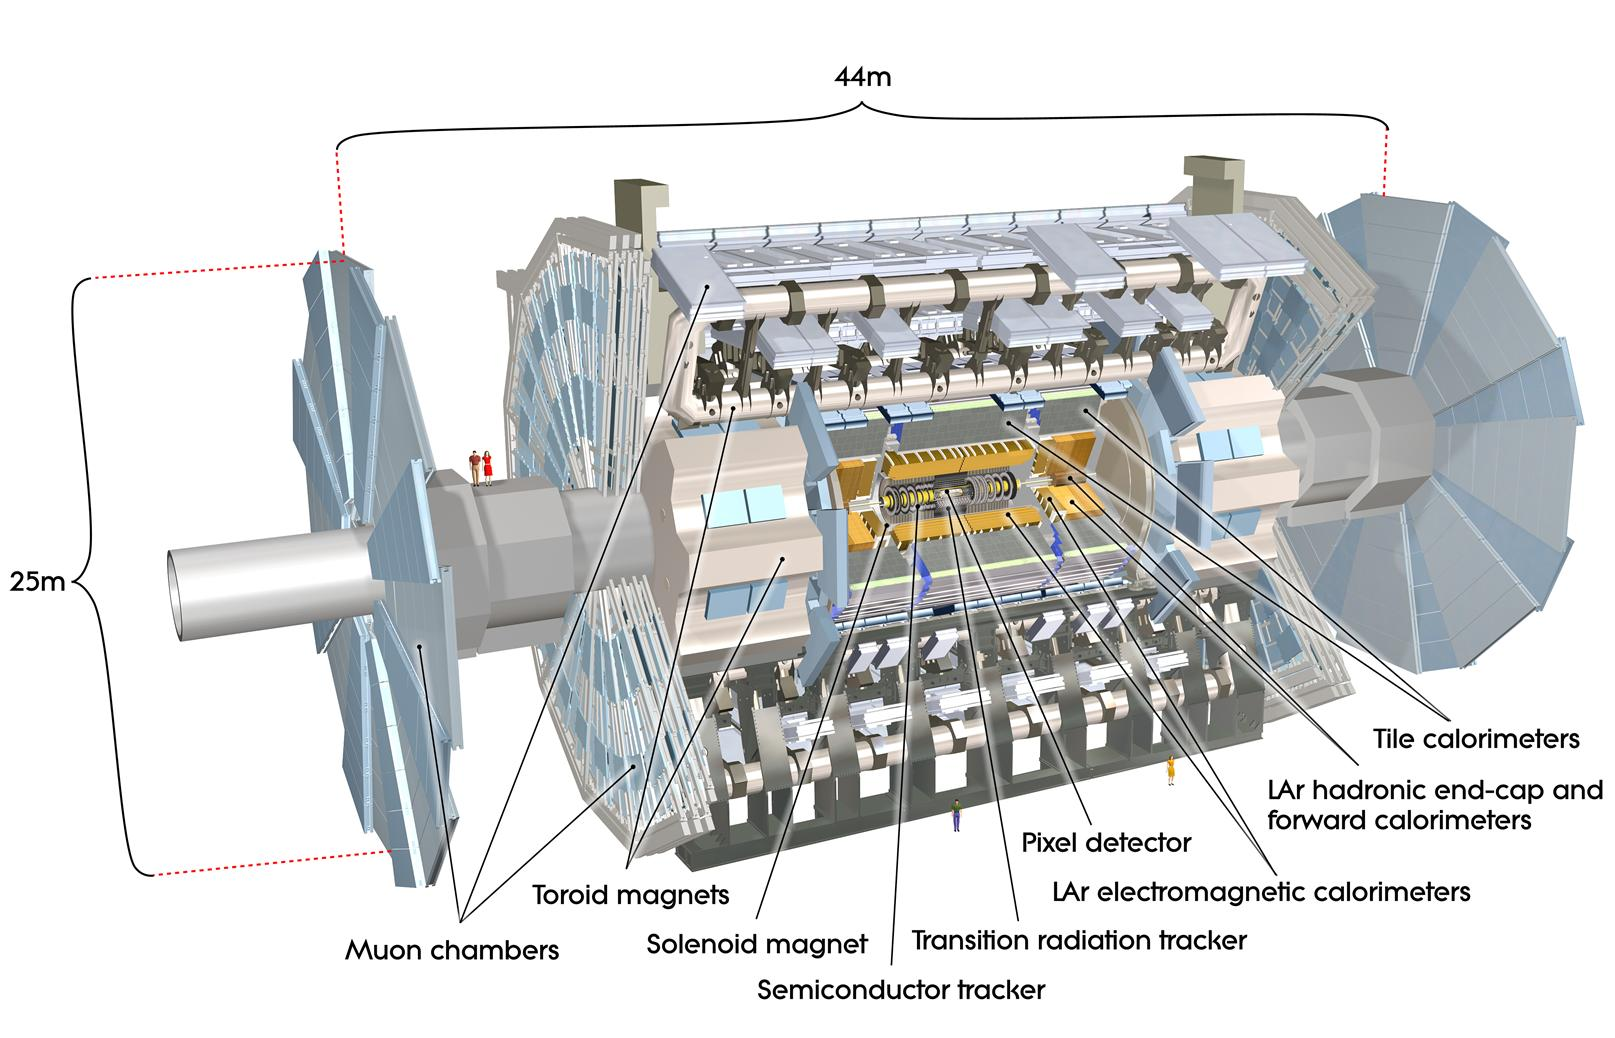
\includegraphics[width=0.9\linewidth]{figures/atlas.jpg}
    \caption{The ATLAS detectors and its components \cite{Pequenao:1095924}}
    \label{fig:atlas-schematic}
\end{figure}

\subsection{The Inner Detector}
\label{subsect:inner-detector}f
Immediately surrounding the interaction point is the Inner Detector, consisting of 3 subsystems constructed from two sensing technologies. These subsystems include a Pixel detector, a Semi-Conductor Tracker (SCT), and a Transition Radiation Tracker (TRT), in the same order of increasing radial distance from the IP. The first two use silicon sensors to detect the passage of a charged particle and the latter a collection of gas-filled straw tube and a tungsten wire to collect the secondary radiation engendered from the particle.

The ID is responsible for precise measurements of discrete points along the path of a charged particle, from which its trajectory (tracks) is reconstructed. Tracks are essential inputs to reconstruct physics objects charged leptons, jets, as well as the identification of jets from heavy quarks. 

A crucial part of the ID's function is the estimation of particle momentum and impact parameters. In the presence of a homogeneous magnetic field of 2T permeating the ID along the $z$-axis, charged particles move in helical orbits, whose radius depends on the transverse momentum $p_T$
\begin{equation}
    \label{eq:3.3}
    R = \frac{p_T}{qB}.
\end{equation}
In principle, by fitting a helix through measurements on a track, one obtains an estimate of the curvature and thus $p_T$. Extrapolating this helix to the point of closest approach to the IP, called the \textit{perigee}, one obtains an estimate of the primary and longitudinal impact parameters $(d_0, z_0)$ respectively. This procedure is described in detail in chapter \ref{chap:atlas-reco-chain}. 

Being the first sub-detector to observe particles after they are created in the entire detector, the ID has the best position to characterize their kinematics to the highest possible resolution. In particular, the relative momentum resolution $p_T\sigma(\frac{q}{p_T})$ is $O(1\%)$, while the impact parameter resolutions can reach $\sigma(d0)\approx 25\mu m$ and $\sigma(z0)\approx 40\mu m$. This level of resolution is remarkable considering the physical dimensions of ATLAS, which can only be achieved through meticulous custom designs of the subsystems described below.

\subsubsection{The Pixel Detector}
The pixel detector (figure \ref{fig:atlas-pixel}) is the innermost part of the ID, consisting of 3 barrel layers extending from a radius of $r=50.5\, mm$ up to $r=122.5\, mm$, and 3 end-cap disks on each sides of the barrel. These physical layers each provide a structure onto which detector modules are mounted. Each barrel layer consists of supporting staves  from pixel modules mounted on supporting staves, and each end-cap from 8 sectors circularly arranged around the $z$-axis, each containing 6 modules. In total, the pixel detector has 1744 identical modules, each composed of an array of silicon sensor and 16 front-end chips which read out the electrical signal created by the passage of a charge particle. \cite{front-end-chips} 

A sensor element is fabricated from a detector-grade n-type silicon wafer implanted with high positive ($p^+$) and negative ($n^+$) dose regions on each side. At the $p^+$-$n$ junction, holes from the $p^+$ region neutralize free electrons in the $n$-typed bulk, creating a depletion zone devoid of free charge carriers. Operated in a reverse bias, this region is enlarged over the whole sensor bulk volume. Although containing no free charge carrier, the $pn$-junction is easily ionized by a traversing particle, creating electron-hole pairs. Primary electrons, those directly created by the traversing particle, are often energetic enough to induce secondary ionization and amplify the signal. Electron-hole pairs are separated by the biasing electric field and drift toward their corresponding electrodes. As electrons approach the anode, they are multiplied and measured by the read-out chips.

The sensitive part of a pixel module is approximately $2\times 6\,cm^2$ in size, segmented into highly granular pixels of dimensions $50\times 400 \, \mu m^2$, totalling 47268 pixels. Nearly every pixel corresponds to a readout channel, providing the pixel detector approximately 80 million channels. With the inclusion of the Insertable B-Layer (IBL), the total number of channels the smallest pixel dimension is reduced to $50\times 250$ $\mu m^2$, and the total number of readout channels increased to $94$ million. This high level of granularity enables high precision measurements very close to the beam pipe. The eta

\begin{figure}[h!]
     \centering
     \begin{subfigure}[b]{0.49\textwidth}
         \centering
         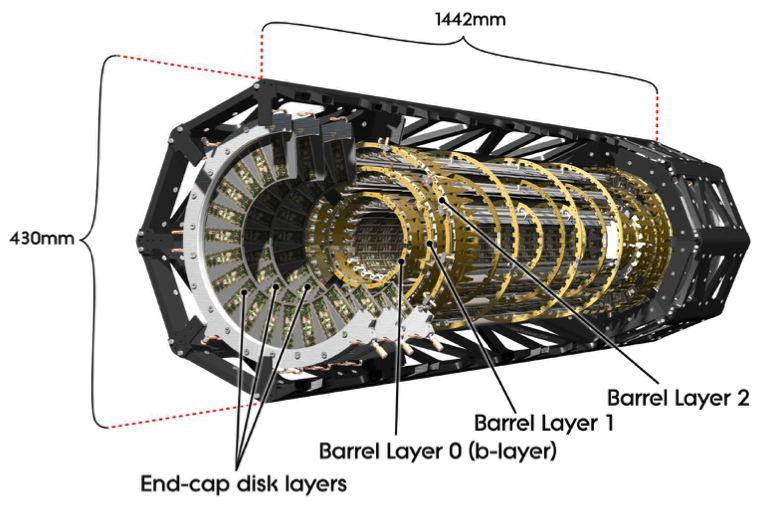
\includegraphics[width=\textwidth]{figures/pixel-detector.png}
         \caption{The ATLAS pixel detector}
         \label{fig:atlas-pixel}
     \end{subfigure}
     \hfill
     \begin{subfigure}[b]{0.49\textwidth}
         \centering
         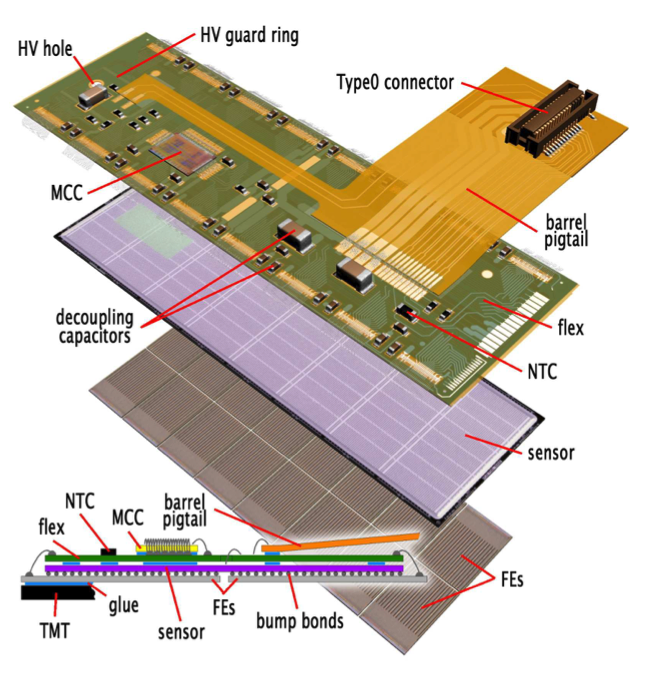
\includegraphics[width=\textwidth]{figures/pixel-module.png}
         \caption{The pixel detector module}
         \label{fig:pixel-module}
     \end{subfigure}
    \caption{The ATLAS pixel detector and detector module. Figures taken from reference~\cite{ID-pixel}}
    \label{fig:pixel-detector-and-module}
\end{figure}

\subsubsection{The Semi-Conductor Tracker}

Surrounding the Pixel volume is the Semi-Conductor Tracker (SCT), consisting of four barrel layers and eighteen symmetric end-cap disks, both featuring a total of 4088 strip modules \cite{ATLAS-TDR-04, ATLAS-TDR-05}. Figure \ref{subfig:strip-module} provides an overview of a strip module used in the barrel layers. Each detector module consists of two pairs of single-sided microstrips with $80$ $\mu m$ pitch. Each single strip sensor is capable of detecting particle intersection in one dimension, information from a pair of strips must be combined to provide three-dimensional point information with space-point resolution of 16 $\mu m$ in the $(R-\phi)$ direction and 580 $\mu m$ in the $z$-direction \cite{BARONE201357}. 

\begin{figure}[h!]
     \centering
     \begin{subfigure}{0.7\textwidth}
         \centering
         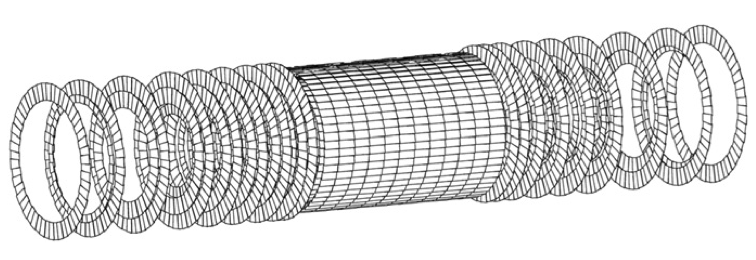
\includegraphics[width=\textwidth]{figures/sct-detector.png}
         \caption{The ATLAS pixel detector}
         \label{subfig:sct-detector}
     \end{subfigure}
     % \hfill
     \begin{subfigure}{0.65\textwidth}
         \centering
         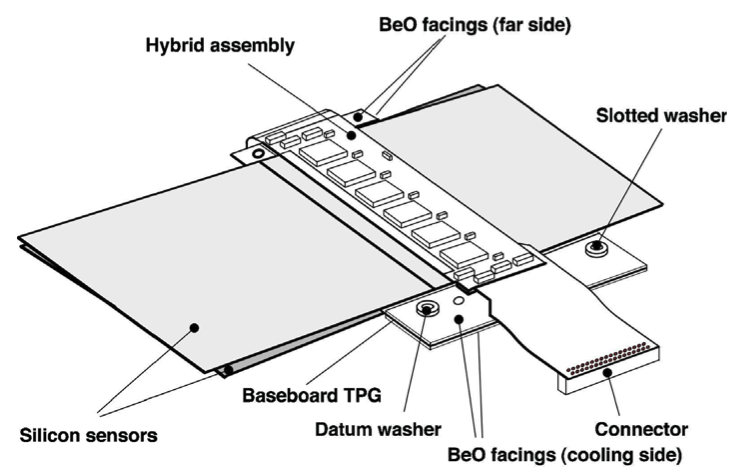
\includegraphics[width=0.9\textwidth]{figures/strip-module.png}
         \caption{The pixel detector module}
         \label{subfig:strip-module}
     \end{subfigure}
    \caption{Overview of the strip module of the SCT in the barrel layers. Figures taken from reference~\cite{Robinson_2013}}
    \label{fig:sct-detector}
\end{figure}

% \begin{figure}[h!]
%     \centering
%     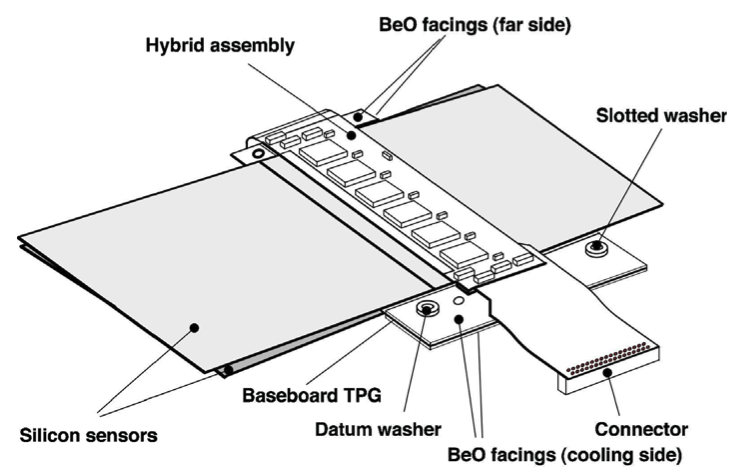
\includegraphics[width=0.5\linewidth]{figures/strip-module.png}
%     \caption{Overview of the strip module of the SCT in the barrel layers}
%     \label{fig:strip-module}
% \end{figure}

\subsubsection{The Transition Radiation Tracker}
The Transition Radiation Tracker (TRT) is the outermost component of the Inner Detector. It comprises of approximately 300000 straw tubes that are 4 $mm$ in diameter, and covers up to $\abs{\eta}=1$ in the barrel and $\abs{\eta} =2$ in the end-cap layers. Each high $p_T$ track passing through the TRT leaves $30-36$ hits and reach a resolution of 130 $\mu m$ in the $(R-\phi)$ direction. 

In each straw tube, a tungsten wire is located at the center and surrounded by a gas mixture spreading the volume of the tube. When a charged particle passes through the tube, it ionizes the ambient gas and creates an pairs of electrons and positive gas ions. An electric field exists between the outer tube and the central wire, which now act as electrodes, separating the charges. As they reach the wire, the charges are amplified and detected. To enhance electron identification, the straw tubes are surrounded by polymer fibers (barrel) and foils (end-caps), which facilitate transition radiation at the interface between materials. 

\subsection{The Calorimeter system}

The second group of detector subsystems, the calorimeters, is dedicated to the measurement of particle energies and directions. There exist two types of calorimeters: electromagnetic and hadronic. 
They detect particle through alternating layers of passive and active materials. 
In the passive layers, also called the absorber, an energetic particle deposits a large portion of its kinetic energy and induces a large number of secondary particles, including electrons, photons, and hadrons, depending on the type of calorimeter. 
These particles are then stopped and measured by the active layers. 

The electromagnetic calorimeter targets electrons/positrons and photons, which create electromagnetic showers as they interact with the inactive material. In the electric field near the atomic nuclei that make up the material, electrons and position undergo Brehmsstrahlung and emit secondary photons, which induces electron pair production in the vicinity of atomic nuclei and generates more high-energy charged particles. 
A reaction chain in which Brehmsstrahlung photons induce electrons/positrons, which emits more Brehmsstrahlung photons, creates a shower of charged particles in the passive material. 

In the case of the hadronic calorimeters, hadrons passing through a dense material interact with its nuclei and produce secondary hadrons, mostly pions, which then drives the reaction chain, similar to the electromagnetic counterpart. In addition, neutral pion decays to high-energy photon and leptonic decays can also induce electromagnetic subshower within a hadronic shower. 

\subsubsection{The electromagnetic (EM) calorimeter}
The passive absorber material in the ATLAS electromagnetic calorimeter comprises of lead, and the active material of liquid argon. The passive layers are interspersed with active layers in an accordion pattern. The barrel covers a pseudoscalar range up to $\abs{\eta} = 1.475$ and the endcaps $1.375 < \abs{\eta}<3.2$. The central region of the EM calorimeter consists of three layers and a pre-sampler with a fine granularity $(\eta\times\phi=0.025\times 0.1)$. The first sampling layer features a segmentation of $\eta\times\phi=0.025/8\times 0.1$, while the second and third sampling layers are segmented into $\eta\times\phi=0.025\times 0.025$ and $\eta\times\phi=0.025\times 0.05$, respectively. Angular segmentation allows measurements of particle directions, and depth segmentation measurements of shape. This information is in turn useful in discriminating electrons and photons from jets. Figure \ref{subfig:em-calorimeter-module} shows a sketch of the EM calorimeter module in the barrel. 

\begin{figure}[h!]
    \begin{subfigure}[b]{0.59\textwidth}
    \centering
    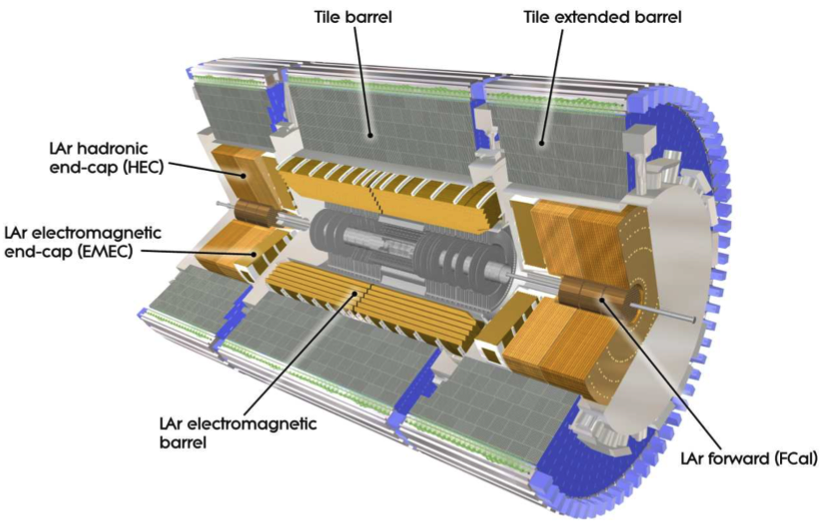
\includegraphics[width=\textwidth]{figures/calorimeter-system.png}
    \caption{}
    \label{subfig:calorimeter-system}
    \end{subfigure}
    \hfill
    \begin{subfigure}[b]{0.4\textwidth}
    \centering
    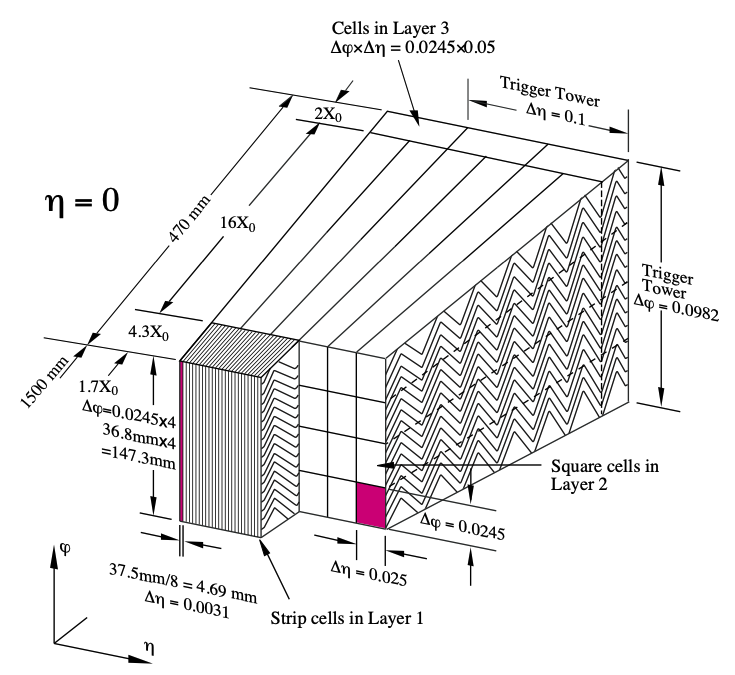
\includegraphics[width=\textwidth]{figures/Em-calorimeter.png}
    \caption{}
    \label{subfig:em-calorimeter-module}
    \end{subfigure}
    \caption{(a) Layout of the ATLAS calorimetry system, and (b) sketch of a barrel module of the electromagnetic calorimeter~\cite{atlas_exp_2008}.}
    \label{fig:calorimeter}
\end{figure}

\subsubsection{The hadronic calorimeter}
The hadronic calorimeter uses iron absorbers and plastic scintillating tiles as active material in the barrel region. It covers a pseudorapidity range of $\abs{\eta} < 1.0$ in the barrel and $0.7 < \abs{\eta} < 1.7$ in the extended barrel. It also comprises of three layers of increasing radii. The effective granularity varies between $\eta\times\phi=0.1\times 0.1$ and $0.2\times 0.1$. 

The endcap and forward regions (figure \ref{subfig:calorimeter-system}) of the hadronic calorimeter uses copper/tungsten as absorber and liquid Argon as active material. They cover a pseudorapidity range of up to 4.9. The forward calorimeter is split into an electromagnetic and a hadronic component. 

\subsection{The muon spectrometer}
Unlike other particles, muons produced with energy in the range of $0.1-100$ GeV typically seen in ATLAS do not strongly interact with detector material in the detector subsystems described in the previous sections. Despite leaving energy clusters in the ID, they traverse the calorimeters intact are therefore measured by a dedicated muon system. The muon spectrometer is composed of four subsystems that use different technologies to 
track muon at high precision and perform fast triggers. It is immersed in a toroidal magnetic field ranging from 2.0 to 6.0 T, providing enough bending power to resolve the muon transverse momentum. Figure \ref{fig:MS-system} shows the overall layout of and a side view of a quadrant of the MS, including its subsystems. 

\begin{figure}[h!]
    \begin{subfigure}[b]{0.4\textwidth}
    \centering
    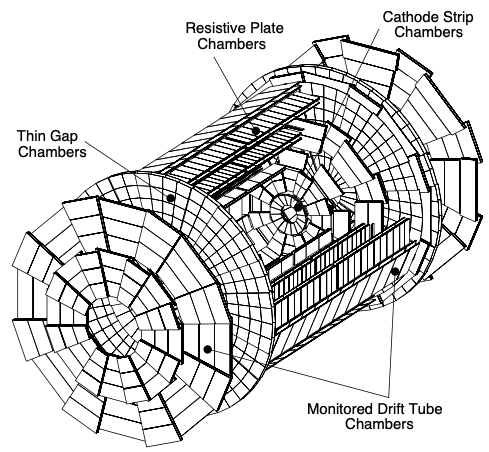
\includegraphics[width=\textwidth]{figures/MS-overview.png}
    \caption{}
    \label{subfig:MS-system-overview}
    \end{subfigure}
    \hfill
    \begin{subfigure}[b]{0.59\textwidth}
    \centering
    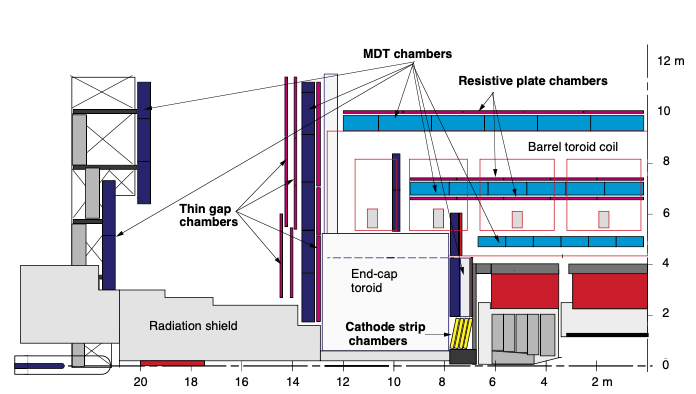
\includegraphics[width=\textwidth]{figures/MS-sideview.png}
    \caption{}
    \label{subfig:MS-system-sideview}
    \end{subfigure}
    \caption{(a) Layout of the ATLAS Muon Spectrometer system, and (b) a sideview of one quadrant of the MS~\cite{ATLAS-TDR-10}.}
    \label{fig:MS-system}
\end{figure}

To measure the curvature of muon tracks along the bending direction of the toroidal field, the MS uses a number of aluminum tubes of 30 milimeters in diameter filled with Ar and having a central tungsten/rhenium alloy wire, similar to the TRT. The outer surface and the central wire of these Monitored Drift Tubes (MDTs) are kept at a potential difference of 3 kV to ensure a drifting time of less than 700 ns. The MDTs are divided into 1200 chambers cover a pseudorapidity range up to $\abs{\eta} =2.7$, each chamber providing 6 to 8 measurements along the track.

At larger $\abs{\eta}$, the Cathode Strip Chambers (CSCs) have a higher granularity than the MDTs to resolve large backgrounds in the forward region. They cover $2.0< \abs{\eta} < 2.7$ and have short drift times of around $40$ ns. The CSCs provide 4 simultaneous measurements of $\eta$ and $\phi$.

The Resistive Plate Chambers (RPCs), used in the barrel and the Thin Gap Chambers (TGCs), used in the endcap regions are both gaseous detectors and together make up the muon trigger system. They respectively cover $\abs{\eta} < 1.05$ and $1.05 < \abs{\eta} < 2.4$.

% \subsection{The magnet system}

% \subsection{Trigger and Data Acquisition System}

% \section{Summary}

\chapter{Combination of dark matter searches interpreted in \thdma}
\label{chap:combination-dark-matter-2hdma}

This chapter presents the combined searches for dark matter particles in the context of a Two-Higgs-Doublet Model (2HDM) extended by a pseudoscalar mediator $a$ using proton-proton collision data collected at the ATLAS detector during LHC Run 2. 
We start with a discussion of the signal model as an extension of the Standard Model Higgs sector detailed in section \ref{sect:Higgs-mechanism}, and introduce the ferminonic dark matter particle $\chi$ connected to the visible sector via $a$.
In all analyses, no significant deviations from SM predictions are observed, and the data is used to derive exclusion limits on the signal model as functions of its parameters
A statistical combination of the most sensitive channels carries out the limit setting over six benchmark scenarios given in section \ref{sect:benchmark-scenarios}.
An overview of the experimental signatures targeted by theses searches, a description of systematic uncertainty, and the statistical method are provided in sections \ref{sect:exp-signatures}, \ref{sect:systematic-uncertainties} and \ref{sect:stat}, respectively.
Finally, the results are presented in section \ref{sect:combined-result}.
This analysis, in which the author is a contributor, has been published in reference \cite{2hdma_comb}.
 
\section{Theoretical considerations}
\label{sect:theoretical-considerations-2hdma}
The benchmark model used to interpret the data extends the Standard Model with a second complex Higgs doublet, already postulated in several UV-complete BSM theories \cite{Buckley:2014fba,Abercrombie:2015wmb}. After electroweak symmetry breaking, the model contains 5 Higgs bosons: a light CP-even boson $h$, a heavier CP-even boson $H$, a CP-odd boson $A$ and a two charged bosons $H^{\pm}$. The 2HDM allows some freedom in the choice of Higgs-fermion coupling structure, for example, 2HDM type-I which couples only one Higgs doublet to fermions, and 2HDM type-II, which couples the neutral member of one Higgs doublet to only up-type quarks and the neutral member of the other to down-type quarks. This search assumes the type-II structure, along with the alignment and decoupling limits, so that the lighter CP-even states $h$ can be identified with the SM Higgs boson \cite{Gunion:2002zf}. The Lagrangian of the 2HDM can be written as 
\begin{equation}
    \label{4.1}
    \mathcal{L}_{2HDM} = (D_{\mu}\Phi_1)^{\dag}(D^{\mu}\Phi_1) + (D_{\mu}\Phi_2)^{\dag}(D^{\mu}\Phi_2) - V(\Phi_1, \Phi_2)
\end{equation}
where the covariant derivative $D_{\mu}$ is given by 
$$D_{\mu} = \partial_{\mu} - ig\frac{\tau^i}{2}W^i_{\mu} - i\frac{g'}{2}YB_{\mu},$$
in which $\tau^i$ are Pauli matrices and $Y$ is the hypercharge. The potential is
\begin{equation} \label{4.2}
    \begin{split} 
        V(\Phi_1, \Phi_2)  &= m_{11}^2\Phi_1^{\dag}\Phi_1 + m_{22}^2\Phi_2^{\dag}\Phi_2 - (m_{12}^2 \Phi_1^{\dag}\Phi_2 + h.c.) \\
        &+ \frac{\lambda_1}{2}(\Phi_1^{\dag}\Phi_1)^2 + \frac{\lambda_2}{2}(\Phi_2^{\dag}\Phi_2)^2  
        + \lambda_3(\Phi_1^{\dag}\Phi_1)(\Phi_2^{\dag}\Phi_2) + \lambda_4 (\Phi_1^{\dag}\Phi_2)(\Phi_2^{\dag}\Phi_1) \\ 
        &+ \left\{ \frac{\lambda_5}{2} (\Phi_1^{\dag}\Phi_2)^2 + [\lambda_6(\Phi_1^{\dag}\Phi_1) + \lambda_7(\Phi_2^{\dag}\Phi_2) ](\Phi_1^{\dag}\Phi_2) + h.c. \right\} 
    \end{split}
\end{equation}
The scalar field vacuum expectation values occur at 
\begin{equation}
    \label{4.3}
    \expval{\Phi_i} = \frac{1}{\sqrt{2}}\begin{pmatrix}
        0 \\ v_i
    \end{pmatrix},\quad v_i \in \mathbb{R},
\end{equation}
with the following conditions
\begin{equation}
    \label{4.4}
    \begin{split}
        m_{11}^2 &= m_{12}^2 t_{\beta} - \frac{1}{2}v^2(\lambda_1  c^2_{\beta} + \lambda_{345} s^2_{\beta} + 3\lambda_6 s_{\beta} c_{\beta} + \lambda_7  s^2_{\beta} t_{\beta})  \\
        m_{22}^2 &= m_{12}^2( t_{\beta})^{-1} - \frac{1}{2}v^2(\lambda_2  s^2_{\beta} + \lambda_{345} c^2_{\beta} + \lambda_6 c^2_{\beta}( t_{\beta})^{-1} + 3\lambda_7  s_{\beta} c_{\beta}  ),
    \end{split}
\end{equation}
where 
$$ t_{\beta}=\frac{v_2}{v_1}, \quad \lambda_{345} = \lambda_3+\lambda_4+\lambda_5, \quad v = \sqrt{v_1^2 + v_2^2} = 246\, \mathrm{GeV}$$
After spontaneous symmetry breaking, three of the original eight scalar degrees of freedom are absorbed by the $W^{\pm}$ and the $Z$ bosons, leaving five physical Higgs bosons as described above. The physical masses of the CP-odd and charged Higgs states are given by 
\begin{equation}
    \label{4.5}
    \begin{split}
        m^2_{A} &= \frac{m_{12}^2}{ s_{\beta} c_{\beta}} - \frac{v^2}{2}\left( 2\lambda_5 + \frac{\lambda_6}{ t_{\beta}} + \lambda_7  t_{\beta}  \right) \\ 
        m^2_{H^{\pm}} &= m_{A}^2 + \frac{v^2}{2}(\lambda_5 - \lambda_5)
    \end{split}
\end{equation}
The two CP-even Higgs states mix according to the squared-mass matrix 
\begin{equation}
    \label{4.6}
    \mathbf{M}^2 = m^2_{A}\begin{pmatrix}
         s^2_{\beta} & - s_{\beta}  c_{\beta} \\
        - s_{\beta} c_{\beta} &  c^2_{\beta} 
    \end{pmatrix} + \mathbf{B}^2
\end{equation}
where
$$\mathbf{B}^2 = v^2\begin{pmatrix}
    \lambda_1 c^2_{\beta} + 2 \lambda_6 s_{\beta} c_{\beta} + \lambda_5 s^2_{\beta}  & (\lambda_3+\lambda_4) s_{\beta} c_{\beta} + \lambda_6 c^2_{\beta} + \lambda_7  s^2_{\beta} \\
    (\lambda_3 + \lambda_4) s_{\beta} c_{\beta} + \lambda_6 c^2_{\beta} + \lambda_7 s^2_{\beta} & \lambda_2 s^2_{\beta} + 2 \lambda_7 s_{\beta} c_{\beta} + \lambda_5 c^2_{\beta} 
\end{pmatrix}.$$
Diagonalizing $\mathbf{M}^2$ furnishes the physical CP-even Higgs states, whose squared-masses are the eigenvalues
\begin{equation}
    \label{4.7}
    m^2_{H,h} = \frac{1}{2}\left[ \mathbf{M}^2_{11} + \mathbf{M}^2_{22} \pm \sqrt{(\mathbf{M}^2_{11} - \mathbf{M}^2_{22})^2 + 4\mathbf{M}^2_{12}} \right],
\end{equation}
and the mixing angle 
\begin{equation}
    \label{4.8}
    s_{2\alpha} = \frac{2\mathbf{M}^2_{12}}{\sqrt{(\mathbf{M}^2_{11} - \mathbf{M}^2_{22})^2 + 4\mathbf{M}^2_{12}}} , \quad c_{2\alpha} = \frac{(\mathbf{M}^2_{11} - \mathbf{M}^2_{22})^2}{\sqrt{(\mathbf{M}^2_{11} - \mathbf{M}^2_{22})^2 + 4\mathbf{M}^2_{12}}}.
\end{equation}
The 2HDM, though being a BSM model, does not natively contain a dark sector. Therefore, a fermionic dark matter particle $\chi$ is included, and connected to the Higgs sector by a pseudo-scalar CP-odd mediator $a$, with Yukawa-like couplings to both SM and DM fermions. The mediator mixes with the pseudo-scalar $A$ of the 2HDM with a mixing angle $\theta$. 

With the inclusion of the fermionic dark matter and the pseudo-scalar mediator, the phenomenology of the model is fully determined by 14 independent parameters:
\begin{enumerate}
    \item the mass of Higgs bosons $m_h$, $m_H$, $\mA$, $m_{H^{\pm}}$,
    \item the mass of the pseudo-scalar mediator $\ma$,
    \item the mass of the dark matter particle $\mchi$,
    \item the Yukawa coupling $g_{\chi}$ between $a$ and $\chi$,
    \item the electroweak VEV $v$,
    \item the ratio of the VEVs of the two Higgs doublets $\tanb$,
    \item the mixing angle $\alpha$ of the CP-even Higgs states $h$ and $H$,
    \item the mixing angle $\theta$ of the CP-odd states $A$ and $a$,
    \item the quartic coupling $\lambda_3$ of the pure 2HDM potential,
    \item the quartic couplings of the potential terms between the doublet and singlet fields $\lambda_{P1}$, and $\lambda_{P2}$
\end{enumerate}
Some of these parameters are constrained by electroweak and flavour measurements, as well as phenomenological considerations \cite{Bauer:2017ota,2HDMWGproxi}. Some parameters are chosen to simplify the model and reduce the space of independent parameters. Reference \cite{2HDMWGproxi} contains detailed descriptions of the \thdma benchmark scenarios recommended by the LHC Dark Matter working group. 

This analysis scans over a total of 5 parameters, including $\mA$, $\ma$, $\tanb$, $\sint$, and $\mchi$. Other parameters are set to constant in all benchmark scenarios. The coupling $g_{\chi}$ is set to $1$, having negligible effect on the shape of the kinematic distribution of interest. The alignment and decoupling limits are assumed, effectively assigning $m_h=125$ Gev, $v=246$ GeV, and $\cos(\beta-\alpha)=0$. The quartic coupling $\lambda_3$ is set to 3 to guarantee the stability of the Higgs potential for the chosen range of the heavy Higgs bosons. In addition, they are fixed to the same value, i.e. $\mA= m_H=m_{H^{\pm}}$. The heavy CP-even Higgs $H$ is chosen to have the same mass as the charged Higgs to avoid the constraints from electroweak precision measurements, and the same mass as the CP-odd Higgs to reduce the number of independent parameters \cite{Bauer:2017ota}. The other quartic couplings are also fixed at 3 to maximize the trilinear couplings between the CP-odd and the CP-even neutral sates. 

The phenomenology of the \thdma is particularly rich, and this analysis combines a large number of signatures as illustrated in table \ref{tab:input_summary}.
These signatures can be broadly categorized into those involving invisible and visible mediator decays, the former being represented by $\met+X$. An overview of the signatures considered are given in section \ref{sect:exp-signatures}, and further details can be found in the referenced publications. The dominant production mode for the majority of signatures is $gg$-initiated production. 
Figures \ref{subfig:zll-gg-fusion-res}, \ref{subfig:zll-gg-fusion-nonres} respectively summarize $gg$-initiated resonant and non-resonant production mechanisms of the $\monozll$ final state. 
Similarly, the $\monohbb$ signature, as well as other $\met+h$ signatures, can be produced both resonantly and non-resonantly via $gg$ fusion, as seen on figures \ref{subfig:hbb-gg-fusion-res} and \ref{subfig:hbb-gg-fusion-nonres}. 
In addition, $gg$-initiated production of the $\monojet$ signature is shown in figures \ref{subfig:metj-gg-fusion}, and $t\bar{t}$- or $b\bar{b}$-associated resonant $A/H$ production leading to $t\bar{t}t\bar{t}$, $b\bar{b}b\bar{b}$, $t\bar{t}b\bar{b}$, $\met+t\bar{t}$, or $\met+b\bar{b}$ signatures in Figure \ref{fig:tttt-signature}. 
Figure \ref{fig:tbHtb-signature} shows the production of a charged Higgs associated with and decaying into a pair of $tb$ quarks, designated $\htb$, and figure \ref{fig:haaff-signature} shows loop-induced Higgs production of a SM Higgs boson decaying into a pair of mediators $aa$ resulting in 2 pairs of fermionic DM or SM particles. 

The second largest production mode is $bb$-initiated production, whose primary signatures include $\monozll$, $\monohbb$, and $\monojet$. Representative Feynman diagrams are respectively shown in in figures \ref{subfig:zll-bb-associated}, \ref{subfig:hbb-bb-initiated}, \ref{subfig:metj-bb-associated}. Finally, the leading diagram for the $\met+tW$ signature is shown in figure \ref{fig:tW-signature}. The interplay between these signatures depends on the \thdma model parameters. 

\section{Benchmark scenarios}
\label{sect:benchmark-scenarios}
The parameter space is examine through a total of 6 representative benchmark scenarios, in which one or two parameters are varied while the others are fixed. 
Table 1 summarizes these scenarios, demarcated to demonstrate the rich phenomenology of the \thdma and to examine the interplay between the signatures described in the previous section.

\subsection{Scenario 1: Exploration of two \texorpdfstring{$\ma-\mA$}{TEXT} planes}\label{subsection:ma-mA-scan}
This scenario evaluates constraints on \thdma as a function of the pseudo-scalar masses $\ma$ and $\mA$, highlighting the complex dependence of the model phenomenology on the pseudo-scalar mass hierarchy, which governs the production and decay modes that are kinematically accessible and favoured. 
In this scan, $\tanb$ is fixed to 1.0 which favours couplings to up-type quarks, particularly the top quark, while the $a/A$ mixing angle is fixed to two values $\sint=0.35$ and $\sint=0.7$, and thus two parameter planes are explored. 
These angles respectively correspond to low and almost maximal mixing between the CP-odd Higgs and the pseudo-scalar mediator connected to the dark sector.

\subsection{Scenario 2: Exploration of two \texorpdfstring{$\mA-\tanb$}{TEXT} planes}\label{subsection:mA-tanb-scan}

This scenario evaluates the constraints while simultaneously varying $\mA$ and $\tanb$ for the same choices of mixing angle $\sint$ in \ref{subsection:ma-mA-scan}. The pseudo-scalar mass $\ma$ is fixed to 250 GeV to kinematically prevent on-shell decays of the mediator into a pair of top quarks and enlarge the branching ratio of the decay into the fermionic DM particle $a\rightarrow \chi\chi$ up to $100\%$. This benchmark scenario highlights the dependence of the couplings of the CP-odd Higgs $A$ on the value of $\tanb$ as a function of its mass. In particular, low values of $\tanb$ correspond to stronger coupling to up-type quarks, while higher values of $\tanb$ favour couplings to down-type quarks and charged leptons. In addition, it examines the interplay between $gg$-initiated, top-loop induced and $b\bar{b}$-initiated production modes. 

\subsection{Scenario 3: Exploration of two \texorpdfstring{$\ma-\tanb$}{TEXT} planes }\label{subsection:ma-tanb-scan}

Similar to \ref{subsection:mA-tanb-scan}, constraints on \thdma are evaluated as a function of the pseudo-scalar mass $\ma$ and Higgs doublet VEV ratio $\tanb$. The CP-odd Higgs mass is fixed at $\mA=600$ GeV, allowing for the decays $A\rightarrow t\bar{t}$ and favouring it at low $\tanb$. The value of $\mA$ is motivated by constraints on the mass of the charged Higgs $m_{H^{\pm}} = \mA$ derived from precision measurements of $B$-meson decays \cite{Misiak:2017bgg,Bauer:2017ota}. Two parameter planes corresponding to $\sint=0.35$ and $\sint=0.7$ are examined, similar to the previous scenarios.

\subsection{Scenario 4: Variation of the pseudo-scalar mixing angle \texorpdfstring{$\sint$}{TEXT} }
\label{subsection:sint-scan}
This benchmark scenario highlights the interplay between the $\met+Z$ and $\met+h$ signatures arising from invisible mediator decays, and signatures that probe visible mediator decays. The couplings $g_{Aha}$, $g_{HZa}$ which affect $\met+h$ and $\met+Z$ production scale with $\sint\cos\theta$ and $\sint$ respectively, and the coupling $g_{at\bar{t}}$ which plays a dominant role in the leading $\met+X$ production modes, scales with $\sint$. As $\sint\rightarrow 0$, the sensitivity of the $\met+X$ signatures vanishes. 

\subsection{Scenario 5: Variation of the Dark Matter mass \texorpdfstring{$\mchi$}{TEXT} }
\label{subsection:mchi-scan}
The value of $\mchi$ has a strong effect on parameters in cosmological dark matter models, such as the relic density, and on the sensitivity of direct and indirect detections of DM. This benchmark scenario provides a basis to compare the sensitivity of collider searches to those of non-collider experiments and cosmological observations in the context of \hdma. Constraints are evaluated by varying $\mchi$ and fixing other free parameters to $\sint=0.35$, $\mA=600$ GeV, $\ma=400$ GeV, and $\tanb=1.0$. A similar benchmark scenario was examined in reference \cite{2HDMWGproxi} under a different set of pseudo-scalar mass parameters, which is fully excluded by a previous ATLAS publication \cite{EXOT-2017-32},. The current choices of $\ma$ and $\mA$ represent an unexplored region in the parameter space. 

\subsection{Scenario 6: Variation of the \texorpdfstring{$\ma-\mchi$}{TEXT} }
\label{subsection:ma-mchi-scan}
This scenario illustrates the interplay between searches for invisible and exotic decays of the Higgs boson $h$ in the context of \hdma. Other free parameters are set to $\sint=0.35$ and $\tanb=1.0$ for consistency with other benchmark scans, and $\mA=1200$ to satisfy the constraint on the coupling $g_{haa}$ from measurements of the total Higgs boson decay width \cite{Argyropoulos:2022ezr}. This is a strong constraint for $\ma<m_h/2$, satisfied only be a relatively narrow range of $\mA$ in the chosen subspace of other free parameters.

In all benchmark scenarios, unless varied, the DM mass is fixed at $\mchi=10$ GeV to ensure a significant branching ratio for its decay from the pseudo-scalar $a$ for $\ma>100$ GeV. As long as $\mchi<\ma/2$, the value of $\mchi$ has little impact on the sensitivity of the searches considered in this analysis. Consequently, it is possible to match the observed relic density across a range of model parameter space through and appropriate choice of $\mchi$ without much effect on the experimental signatures.

Various theoretical constraints are considered in selecting the ranges of the parameters that are varied these benchmark scenarios. First, in some regions of the parameter space, the scalar potential is not bounded from below at large $\mA$, occurring, for example, in scenario 1a for $(\mA\gtrsim1250,\ma=100)$ GeV and $(\mA\gtrsim1550,\ma=1000)$ GeV. However, these constraints could be substantially relaxed if the quartic couplings take values closer to the perturbative limit or in more general 2HDM models \cite{2HDMWGproxi,Bauer:2017ota,Haisch:2018djm}. Therefore, they should not be understood as a strong limit on the the validity of the model predictions that were used to derive the exclusion contours. Second, given the parameter choices, the $aah$ coupling exceeds the unitary limit of $4\pi$ for large $\mA$, for instance, in scenario 1a, for $(\mA\gtrsim1250,\ma=100)$ GeV and $(\mA\gtrsim1550,\ma=1000)$ GeV. In this region, the width of the additional heavy Higgs bosons grows substantially and the theoretical predictions are subject to additional uncertainties from the treatment of the width. Therefore, regions where the relative width $\Gamma/m$ of at least one heavy Higgs boson or of the pseudo-scalar mediator $a$ exceeds $20\%$ are marked as shaded areas in the summary plots in Section \ref{subsection:ma-mchi-scan}. This conservative approach to large widths follows reference \cite{EXOT-2017-32}.

Table \ref{tab:benchmarks} summarizes the benchmark scenarios examined in this analysis. Scenarios 1a, 3a, 4a, 4b, and 5 are recommended by the LHC Dark Matter Working Group and appeared in previous ATLAS analyses \cite{EXOT-2017-32}. This work considers in addition scenarios 1b, 2, 3b, and 6, which are motivated by the studies in references \cite{2HDMWGproxi,Pani:2017qyd,Argyropoulos:2022ezr}. In particular, the choice of $\sint=0.7$ or $\theta \approx \pi/4$ corresponds to maximal mixing in the pseudo-scalar sector and is relevant for the $\met+tW$ search, which was designed specifically for \thdma signal processes \cite{Pani:2017qyd}. Scenario 6 is included for the first time in this work to showcase the rich phenomenology of the model.

\begin{table}[h!]
\centering
\begin{tabular}{llcccccc}
\hline
\hline
\multicolumn{2}{l}{Scenario}   & \multicolumn{5}{c}{Fixed parameter values}  & Varied parameters \\
&        & \sint    &  \mA[\GeV] & \ma[\GeV] & \mchi[\GeV] & \tanb  &  \\

\hline
\multirow{2}{*}{1} & a &          $0.35$  &      --    &      --   & $10$ 	& $1.0$    &  \multirow{2}{*}{$(\ma ,\mA)$} \\
& b & $0.70$  &      --    &      --   & $10$       & $1.0$    & \\
\multirow{2}{*}{2} & a          & $0.35$  &      --    & $250$     & $10$       &     --        &  \multirow{2}{*}{$(\mA, \tanb)$} \\
& b & $0.70$  &      --    & $250$     & $10$       &      --        & \\
\multirow{2}{*}{3} & a          & $0.35$  & $600$      &      --   & $10$       &      --        & \multirow{2}{*}{$(\ma, \tanb)$} \\
& b & $0.70$  & $600$      &      --   & $10$       &      --        & \\
\multirow{2}{*}{4} & a          &     --  & $600$      & $200$     & $10$       & $1.0$  & \multirow{2}{*}{$\sint$} \\
& b &     --  & $1000$     & $350$     & $10$       & $1.0$  & \\
5                           &   & $0.35$  & $1000$      & $400$    & --         & $1.0$  & \mDM \\
6                           &   & $0.35$  & $1200$     &      --   & --         & $1.0$  & ($\ma$, $m_\chi$) \\
\hline
\hline
\end{tabular}
\caption{Summary of the parameter settings for the different \thdma benchmark scenarios explored in this summary.}
\label{tab:benchmarks}
\end{table}

This work also covers more production modes of the Higgs bosons and the pseudo-scalar mediator. In the previous summary of dark matter searches by ATLAS \cite{EXOT-2017-32}, only $gg$-initiated production was considered for the $\met+Z$ signatures, and for the $\met+h$ signatures, $b\bar{b}$-initiated production was considered only for $\tanb>10$. In contrast, all \met signatures take into account $b\bar{b}$-initiated production, which is relevant for the $\met+Z$ and $\met+h$ signatures not only at large $\tanb$, where it is more important, but also at more intermediate values\cite{2hdma_comb}.

\section{Data and simulated event samples}

Proton--proton collision data collected with the ATLAS detector during the period 2015--2018 at center-of-mass energy $\sqrt{s}=13$~\TeV are used in the majority of analyses considered in this summary. The data sample is equivalent to an integrated luminosity of 139~\ifb after ensuring good operational conditions of all detector sub-systems and high-quality data \cite{DAPR-2018-01}.

Monte Carlo simulation is used to model relevant background processes and predictions of the \hdma. Details on MC generation of various background processes considered in this analysis can be found in the individual studies referenced in Section~\ref{sect:exp-signatures}. The \thdma benchmark is implemented in the Universal FeynRules Output (UFO) format~\cite{Degrande:2011ua} and is referred to as \texttt{Pseudoscalar\_2HDM} throughout this discussion.

\begin{table}[h!]
\centering
\scalebox{0.8}{
\begin{tabular}{p{26mm}p{90mm}p{16mm}p{26mm}}
\hline\hline
Analysis & Generator and Parton Shower & Cross-section & Further details \\
\toprule
\monozll  & \MGNLO 2.4.3 (LO) + \PYTHIA 8.212 & LO & \\
\monohbb  & \MGNLO 2.6.0 (LO) + \PYTHIA 8.212 & LO & \\
\monohgamgam  & \MGNLO 2.7.3 (LO) + \PYTHIA 8.244& LO & \\
\monohtautau  & \MGNLO 2.7.3 (LO) + \PYTHIA 8.244& LO & \\
$\met+j$  & \MGNLO 2.7.3 (LO) + \PYTHIA 8.244 & LO & Section~\ref{subsect:metj} \\
$\met+tW$ & \MGNLO 2.7.3 (LO) + \PYTHIA 8.244 & LO &  \\
%
\tttt     & \MGNLO 2.9.5 (LO) + \PYTHIA 8.245 & LO & Reference~\cite{Bauer:2017ota}\\
\htb      & \MGNLO 2.2.2 (NLO) + \PYTHIA 8.212 & NLO, 4FS & Section~\ref{subsect:tbHtb}  \\
%
\hline
\hline
\end{tabular}
}
\caption{Details of the \MGNLO generation set-up used for the \thdma signal samples, for the signatures considered in this publication.
The \texttt{Pseudoscalar\_2HDM} UFO model is used for all simulated samples except those for the \htb search, which relies on the UFO of reference~\cite{Degrande:2015vpa}.
The \hinv\ and \hlrs signatures are not listed here as no signal samples are required for the re-interpretation, which in those cases relies on the branching ratio limits \cite{2hdma_comb}.}
\label{tab:MCscalarsignal}
\end{table}

With the exception of the \htb process (Table~\ref{tab:MCscalarsignal}), all signal processes are generated at leading order (LO) in the strong coupling constant. In this context, LO corresponds to loop-induced gluon-gluon fusion for the $\met+X$ signatures, demonstrated for instance in figures \ref{subfig:zll-gg-fusion-res} and \ref{subfig:zll-gg-fusion-nonres} \cite{2hdma_comb}.

Event generation is performed using this UFO implementation with the \MGNLO~\cite{Alwall:2014hca} MC generator, which is interfaced with \PYTHIA8\cite{Sjostrand:2014zea} to simulate the parton shower and hadronization. The parameter settings follow the ATLAS tune A14~\cite{ATL-PHYS-PUB-2014-021}. Depending on the specific analysis, different versions of \MGNLO (ranging from 2.6.0 to 2.9.5) and \PYTHIA (from 8.212 to 8.245) were used, as summarized in Table~\ref{tab:MCscalarsignal}. These version differences are not expected to impact the signal simulations. The NNPDF3.0NLO~\cite{Ball:2014uwa} parton distribution function (PDF) set, based on next-to-leading-order calculations in the five-flavor scheme, was used, assuming a massless $b$-quark and $\alpha_{s}(m_{Z}) = 0.118$~\cite{Ball:2014uwa}.

To maintain consistency, the five-flavor scheme with $m_b = 0~\GeV$ was adopted for the matrix element (ME) computation in \MGNLO for $b\bar{b}$-initiated production. In contrast, the four-flavor scheme was used for $gg$-initiated production to incorporate top and bottom quark contributions in the production loop. These modelling choices align with the recommendations of the LHC Dark Matter Working Group~\cite{2HDMWGproxi}.

To account for pile-up effects, a number of interactions appropriate to the expected pile-up level of the data taking period were simulated using soft QCD processes in \PYTHIA8.186 with the A3 tune\cite{ATL-PHYS-PUB-2012-003} and the MSTW2008LO PDF~\cite{Martin:2009iq}. These interactions were overlaid onto each simulated hard-scattering event. The generated samples were reweighted to match the instantaneous luminosity distribution observed in data. The simulations also incorporate the expected bunch train structure and include corrections to address related effects.

Simulated events were processed using either a full detector simulation based on \GEANT~\cite{Agostinelli:2002hh, SOFT-2010-01} or a fast simulation\cite{ATL-PHYS-PUB-2010-013} that parametrizes the calorimeter response while relying on \GEANT for the rest of the detector. Physics objects in all simulated data samples were reconstructed from detector response following identical procedures as those applied on real data. Additionally, corrections derived from data control samples were applied to the simulations to account for differences between simulation and data in reconstruction efficiency, energy/momentum scale, and resolution of reconstructed electrons and muons. Analogous corrections were also made to account for differences in efficiency and false positive rate in the identification of jets containing $b$-hadrons. The energy scale and resolution of hadronic jets were adjusted to ensure consistency between data and simulation.

To efficiently generate signal events across the extensive multi-dimensional parameter space of the \hdma, the \mg~reweighting module~\cite{Mattelaer:2016gcx} was used to obtain predictions for various signal model parameters from a minimal set of generated events by assigning new event weights based on the ratio of matrix elements of the generated and target parameter points. These weights were computed dynamically during event simulation. The validity of this approach was confirmed by comparing weighted distributions with directly generated ones for select sample cases. This reweighting method significantly reduces computational costs, as detector simulation only needs to be performed once.

\section{Experimental signatures}
\label{sect:exp-signatures}

A total of 13 searches in different final states targeting invisible or visible mediator decays are included in this summary. No significant deviation from the SM predictions was observed in all searches, and instead they are used to derive constraints on the \thdma for the benchmark scenarios introduced in section \ref{sect:benchmark-scenarios}. Because the sensitivity of these searches varies across different regions of the \thdma parameter space, most of them are interpreted in a subset of the current benchmark scenarios. Table \ref{tab:input_summary} summarizes the scenarios in which each search is interpreted, and some details are provided in this section. The searches using $\monohbb$, $\monozll$ and $\htb$ signatures enter a statistical combination described in section \ref{sect:stat}; limit contours from other relevant searches are overlaid on summary plots.

\begin{table}[h!]
\centering
%
%
\begin{tabular}{lccccccccccc}
\hline
\hline
Analysis/Scenario  & 1a & 1b & 2a & 2b & 3a & 3b & 4a & 4b & 5 & 6 \\
\midrule
\monozll~\cite{HIGG-2018-26} & x & x & x  & x  & x & x  & x  & x  & x  &     \\
\monohbb~\cite{EXOT-2018-46} & x & x & x  & x  & x & x  & x  & x  & x  & x   \\
\monohgamgam~\cite{HIGG-2019-02} & x & x &   &   & x & x & x & x &  &    \\
\monohtautau~\cite{HDBS-2018-50} & x &   &   & x &   &   &   &   &   &   \\
$\met+tW$~\cite{EXOT-2021-01} & x & x & x & x & x  & x  & x  & x  &   &   \\
$\met+j$~\cite{EXOT-2018-06} & x & x &   &  & x & x & x  & x  &   &   \\
\hinv~\cite{HIGG-2021-05} & x & x &   &   & x &   &   &   &   & x   \\
$\met+Z(q\bar{q})$~\cite{EXOT-2016-23} & x &  &   &   &  &   & x  & x  &    &     \\
$\met+\bbar$~\cite{SUSY-2016-18} &   &   &    &    &   &    & x  & x  &    &     \\
$\met+\ttbar$~\cite{SUSY-2016-18,SUSY-2016-16} &  &   &    &    &   &   & x  & x  &    &     \\
\tttt~\cite{EXOT-2019-26} & x & x & x & x & x & x & x & x & x &     \\
\htb~\cite{HDBS-2018-51}  & x & x & x & x & x & x & x & x & x &     \\
\hlrs~\cite{HDBS-2021-03,HIGG-2017-05,HIGG-2014-02,EXOT-2016-22,HDBS-2018-55}  &   &   &   &   &   &   &   &   &   & x   \\
\hline
\hline
\end{tabular}
%
\caption{Summary of input analyses used in the different benchmark scenarios \cite{2hdma_comb}.}
\label{tab:input_summary}
\end{table}

Each analysis targets a different signature and therefore relies on a different set of key physics objects identified by various subsystems of ATLAS. Jets are reconstructed from particle-flow objects using the anti-$k_t$ algorithm \cite{Cacciari:2008gp,Fastjet, PERF-2015-09}. The radius parameters are $R=0.4$ for small-$R$ jets and $R=1.0$ for large-$R$ jets \cite{JETM-2018-05}. Small-$R$ jets with $\abs{\eta}<2.5$ containing $b$-hadrons are identified with multivariate algorithms \cite{FTAG-2019-07,FTAG-2018-01}. Photons and electrons are reconstructed from topologically connected clusters of energy deposits in the electromagnetic (EM) calorimeters, with electron showers additionally matched to a charged-particle track in the Inner Detector (ID) \cite{EGAM-2018-01,ATL-PHYS-PUB-2017-022}. Muons are reconstructed by matching tracks in the ID and the muon spectrometer (MS), and refining through a global fit using hits from both sub-detectors\cite{PERF-2015-10}. Different lepton and photon selection criteria, and kinematic requirements are employed for particle identification and isolation in the analyses. $\tau$-lepton reconstruction relies on leptonic or hadronic $\tau$-lepton decay targeted by each analysis depending on the given signature \cite{ATL-PHYS-PUB-2015-045,ATLAS-CONF-2017-029}. The visible part of hadronically decaying $\tau$-leptons is seeded by small-$R$ jets reconstructed from topological clusters, calibrated with a hadronic weighting scheme \cite{Barillari:1112035}. The missing transverse momentum $p_T^{miss}$ is calculated from the negative vector sum of the transverse momenta $p_T$ of electrons, muons, jet candidates, and an additional soft term which includes activity in the tracking system originating from the primary vertex but not matched with any reconstructed particle \cite{PERF-2016-07}. Some analyses may also consider photons and $\tau$-leptons in the \met reconstruction.

\subsection{\texorpdfstring{$\monozll$}{TEXT} signature}

\begin{figure}[h!]
    \centering
    \begin{subfigure}[b]{0.48\textwidth}
        \centering
        \begin{tikzpicture}
          \begin{feynman}
            \vertex (t1) at (0,0);
            \vertex (t2) at (-0.866, 0.5);
            \vertex (t3) at (-0.866, -0.5);
            \vertex [above left = of t2] (a);
            \vertex [below left = of t3] (b);
            \vertex [right = of t1] (c);
            \vertex [above right = of c] (d) {$Z$};
            \vertex [below right = of c] (e);
            \vertex [above right = of e] (f1) {$\chi$};
            \vertex [below right = of e] (f2) {$\chi$};

            \diagram[horizontal = t1 to c] {
                (t1) -- [scalar, edge label=\(H\)] (c),
                (t1) -- [fermion] (t3)  -- [fermion] (t2) --[fermion, edge label=\({t,b}\quad\,\,\)] (t1),
                (c) -- [photon] (d),
                (c) -- [scalar, edge label=\(a\)] (e),
                (e) -- [fermion] (f1),
                (e) -- [anti fermion] (f2),
                (a) -- [gluon] (t2),
                (b) -- [gluon] (t3),
            };
          \end{feynman}
        \end{tikzpicture}
        \vfill
        \caption{Gluon-gluon fusion resonant production}
        \label{subfig:zll-gg-fusion-res}
    \end{subfigure}
    \hfill
    \begin{subfigure}[b]{0.48\textwidth}
        \centering
        \begin{tikzpicture}
          \begin{feynman}
            \vertex (t1) at (0.134,0.4);
            \vertex (t4) at (0.134, -0.4);
            \vertex (t2) at (-0.866, 0.5);
            \vertex (t3) at (-0.866, -0.5);
            \vertex [above left = of t2] (a);
            \vertex [below left = of t3] (b);
            \vertex [right = of t1] (c);
            \vertex [above right = of t1] (d) {$Z$};
            \vertex (e) at (0.8, -0.6);
            \vertex [above right = of e] (f1) {$\chi$};
            \vertex [below right = of e] (f2) {$\chi$};

            \diagram[horizontal = t1 to c] {
                (t1) -- [fermion] (t4) --[fermion]  (t3) -- [fermion] (t2) --[fermion] (t1),
                (t1) -- [photon] (d),
                (t4) -- [scalar, edge label=\(a\)] (e),
                (e) -- [fermion] (f1),
                (e) -- [anti fermion] (f2),
                (a) -- [gluon] (t2),
                (b) -- [gluon] (t3),
            };
          \end{feynman}
        \end{tikzpicture}
        \vfill
        \caption{Gluon-gluon fusion non-resonant production}
        \label{subfig:zll-gg-fusion-nonres}
    \end{subfigure}
    \vfill
    \begin{subfigure}[b]{0.48\textwidth}
        \centering
        \begin{tikzpicture}
          \begin{feynman}
            \vertex (t1) at (0,0);
            \vertex (t2) at (-0.7, 1.5) {$\bar{b}$};
            \vertex (t3) at (-0.7, -1.5) {$b$};
            \vertex (t4) at (1, 0.2);
            \vertex (t5) at (3, 1.5) {$Z$};
            \vertex (t6) at (1.5, -1) ;
            \vertex (t7) at (2.7, -0.5) {$\bar{\chi}$};
            \vertex (t8) at (2.7, -1.8) {$\chi$};
            \diagram[] {
                (t1) -- [fermion] (t2),
                (t3) -- [fermion] (t1),
                (t1) -- [scalar, edge label = \(H\)] (t4),
                (t4) -- [photon] (t5),
                (t4) -- [scalar, edge label = \(a\)] (t6),
                (t7) -- [fermion] (t6),
                (t6) -- [fermion] (t8),
            };
          \end{feynman}
        \end{tikzpicture}
        \caption{$b\bar{b}$-initiated production}
        \label{subfig:zll-bb-associated}
    \end{subfigure}
    \caption{Representative production mechanisms and final state of the $\monozll$ signature, including gluon-gluon fusion resonant (a) and non-resonant production, and (c) $b$-initiated production.}
    \label{fig:zll-signature}
\end{figure} 

The final state of this signature, shown on figure \ref{fig:zll-signature}, is characterized by the presence of a large \met and a pair of high-$p_T$ electrons or muons \cite{HIGG-2018-26}. Signal events must contain exactly a pair of oppositely charged electrons or muon, with an invariant mass consistent with the $Z$-boson mass. The leptons are order in increasing $p_T$. The leading lepton is required to have $p_T > 30$ GeV, and the sub-leading lepton $p_T>20$ GeV. The dilepton system must have an invariant mass $m_{ll}$ in the range $76 < m_{ll} < 106$ GeV, in accordance with the mass of the $Z$ boson. The missing transverse momentum is required to have $\met>90$ GeV, and a \met significance $S_{\met}=\frac{\met}{\sigma_L\sqrt{1-\rho_{LT}^2}}>0$, in which $\sigma_L$ denotes the resolution of the $pT$ of the system and $\rho_{LT}$ a correlation factor between the resolutions of the parallel and perpendicular momentum components of the \met vector \cite{ATLAS-CONF-2018-038}. These quantities are calculated from MC simulation and shown to well describe the data. The requirements of \met, in addition to the constraints that the angular separation between the leptons $\Delta R_{ll}<1.8$ ensure consistence with invisible particles recoiling against the $Z$ boson. 

The most abundant background is diboson production $ZZ$, followed by $WZ$, $Z+j$, and non-resonant backgrounds ($WW$, $t\bar{t}$, single top-quark, $Z\rightarrow\tau\tau$). Additional backgrounds come from triboson production, $t\bar{t}+V$, and $ZZ\rightarrow 4l$, where a pair of leptons is not reconstructed. 

The $ZZ$ background is estimated from MC simulation using a 4-lepton control region (CR), which is almost $100\%$ pure in $ZZ$ events. Events are required to contain two lepton pairs of the same flavour, opposite charge, and $p_T>7,\,15,\,15,\,27$ GeV in increasing order of $p_T$. If all  leptons in the final state are of the same flavour, they are grouped in pair by minimizing the quantity $\abs{m_{ll1} - m_Z} + \abs{m_{ll2} - m_Z}$, where the indices $1$ and $2$ denote the lepton pairs and $m_Z=91.19$ GeV. Similar to the signal region (SR), both lepton pairs must have $76<m_{ll} < 106$ GeV. The quantities \met and $S_{\met}$ are calculated similarly as in the SR by treating a random pair of leptons as invisible and excluded from the calculation.

The $WZ$ background is constrained by a 3-lepton CR, in which two of the leptons have the same flavour and opposite charge to ensure their origin from a $Z$ boson. This dilepton system, when ordered by increasing $p_T$ must satisfy $p_{T}^1>20$ GeV and $p_{T}^2>30$ GeV, and $76< m_{ll}< 106$ GeV. If there is ambiguity in selecting a dilepton pair, the pair closest to the $Z$ boson in invariant mass is selected. The select events consistent with a $W$ boson decay, the third lepton is required to have $p_T>20$ GeV, the event to have $\met>30$ GeV and $S_{\met}>3$, and the transverse mass of the $W$ boson candidate $m_T^W=\sqrt{2p_T^l\met(1-\cos\Delta\phi(l,E_R^{miss}))} > 60$ GeV, where $\Delta\phi(l, \met)$ is the azimuthal angle between the third lepton and the \met momentum. 

Finally, the non-resonant background is constrained primarily by a $e\mu$ CR, defined similarly to the SR, with the exception of the lepton flavour requirement. This CR includes $t\bar{t}$, single top quark, $WW$ and $Z\rightarrow \tau\tau$ events. The remaining backgrounds are estimated from MC simulation. 

A profile likelihood fit in the $ee$ and $\mu\mu$ signal regions and the control regions is used to estimate the signal strength. In the SRs and the $e\mu$ CR, the observable of interest is the transverse mass
\begin{equation}
    \label{4.9}
    m_T^{lep}=\sqrt{\left[ \sqrt{m_Z^2+(p_T^{ll})^2} + \sqrt{m_Z^2+ (\met)^2} \right] ^2 - \left[ \mathbf{p}_T^{ll} + \mathbf{p}_T^{miss} \right]^2},\quad m_T^{lep}>200 \,\mathrm{GeV}
\end{equation}
while the \met is used in the $4l$- and $3l$-CR. The transverse mass provides a good separation between the 2DHM+a signal and the $ZZ$ background. 

\subsection{\texorpdfstring{$\monohbb$}{TEXT} signature}

The final state of this signature, shown on figure \ref{fig:hbb-signature}, is characterized by a SM Higgs boson decaying into two $b$-jets and a significant \met from the decay of the pseudo-scalar $a$ \cite{EXOT-2018-46}. Hence, selected events must contain at least two jets identified as $b$-jets and $\met>150$ GeV. The angular separation between the two $b$-jets is inversely proportional to the transverse momentum of the Higgs boson, which is highly correlated to \met; as such, at $\met>500$ GeV, the dijet system is reconstructed as a single large-radius jet. This motivates splitting the events into merged regions and resolved regions, according to the decay topology represented by the \met. 

\begin{figure}[h!]
    \centering
    \begin{subfigure}[b]{0.48\textwidth}
        \centering
        \begin{tikzpicture}
          \begin{feynman}
            \vertex (t1) at (0,0);
            \vertex (t2) at (-0.866, 0.5);
            \vertex (t3) at (-0.866, -0.5);
            \vertex [above left = of t2] (a);
            \vertex [below left = of t3] (b);
            \vertex [right = of t1] (c);
            \vertex [above right = of c] (d) {$h$};
            \vertex [below right = of c] (e);
            \vertex [above right = of e] (f1) {$\chi$};
            \vertex [below right = of e] (f2) {$\chi$};

            \diagram[horizontal = t1 to c] {
                (t1) -- [scalar, edge label=\(A\)] (c),
                (t1) -- (t2) -- (t3) --[edge label=\({t,b}\quad\,\,\)] (t1),
                (c) -- [scalar] (d),
                (c) -- [scalar, edge label=\(a\)] (e),
                (e) -- [fermion] (f1),
                (e) -- [anti fermion] (f2),
                (a) -- [gluon] (t2),
                (b) -- [gluon] (t3),
            };
          \end{feynman}
        \end{tikzpicture}
        \vfill
        \caption{Gluon-gluon fusion production}
        \label{subfig:hbb-gg-fusion-res}
    \end{subfigure}
    \hfill
    \begin{subfigure}[b]{0.49\textwidth}
        \centering
        \begin{tikzpicture}
            \begin{feynman}
            \vertex (t1) at (0.134,0.4);
            \vertex (t4) at (0.134, -0.4);
            \vertex (t2) at (-0.866, 0.5);
            \vertex (t3) at (-0.866, -0.5);
            \vertex [above left = of t2] (a);
            \vertex [below left = of t3] (b);
            \vertex [right = of t1] (c);
            \vertex [above right = of t1] (d) {$h$};
            \vertex (e) at (0.8, -0.6);
            \vertex [above right = of e] (f1) {$\chi$};
            \vertex [below right = of e] (f2) {$\chi$};

            \diagram[horizontal = t1 to c] {
                (t1) -- [fermion] (t4) --[fermion]  (t3) -- [fermion] (t2) --[fermion] (t1),
                (t1) -- [photon] (d),
                (t4) -- [scalar, edge label=\(a\)] (e),
                (e) -- [fermion] (f1),
                (e) -- [anti fermion] (f2),
                (a) -- [gluon] (t2),
                (b) -- [gluon] (t3),
            };
          \end{feynman}
        \end{tikzpicture}
        \caption{Gluon-gluon fusion non-resonant production}
        \label{subfig:hbb-gg-fusion-nonres}
    \end{subfigure}
    \begin{subfigure}[b]{0.49\textwidth}
        \centering
        \begin{tikzpicture}
          \begin{feynman}
            \vertex (t1) at (0,0);
            \vertex [above left = of t1] (t2) ;
            \vertex [below left = of t1] (t3) ;
            \vertex [above left = of t2] (a);
            \vertex [below left = of t3] (b);
            \vertex [above right = of t2] (b1) {$b$};
            \vertex [below right = of t3] (b2) {$b$};
            \vertex [right = of t1] (c);
            \vertex [above right = of c] (d) {$h$};
            \vertex [below right = of c] (e);
            \vertex [above right = of e] (f1) {$\chi$};
            \vertex [below right = of e] (f2) {$\chi$};

            \diagram[horizontal = t1 to c] {
                (t1) -- [scalar, edge label=\(A\)] (c),
                (t3) -- [fermion] (t1) -- [fermion] (t2) ,
                (c) -- [scalar] (d),
                (c) -- [scalar, edge label=\(a\)] (e),
                (e) -- [fermion] (f1),
                (e) -- [anti fermion] (f2),
                (a) -- [gluon] (t2),
                (b) -- [gluon] (t3),
                (t2) -- [fermion] (b1),
                (t3) -- [anti fermion] (b2),
            };
          \end{feynman}
        \end{tikzpicture}
        \caption{$b$-associated production}
        \label{subfig:hbb-bb-associated}
    \end{subfigure}
    \begin{subfigure}[b]{0.49\textwidth}
        \centering
        \begin{tikzpicture}
          \begin{feynman}
            \vertex (t1) at (0,0);
            \vertex (t2) at (-0.7, 1.5) {$\bar{b}$};
            \vertex (t3) at (-0.7, -1.5) {$b$};
            \vertex (t4) at (1, 0.2);
            \vertex (t5) at (3, 1.5) {$h$};
            \vertex (t6) at (1.5, -1) ;
            \vertex (t7) at (2.7, -0.5) {$\bar{\chi}$};
            \vertex (t8) at (2.7, -1.8) {$\chi$};
            \diagram[] {
                (t1) -- [fermion] (t2),
                (t3) -- [fermion] (t1),
                (t1) -- [scalar, edge label = \(A\)] (t4),
                (t4) -- [scalar] (t5),
                (t4) -- [scalar, edge label = \(a\)] (t6),
                (t7) -- [fermion] (t6),
                (t6) -- [fermion] (t8),
            };
          \end{feynman}
        \end{tikzpicture}
        \vspace{1.0cm}
        \caption{$b\bar{b}$-initiated production}
        \label{subfig:hbb-bb-initiated}
    \end{subfigure}
    \caption{Production mechanisms and final state of the $\monohbb$ signature including gluon-gluon fusion resonant (a) and non-resonant production, $b\bar{b}$-associated production (c) and $b\bar{b}$-initiated production (d).}
    \label{fig:hbb-signature}
\end{figure} 

In $b$-associated production (Figure \ref{subfig:hbb-bb-associated}), an extra pair of $b$-jets is present in the final state from gluon splitting. Therefore, the resolved and merged regions are split into a topology containing two $b$-jets and and one containing $>3$ $b$-jets to enhance the sensitivity to both production mechanisms, which are significant at different values of $\tanb$.

Table \ref{tab:Hbb-selection} summarizes the criteria used to select events in the signal regions. Owing to the complex topologies of the final state, event selection is carried out under several sets of selection criteria. First, all events are subjected to an ``extended $\tau$-lepton veto'' which consists of a baseline $\tau$-lepton veto, and a veto on small-$R$ jets whose multiplicity is within $[1,4]$ with $\Delta \phi(jet, \met)<22.5\deg$. Events in which any of the leading small-$R$ jets have $\Delta \phi(jet, \met)<20\deg$ are also rejected. A loose selection on the Higgs mass $m_h$, defined from primary reconstructed object in each region, is applied. 

\begin{table}[h!]
    \centering
    \begin{tabular}{|c|c|}
    \hline
     \textbf{Resolved}    &  \textbf{Merged} \\
     \hline
      \multicolumn{2}{|c|}{Primary \met trigger}  \\ \hline
      \multicolumn{2}{|c|}{Data quality selections}    \\ \hline
       \multicolumn{2}{|c|}{$\met>150$ GeV}  \\ \hline
        \multicolumn{2}{|c|}{Lepton and extended lepton vetos} \\ \hline
        \multicolumn{2}{|c|}{$\Delta\phi(jet_{1,2,3}, \met)>20\deg$} \\  \hline
        $\met<500$ GeV & $\met>500$  \\ \hline
        $\ge 2$ small-$R$ $b$-tagged jets & $\ge 1$ large-$R$ jets, $\ge 2$ variable-$R$ $b$-tagged jets \\ \hline
        $p_{T_h} > 100 $ GeV if $\met<350$, else $p_{T_h} > 300 $ GeV & \\ \hline
        $m_T^{b,min}>170$ GeV, $m_T^{b,max}>200$ GeV  & \\ \hline
        $S_{\met} > 12$ & \\ \hline
        $\le 4$ small-$R$ jets (2 $b$-tag) & \\ \hline
        $\le 5$ small-$R$ jets (3 $b$-tag) &  \\ \hline
        $50<m_h < 280$ GeV & $50<m_h < 270$ GeV \\
    \hline
    \hline
    \end{tabular}
    \caption{Selection criteria used to defined resolved and merged signal regions for the $\monohbb$ signature \cite{EXOT-2018-46}.}
    \label{tab:Hbb-selection}
\end{table}

In the resolved SRs, events required to have $\met<500 $ GeV, and at least 2 $b$-tagged small-$R$ jets, of which the 2 highest-$p_T$ jets reconstruct the Higgs boson candidate, whose $p_T$ must exceed 100 GeV. The dominant background in the resolved region is $t\bar{t}$ production where one top quark decays leptonically but the lepton is misidentified or outright not reconstructed. To suppress this background, the transverse masses of the \met, defined for the $b$-jet closest to the \met in $\phi$ (denoted $m_T^{b,min}$), and one furthest from it (denoted $m_T^{b,max}$) as
\begin{equation}
    \label{4.10}
    m_T^{b,min/max} = \sqrt{2p_T^{b,min/max}\met(1-\cos\Delta\phi(p_T^{b,min/max}, \met)}
\end{equation}
must satisfy $m_T^{b,min} > 170 $ GeV and $m_T^{b,max}>200$ GeV. The 2 $b$-tag and $\ge 3$ $b$-tag regions are split into three bins according to \met, namely $150<\met<200 $ GeV, $200<\met<350 $ GeV, and $350<\met<500 $ GeV, among which the highest \met bin is required to have  $p_{T_h} > 300\,\mathrm{GeV}$. 

In the merge SRs, defined by $\met>500$ GeV, at least one large-$R$ jet is required and defined as the Higgs boson candidate, and 2 leading variable-$R$ track-jets must be $b$-tagged. Events are separated into those having no additional variable-$R$ track jets that are $b$-tagged, denoted 2 $b$-tagged region, and those with at least one not associated with the Higgs boson candidate, denoted $\ge3$ $b$-tagged region, the former of which is split into two \met bins, namely $500<\met<750 $ GeV and $\met\ge750$ GeV.

The most dominant backgrounds are $t\bar{t}$ and $W/Z$ boson production with jets from heavy flavour (HF) quarks. The the 2 $b$-tag regions are dominated by $t\bar{t}$ and $Z+HF$ background, the latter of which becomes more important with increasing \met. In the 3 $b$-tag regions, the main background is $t\bar{t}$, where the third jet, originating from a hadronic $W$ decay, is mis-tagged as a $b$-jet. These backgrounds are modelled using MC simulation and corrections from data. Smaller backgrounds including single-top, diboson, and SM $Vh$ production are modelled solely by simulation. 

\subsection{\texorpdfstring{\monohgamgam}{TEXT} signature}

The \monohgamgam the \monohbb, and the \monohtautau signatures in the next subsection share the same production mechanisms, shown in figure \ref{fig:hbb-signature}, differing only in the decay products of the SM Higgs boson.
The $h\rightarrow \gamma\gamma$ decay, despite a small branching ratio, benefits from excellent photon resolution and a clean Higgs signal \cite{HIGG-2019-02}. The final state contains two photons and significant \met. Events must therefore pass a diphoton trigger with two reconstructed photon candidates having $E_{T}^{\gamma,lead}\ge 35$ GeV and $E_T^{\gamma, sublead}\ge 25$ GeV, and have $\met>90$ GeV. The Higgs boson candidate is constructed from the two photons with the largest $E_T$, if they satisfy $E_T^{\gamma, lead}/m_{\gamma\gamma} > 0.35$ and $E_T^{\gamma, sublead}/m_{\gamma\gamma} > 0.25$. The invariant mass of the diphoton system must be compatible with the Higgs mass, such that $105 < m_{\gamma\gamma} < 160$ GeV. Events are separated into two categories, i.e. a low-\met region with $\met<150$ GeV, and a high-\met region with $\met>150$ GeV. A machine learning classifier based on Boosted Decision Trees (BDT) is trained to distinguish the \thdma signal from non-resonant background. In each \met region, the BDT score spectrum is divided into two categories, whose boundary is optimized for the combined signal sensitivity. 

SM Higgs boson production, QCD-induced non-resonant diphoton production, and reducible contributions from misidentified electrons or jets as photons and \met generated by particles outside of detector acceptance or by neutrinos constitute the primary background. In the low \met region, significant background arises from inaccurate \met reconstruction from high-energy objects and soft interactions in the ID. The photon invariant mass serves as the observable of interest to estimate various background contributions in each category using an analytic function.

\subsection{\texorpdfstring{\monohtautau}{TEXT} signature}

This search target a final state consisting of a Higgs boson decaying into a pair of $\tau$-leptons, which then decay hadronically, and a large \met \cite{HDBS-2018-50}. The production mechanisms, similar to those of the \monohbb and \monohgamgam, are shown in figure \ref{fig:hbb-signature}. Selected events contain exactly two $\tau$-lepton objects of opposite charge that activate the di-$\tau_{had-vis}$ trigger \cite{ATLAS-CONF-2017-061}. Event containing an electron or a muon are vetoed. Two SRs are defined to enhance the sensitivity to the \thdma signal. Events are required to pass a set of common selections, shown in table \ref{tab:htautau-selection}, to reduce the dominant SM background processes. The limit on angular distance between the $\tau$-leptons suppresses the backgrounds involving $\tau$-leptons that do not come from a resonant decay (such as $t\bar{t}$ and $W+jets$). The event-level transverse mass is defined as 
\begin{equation}
    \label{4.11}
    m_T^{tot} = \sqrt{(p_T^{\tau_1} + p_T^{\tau_2} + p_T^{miss})^2 - (p_{T,x}^{\tau_1} + p_{T,x}^{\tau_2} + p_{T,x}^{miss})^2 - (p_{T,y}^{\tau_1} + p_{T,y}^{\tau_2} + p_{T,y}^{miss})^2},
\end{equation}
and the transverse mass of a $\tau$-lepton as
\begin{equation}
    \label{4.12}
    m_T^{\tau_i} = \sqrt{2p_T^{\tau_i}\met(1-\cos\Delta\phi(\tau_1, p_T^{miss}))}.
\end{equation}
The sum of the $\tau$ transverse mass is required to be larger than 100 GeV to reduce $Z$ boson decay background. The low-$\mA$ region is defined with $\mA<800$ GeV, in which the angular distance between the $\tau$-leptons is limited to $[0.6,1.9]$, their visible invariant mass $m_{vis}(\tau_1,\tau_2)$ to $[75, \infty]$ GeV, and the individual transverse mass $m_T^{\tau_1}$, $m_T^{\tau_2}$ to $>50$ GeV and $>25$ GeV, respectively. The high-$\mA$ corresponds to signal events with higher \met and boosted Higgs boson, improving the sensitivity to \thdma signal at high $\mA$ masses. It requires $m_T^{tot}>400$ GeV, and $m_T^{\tau_1} + m_T^{\tau_2}>400$ GeV. Both regions are binned according to table \ref{tab:htautau-selection}

Primary backgrounds include $Z$ boson and multiboson production, and $t\bar{t}$ production decaying into two true $\tau$-leptons. Other background contributions arise from $W$ boson and multijet production, in which at least one reconstructed $\tau$-lepton is fake. These backgrounds are estimated using both simulation and data-driven methods. 
 
\begin{table}[h!]
    \centering
    \begin{tabular}{|c|c|}
    \hline
     \textbf{Low $\mA$ SR}    &  \textbf{High $\mA$ SR} \\
     \hline
      \multicolumn{2}{|c|}{$\Delta R(\tau_1, \tau_2) < 2$}  \\ \hline
      \multicolumn{2}{|c|}{$m_T^{tot} > 50$ GeV }    \\ \hline
       \multicolumn{2}{|c|}{$40 < m_{vis}(\tau_1, \tau_2) < 125 $  GeV}  \\ \hline
        \multicolumn{2}{|c|}{$m_T^{\tau_1} + m_T^{\tau_2} > 100$ GeV} \\ \hline
        \multicolumn{2}{|c|}{$q(\tau_1)q(\tau_2)=-1$} \\  \hline
        \multicolumn{2}{|c|}{$N_{b-jet} = 0$} \\  \hline
        $0.6<\Delta R(\tau_1,\tau_2) < 1.9$  &   \\ \hline
        & $m_T^{tot}>400$ GeV \\ \hline
        $m_T^{\tau_1}>50$ GeV & \\ \hline
        $m_T^{\tau_2}>25$ GeV & \\ \hline
        $m_{vis}(\tau_1, \tau_2)>75$ GeV & $40<m_{vis}(\tau_1, \tau_2)<125$ GeV \\ 
    \hline
        $m_T^{\tau_1} + m_T^{\tau_2}$ bins $[100,125,400,550,\infty]$ GeV & $[400, 750, \infty]$ GeV \\ \hline
    \hline
    \end{tabular}
    \caption{Selection criteria used to define low- and high-$m_R$ signal regions for the $\met+h(\tau\tau)$ signature \cite{HDBS-2018-50}.}
    \label{tab:htautau-selection}
\end{table}

\subsection{\texorpdfstring{$\met+tW$}{TEXT} signature}
\label{subsect:metjw}
This search targets a final state with a $W$ boson produced in association with a top quark and a large \met resulting from invisible decay of the pseudo-scalar mediator $a$ (figure \ref{fig:tW-signature}) \cite{EXOT-2021-01}. The primary top quark overwhelmingly to a $W$ boson and a bottom quark, and thus the final state is characterized by the decay channel of the two $W$ bosons. The $tW_{0L}$ channel target events in which both boson decay hadronically, and the $tW_{1L}$ targets one boson decaying leptonically and the other hadronically. The result from a previous search targeting two charged leptons \cite{EXOT-2018-43} in the final state is also included in the interpretation. Zero-lepton and one-lepton signal regions enter the statistical combination. 

The search is sensitive to on-shell production of the charged Higgs bosons and their semi-visible decay. In both $tW_{0L}$ and $tW_{1L}$ channels, the hadronically decaying $W$ boson is reconstructed as a single $W$-tagged large-$R$ jet due to its high $p_T$. Important background processes vary across different channels, but usually arise from genuine \met associated with neutrinos, or \met produced by particles which are misidentified, mismeasured, or outside of the detector's kinematic acceptance. For example, $Z+jet$ in the $tW_{0L}$ channel and $W+jet$ in the $tW_{1L}$ channel are both genuine \met background. $t\bar{t}$ production and $W+jet$ production in $tW_{0L}$ are dominant background containing fake \met. Other significant contributions originate from $t\bar{t}Z$ and single top quark production. These backgrounds are estimated from MC simulation via 6 dedicated control regions.

\begin{figure}[h!]
    \centering
    \begin{subfigure}[3]{0.48\textwidth}
        \centering
        \begin{tikzpicture}
          \begin{feynman}
            \vertex (t1) at (0,0);
            \vertex (t2) at (-0.7, 1.5) {$b$};
            \vertex (t3) at (-0.7, -1.5) {$g$};
            \vertex (t4) at (1, 0.2);
            \vertex (t5) at (3, 1.5) {$t$};
            \vertex (t6) at (1.5, -1) ;
            \vertex (t7) at (2.7, -0.5);
            \vertex (t8) at (2.7, -1.8) {$W^{\pm}$};
            \vertex (t9) at (3.3, 0.25) {$\chi$};
            \vertex (t10) at (3.3, -1.25) {$\chi$};
            \diagram[] {
                (t2) -- [fermion] (t1),
                (t3) -- [gluon] (t1),
                (t1) -- [fermion] (t4),
                (t4) -- [fermion] (t5),
                (t4) -- [scalar, edge label=\(H^{\pm}\)] (t6),
                (t6) -- [scalar, edge label=\(a\)] (t7),
                (t6) -- [photon] (t8),
                (t7) -- [fermion] (t9),
                (t10) -- [fermion] (t7),
            };
          \end{feynman}
        \end{tikzpicture}
        \vfill
        \caption{}
        \label{subfig:tW-gg-fusion}
    \end{subfigure}
    \hfill
    \begin{subfigure}[3]{0.48\textwidth}
        \centering
        \begin{tikzpicture}
          \begin{feynman}
            \vertex (t1) at (0,0);
            \vertex (t2) at (-0.7, 1.5) {$b$};
            \vertex (t3) at (-0.7, -1.5) {$g$};
            \vertex (t4) at (1, 0.2);
            \vertex (t5) at (3, 1.5) {$W^{\pm}$};
            \vertex (t6) at (1.5, -1) ;
            \vertex (t7) at (2.7, -0.5);
            \vertex (t8) at (2.7, -1.8) {$t$};
            \vertex (t9) at (3.3, 0.25) {$\chi$};
            \vertex (t10) at (3.3, -1.25) {$\chi$};
            \diagram[] {
                (t2) -- [fermion] (t1),
                (t3) -- [gluon] (t1),
                (t1) -- [fermion] (t4),
                (t4) -- [photon] (t5),
                (t4) -- [fermion] (t6),
                (t6) -- [scalar, edge label=\(a\)] (t7),
                (t6) -- [fermion] (t8),
                (t7) -- [fermion] (t9),
                (t10) -- [fermion] (t7),
            };
          \end{feynman}
        \end{tikzpicture}
        \caption{}
        \label{subfig:tW-bb-associated}
    \end{subfigure}
    \caption{Production mechanisms and final state of the $\met+tW$ signature.}
    \label{fig:tW-signature}
\end{figure} 

\subsection{\texorpdfstring{$\met+j$}{TEXT} signature}
\label{subsect:metj}

\begin{figure}[h!]
    \centering
    \begin{subfigure}[3]{0.48\textwidth}
        \centering
        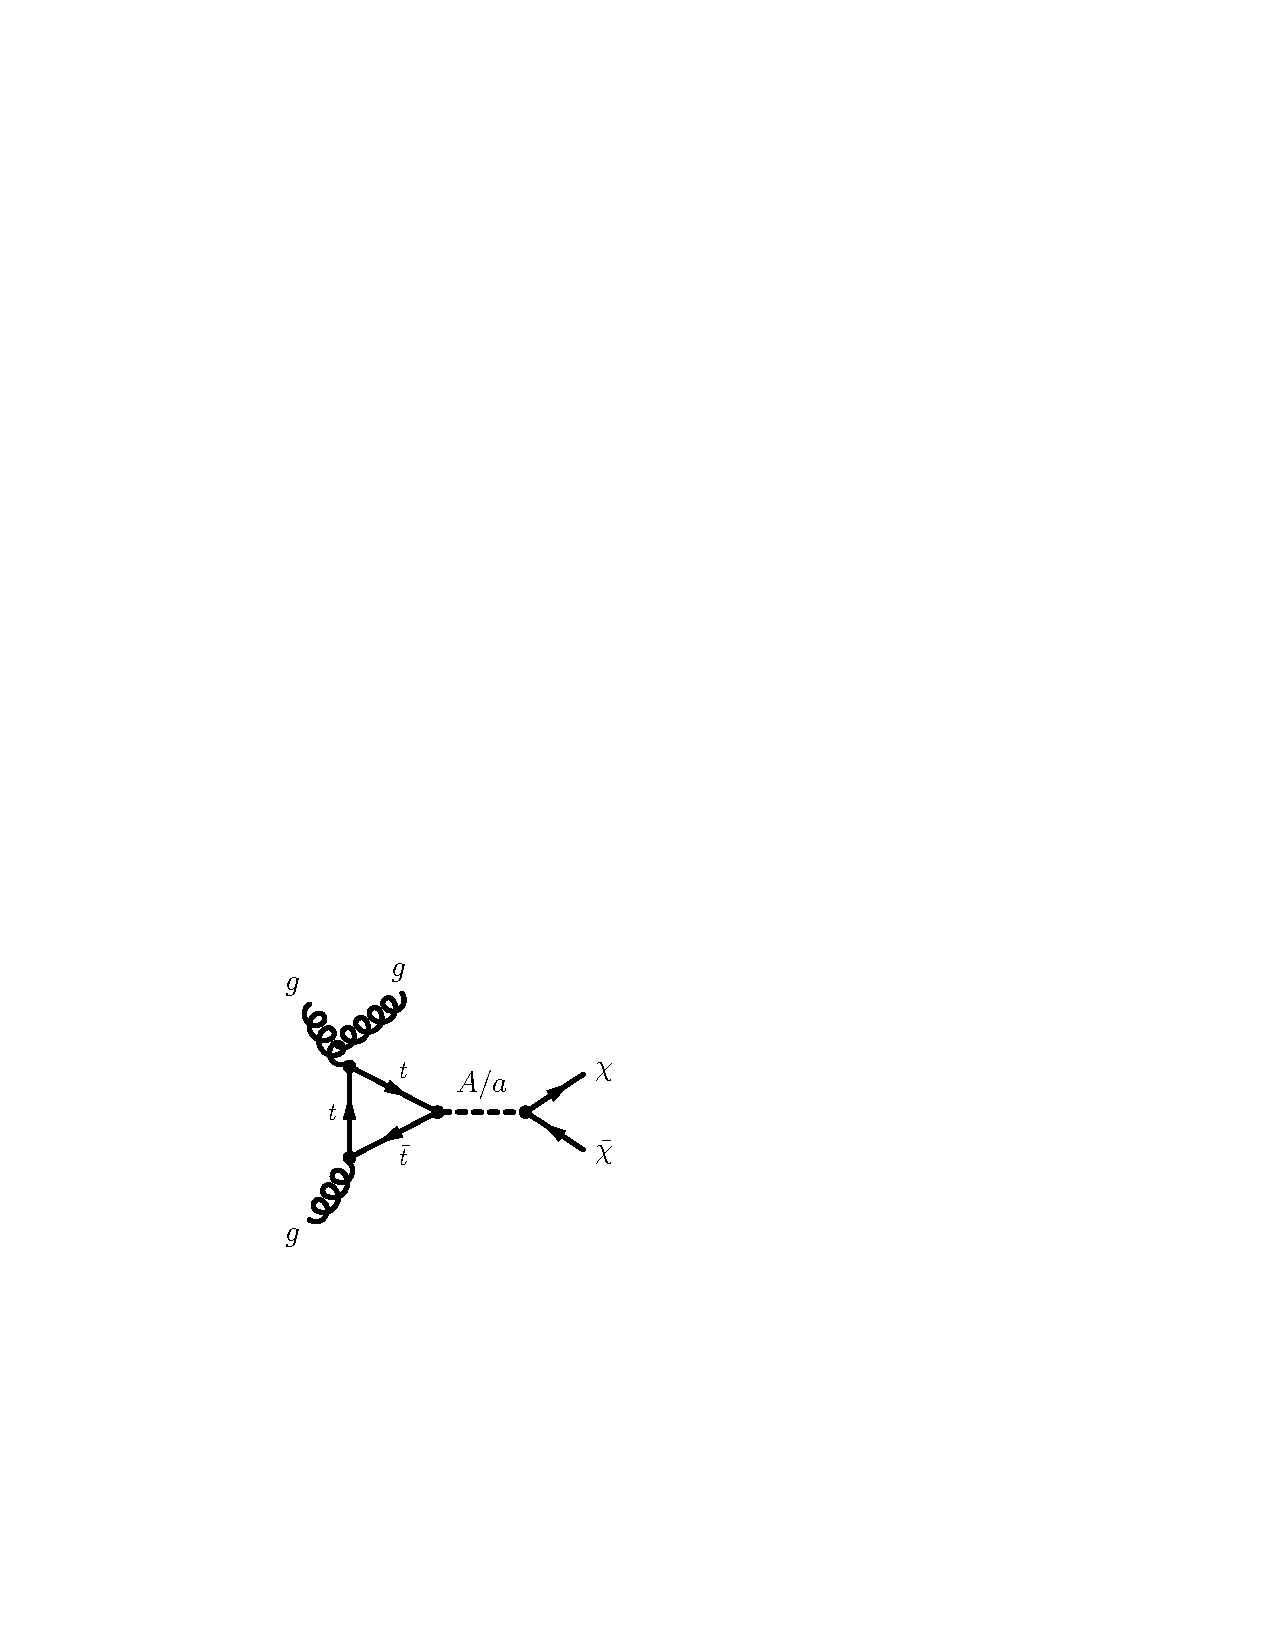
\includegraphics[width=0.6\textwidth]{figures/fig_01c.pdf}
        \vfill
        \caption{Gluon-gluon fusion}
        \label{subfig:metj-gg-fusion}
    \end{subfigure}
    \hfill
    \begin{subfigure}[3]{0.48\textwidth}
        \centering
        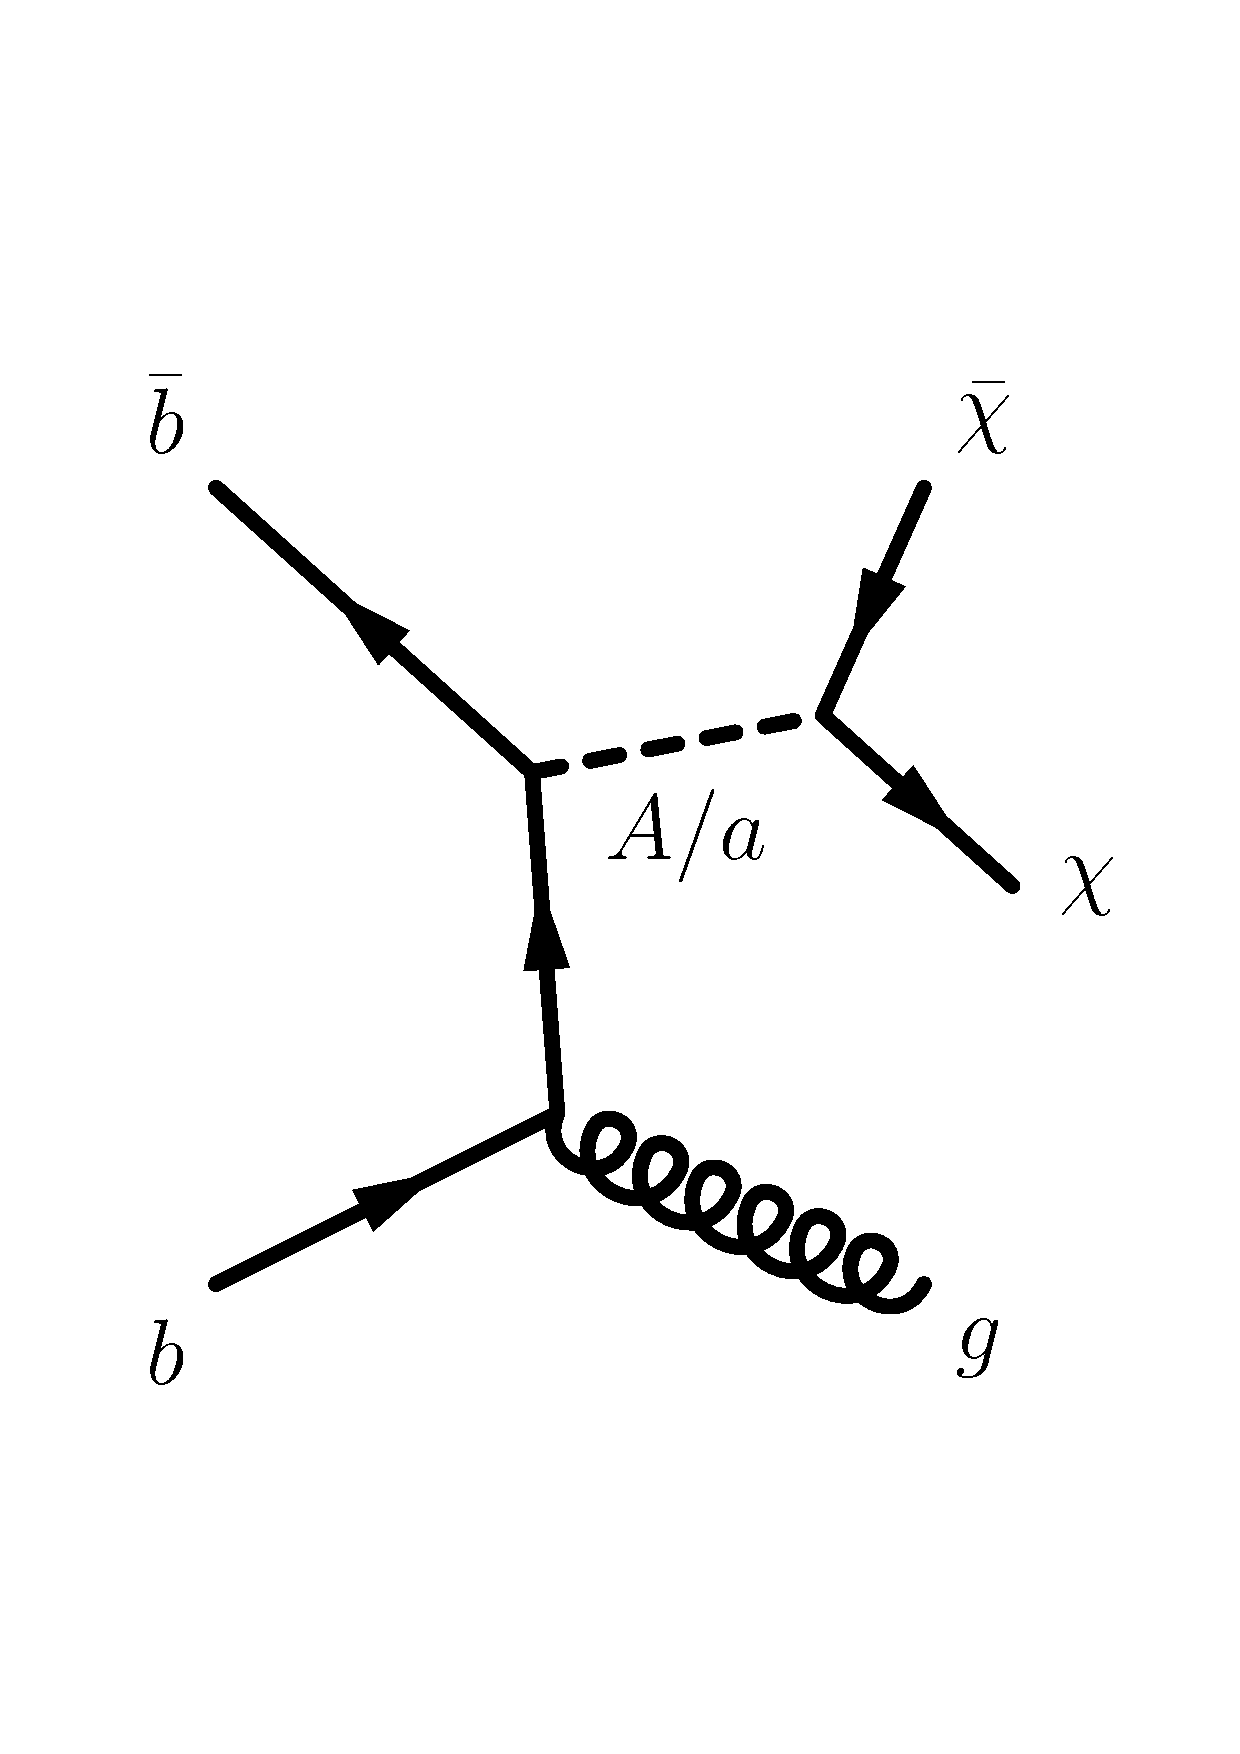
\includegraphics[width=0.6\textwidth]{figures/fig_02e.pdf}
        \caption{$b\bar{b}$-initiated}
        \label{subfig:metj-bb-associated}
    \end{subfigure}
    \caption{Production mechanisms and final state of the $\met+j$ signature, including gluon-gluon fusion production (a) and $b\bar{b}$-initiated production (b).}
    \label{fig:metj-signature}
\end{figure} 

This search targets final states containing a single jet and a large \met, which must satisfy $\met>200$ GeV to guarantee full \met trigger efficiency for all selected events \cite{EXOT-2018-06}. Events must contain a leading jet with $p_T>150$ GeV, $\abs{\eta} < 2.4$, up to three additional jets with $p_T>30$ GeV, $\abs{\eta} < 2.8$, and no leptons or photons. The azimuthal angular separation between the \met vector and each jet is required to meet $\Delta\phi(\met, jet) > 0.6$ for events with $200 < \met < 250$ GeV, and $\Delta\phi(\met, jet) > 0.4$ for those with $\met > 250$ GeV to reduce multijet backgrounds. 

Dominant SM backgrounds include $Z(\nu\nu)$ and $W(l\nu)$ production, in which the $W$ decays into a $\tau$-lepton which later decays hadronically, or other leptons that are undetected. Other contributions arise from $t\bar{t}$, single top quark, and diboson production, as well as non-collision and multijet backgrounds. These background contributions are estimated using a profile likelihood fit to the $p_T$ distribution of the system recoiling against the reconstructed jets in both signal and control regions.

In this combination, the search is reinterpreted in the context of \hdma, which is not considered in the original search. Several signal contributions to this signature are considered. In the low-\met region, the production of a pair of DM particles with a jet is the primary contribution at $\met< 500$ GeV $\ma\le 150$ GeV. Both $gg$-initiated and $bb$-initiated productions are considered, the latter of which is relevant at large $\tanb$. For larger \met and smaller $\ma$, the production of two pairs of DM particles via $h\rightarrow aa \rightarrow \chi\bar{\chi}\chi\bar{\chi}$ (figure \ref{fig:haaff-signature}) is the dominant process. Smaller contributions come from $\met+Z(q\bar{q})$ and $\met + h(b\bar{b})$ productions which the invisible decays of the SM Higgs boson are kinematically forbidden. Finally, minor contributions from $pp\rightarrow t\bar{t} +a$, and $pp\rightarrow tW+a$ are also present.

\subsection{\texorpdfstring{$\hinv$}{TEXT} signature}

The invisible decays of the SM Higgs boson represented by a \met associated to other visible signatures have been investigated in previous ATLAS publications and statistically combined in reference \cite{HIGG-2021-05}. The main production mechanisms include vector-boson fusion (VBF) \cite{EXOT-2020-11}, VBF with an emitted photon \cite{EXOT-2021-17}, gluon-gluon fusion \cite{EXOT-2018-06}, associated production with a vector boson \cite{HIGG-2018-26}, and associated production with a pair of top quarks \cite{SUSY-2019-12}. The results from Run 2 searches are combined statistically with constraints on invisible Higgs decays obtained from searches with up to 4.7 $\ifb$ of $pp$ collision data at $\sqrt{s}=7$ TeV and 20.3 $\ifb$ at $\sqrt{s}=8$ TeV \cite{HIGG-2015-03}. 

Among these searches, $\hinv$ from VBF production from Run 2 is the most sensitive and sets an observed limit of 0.145 and an expected limit of 0.103 at $95\%$ confidence level on the invisible branching ratio. Selected events are required to pass the \met trigger and have $\met>160$ GeV. They must also contain from two to four jets with $p_T>25$ GeV, among which the leading and sub-leading jets must have $p_T^{lead}>80$ GeV and $p_T^{sub-lead}>50$ GeV and be well separated in $\eta$. In addition, lepton and $b$-jet vetoes are applied to reduce $W+jets$ and top quark backgrounds. By partitioning the \met spectrum, the jet multiplicity, and jet-invariant masses, sixteen orthogonal signal regions are defined. Dominant background processes include $Z(\nu\nu)+jet$ and $W(l\nu)+jet$ production, the latter of which the charged lepton is undetected or misidentified. The backgrounds are estimated from control regions in the one-lepton and two-lepton channels. The multijet background is directly estimated from data. An upper limit on the $\hinv$ of $0.113\left(0.080^{+0.031}_{-0.022} \right)$ is observed (expected) at $95\%$ confidence level. 

\subsection{Additional searches using 36 \texorpdfstring{\ifb}{TEXT} of \texorpdfstring{$\sqrt{s}=13$}{TEXT} TeV \texorpdfstring{$pp$}{TEXT} collision data}

Three searches using 36 $\ifb$ of $\sqrt{s}=13$ TeV data are shown in this combination, the first of which targets $\met + Z(q\bar{q})$ signature \cite{EXOT-2016-23}. The final state contains a $\met>150$ GeV and a hadronically decaying vector boson reconstructed as a single large-$R$ jet with $p_T>250$ GeV in a boosted topology and two small-$R$ jets with $p_T>20$ GeV in a resolved topology. A lepton veto is applied in both cases. Signal regions are defined using the number of $b$-jets in the final state. The dominant backgrounds of $t\bar{t}$ and $W/Z+jets$ are estimated using a simultaneous fit to the \met distribution in he signal and control regions.

The second search targets a $\met+b\bar{b}$ signature. The final state contains at least two $b$-jets and $\met>180$ GeV \cite{SUSY-2016-18}. The irreducible background from $Z(\nu\nu)+b\bar{b}$ events separated from the signal events using the azimuthal separation between the $b$-jets and the \met. The results are extracted from a likelihood fit to the angular observable $\cos\theta*_{b\bar{b}} = \abs{\tanh\Delta\eta_{n\bar{b}}/2}$, in which $\Delta\eta_{n\bar{b}}$ is the difference in pseudorapidity between the $b$-jets.

The last group of searches targeting $\met+t\bar{t}$ and differing the the number of final-state leptons are included \cite{SUSY-2016-18}. A search in the final state where both $W$ bosons decay hadronically selects events with at least four energetic jets, of which at least two are $b$-jets, and a large \met. Several requirements on the invariant mass of the large-$R$ jets are applied to identify events with a boosted $W$ boson or top quark decay. The main backgrounds are $Z+jets$, $t\bar{t}$, and $t\bar{t}+Z$ production, constrained using dedicated control regions. A search in the one-lepton final state, resulting from a leptonically decaying $W$ boson, selects events with at least four energetic jets, at least one of which is a $b$-jet, an isolated lepton, and a large \met \cite{SUSY-2016-16}. They must also have at least one hadronic top candidate with invariant mass close to the top quark mass. The azimuthal separation between the lepton and \met and that between the jets and \met are used to suppress the background contamination in the signal regions. Dedicated control regions are used to estimate background processes involving top quarks.

\subsection{\texorpdfstring{$\htb$}{TEXT} signature}
\label{subsect:tbHtb}
The leading-order Feynman diagram for the target signature of this search is shown in figure \ref{fig:tbHtb-signature} \cite{HDBS-2018-51}. The charged Higgs boson is produced together with a top and a bottom quark, and subsequently decays into a top and a bottom quark, in which one top quark decays semi-leptonically. Events are preselected to contain exactly one electron or muon with $p_T>27$ GeV and at least five jets with $p_T>25$ GeV. At least three jets must be $b$-tagged to reduce large backgrounds from multijet production. Selected events are divided into four separate regions, namely $5j3b$, $5j\ge 4b$, $\ge 6j3b$, and $\ge 6j\ge 4b$, where $j$ and $b$ respectively stand for jets and $b$-jets. A neural network is trained to discriminate between signal and background, whose output distributions are used to extract the signal in data. 

Dominant backgrounds include $t\bar{t}+jets$, and single top quark production in the $Wt$ channel. The former is divided into $t\bar{t}+\mathrm{light}$, $t\bar{t}+\ge 1b$, and $t\bar{t}+\ge 1c$. These along with other minor backgrounds are model using MC simulation and corrections obtained from an additional $\ge 5j2b$ region via a reweighting procedure \cite{ATL-PHYS-PUB-2018-009, TOPQ-2018-18}. After the reweighting, the $t\bar{t}+\ge 1b$ and $t\bar{t}+ \ge 1c$ normalizations factors are extracted from the fit to data. 

\begin{figure}[h!]
    \centering
    \begin{subfigure}[3]{0.48\textwidth}
        \centering
        \begin{tikzpicture}
          \begin{feynman}
            \vertex (h) at (0,0);
            \vertex (tgp) at (-0.3, 1) ;
            \vertex (bgp) at (-0.3, -1) ;
            \vertex (gt) at (-1.8, 1.2) {$g$};
            \vertex (gb) at (-1.8, -1.2) {$g$};
            \vertex (t) at (1.4, 1.2) {$t$} ;
            \vertex (b) at (1.4, -1.2) {$\bar{b}$};
            \vertex (htb) at (1.2, 0) ;
            \vertex (th) at (2.1, 0.6) {$\bar{t}$};
            \vertex (bh) at (2.1, -0.6) {$b$};
            \diagram[] {
                (h) -- [fermion] (tgp),
                (bgp) -- [fermion] (h),
                (gt) -- [gluon] (tgp),
                (gb) -- [gluon] (bgp),
                (tgp) -- [fermion] (t),
                (b) -- [fermion] (bgp),
                (h) -- [scalar, edge label=\(H^{-}\)] (htb),
                (htb) -- [anti fermion] (th),
                (bh) -- [anti fermion] (htb),
            };
          \end{feynman}
        \end{tikzpicture}
    \end{subfigure}
    \caption{Production mechanisms and final state of the $\htb$ signature.}
    \label{fig:tbHtb-signature}
\end{figure} 

\subsection{\texorpdfstring{$t\bar{t}t\bar{t}$}{TEXT} signature}

\begin{figure}[h!]
    \centering
    \begin{subfigure}[3]{0.48\textwidth}
        \centering
        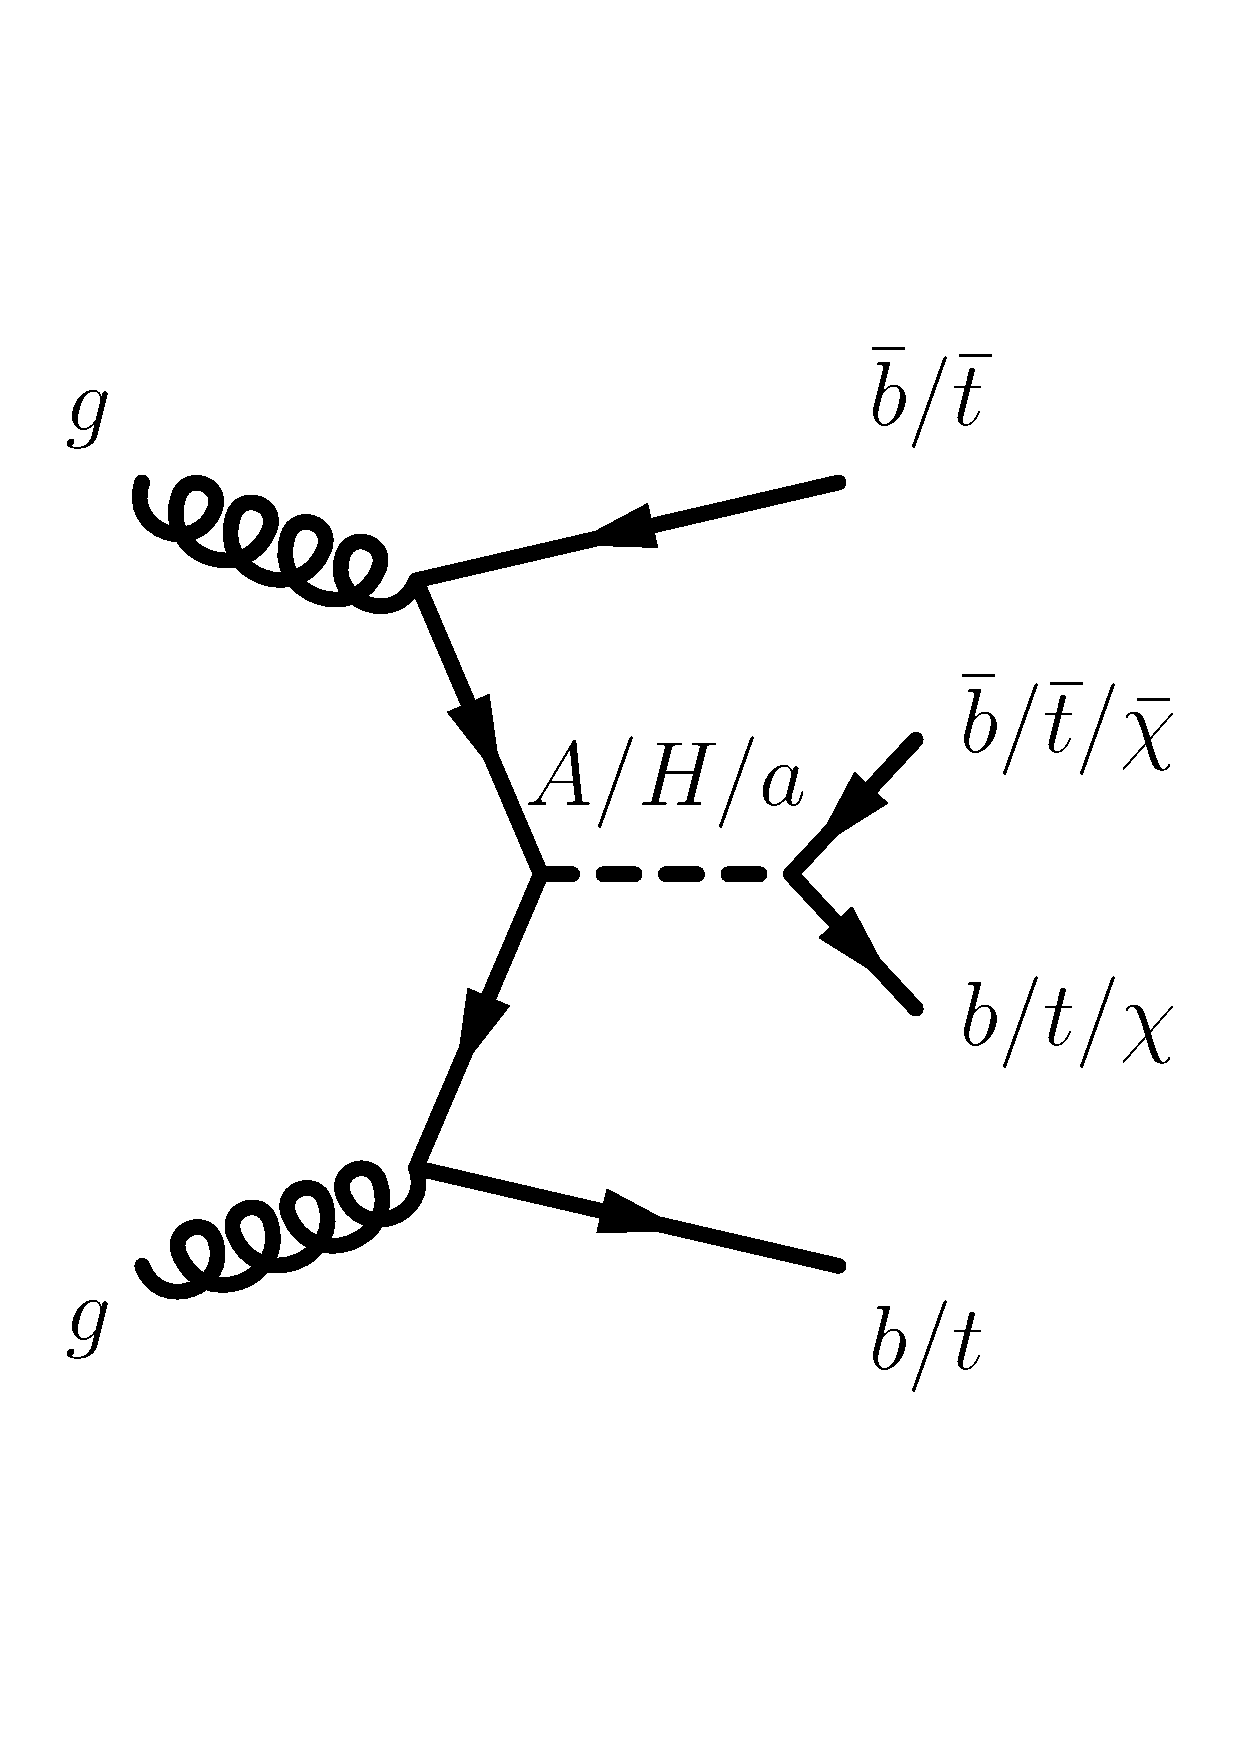
\includegraphics[width=0.7\textwidth]{figures/fig_01e.pdf}
    \end{subfigure}
    \caption{Production mechanisms and final state of the $t\bar{t}t\bar{t}$, $\met+b\bar{b}$, and $\met+t\bar{t}$ signatures.}
    \label{fig:tttt-signature}
\end{figure} 

The targeted signature of this search, shown in figure \ref{fig:tttt-signature}, is a $t\bar{t}$-associated production of a heavy scalar or pseudo-scalar Higgs boson in the \hdma, which then decays into a pair of top quarks\cite{EXOT-2019-26}. The final state contains 2 pairs of top quarks, decaying into either two leptons with the same-sign electric charge or at least three leptons, both with high jet multiplicity. These leptons include electrons or muons from leptonic $\tau$ decay, and are required to have $p_T>28$ GeV. A baseline signal region is defined by requiring six jets with $p_T>25$ GeV, among which at least two are $b$-tagged, and a scalar sum of the all transverse momenta of jets and leptons $H_T>500$ GeV. First, a BDT is trained to separate SM $t\bar{t}t\bar{t}$ production and background processes using event-level inputs. A second BDT, designated BSM mass-parametrised BDT (BSM pBDT), is then trained to discriminate between BSM $t\bar{t}t\bar{t}$ events and all background. It is parametrised as a function of the mass of the heavy Higgs boson by introducing the mass as an input in the training \cite{Baldi:2016fzo}.

The major irreducible backgrounds arise from the top quark pair production with a boson and jets ($t\bar{t}+W+jets$, $t\bar{t}+Z+jets$, and $t\bar{t}+h+jets$). These contributions are estimated using MC simulations with data-driven corrections for $t\bar{t}+W+jets$. Minor, irreducible backgrounds originate mostly from $t\bar{t}+jets$ and $tW+jets$ production with misidentified charge, fake and non-prompt leptons, which are estimated from data using dedicated control regions.

\subsection{Exotic Higgs boson decays \texorpdfstring{$h\rightarrow aa\rightarrow f\bar{f}f'\bar{f}'$}{TEXT}}

\begin{figure}[h!]
    \centering
    \begin{subfigure}[3]{0.48\textwidth}
        \centering
        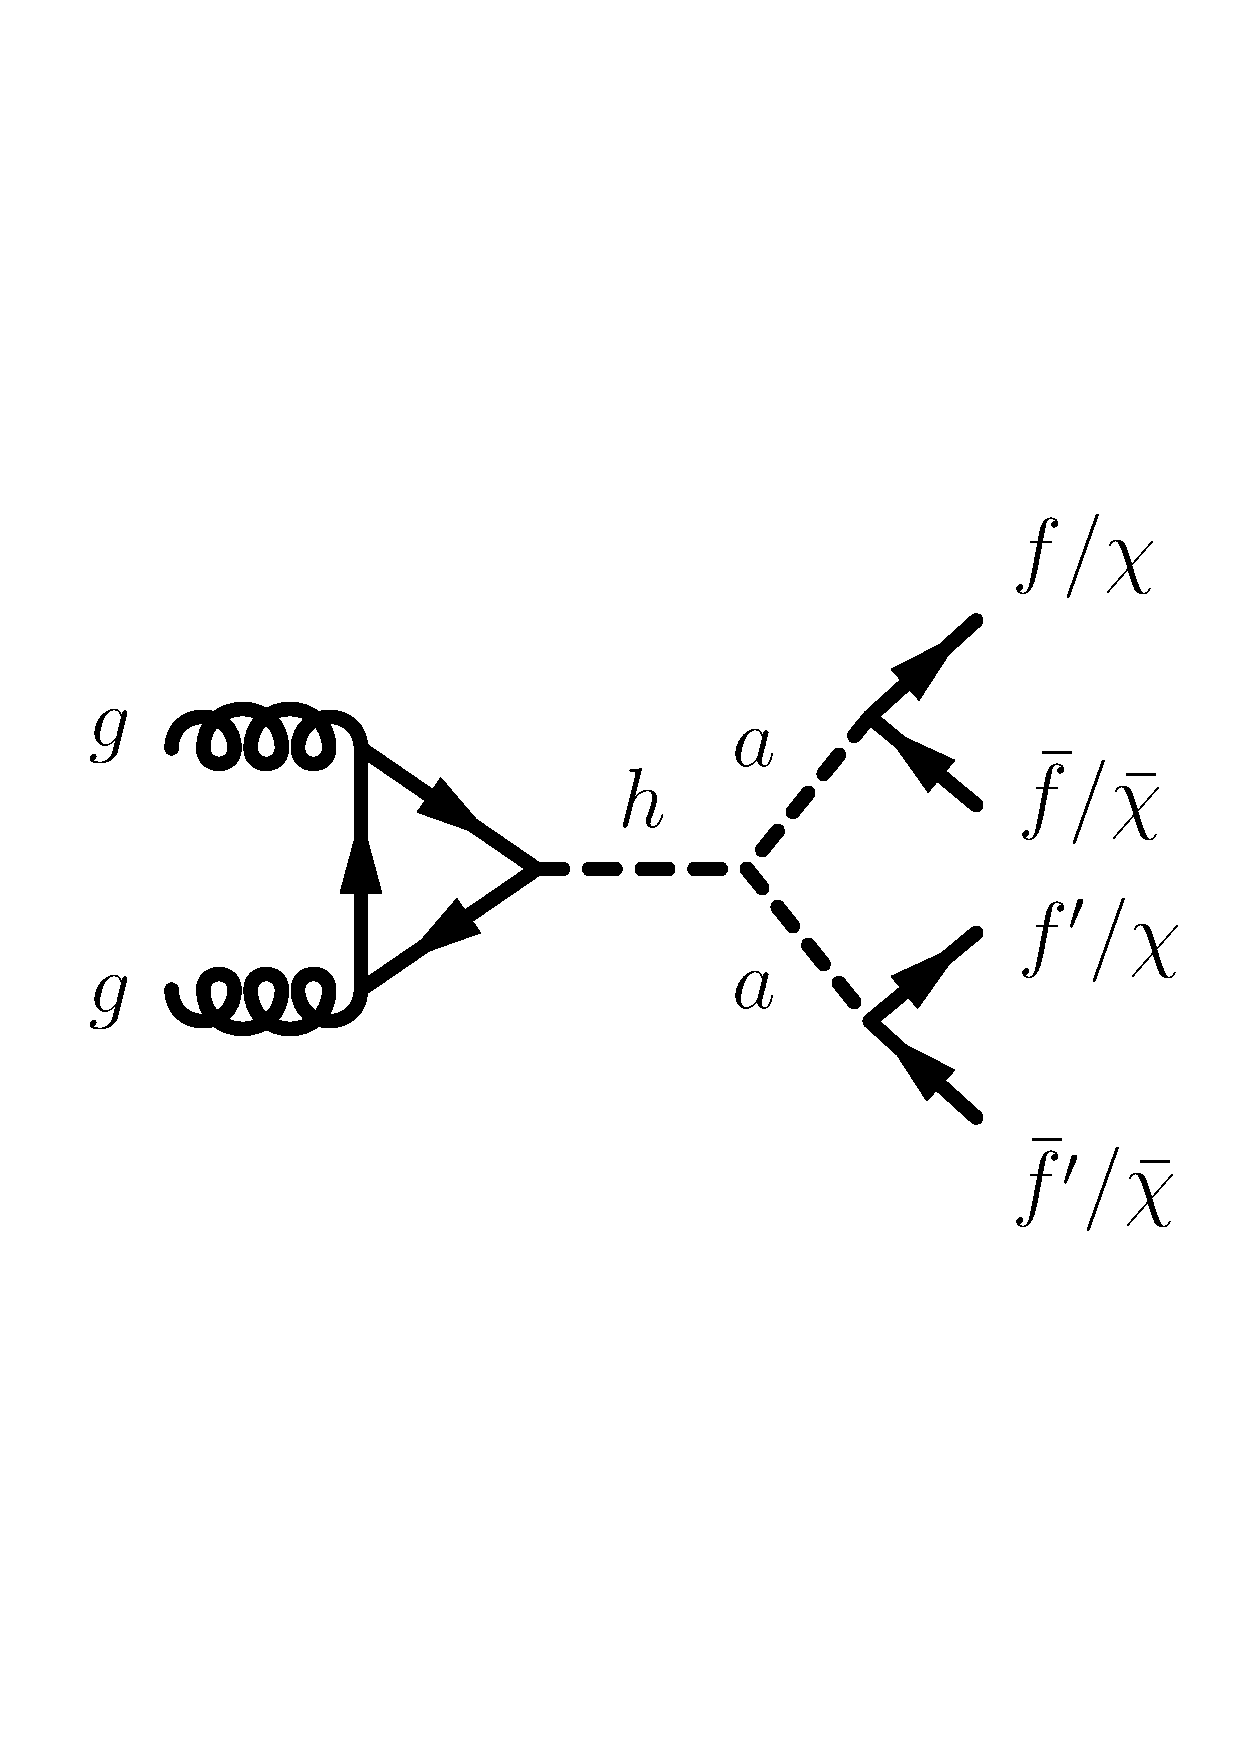
\includegraphics[width=0.7\textwidth]{figures/fig_01g.pdf}
    \end{subfigure}
    \caption{Production mechanisms and final state of the $h\rightarrow aa\rightarrow f\bar{f}f'\bar{f}'$ signature.}
    \label{fig:haaff-signature}
\end{figure} 

This set of searches target the decays of the SM Higgs boson into a pair of light pseudo-scalar particles $aa$, which then decay into four fermions, as illustrated in figure \ref{fig:haaff-signature}. Depending on the type of fermion present in the final state, the searches provide sensitivity to different pseudo-scalar mass ranges.

The first search uses 139 $\ifb$ of $\sqrt{s}=13$ TeV $pp$ collision data, and targets the $b\bar{b}\mu^+\mu^-$ final state \cite{HDBS-2021-03}. It is sensitive to pseudo-scalar mass in the range $16<\ma<62$ GeV. The variable of interest is the dimuon invariant mass, chosen to probe for a resonant enhancement over the SM expectation. The dominant background is the Drell-Yan dimuon process together with $b$ quarks and SM $t\bar{t}$ production where both $W$ bosons from the top quarks decay into a muon and a neutrino. 

A second search using 36 $\ifb$ of $\sqrt{s}=13$ TeV $pp$ collision data targeting $b\bar{b}b\bar{b}$ final state provides sensitivity in the mass range $20<\ma<60$ GeV \cite{HIGG-2017-05}. The Higgs boson is produced in associated with a leptonically decaying $W$ boson (one-lepton channel) or $Z$ boson (two-lepton channel). Signal-background separation is performed with a BDT trained using event-level kinematic variables, notably the reconstructed pseudo-scalar masses. The dominant background process in the one-lepton channel is $t\bar{t}$ production with additional jets, and $Z+jet$ in the two-lepton channel. The BDT output distribution is used as the observable of interest in the final likelihood fit. This search is optimized for the resolved topology of the $b\bar{b}$ dijet system, i.e. they are reconstructed as two small-$R$ jets. 

A third search on 20.3 $\ifb$ of $\sqrt{s}=8$ TeV $pp$ collision targeting $\mu^+\mu^-\tau^+\tau^-$ probes the mass range $3.7<\ma<50$ GeV. It probes resonant enhancement in the dimuon invariant mass spectrum \cite{HIGG-2014-02}.

The last searches considered in this combination target final states with four charged leptons ($l=e,\,\mu$) on 36 $\ifb$ and 139 $\ifb$ of $\sqrt{s}=13$ TeV \cite{EXOT-2016-22, HDBS-2018-55}. They probe two orthogonal pseudo-scalar mass regions, namely a low-mass region covering $1<\ma<15$ GeV range, excluding the mass ranges around the $J/\psi$ and the $\Upsilon$ resonances, and a high-mass region covering $15<\ma<60$ GeV. The high-mass range is insensitive to \thdma and therefore excluded from this combination. The final states containing at least four muons are exclusively considered thanks to their large branching ratio and the large selection efficiency of isolated muons relative to that of isolated electrons. The dominant background process is $ZZ^*\rightarrow \mu^+\mu^-\mu^+\mu^-$ and $h\rightarrow ZZ^*\rightarrow \mu^+\mu^-\mu^+\mu^-$. The observable of interest is the average dimuon invariant mass $\expval{m_{\mu^+\mu^-}} = (m_{12} + m_{34})/2$, in which the pairing is done to minimize the dimuon invariant mass difference. 

Model-independent upper limit on the branching ratio of the $h\rightarrow aa \rightarrow 4f$ are obtained. The upper limit is used directly to exclude parameter regions in the \thdma based on the predicted $h\rightarrow aa \rightarrow 4f$ branching ratio for each point considered in the benchmark scenarios in the previous section. 


\section{Systematic uncertainties}
\label{sect:systematic-uncertainties}

Systematic and statistical uncertainties depend on event selection, the considered phase space, and the background estimation strategy. Systematic uncertainties may be of experimental or theoretical origin. In general, experimental uncertainties may include uncertainties in the absolute jet energy scales and resolutions, jet quality requirements, pile-up corrections, $b$-jet identification efficiencies, and the soft contributions to \met. Uncertainties in lepton identification and reconstruction efficiencies, energy/momentum scale and resolution are considered from events with selected or vetoed leptons. Uncertainties due to the finite size of the background MC samples and others related to the modelling of the background processes are also included in the analyses. A luminosity uncertainty of 1.7\% is applied to backgrounds derived purely from MC simulation \cite{ATLAS-CONF-2019-021}. 

Theoretical uncertainties on the production cross-section or on the signal acceptance affect signal modelling. They include uncertainties related to the PDF and are evaluated following the PDF4LHC recommendations \cite{Butterworth:2015oua}. Other uncertainties pertain to the choice of renormalization and factorization scales. They are derived by varying independently such scales by a factor of 2.0 and 0.5 relative to the nominal values used for MC generation. In addition, for signatures entering the statistical combination, uncertainties in the modelling of initial- and final-state radiation and multi-parton interactions are taken into account. 

\section{Statistical combination of results}
\label{sect:stat}
Three \thdma signatures are selected to enter a statistical combination, namely $\monohbb$, $\monozll$, and $tbH^{\pm}tb$. They cover complementary regions of the model parameter space, and are the most constraining signatures of those described in \ref{sect:exp-signatures}. These factors simplify the statistical treatment and enhance the sensitivity to the \thdma signal.

These input analyses are statistically independent, due to their event selection. The $\monozll$ analysis vetoes events with $b$-jets, whereas the other analyses require the presence of at least two jets. The $\htb$ targets final states with a charged lepton, while $\monohbb$ vetoes the presence thereof. Therefore, the signal region of these analyses are completely separated. A small event overlap ($<1\%$) is observed between $\htb$ signal region and the leptonic control region of the $\monohbb$ analysis, but has no impact on the combination.

\subsection{Statistical analysis}

To statistically combine the results of these analyses, a combined likelihood function is constructed and the corresponding profile likelihood ratio maximized \cite{Cowan:2010js}. The common parameter of interest (POI) is the signal strength of a \thdma signal at a particular point in the parameter space, defined as the ratio of the observed number of signal event to the signal cross-section times branching ratio. Systematic uncertainties are introduced to the likelihood as constrained nuisance parameters (NPs), denoted by $\theta_{\mu}$, and modelled by Gaussian, Poisson, or Log-normal probability density function. Background normalization factors, denoted by $\lambda_{\mu}$, are floated without constraints in the fit to estimate the background components in their corresponding control regions. The subscript $\mu$ on these parameter is in anticipation of their dependence on the best-fit signal strength.

The combined likelihood is given by
\begin{equation}
    \label{4.13}
    L(\mathrm{data}|\mu,\lambda_{\mu},\theta_{\mu})= \prod_{c=1}^{N_{cats}} {L}_c(\mathrm{data}|\mu, \lambda_{\mu}, \theta_{\mu}) \prod_{k=1}^{N_{cons}} {F}(\Tilde{\theta}_{\mu, k}|\theta_{\mu, k}),
\end{equation}
where $N_{cats}$ is the number of categories, $c$ the index of the event category, $N_{cons}$ the number of constrained NPs, $k$ the index of the NP, $\Tilde{\theta}_{\mu, k}$ the global observable corresponding to $\theta_k$, and $F$ the constraining probability distribution function corresponding to the type of uncertainty. 
The likelihood of observing $m_c$ events in category $c$ is
\begin{equation}
    \label{chap:phys-anal:14}
    L_c(data|\mu, \lambda_{\mu}, \theta_{\mu}) = \frac{n_c^{m_c}e^{-n_c}}{m_c!}, \quad n_c = \mu s_c(\theta_{\mu}) + \lambda_{\mu}b_c(\theta_{\mu}),
\end{equation}
in which $s_c$ and $b_c$ are expected signal and background yields.
The likelihood can be globally maximized or conditional on a particular value of $\mu$.

The $95\%$ confidence level (CL) limits are obtained by the CLs frequentist formalism \cite{ReadCLs} using the profile likelihood ratio test statistics ($q_{\mu}$)\cite{Cowan:2010js}, defined as 
\begin{equation}
    \label{4.14}
    q_{\mu} = \begin{cases} 
     -2\ln\frac{L(\mathrm{data}|\mu,\hat{\hat{\lambda}}_{\mu},\hat{\hat{\theta}}_{\mu})}{L(\mathrm{data}|0,\hat{\hat{\lambda}}_{0},\hat{\hat{\theta}}_{0})}\quad &  \hat{\mu}<0, \\
        -2\ln\frac{L(\mathrm{data}|\mu,\hat{\hat{\lambda}}_{\mu},\hat{\hat{\theta}}_{\mu})}{L(\mathrm{data}|\hat{\mu},\hat{\lambda}_{\mu},\hat{\theta}_{\mu})}\quad & 0\le \hat{\mu}<\mu, \\
        0 \quad & \hat{\mu} > \mu
    \end{cases}
\end{equation}
where the numerator is the likelihood maximized for a given fixed value of $\mu$, and the denominator is the globally maximized likelihood. The single-hat quantities denote the global optimum values, while the double-hat quantities denote the optima at $\mu$, i.e. a function of $\mu$.
The confidence level is determined from the $p$-values of the $b$-only hypothesis and the different $s+b$ hypotheses,
\beq
\label{chap:phys-ana:15}
\mathrm{CL}_s = \frac{p_{s+b}}{1-p_{b}}.
\eeq
Each signal hypothesis corresponds to a particular point in the parameter space.
The $p$-value of the null hypothesis $p_b$ and the signal hypothesis is obtained by setting $q_0=0$ and evaluating $q_1$ in equation \eqref{4.14} respectively and integrating over the corresponding sampling distribution \cite{Cowan:2010js}.
A signal model, i.e. a parameter point, is said to be excluded at $95\%$ CL when $CL_s<0.05$. 


\subsection{Uncertainties and their correlations}

Each of the three analyses treats a particular set of uncertainties. 
Often times, more than one analysis estimate the same systematic uncertainty, in which case it is correlated in the combination. 
This section describes this treatment. 
Most experimental uncertainties are correlated across search channels, namely they are modelled using the same observable in the combined likelihood. 
They include uncertainties related to the reconstruction of physics objects, the integrated luminosity, and pile-up modelling. 
Physics object uncertainties include those from electrons, muons, and the jet energy response. 
Uncertainties from $b$-jet identification depend on $b$-tagging algorithm and working point, which vary across the analyses. 
As a result, they are not correlated. 
Finally, several experimental systematic uncertainties are moderately constrained in a particular analysis, and hence not correlated to avoid phase-space biases. 
Different assumptions on the correlation of uncertainties related to jet, \met, and $b$-jet identification, and other moderately constrained uncertainties are tested to gauge their impact on the observed exclusions, and found to have negligible impact. 

Uncertainties on signal simulation and background modelling are assessed for each analysis. To each final state is dedicated a separate signal simulation, as they often probe different kinematic regions of the phase space. The theoretical uncertainties are found to be small and are considered to be uncorrelated. Uncertainties pertaining to background modelling are considered correlated amongst the analyses, motivated by their different sources of leading background, different probed kinematic phase space, as well as different methods of background estimation.

\subsection{The impact of uncertainties}

Different \thdma parameter values correspond to different signal kinematics and sensitivity delivered by each analysis, and thus see different levels of impact from uncertainties on the combined signal strength. As an example, the contributions to the uncertainty of the best fit signal strength from statistical and systematic uncertainties are shown in table \ref{tab:uncertainty-contribution} for a parameter point at $\ma=450$ GeV, $m_H=800$ GeV, $\tanb=1.0$, and $\sint=0.35$. This signal is not excluded by any single input analysis, but is excluded by the combination. The statistical uncertainty is slightly smaller than the systematic counterpart, which is broken into three categories: theoretical, experimental, and MC statistical uncertainties. The impact of each category is estimated by fixing the uncertainties in that category in a fit, and subtracting the resulting uncertainty in the signal strength from the total in quadrature. Theoretical uncertainties arise mainly from uncertainties in background modelling and are slight smaller than experimental ones. Among the experimental uncertainties originating from reconstructed physics objects, those from jet and \met make the largest contributions. 

For each input analysis, the most important uncertainties also make the largest contribution to the combined uncertainty. For background modelling, the largest components are $ZZ$ modelling from $\monozll$, $t\bar{t}$ uncertainties from $\met+h(bb)$, and uncertainties from $t\bar{t}$ production with additional $b$ quarks from $\htb$. Among experimental systematic uncertainties, the largest sources are lepton systematic uncertainties from $\monozll$, uncertainties related to jets and \met from $\met+h(bb)$, and those related to $b$-jet identification from $\htb$.

\begin{table}
    \centering
    \begin{tabular}{lllr}
    \hline\hline
        \multicolumn{3}{l}{Uncertainty source} & $\Delta\mu\cdot 100$\\
        \hline
        \multicolumn{3}{l}{Statistical uncertainty}  & $25.0$ \\
        \hline
         \multicolumn{3}{l}{Systematic uncertainty}  & $27.6$ \\
         &  \multicolumn{2}{l}{Theory uncertainties}  &  $16.2$\\
         & & Signal modelling & $2.8$ \\
         & & Background modelling & $15.9$ \\
         & \multicolumn{2}{l}{Experimental uncertainties (excl. MC stat.)} & $18.8$ \\
         & & Luminosity, pile-up & $3.9$ \\ 
         & & Jets, \met & $12.3$ \\
         & & Identification of $b$-jets & $9.1$ \\
         & & Electrons, muons & $6.1$ \\
         & \multicolumn{2}{l}{MC statistical uncertainty} & $9.3$ \\
         \hline
         \multicolumn{3}{l}{Total uncertainty} & $37.2$ \\
    \hline\hline
    \end{tabular}
    \caption{Impact from different sources of uncertainties on the best-fit signal strength express in $\Delta\mu$ on the signal at $(\mA=800\, \mathrm{GeV}, \ma=450 \, \mathrm{GeV}, \tanb=1, \sint=0.35)$, estimated by fixing the corresponding NPs to their best-fit values, and subtracting the resulting uncertainty from the total uncertainty in quadrature. The statistical uncertainty component is obtained by fixing all NPs except the floating background normalization factors, and quantifies the impact of the limit data yields in the signal and control regions. The total uncertainty is not the quadratic sum of the individual contribution due to correlations between systematic uncertainties \cite{2hdma_comb}.}
    \label{tab:uncertainty-contribution}
\end{table}

\section{Results on combined constraints on the \thdma}
\label{sect:combined-result}
A summary of combined constraints on \thdma across all benchmark scenarios introduced in section \ref{sect:benchmark-scenarios} is presented in this section. 

\subsection{Scenario 1: \texorpdfstring{$\ma-\mA$}{TEXT} planes}
Figure \ref{fig:result-ma-mA-scan} shows the exclusion contours from the $\ma-\mA$ scans with the 2HDM mixing angle fixed to $\sint=0.35$ in \ref{fig:result-ma-mA-scan-a} and \ref{fig:result-ma-mA-scan-c}, and $\sint=0.7$ in \ref{fig:result-ma-mA-scan-b} and \ref{fig:result-ma-mA-scan-d}. These choices of parameters correspond to benchmark scenarios 1a and 1b in section \ref{sect:benchmark-scenarios}. The combined exclusion contours are shown along with those of the three individual channels entering the statistical combination in \ref{fig:result-ma-mA-scan-a} and \ref{fig:result-ma-mA-scan-b}, and with the remaining channels in \ref{fig:result-ma-mA-scan-b} and \ref{fig:result-ma-mA-scan-d}. Over the two benchmark parameter planes, the $\monozll$ and $\monohbb$ drive the sensitivity across a large region, due primarily to the resonant production of the scalar and pseudo-scalar according to the diagram in figures \ref{subfig:zll-gg-fusion-res} and \ref{subfig:hbb-gg-fusion-res}. Their sensitivity varies widely with the pseudo-scalar Higgs boson and the mediator masses. At $\sint=0.35$ and in the region where $\monozll$ and $\monohbb$ dominate, all pseudo-scalar mass is excluded up to a maximum $\ma=560$ GeV for $\mA=1.2$ TeV, while for $\ma=1.5$ GeV, all pseudo-scalar Higgs mass is excluded up to $\mA=1.55$ TeV. At $\sint=0.7$, all pseudo-scalar mass is excluded up to a maximum $\ma=550$ GeV for $\mA=1$ TeV, while for $\ma=400$ GeV, all pseudo-scalar Higgs mass is excluded up to $\mA=1.2$ TeV. For both choices of $\sint$, the $\monozll$ contour reaches closer to the $\mA=\ma$ limit than that of $\monohbb$, because the former can probe lower \met values, whereas the latter is sensitive at higher \met due to the presence of a \met trigger in its selection and the mass difference between the $Z$ and the Higgs bosons. In addition, the exclusion power of $\monohbb$ is increased relative to $\monozll$ at high $\mA$ and low $\ma$, because of an increase in the cross-section of the non-resonant $a^*\rightarrow ah$ process, without resonant $A$ production, which has no equivalence in the latter's signature.

\begin{figure}[h!]
    \centering
    \begin{subfigure}[2]{0.495\textwidth}
        \centering
        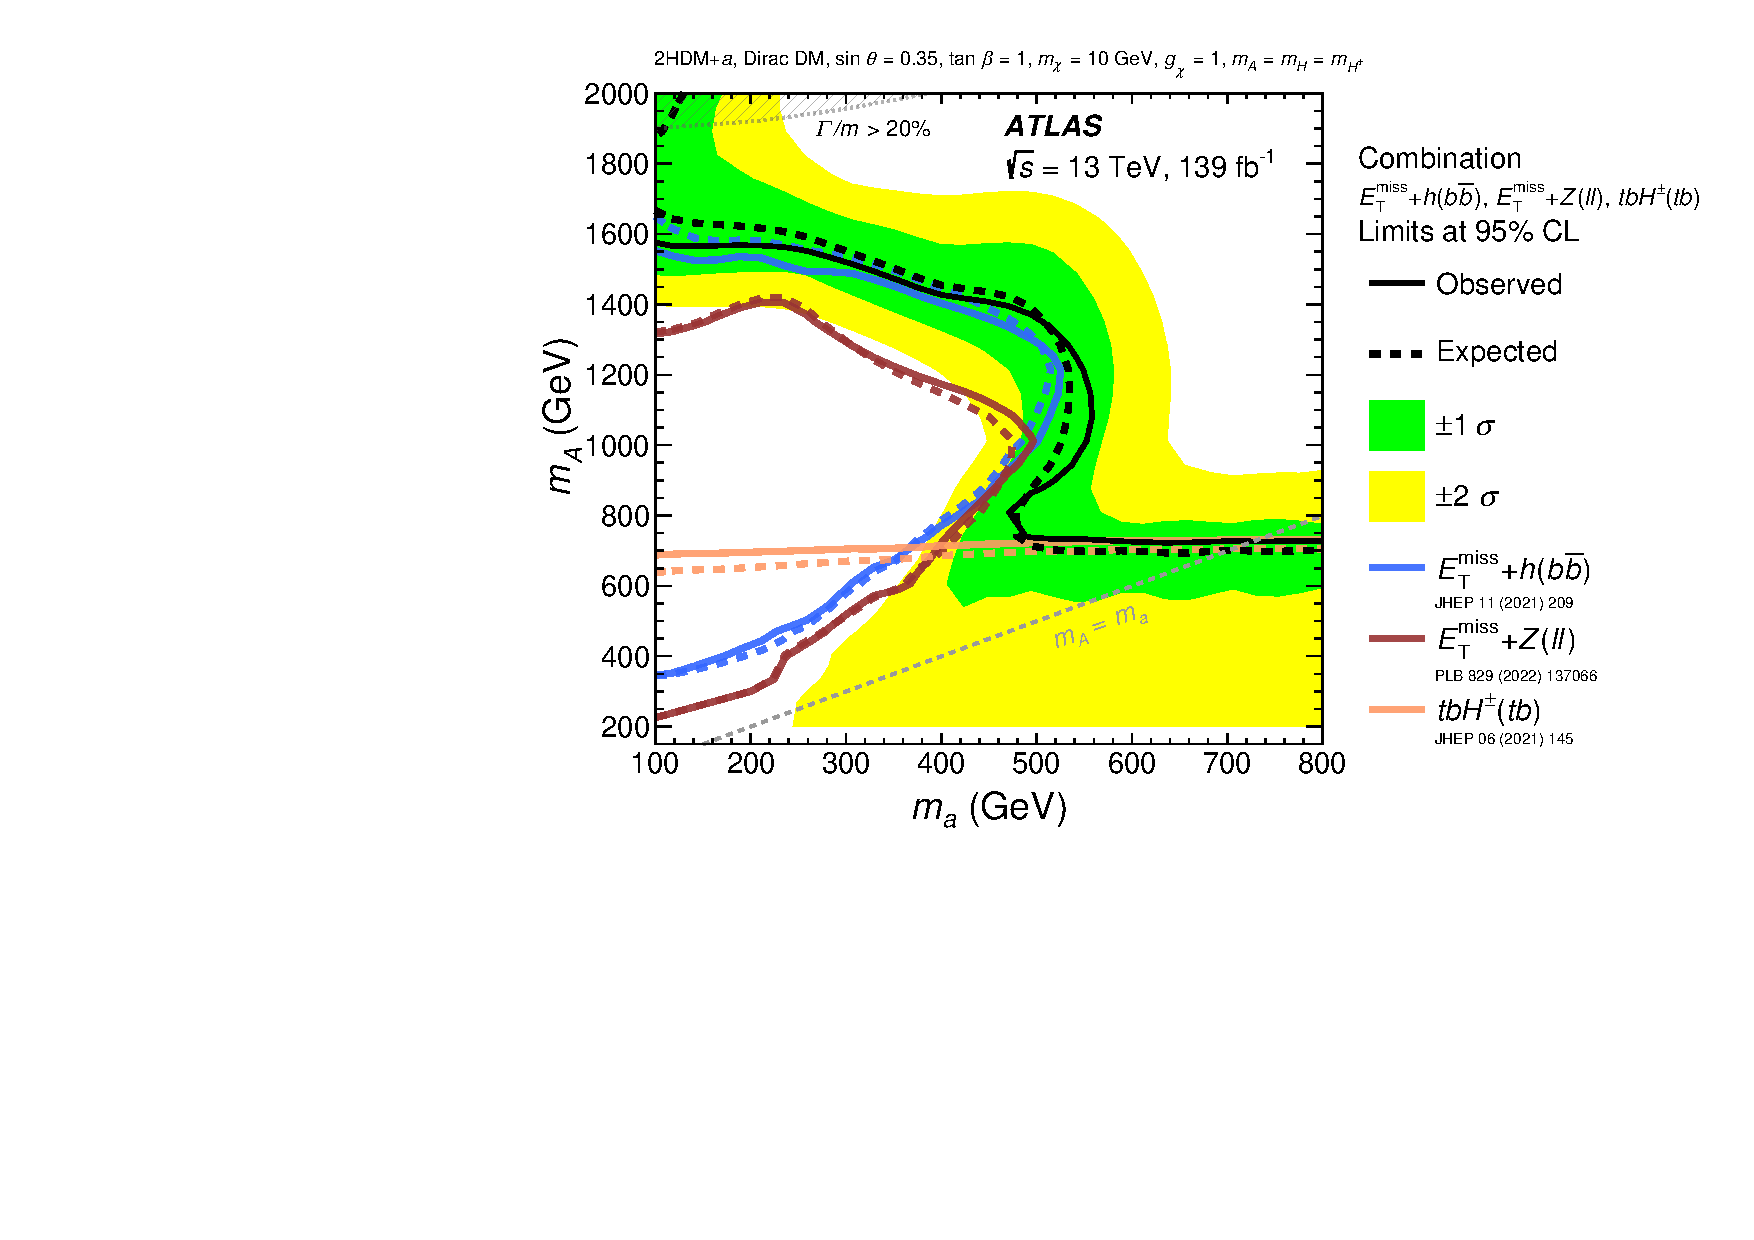
\includegraphics[width=\linewidth]{figures/fig_04a.pdf}
        \caption{}
        \label{fig:result-ma-mA-scan-a}
    \end{subfigure}
    \begin{subfigure}[2]{0.495\textwidth}
        \centering
        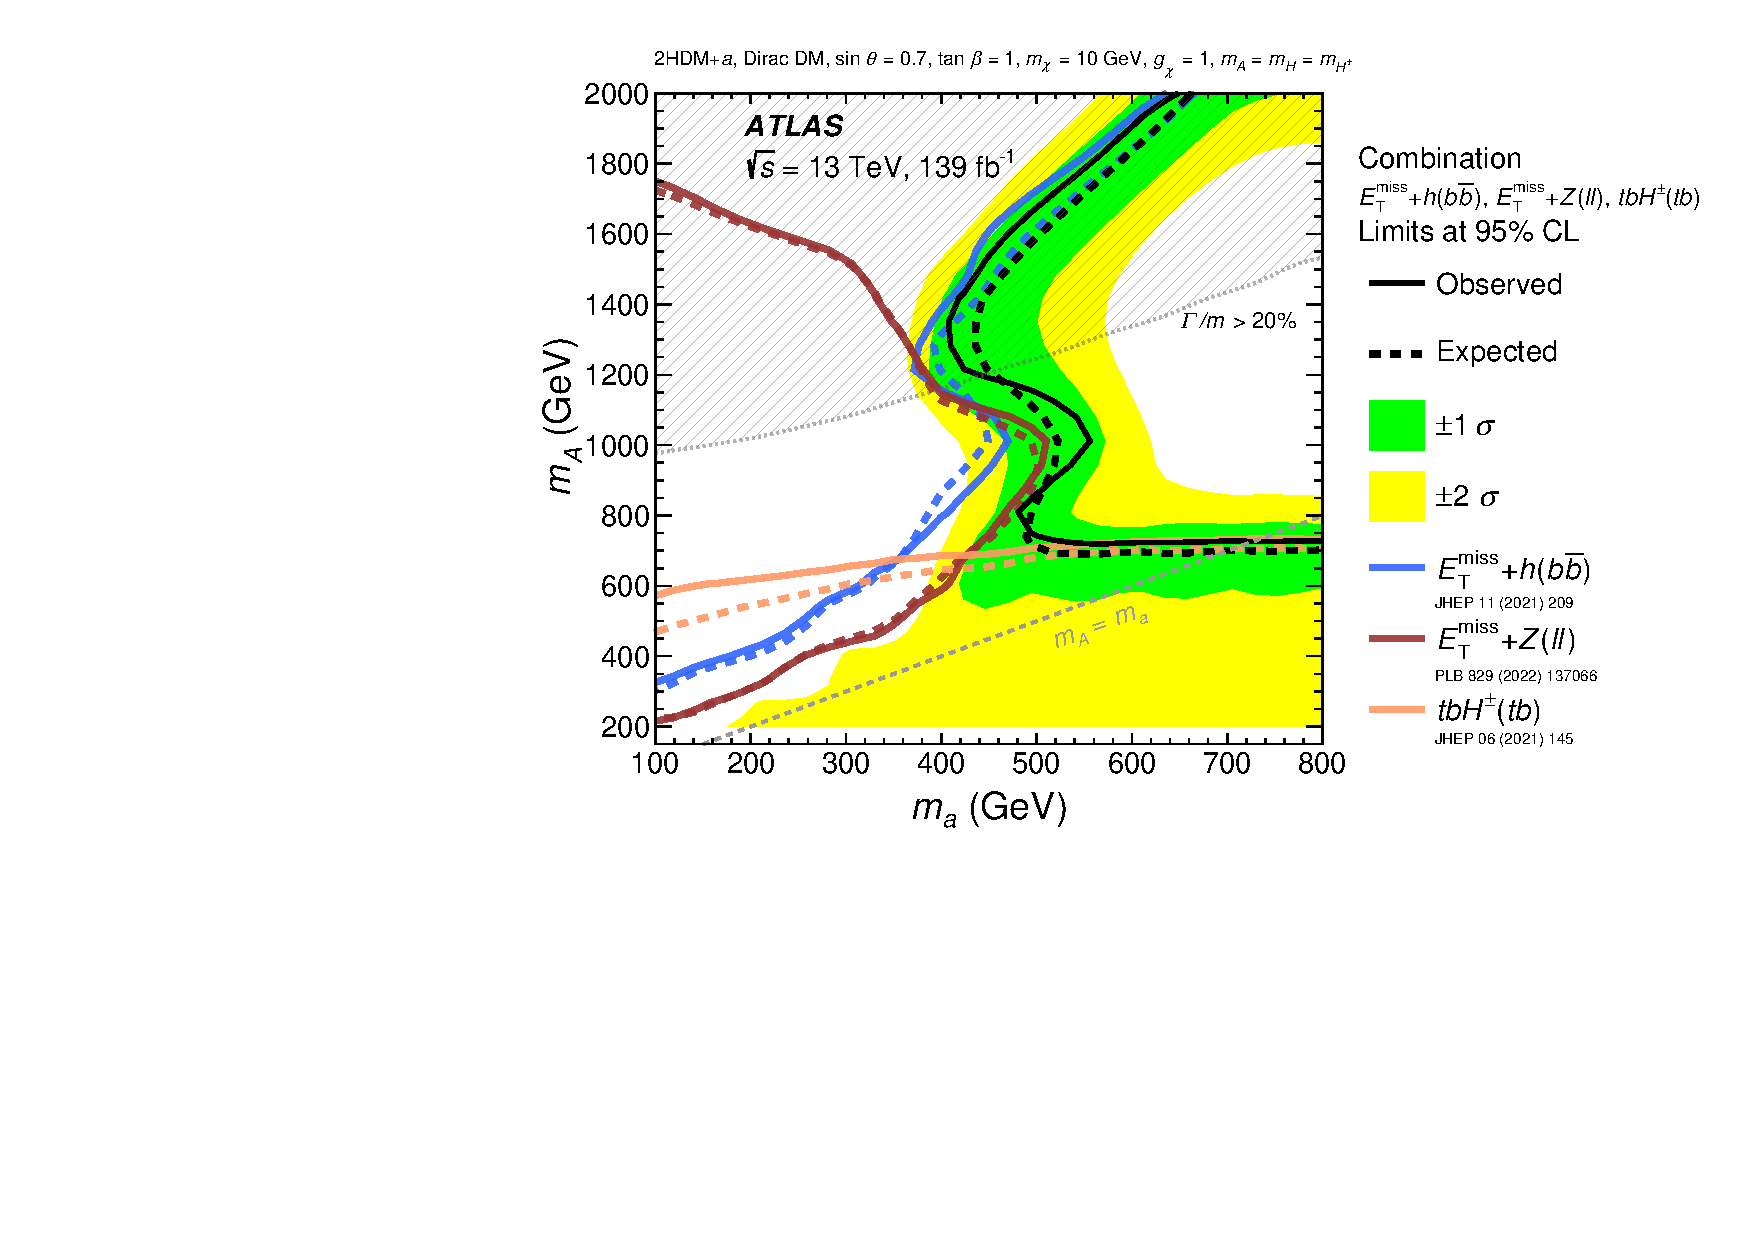
\includegraphics[width=\linewidth]{figures/fig_04b.pdf}
        \caption{}
        \label{fig:result-ma-mA-scan-b}
    \end{subfigure}
    \begin{subfigure}[2]{0.495\textwidth}
        \centering
        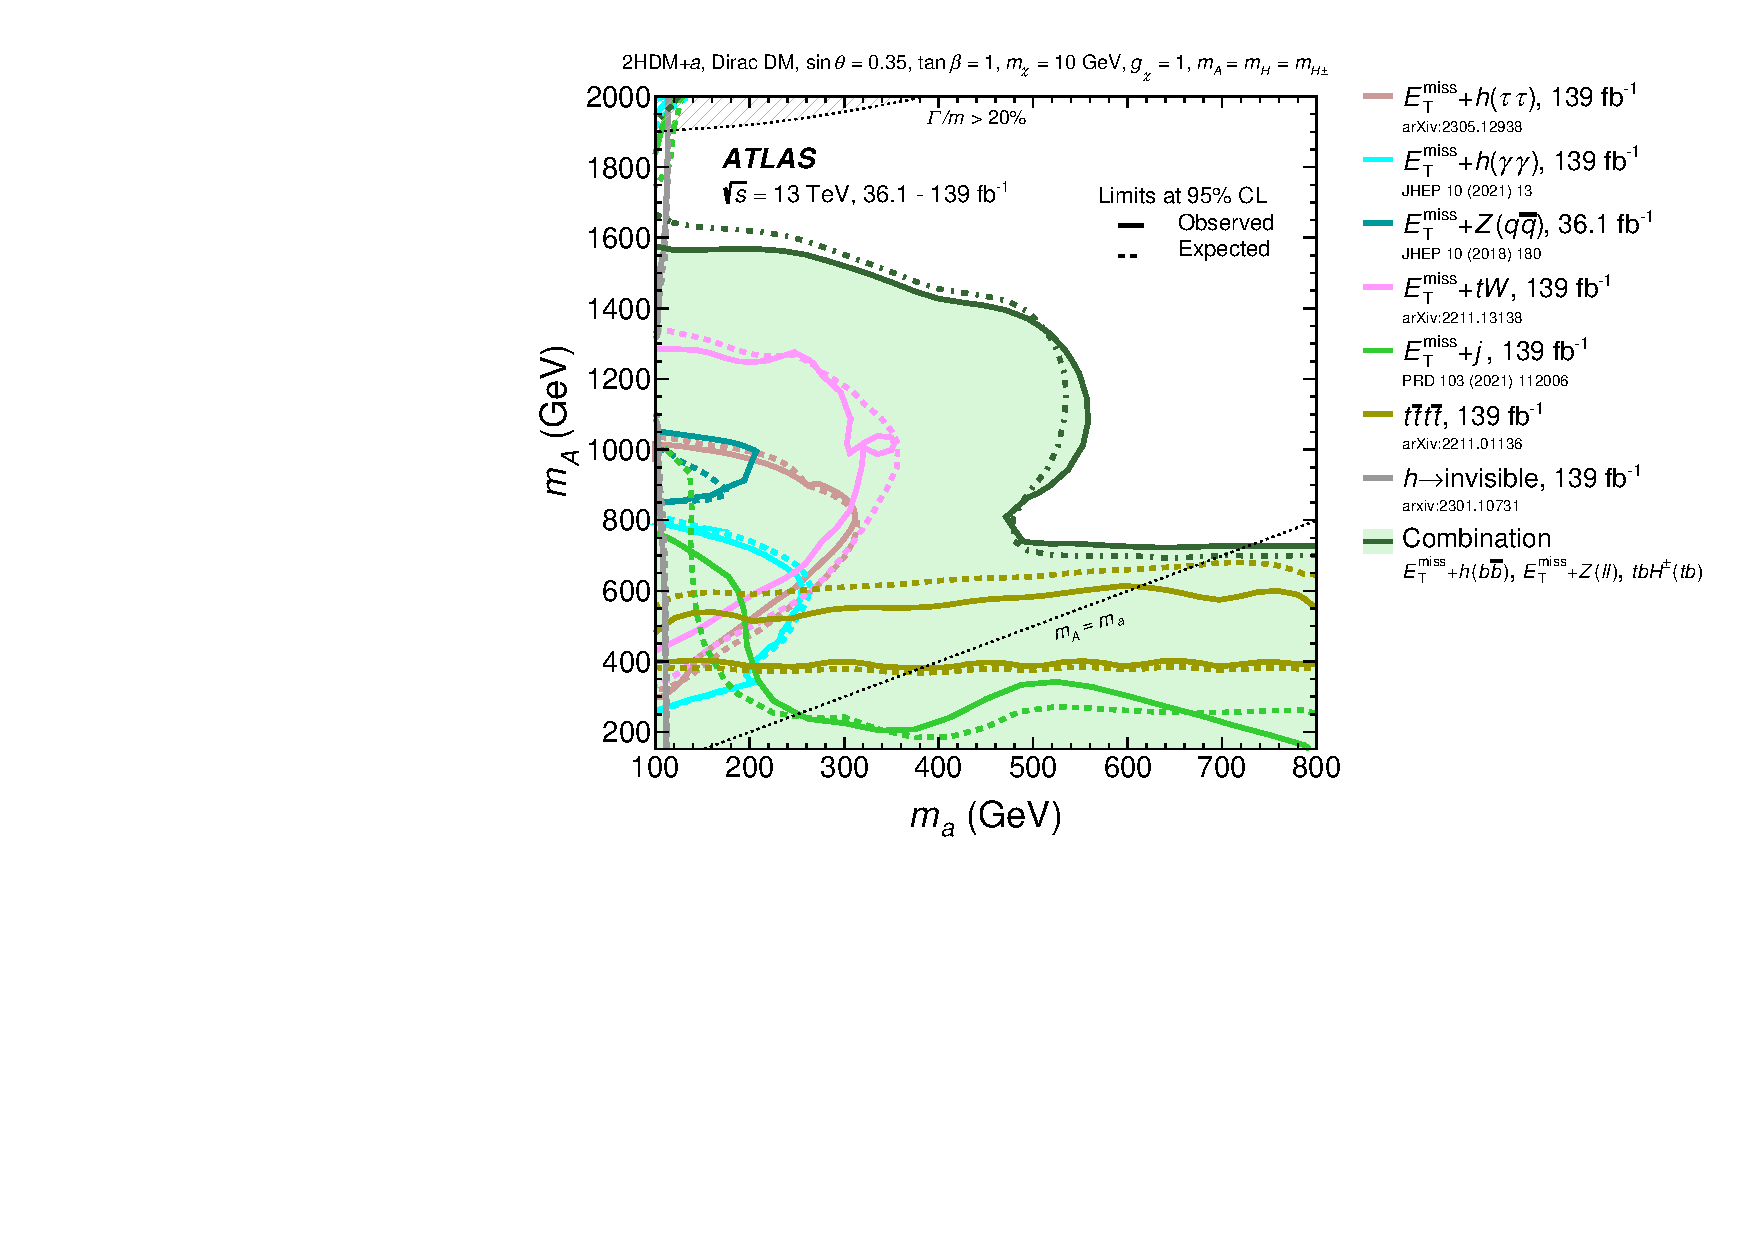
\includegraphics[width=\linewidth]{figures/fig_04c.pdf}
        \caption{}
        \label{fig:result-ma-mA-scan-c}
    \end{subfigure}
    \begin{subfigure}[2]{0.495\textwidth}
        \centering
        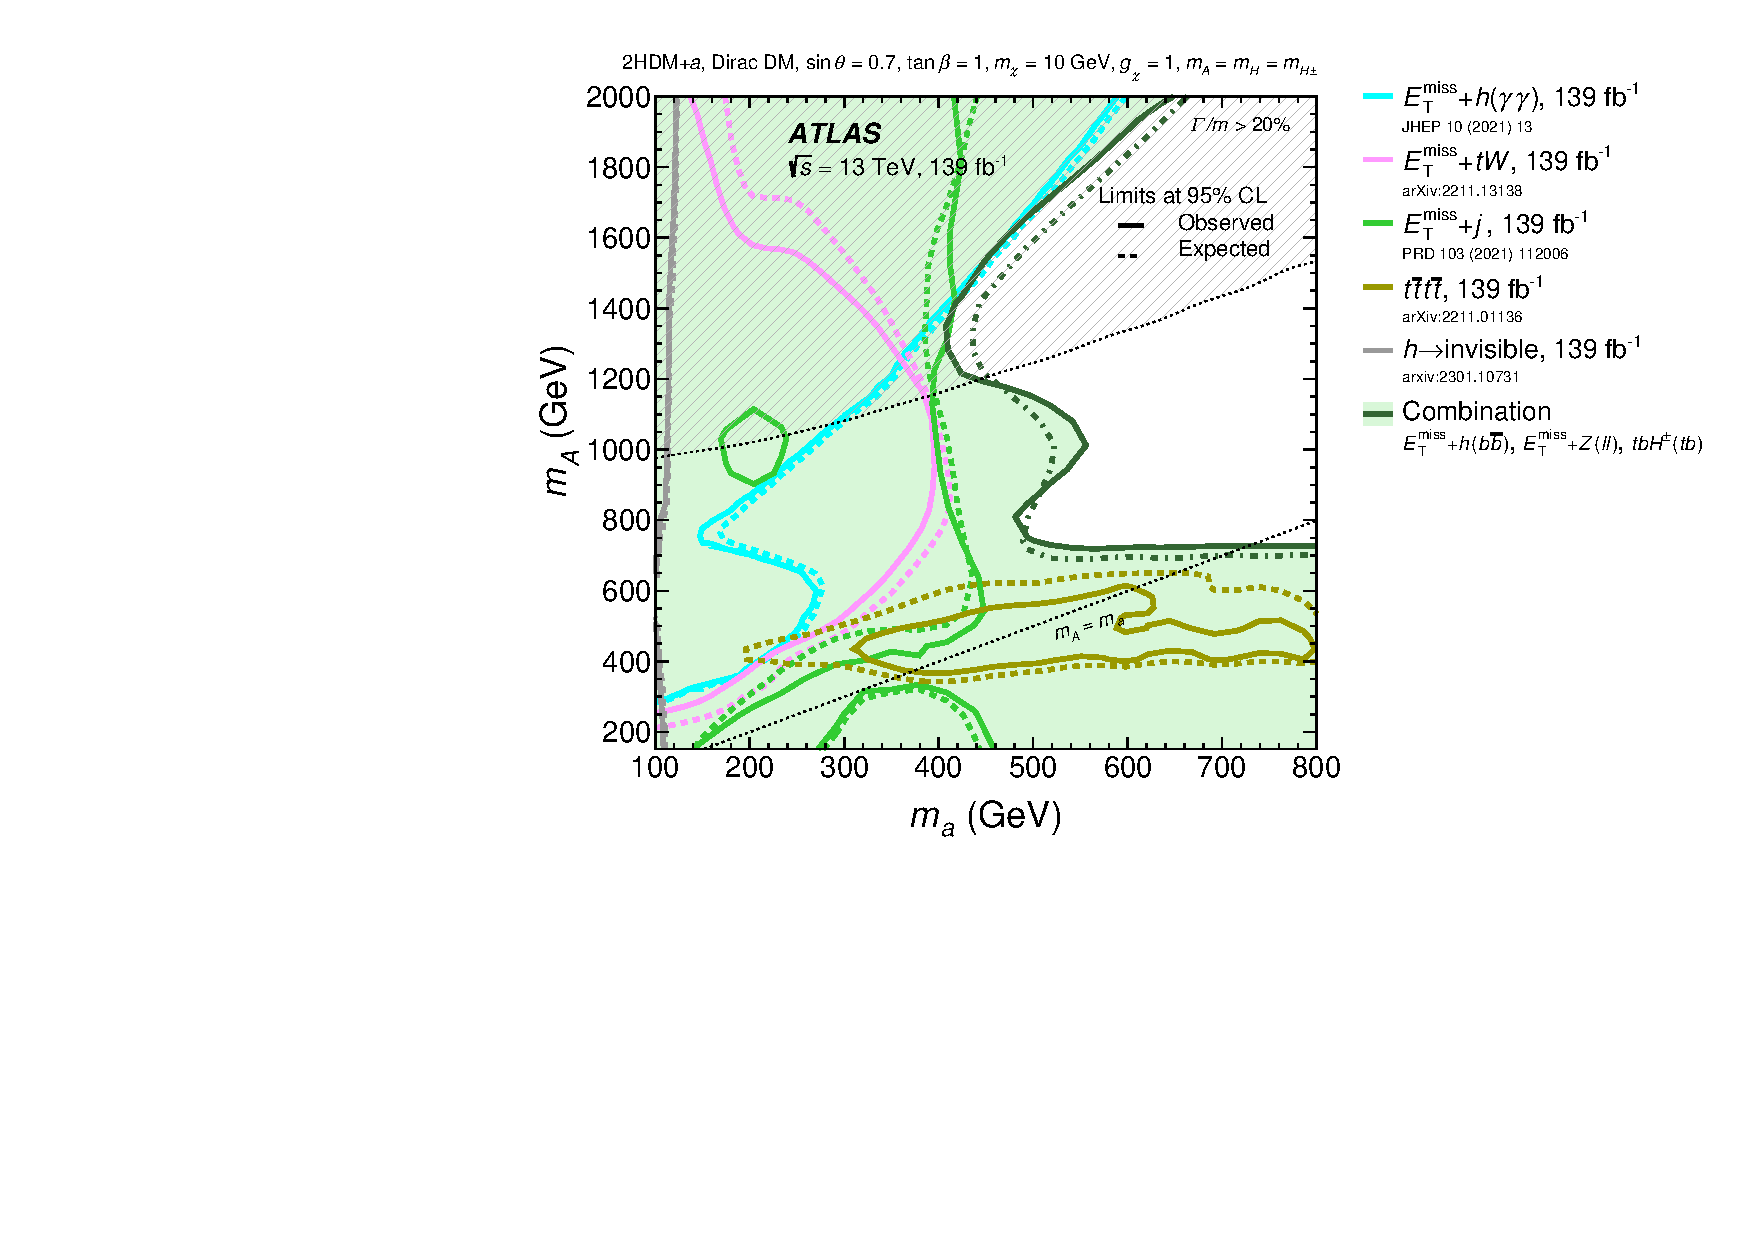
\includegraphics[width=\linewidth]{figures/fig_04d.pdf}
        \caption{}
        \label{fig:result-ma-mA-scan-d}
    \end{subfigure}
    \caption{Observed and expected exclusion regions at $95\%$ CL over the $(\ma, \mA)$ plane evaluated at \thdma mixing angles $\sint=0.35$ (subfigures (a), (c)), and $\sint=0.7$ (subfigures (b), (d)). The observed and expected contours are respectively shown in solid and dashed lines in all subsequent figures. In (a) and (b), the observed and expected exclusion limits from each of the three statistically combined signatures are shown along with the combined limits. The green and yellow shared bands respectively correspond to the $\pm1$ and $\pm2$ standard deviation uncertainty in the combined expected limits. In (c) and (d), the combined exclusion contours are overlaid along those of additional channels not included in the statistical combination. In all subfigures, a dashed grey region indicates the region where the width of any of the Higgs boson exceeds $20\%$ of its mass \cite{2hdma_comb}. }
    \label{fig:result-ma-mA-scan}
\end{figure} 

For both values of $\sint$, the $\htb$ channel excludes complementary regions where the other channels provide less exclusion power. For $\sint=0.35$ all pseudo-scalar Higgs mass up to $\mA\le 700$ GeV is excluded, and for $\sint=0.7$, the upper bound of the excluded $\mA$ ranges from 600 GeV to 700 GeV. The weak dependence on the mediator mass $\ma$ is due to the absence of the mediator in its signature, such that its sensitivity is only indirectly affected by $\ma$ via the competition from other possible decay modes, for instance $H^{\pm}\rightarrow aW^{\pm}$. The reduction in branching ratio is observed at $\sint=0.7$, where the limits from this channel weakens at lower $\ma$, where the aforementioned decay is kinematically possible. The statistical combination with $\htb$ augments the excluded parameter space above $\ma=500$ GeV and below $\mA=700$ GeV for both scenarios. 

The exclusion power of other channels not entering the statistical combination varies widely and is demonstrated on figures \ref{fig:result-ma-mA-scan-c} and \ref{fig:result-ma-mA-scan-d}. The \monohgamgam search probes a region in the parameter space that is similar in shape to that of the $\monohbb$ search, only smaller due to the smaller branching ratio of the $h\rightarrow \gamma\gamma$ decay relative to the $h\rightarrow b\bar{b}$ decay. At lower values of $\mA$ however, it becomes more sensitive than $\monohbb$, as it does not rely on the \met trigger and is capable of probing smaller values of \met, similar to the better sensitivity of $\monozll$ relative to $\monohbb$ in the same region. Similar to the $\monohbb$ search, the \monohgamgam shows a significant boost in sensitivity at higher $\mA$ for $\sint=0.7$, due to an increase in the cross-section of the $a\rightarrow ah$ process. 

The $\monohtautau$ search is only interpreted at $\sint = 0.35$, and its exclusion contour has a similar shape to that of other $\met+h$ signatures, but is even smaller in coverage due to a small branching ratio relative to the $h\rightarrow b\bar{b}$ final state. 

The exclusion contours of the $\met+tW$ search have a similar shape to those of the $\monozll$ search for both values of $\sint$, albeit smaller in exclusion area. The observed exclusion consistently covers a smaller area of the phase space than the expected sensitivity, due to a small excess in the $2$-lepton channel of less than $2\sigma$ significance \cite{EXOT-2018-43}. 

The sensitivity of the $\met+j$ search shows interesting features on the $\ma-\mA$ plane. The signature does not contain resonant production as in the case of the $Z/h$ boson in figures \ref{subfig:zll-gg-fusion-res} and \ref{subfig:hbb-gg-fusion-res}. Therefore, the exclusion contour differ significantly from the $\met+Z$ and $\met+h$ signatures. In addition, the signal cross-section is affected by the inference between non-resonant contributions from the pseudo-scalars $a$ and $A$, which depends on both $\ma$ and $\mA$, especially at the larger value of the mixing angle $\sint$ \cite{Bauer:2017ota}. A small difference in pseudo-scalar mass $(\ma\approx \mA)$ leads to destructive interference, reducing the signal cross-section and thus the sensitivity to the \hdma. This effect is observed for both values of $\sint$. At $\sint=0.35$, the $\met+j$ search excludes values of $\ma$ up to 600 GeV for $\mA\approx 200$ GeV, and values of $\mA$ up to 800 GeV for $\ma\approx 100 $ GeV. At $\sint=0.7$, stronger mixing leads to higher cross-sections for signal hypotheses with $\mA>\ma$. For $\mA\approx 1300$ GeV, all values of $\ma$ up to $\approx 400$ GeV are excluded, comparable to the exclusion power of the $\monozll$ and $\monohbb$ searches. 

The $t\bar{t}t\bar{t}$ search is sensitive in regions where the $\monozll$ and $\monohbb$ searches have lower sensitivity, similar to the $\htb$ search. However, unlike the latter, it is only sensitive to the \thdma when either of the pseudo-scalar masses is above the production threshold of a top quark pair $(m_{A/a}\ge 2m_t)$. For $\sint = 0.35$, the contour is almost independent of $\ma$, driven largely by the resonant production of the heavy Higgs bosons $A/H$. For $\sint = 0.7$, the sensitivity is lowered for small $\ma$ compared to the scenario with $\sint=0.35$ due to a larger $a/A$ and a forbidden $a\rightarrow t\bar{t}$ decay.

The exclusion contours from the $\met + Z(q\bar{q})$ search on 36 $\ifb$ data are shown for scenario 1a \cite{EXOT-2017-32}. The search provides the smallest sensitivity because it suffers from larger multijet production backgrounds and smaller data sample.

\subsection{Scenario 2: \texorpdfstring{$\mA-\tanb$}{TEXT} planes}

Figure \ref{fig:result-mA-tanb-scan} summarizes the exclusion limits over the $\mA-\tanb$ parameter plane evaluated with $\sint = 0.35$ and $\sint = 0.7$. In both scenarios, a large portion of the parameter plane is excluded by the combined contours. At $\sint=0.35$ the combined sensitivity is driven primarily by the $\monozll$ search, which is also observed at lower pseudo-scalar mass at $\sint=0.7$. At higher values of $\mA$, the $\monohbb$ provides stronger constraints. In general, the sensitivity of these channels is influence by the transition from $gg$- to $bb$-initiated production of the $Z/h$ boson, and finds its minimum in the region around $\tanb=5$. 

\begin{figure}[h!]
    \centering
    \begin{subfigure}[2]{0.495\textwidth}
        \centering
        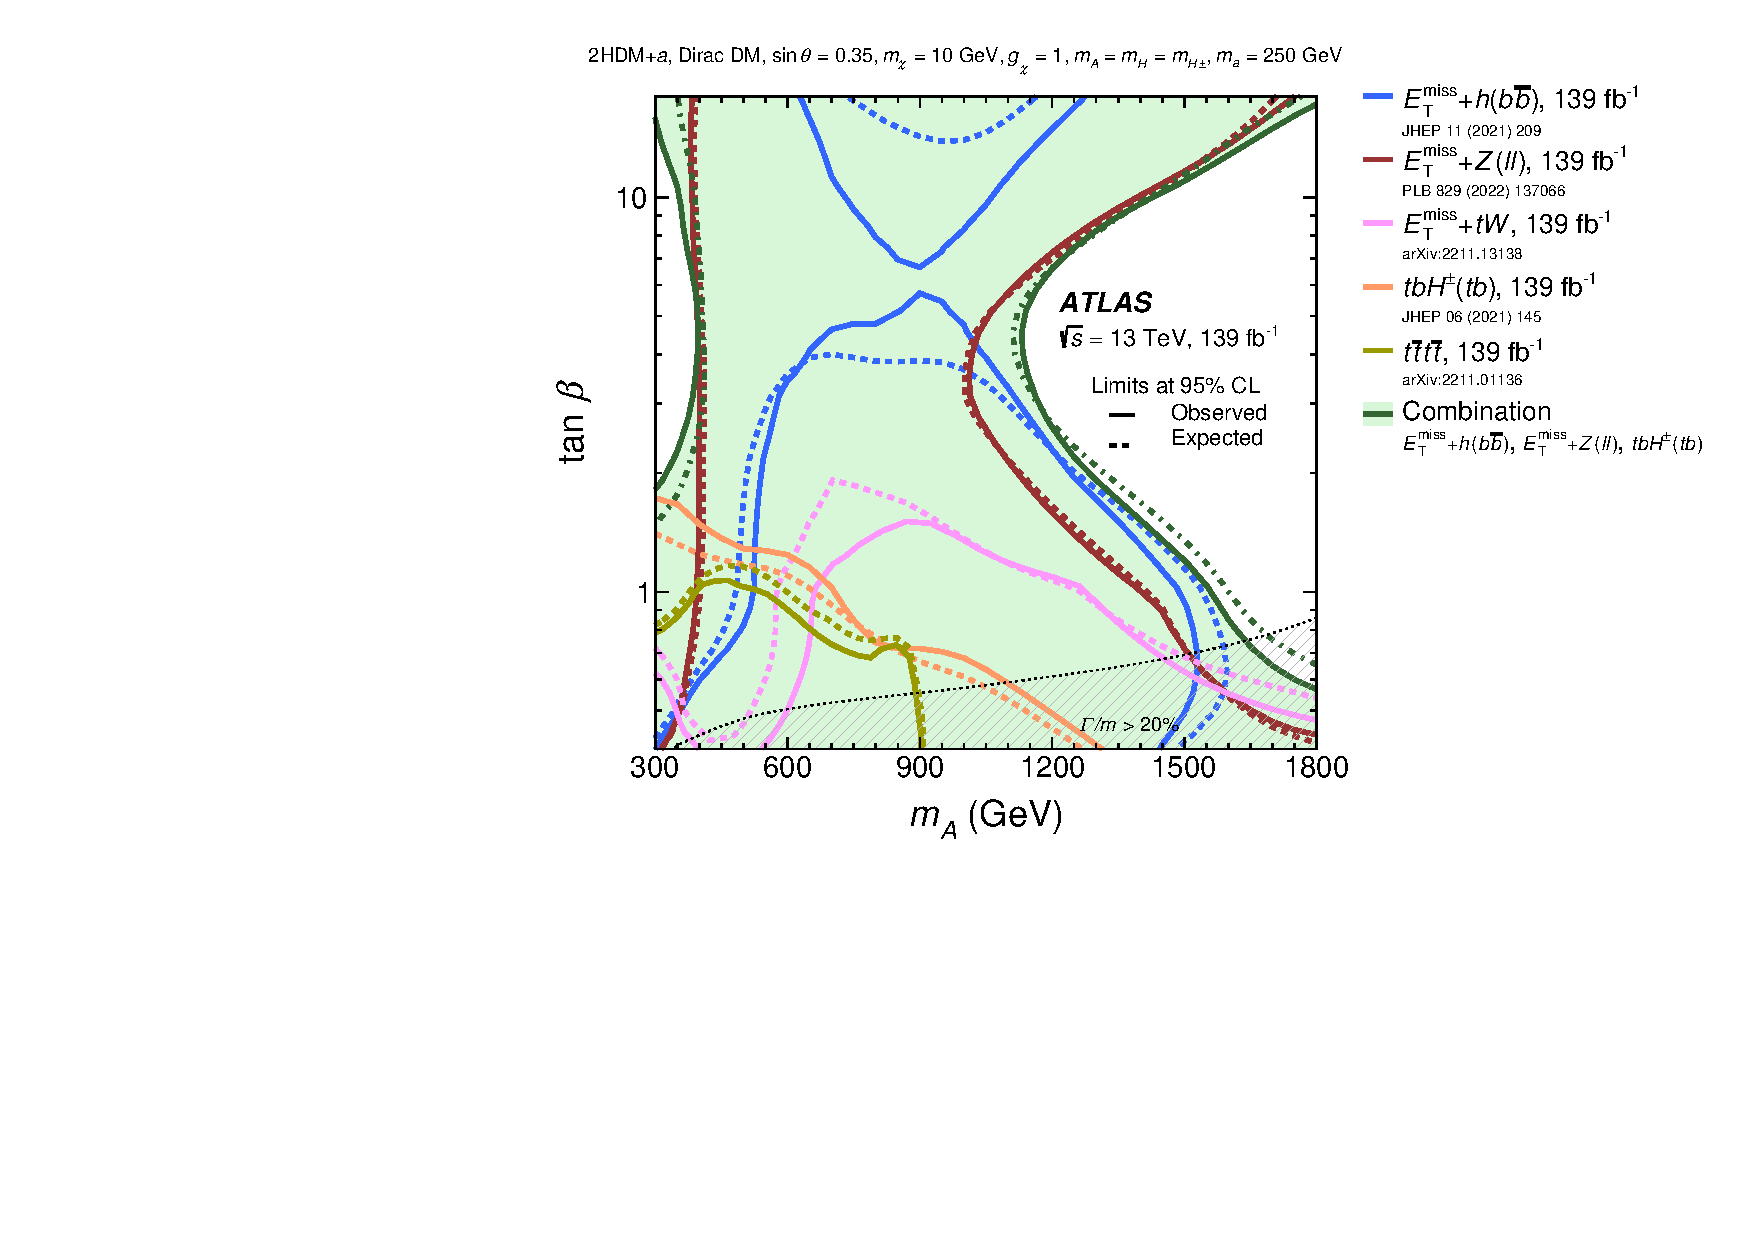
\includegraphics[width=\linewidth]{figures/fig_05a.pdf}
        \caption{}
        \label{fig:result-mA-tanb-scan-a}
    \end{subfigure}
    \begin{subfigure}[2]{0.495\textwidth}
        \centering
        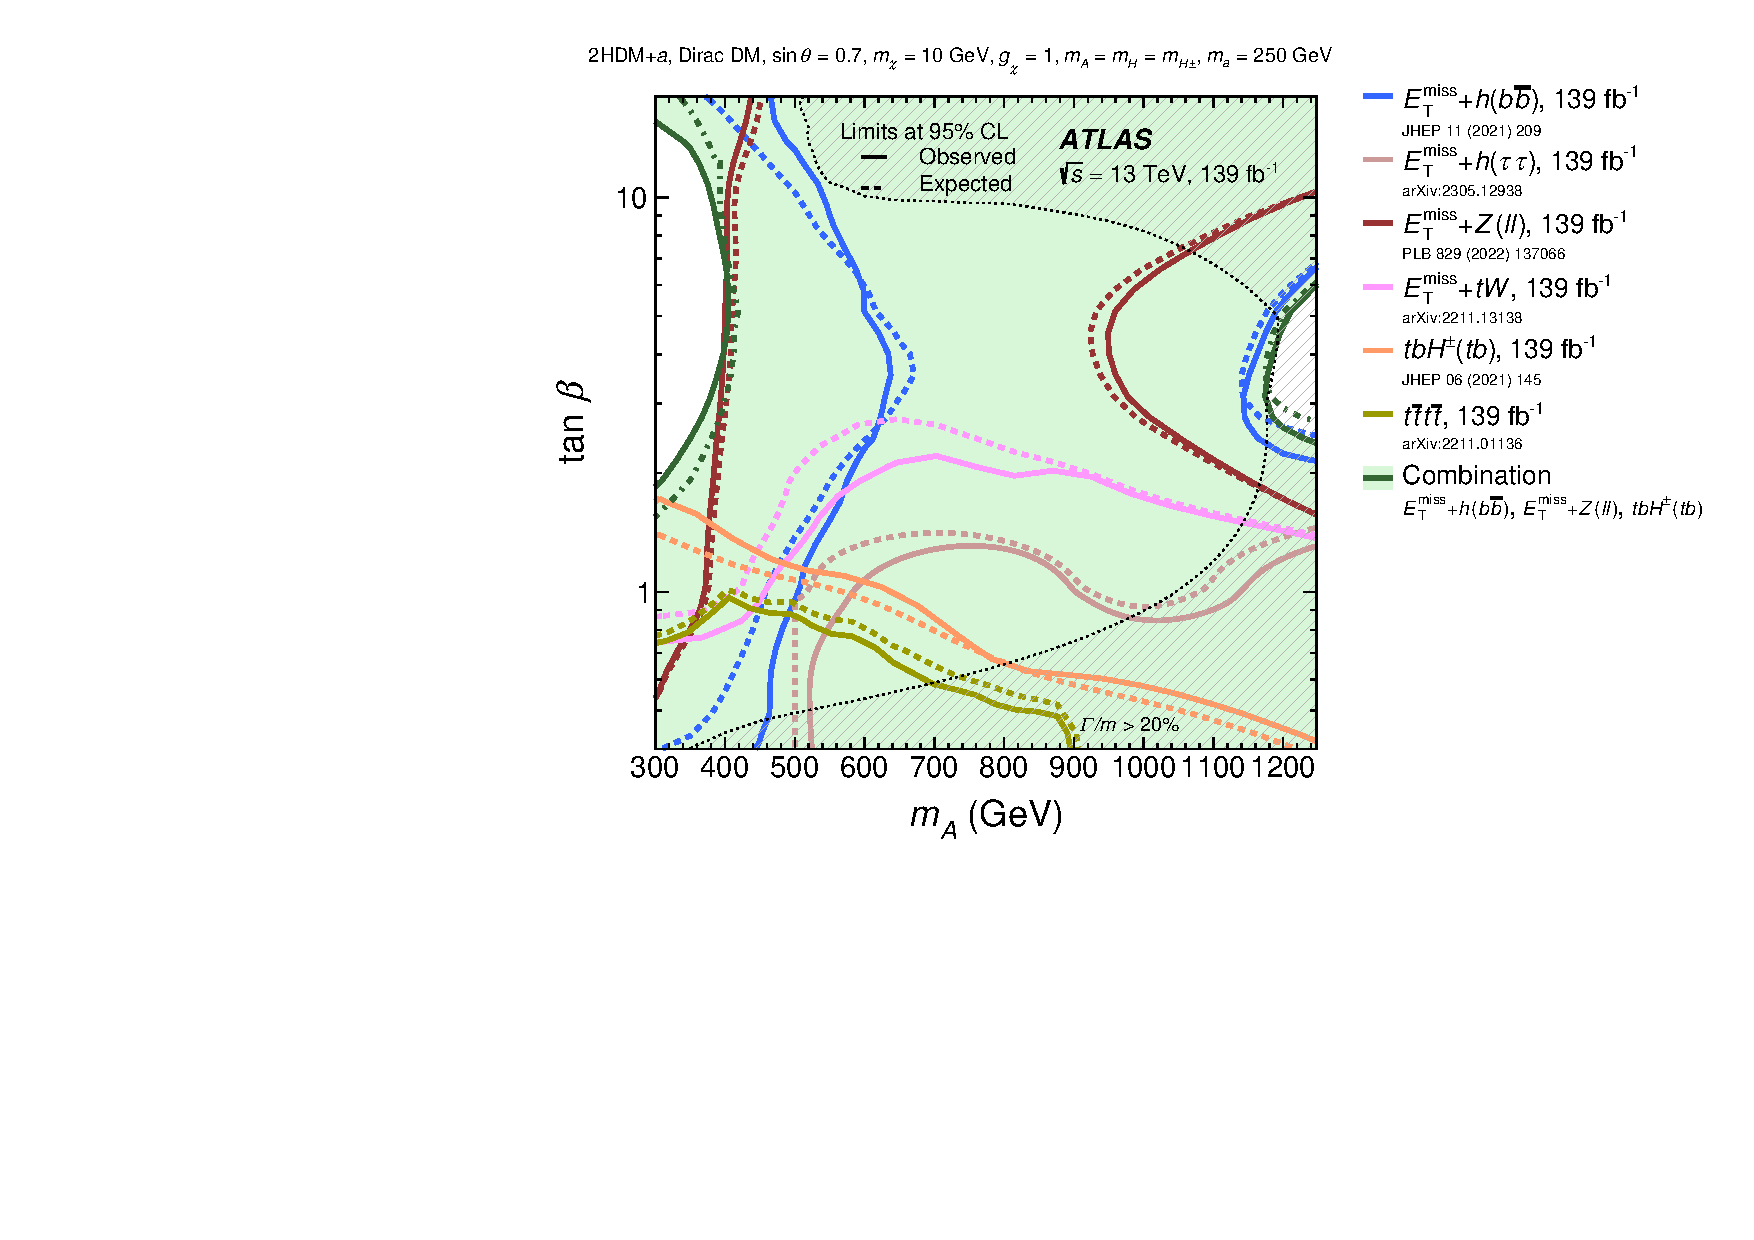
\includegraphics[width=\linewidth]{figures/fig_05b.pdf}
        \caption{}
        \label{fig:result-mA-tanb-scan-b}
    \end{subfigure}
    \caption{Observed and expected exclusion regions at $95\%$ CL over the $(\mA, \tanb)$ plane evaluated at \thdma mixing angles $\sint=0.35$ (a), and $\sint=0.7$ (b). The statistical combined contours are shown along with those from individual searches. In both subfigures, a dashed grey region indicates the region where the width of any of the Higgs boson exceeds $20\%$ of its mass \cite{2hdma_comb}. }
    \label{fig:result-mA-tanb-scan}
\end{figure} 

The $\met+tW$ search excludes regions of the parameter space up to $\tanb=1.5$ for $\sint=0.35$ and $\tanb=2$ for $\sint=0.7$. The observed sensitivity in both scenarios is weaker than the expected counterpart because of a small excess in the two-lepton signal region of the search \cite{EXOT-2018-43}. The larger mixing angle again shows better sensitivity to the $\met+tW$ signature \cite{Pani:2017qyd}. 

The exclusion contour from the $\met+h(\tau\tau)$ search is evaluated as a function of $\mA$ and $\tanb$ only at $\sint=0.7$. Because of the small branching ratio of the $h\rightarrow \tau\tau$ decay, it has low sensitivity for the \thdma signal. 

The $t\bar{t}t\bar{t}$ and $\htb$ searches provide sensitivity at low values of $\mA$ and $\tanb$, due to enhanced production cross-section for smaller resonance masses and a preference for coupling to third generation quarks in this region.

\subsection{Scenario 3: \texorpdfstring{$\ma-\tanb$}{TEXT} planes}

Figure \ref{fig:result-ma-tanb-scan} summarizes the exclusion limits as a function of the $\ma$ and $\tanb$ evaluated at $\sint = 0.35$ (scenario 3a) and $\sint = 0.7$ (scenario 3b). In both scenarios, the $\monozll$ search drives the sensitivity over a large portion of the parameter plane. The $\monohbb$ and \monohgamgam searches exclude analogous regions, albeit the latter covers a smaller area, due to the smaller $h\rightarrow \gamma\gamma$ branching ratio. Both channels observe decreased sensitivity at $\tanb\approx 5$ as the $gg$-initiated production transitions to the $bb$-initiated counterpart. 

\begin{figure}[h!]
    \centering
    \begin{subfigure}[2]{0.495\textwidth}
        \centering
        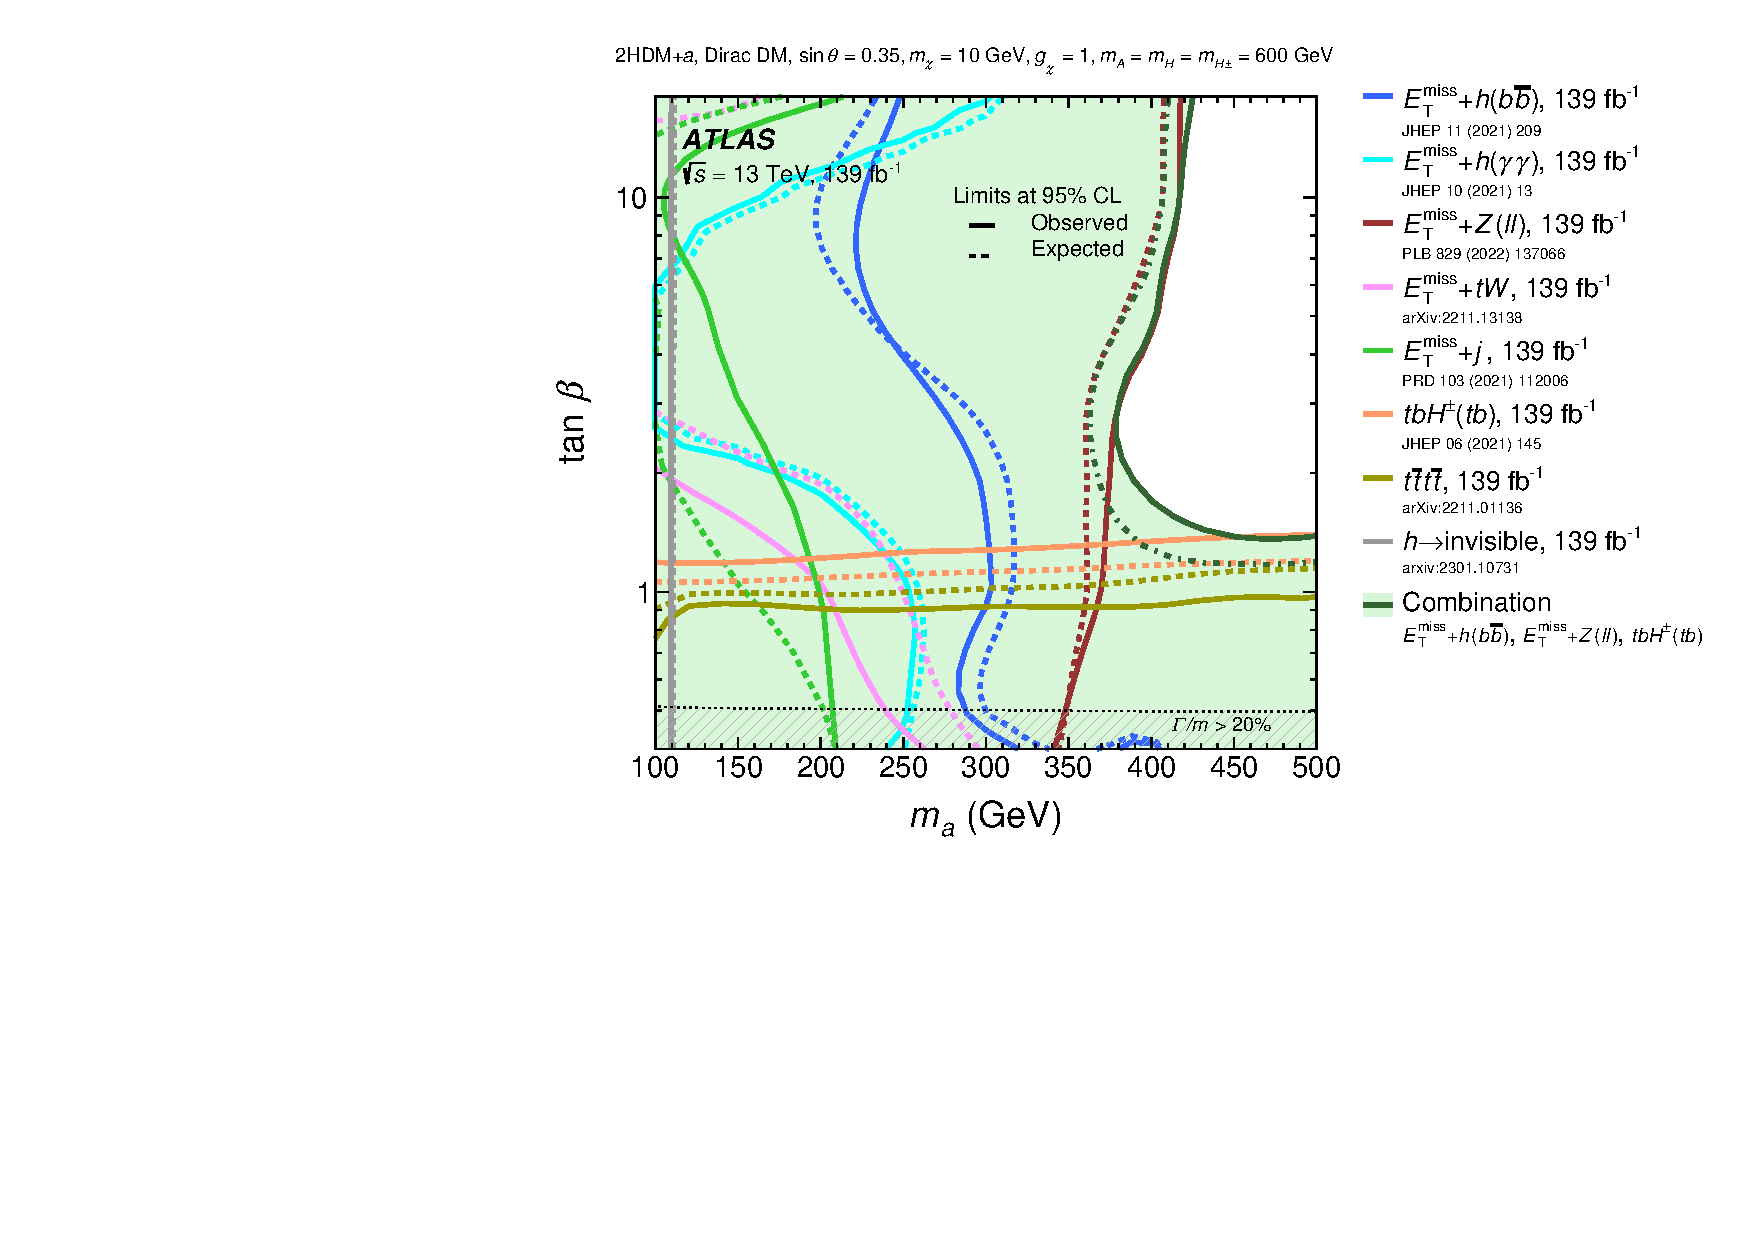
\includegraphics[width=\linewidth]{figures/fig_06a.pdf}
        \caption{}
        \label{fig:result-ma-tanb-scan-a}
    \end{subfigure}
    \begin{subfigure}[2]{0.495\textwidth}
        \centering
        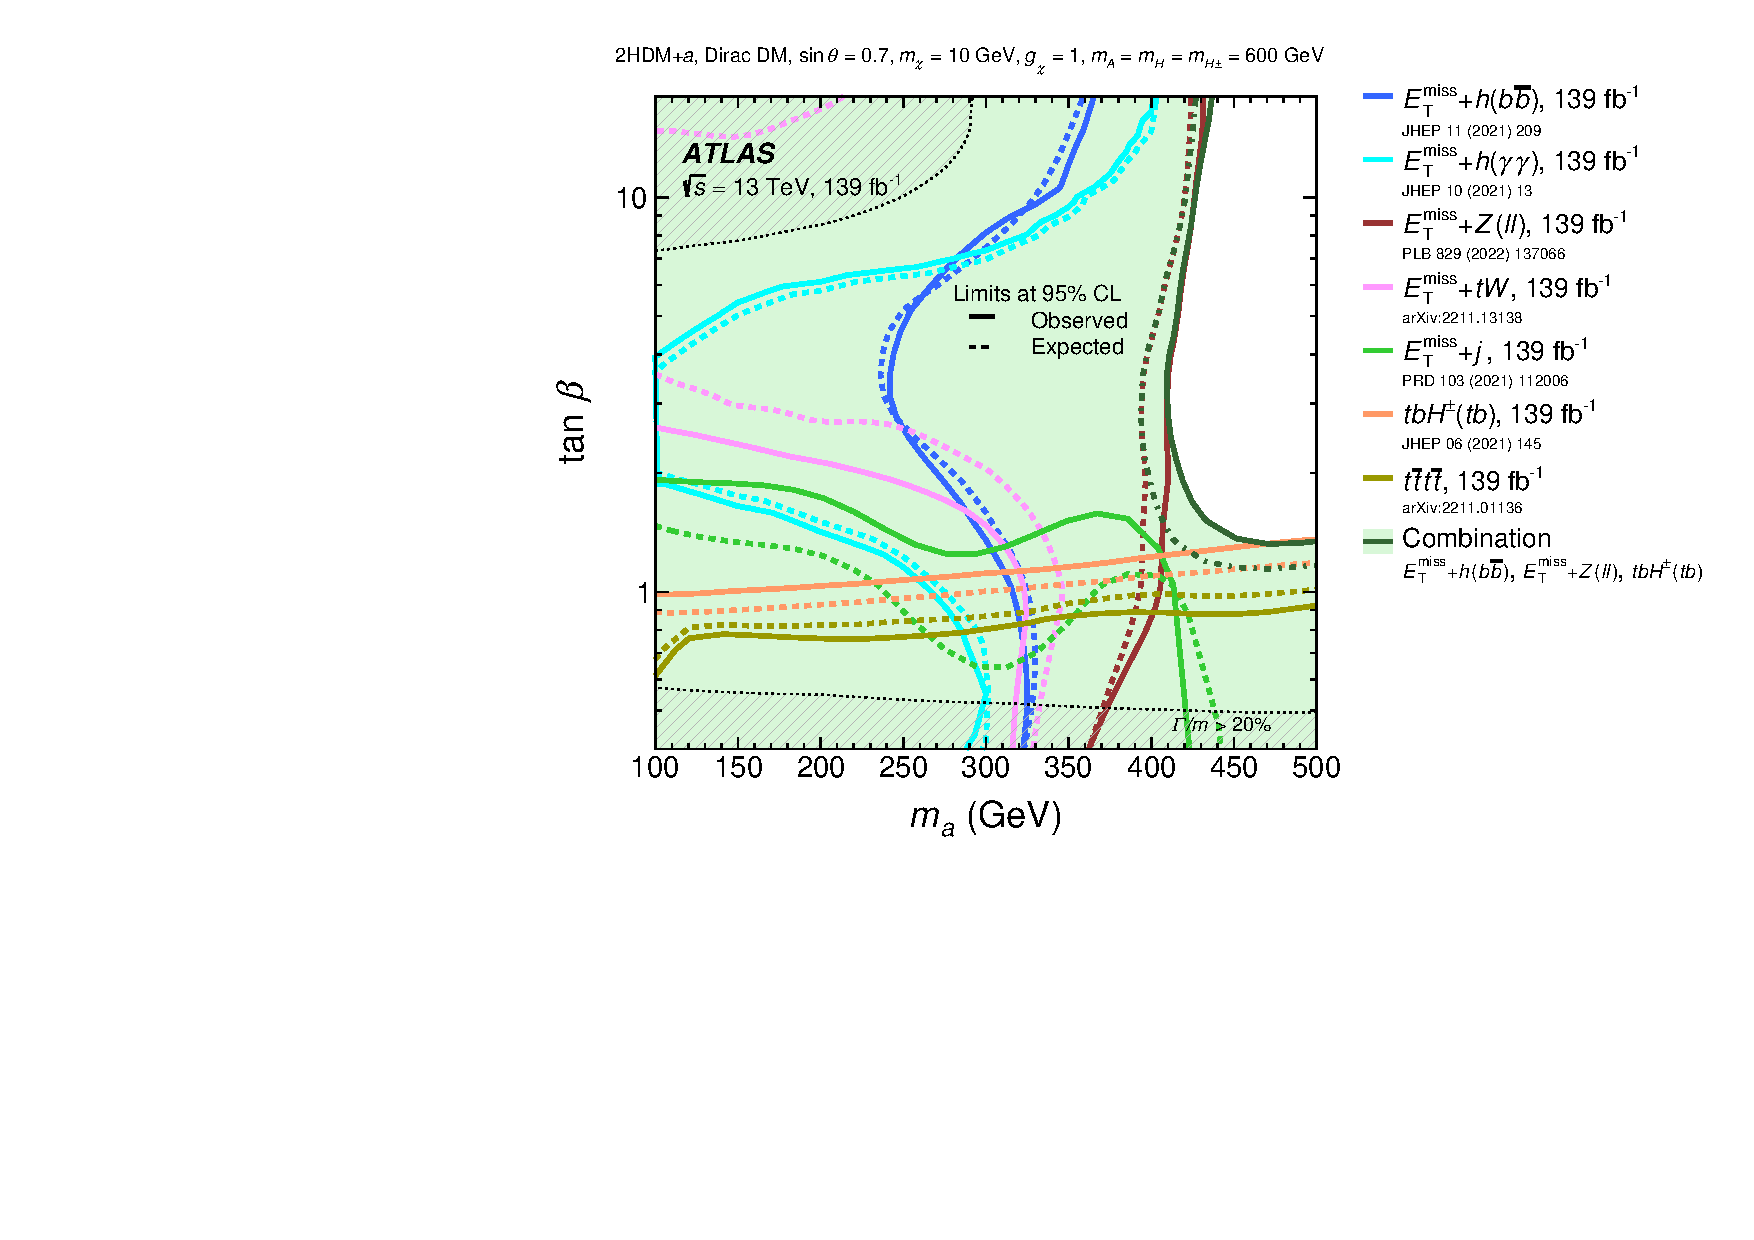
\includegraphics[width=\linewidth]{figures/fig_06b.pdf}
        \caption{}
        \label{fig:result-ma-tanb-scan-b}
    \end{subfigure}
    \caption{Observed and expected exclusion regions at $95\%$ CL over the $(\ma, \tanb)$ plane evaluated at \thdma mixing angles $\sint=0.35$ (a), and $\sint=0.7$ (b). The statistical combined contours are shown along with those from individual searches. In both subfigures, a dashed grey region indicates the region where the width of any of the Higgs boson exceeds $20\%$ of its mass \cite{2hdma_comb}. }
    \label{fig:result-ma-tanb-scan}
\end{figure} 

The $\met+tW$ search excludes regions of the parameter space at low $\tanb$ and low $\ma$. Better sensitivity is observed for the larger $A/a$ mixing angle. 

The $\met+j$ search excludes signal hypotheses characterized by low values of $\ma$ and $\tanb$, and its sensitivity is enhanced at $\sint=0.7$ due to more significant $a/A$ mixing, enlarging the signal cross-sections for $\mA>\ma$. 

The $\hinv$ decay suffers from small branching ratio and thus provides sensitivity at low values of $\ma$, independent of $\tanb$.

The $t\bar{t}t\bar{t}$ and $\htb$ searches constrain regions complementary to the $\met+X$ signatures. It is sensitive at low $\tanb$ and almost independent of $\ma$.

\subsection{Scenario 4: Variation of \texorpdfstring{$\sint$}{TEXT}}

Figure \ref{fig:result-sint-scan} summarizes the exclusion limits as a function of $\sint$ for the \thdma under both low- and high-mass mediator hypotheses. The upper row shows the results for the baseline parameter choice of Scenario 4, in which $\tanb=1.0$, and the lower row additional results obtained for alternative values of $\tanb$, namely $\tanb=0.5$ and $\tanb=50$. Exclusion limits shown in the subfigures on the left are derived at $\mA=600$ GeV, $\ma=200$ GeV, corresponding to scenario 4a and the low-mass hypothesis, and those on the right at $\mA=1.0$ TeV, $\ma=350$ GeV, corresponding to scenario 4b and the high-mass hypothesis. The exclusion limits are represented by the ratio of the excluded cross-section to the nominal cross-section of the signal model.

\begin{figure}[h!]
    \centering
    \begin{subfigure}[2]{0.495\textwidth}
        \centering
        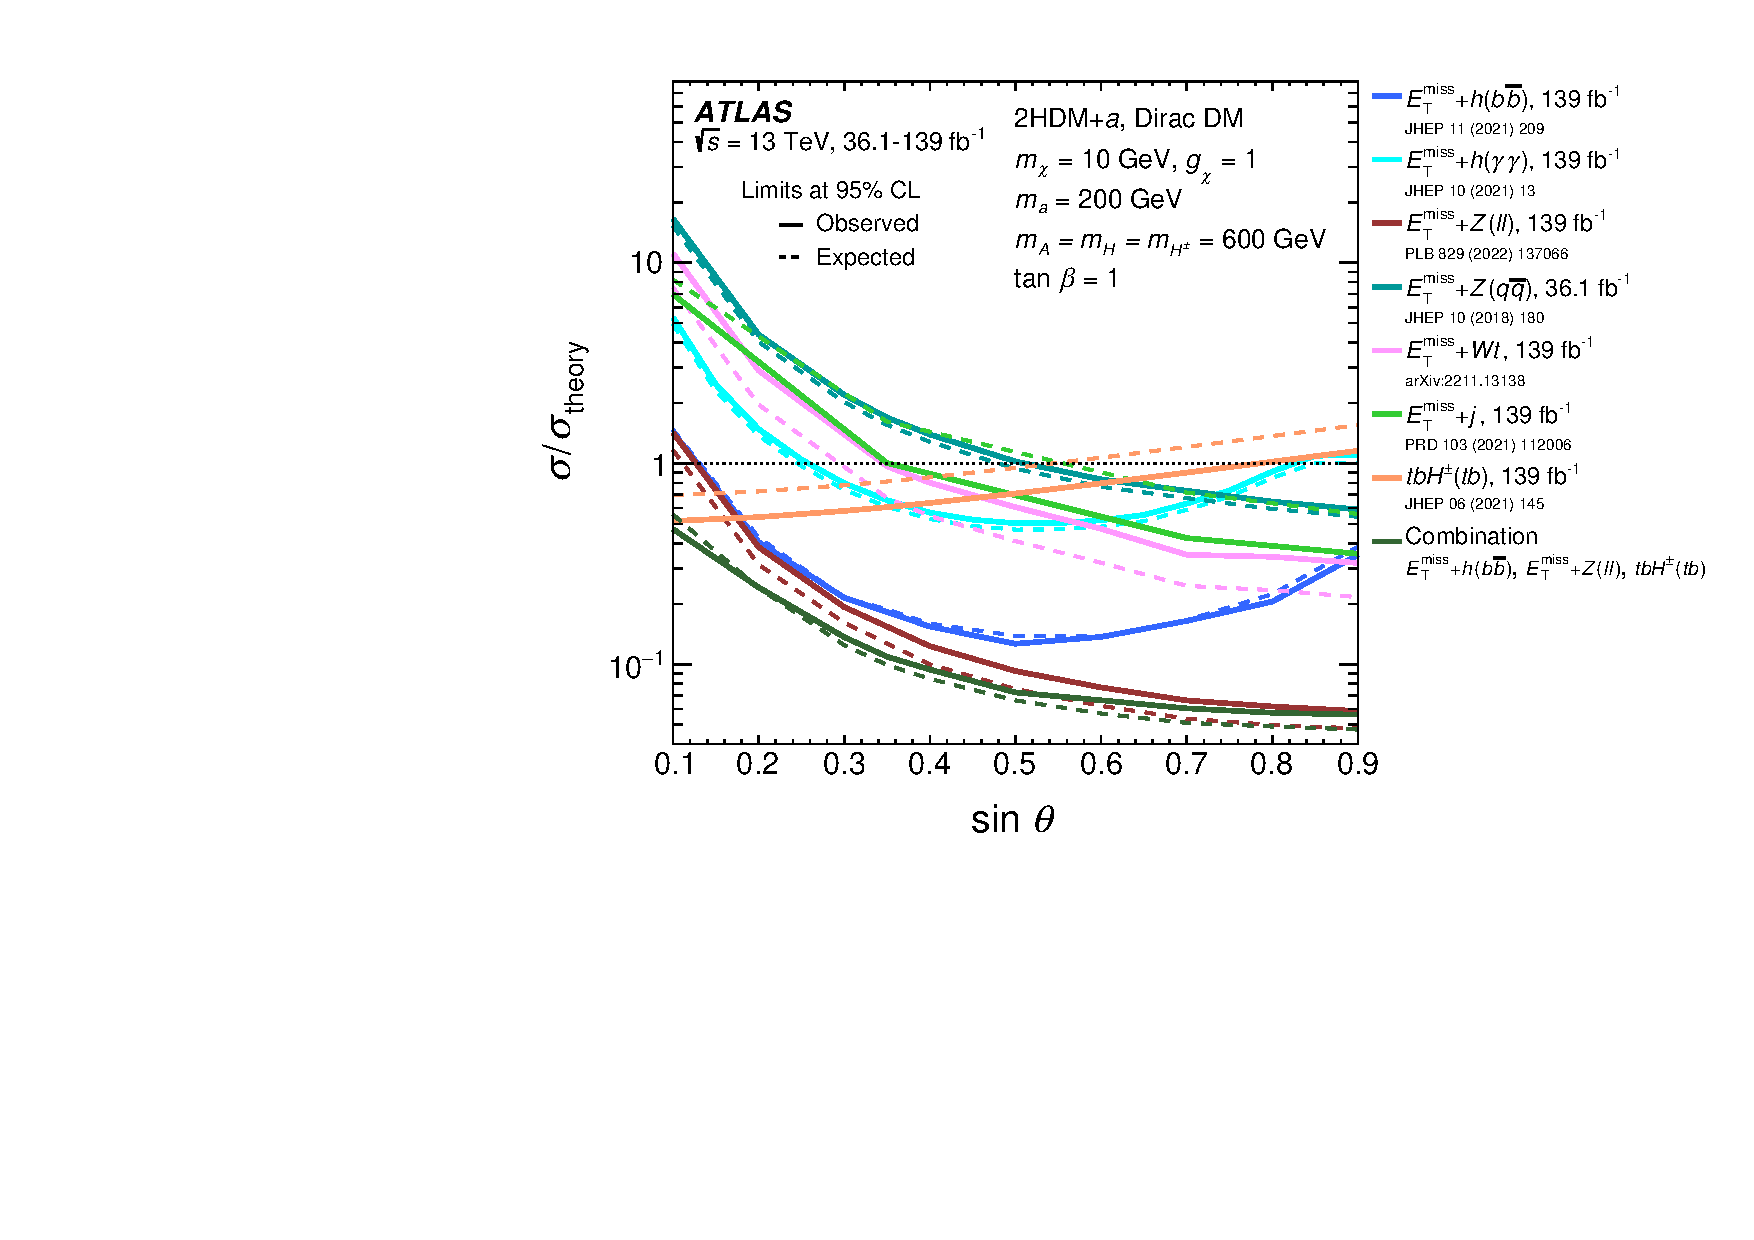
\includegraphics[width=\linewidth]{figures/fig_07a.pdf}
        \caption{}
        \label{fig:result-sint-scan-a}
    \end{subfigure}
    \begin{subfigure}[2]{0.495\textwidth}
        \centering
        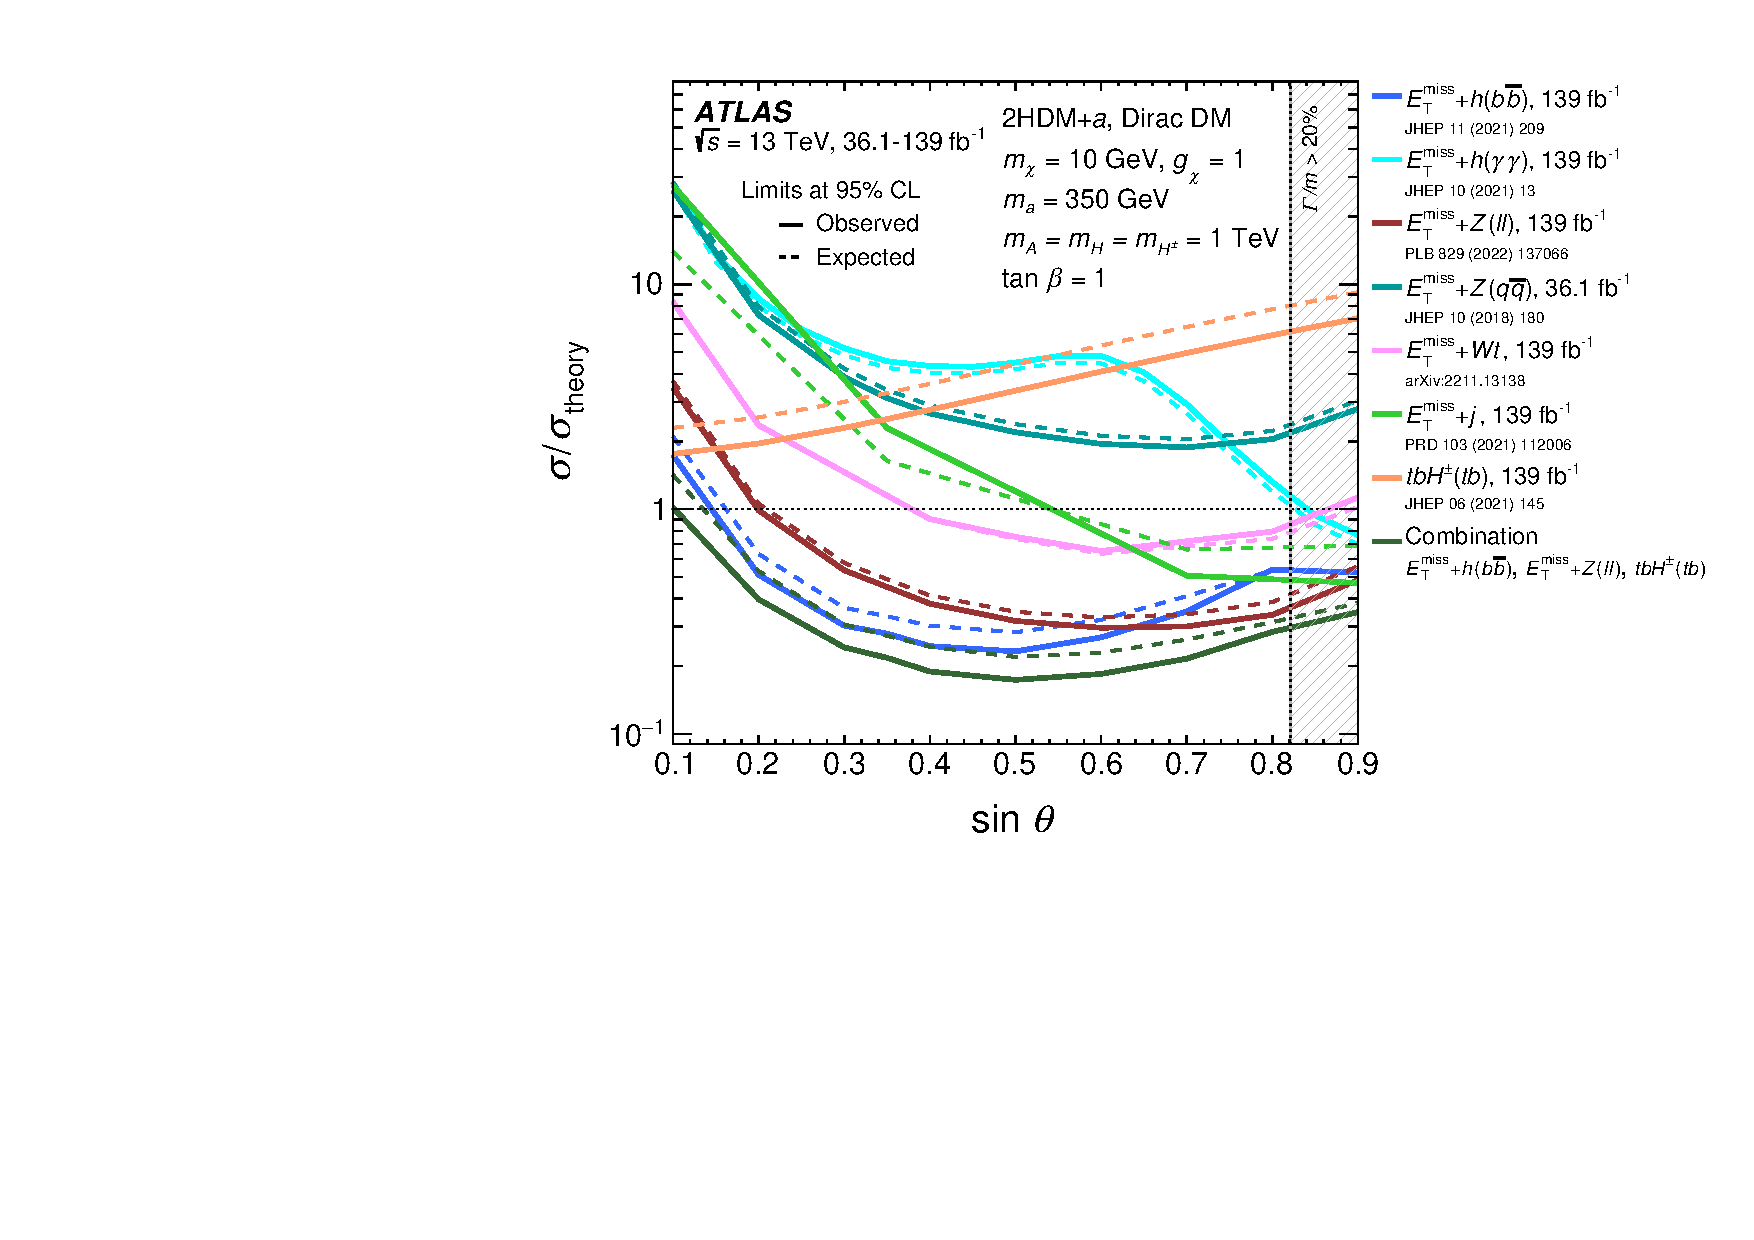
\includegraphics[width=\linewidth]{figures/fig_07b.pdf}
        \caption{}
        \label{fig:result-sint-scan-b}
    \end{subfigure}
    \begin{subfigure}[2]{0.495\textwidth}
        \centering
        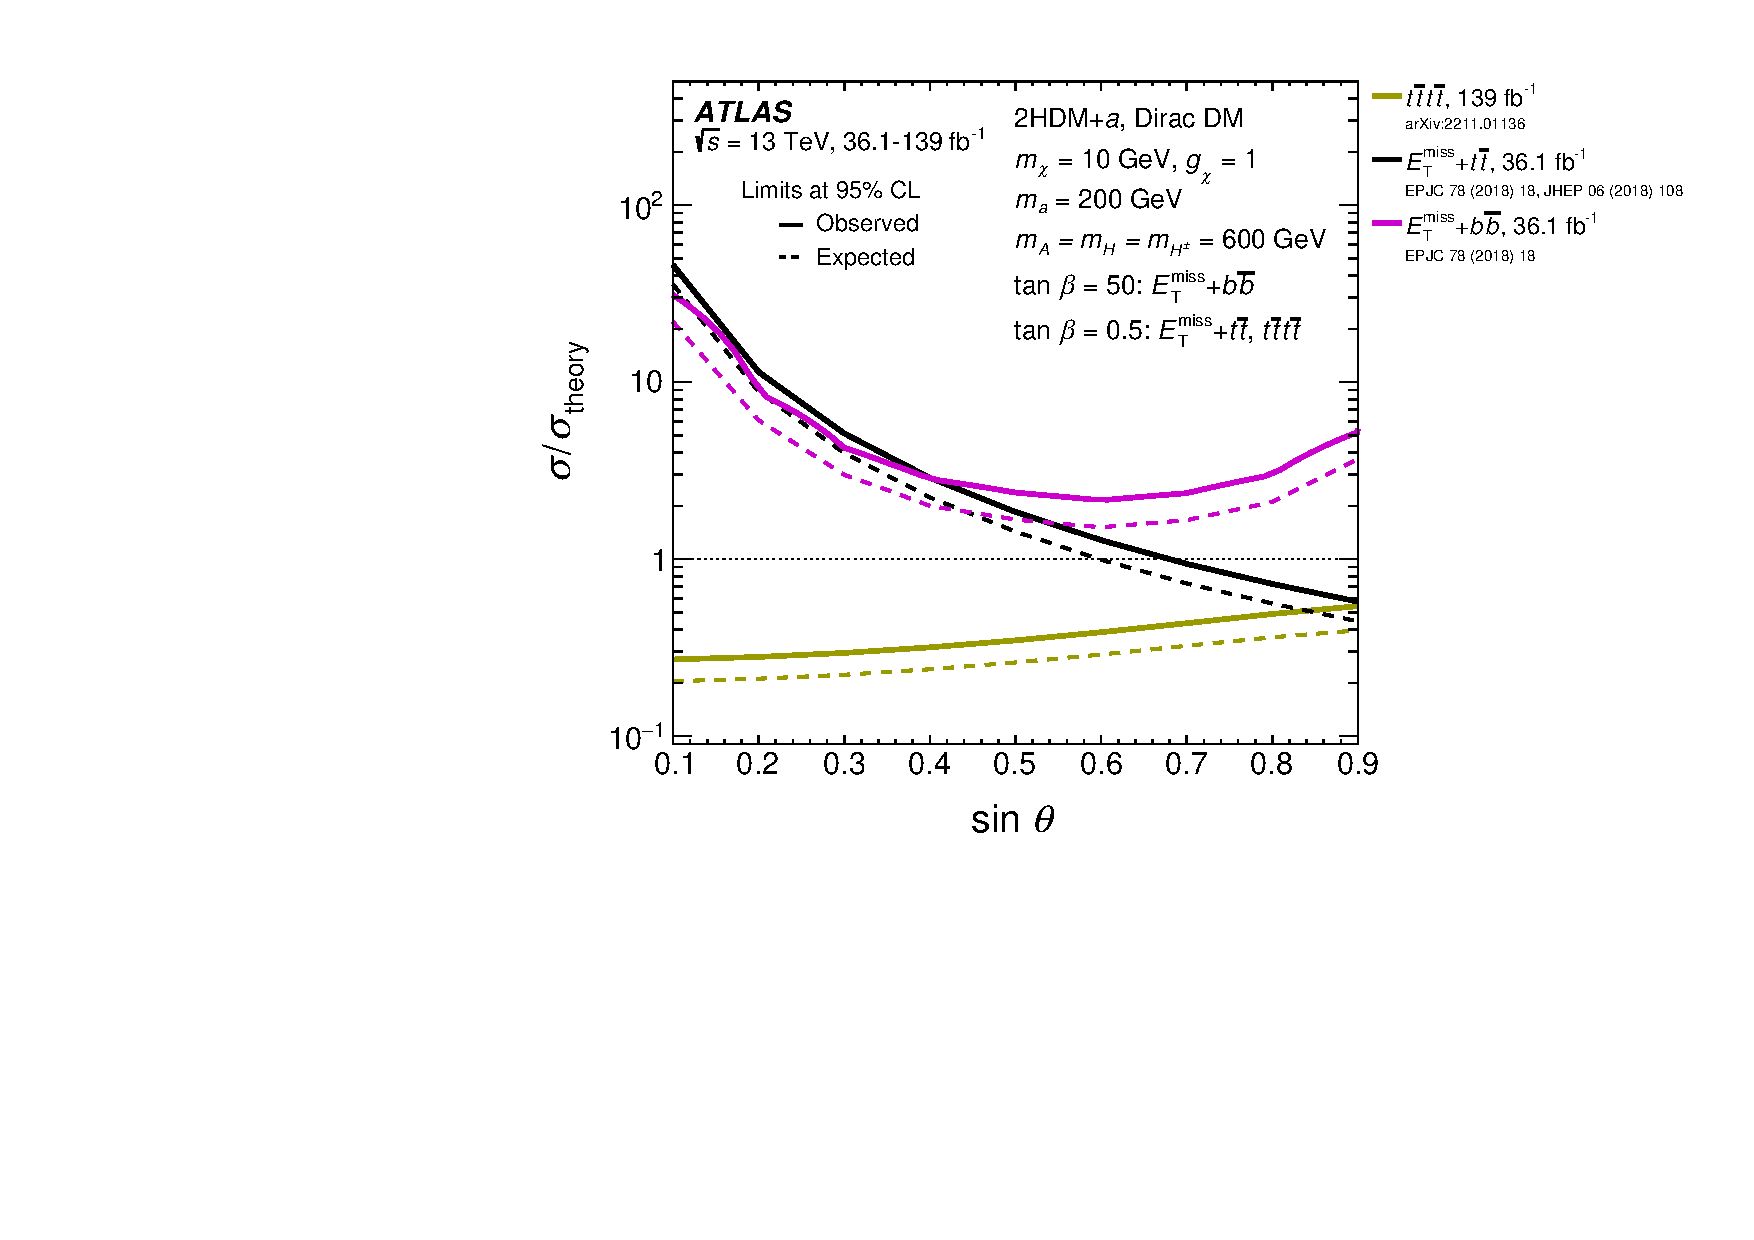
\includegraphics[width=\linewidth]{figures/fig_07c.pdf}
        \caption{}
        \label{fig:result-sint-scan-c}
    \end{subfigure}
    \begin{subfigure}[2]{0.495\textwidth}
        \centering
        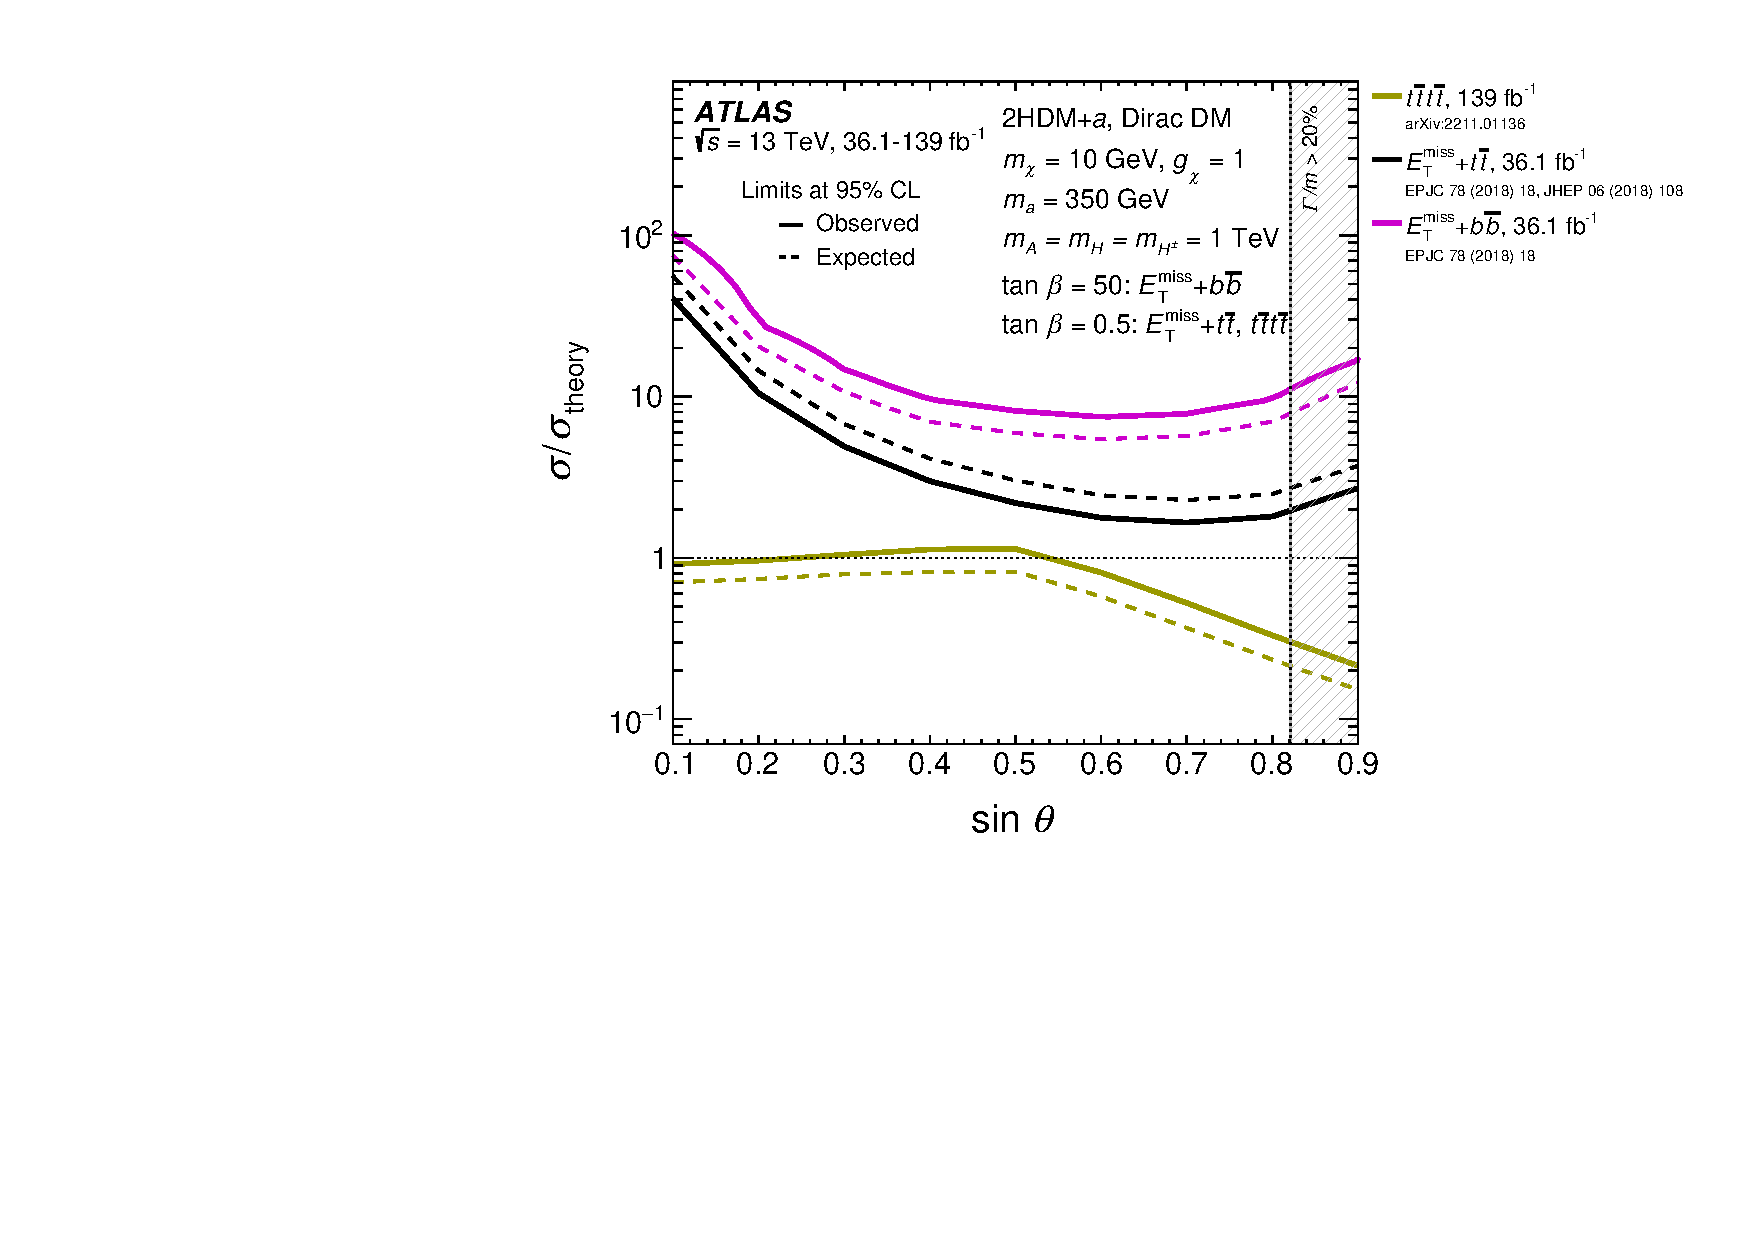
\includegraphics[width=\linewidth]{figures/fig_07d.pdf}
        \caption{}
        \label{fig:result-sint-scan-d}
    \end{subfigure}
    \caption{Observed and expected exclusion limits at $95\%$ CL for the \thdma as a function of $\sint$ plane evaluated under benchmark scenarios 4. In subfigures (a) and (b), the results are derived at $\tanb=1$, while in (c) and (d) they are derived at $\tanb=0.5$ or $\tanb=50$. (a) and (c) represent the sensitivity at low pseudo-scalar mass, in particular $\mA=600$ GeV and $\ma=200$ GeV, and (b) and (d) the high-mass regime, namely $\mA=1.0$ TeV and $\ma=350$ GeV. The combined exclusion is shown along with individual searches. In all subfigures, a dashed grey region indicates the region where the width of any of the Higgs boson exceeds $20\%$ of its mass \cite{2hdma_comb}. }
    \label{fig:result-sint-scan}
\end{figure} 

For the low-mass hypothesis at $\tanb=1.0$, the most stringent limits in the region of medium to high values of $\sint$ are set by the $\monozll$ and $\monohbb$ searches. The sensitivity of the former increases monotonically with $\sint$, as the cross-section of both non-resonant and resonant production mechanisms, illustrated in figures \ref{fig:hbb-signature} and \ref{fig:zll-signature}, grows with $\sint$. On the other hand, the production diagrams contributing to the $\met+h$ signature show a different dependence on $\sint$, as discussed in references \cite{Bauer:2017ota,EXOT-2017-32}. The relative contributions of each diagram are further affected by the different selections employed by the $\monohbb$ and \monohgamgam analyses, both of which reach a the maximum sensitivity around $\sint=0.5$. 

The sensitivity of both $\monojet$ and $\met+tW$ searches also monotonically increases with $\sint$, similar to that of the $\monozll$ signature, albeit an order of magnitude lower than the latter. This is due to the smaller cross-sections of these processes. Meanwhile, the $\htb$ and $t\bar{t}t\bar{t}$ signatures see a dependence on $\sint$ compared to other signatures, since they are not directly sensitive to neutral boson production. They are particularly sensitive at small mixing angle, with the sensitivity of $\htb$ exceeding that of the $\met+Z/h$ searches at $\sint < 0.2$. 

For the high-mass hypothesis at $\tanb=1.0$, the light pseudo-scalar mass is sufficiently large to kinematically allow the $a\rightarrow t\bar{t}$ decay, introducing an additional $\sint$ dependence in the interpretation of the $\met+Z/h$ searches. Consequently, the highest sensitivity for these analyses is observed near or just below the maximal mixing condition $\theta=\pi/4$. 

In the case of the $\met +h$ searches, there is a more complex dependence on $\sint$, owing to different contributions from the resonant and non-resonant productions of the Higgs boson to the final selection of each analysis. In particular, the $\met +h(b\bar{b})$ signature displays in a broad peak at values of $\sint$ slightly below the maximal mixing. In contrast, the $\met +h(\gamma\gamma)$ shows a local sensitivity minimum around $\sint\approx 0.6$. 

The $\met + tW$ search follows a similar $\sint$ dependence as the $\monozll$ and $\monohbb$ searches, but remains approximately an order of magnitude below the combined sensitivity. On the other hand, the $\met+j$ demonstrates a monotonic increase in sensitivity and reaches a level similar to that of the $\monozll$ and $\monohbb$ searches at large $\sint$. Results from the $\met+V(q\bar{q})$ search are shown for completeness \cite{EXOT-2017-32}.

Alternative values $\tanb=0.5$ $\tanb=50$ are considered for Scenario 4 to illustrate the strong dependence of the exclusion limits on $\tanb$, particularly in searches that are sensitive to the Yukawa couplings of the neutral Higgs bosons and the mediator to fermions in a Type-II 2HDM. At low $\tanb$, the scalar and pseudo-scalar states couple primarily to top quarks, whereas at high $\tanb$, they predominantly couple to bottom quarks. Therefore, the results of the $t\bar{t}t\bar{t}$ search are shown for $\tanb=0.5$. The sensitivity of this search is generally higher in the low-mass scenario relative to the high-mass counterpart, mainly due to the reduced production cross-section of the heavy Higgs bosons $A/H$ at higher $m_{A/H}$. However, in the high-mass scenario, an enhancement in sensitivity is observed for $\sint > 0.5$, and attributed to the increased $a/A$ mixing and the fact that the mediator mass is sufficiently large to kinematically allow a decay into a pair of top quarks. At the same time, the mediator mass remains significantly below the masses of the heavy Higgs bosons, leading to the $t\bar{t}t\bar{t}$ signal cross-section being dominated entirely by $t\bar{t} + a (t\bar{t})$ production. 

For completeness, results from the $\met+t\bar{t}$ and $\met+b\bar{b}$ searches reported in reference \cite{EXOT-2017-32} are included for $\tanb=0.5$ and $\tanb=50$, respectively.

\subsection{Scenario 5: Variation of \texorpdfstring{$\mchi$}{TEXT}}

In Figure \ref{fig:result-mX-scan}, the sensitivity of various searches as a function of the fermion dark matter mass $\mchi$, which has the strongest impact on the relic density predicted by the \hdma, is shown. 
The sensitivity is evaluated as the observed exclusion limit on the ratio of the excluded cross-section to the nominal cross-section of the signal model. The relic density is overlaid on the plot as a long-dashed line. A notable feature of the relic density occurs around $\mchi=\ma/2=200$ GeV, known as the $a$-funnel region, where the predicted density is depleted by the resonant enhancement of the process $\chi\bar{\chi}\rightarrow a\rightarrow \mathrm{SM}$ \cite{Djouadi:2005dz,Bagnaschi:2015eha,2HDMWGproxi}. A second resonant, occurring at $\mchi=\mA/2=500$ GeV, corresponding to a second funnel region, is not fully covered within the probed $\mchi$ range but nevertheless visible as a decrease in the predicted relic density for $\mchi >400$ GeV. For $\mchi >200$ GeV, the relic density reaches a plateau due to the increase in annihilation cross-section of the DM particles near the kinematic threshold of the processes $\chi\bar{\chi}\rightarrow t\bar{t}$ (if $\mchi > m_t$) and $\chi\bar{\chi}\rightarrow ah$ (if $\mchi > (\ma+m_h)/2$). 

\begin{figure}[h!]
    \centering
    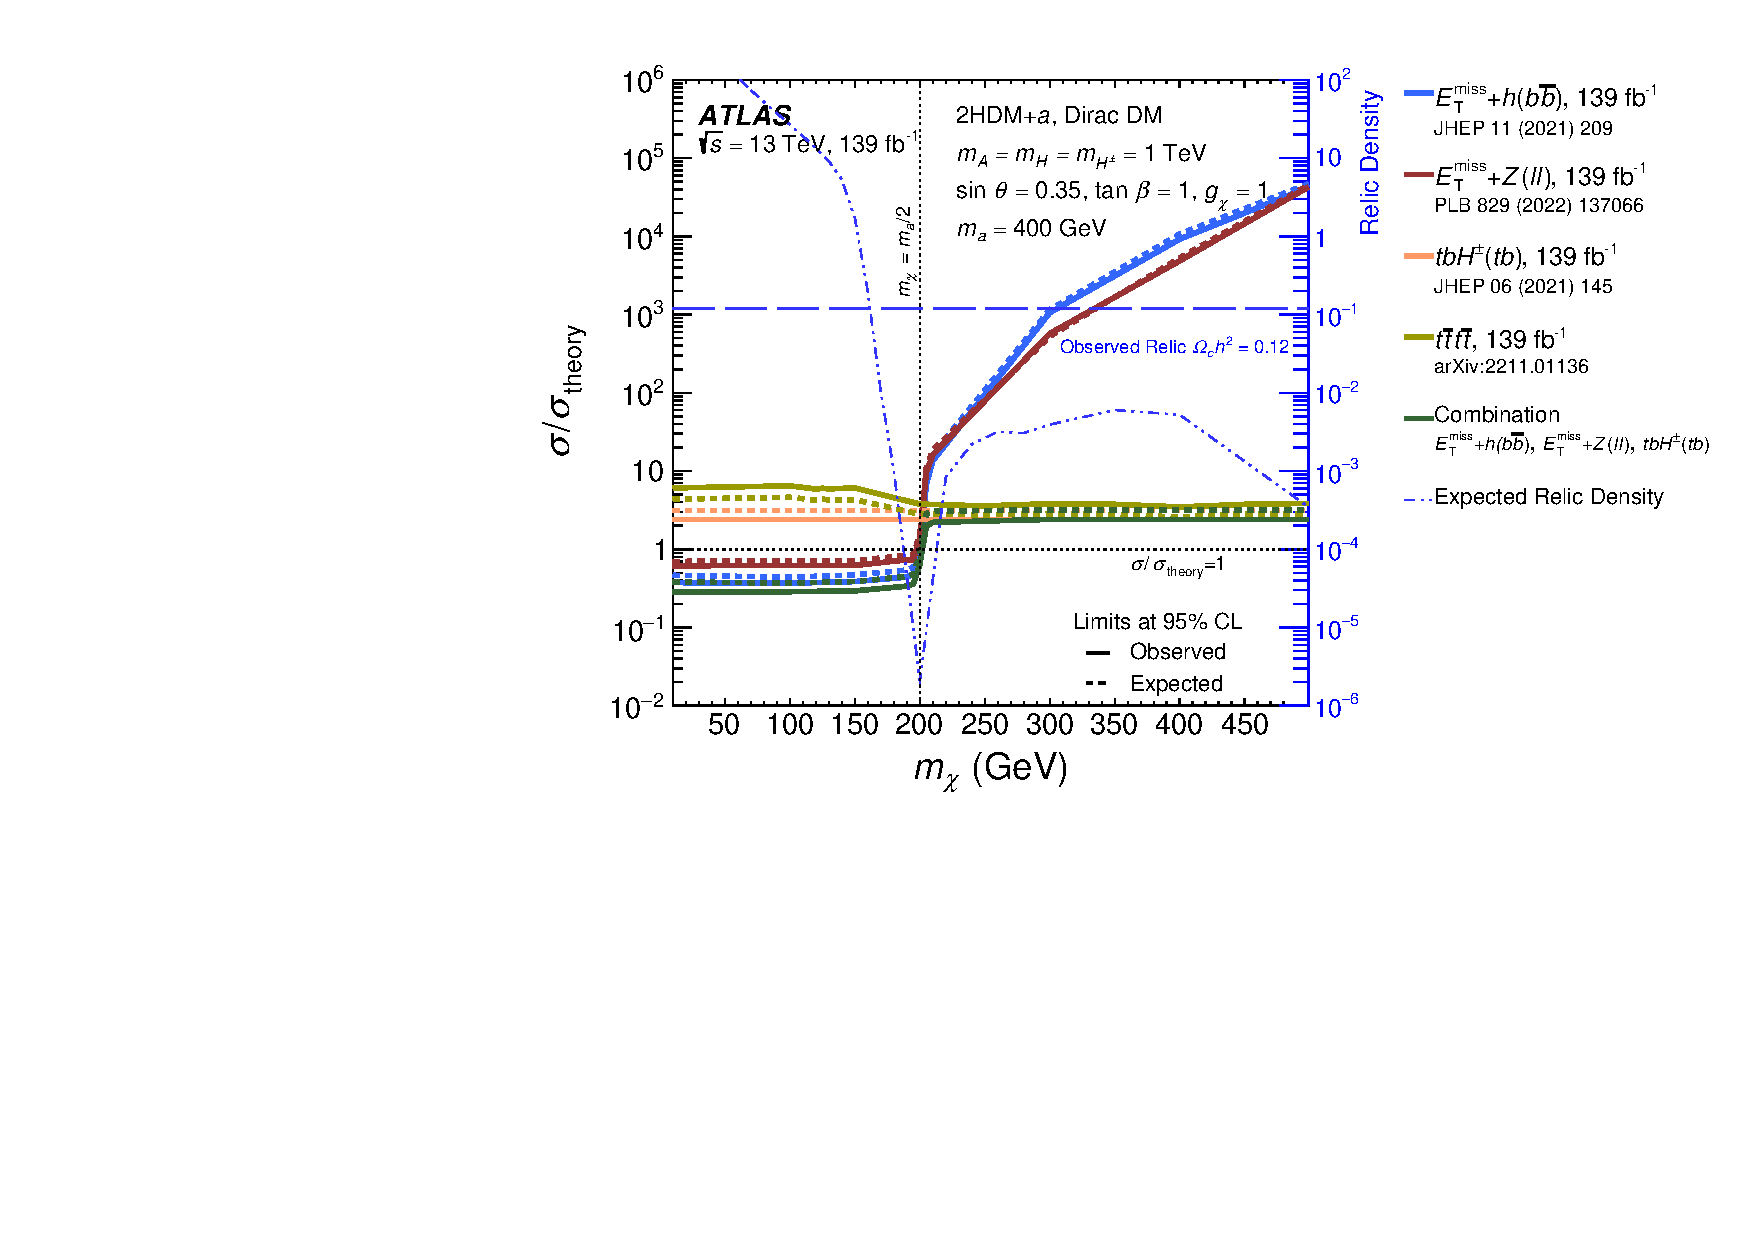
\includegraphics[width=0.6\linewidth]{figures/fig_08.pdf}
    \caption{Observed and expected exclusion limits at $95\%$ CL for the \thdma as a function of the dark matter particle mass $\mchi$ evaluated under benchmark scenario 5 following $\mA=1.0$ TeV, $\ma=400$ GeV, $\tanb=1.0$, and $\sint=0.35$. The limits are expressed in terms of the ratio of the excluded cross-section to the nominal cross-section of the signal model. The results from several individual searches are shown along with the combined limits. The relic density for each $\mchi$ assumption, calculated with \textsc{MadDM}~\cite{Ambrogi:2018jqj}, is superimposed on the plot in dashed line \cite{2hdma_comb}. }
    \label{fig:result-mX-scan}
\end{figure} 

For all considered signatures, the sensitivity becomes independent of $\mchi$ as long as the pseudo-scalar mediator, whose mass is fixed at 400 GeV in this benchmark scenario, can decay into a pair of DM particles. The most stringent constraints in the region where $\mchi<200$ GeV are provided by the $\monozll$ search. Together with the $\monohbb$, it excludes this part of the parameter space. However, at higher DM masses, the sensitivity of the $\met+Z/h$ searches rapidly decreases, while that of the $\htb$ and $t\bar{t}t\bar{t}$ searches remains largely constant. This is because the corresponding leading-order signal processes do not involve the DM particle $\chi$, rendering their signal cross-sections independent of $\mchi$. 

For $\mchi>\ma/2$, the $\htb$ search provides the strongest constraints, probing cross-sections as low as $\sigma =2\sigma_{\mathrm{theory}} - 3\sigma_{\mathrm{theory}}$. None of the searches exclude the \thdma in this mass range under the chosen benchmark scenario. It is possible to match the observed relic density for $\mchi=170$ GeV without changing the collider phenomenology, though this mass value is disfavored by the considered analyses. 

It is important to emphasize that the relic density considerations primarily serve as a tool to assess \thdma model predictions in the context of cosmological observations. They should not be interpreted as strict constraints on the model parameters, as the values of the parameters producing the correct relic density could shift if the model is modified to include additional physics at high-energy scales or if an alternative cosmological history is assumed.

\subsection{Scenario 6: \texorpdfstring{$\ma -\mchi$}{TEXT} plane}

Figure \ref{fig:result-ma-mX-scan} presents exclusion limits as a function of $\ma$ and $\mchi$ for Scenario 6. The $\hlrs$ searches target the region characterized by $\ma<m_h/2$ and $\ma < 2\mchi$, which kinematically allows the $h\rightarrow aa$ decay and forbids the $a\rightarrow \chi\bar{\chi}$ decay. This region is excluded almost entirely by these searches, except for two narrow bands where $\ma$ approaches the masses of the $J/\psi$ and $\Upsilon$ mesons. Searches for dimuon final states near the $J/\psi$ mass are experimentally challenging, as are searches for $h\rightarrow aa\rightarrow 4g$. The $\mu^+\mu^-\tau^+\tau^-$ final state provides some sensitivity but is not sufficient to exclude the higher mass range around $\ma=10$ GeV \cite{HIGG-2014-02}. Similarly, searches for hadronic final states are complicated by the collimation of the quark pairs, often necessitating dedicated techniques to enhance the sensitivity of signatures such as $b\bar{b}\gamma\gamma$ and $b\bar{b}b\bar{b}$. The $\hlrs$ searches lose sensitivity when $\ma>\mA/2$, as invisible mediator decays become dominant. For $\ma < m_h/2$, this region is excluded by the $\hinv$ search. For larger values of $\ma$, the region where $\ma>\mchi$ is excluded by the $\monohbb$  search up to $\ma\approx 600$ GeV. 

The remaining high-mass region is not excluded, and can be probed by searches targeting the mediator or heavy Higgs boson final states in $t\bar{t}t\bar{t}$ and $\htb$ signatures, which are currently unable to exclude $\mA=1200$ GeV.

\begin{figure}[h!]
    \centering
    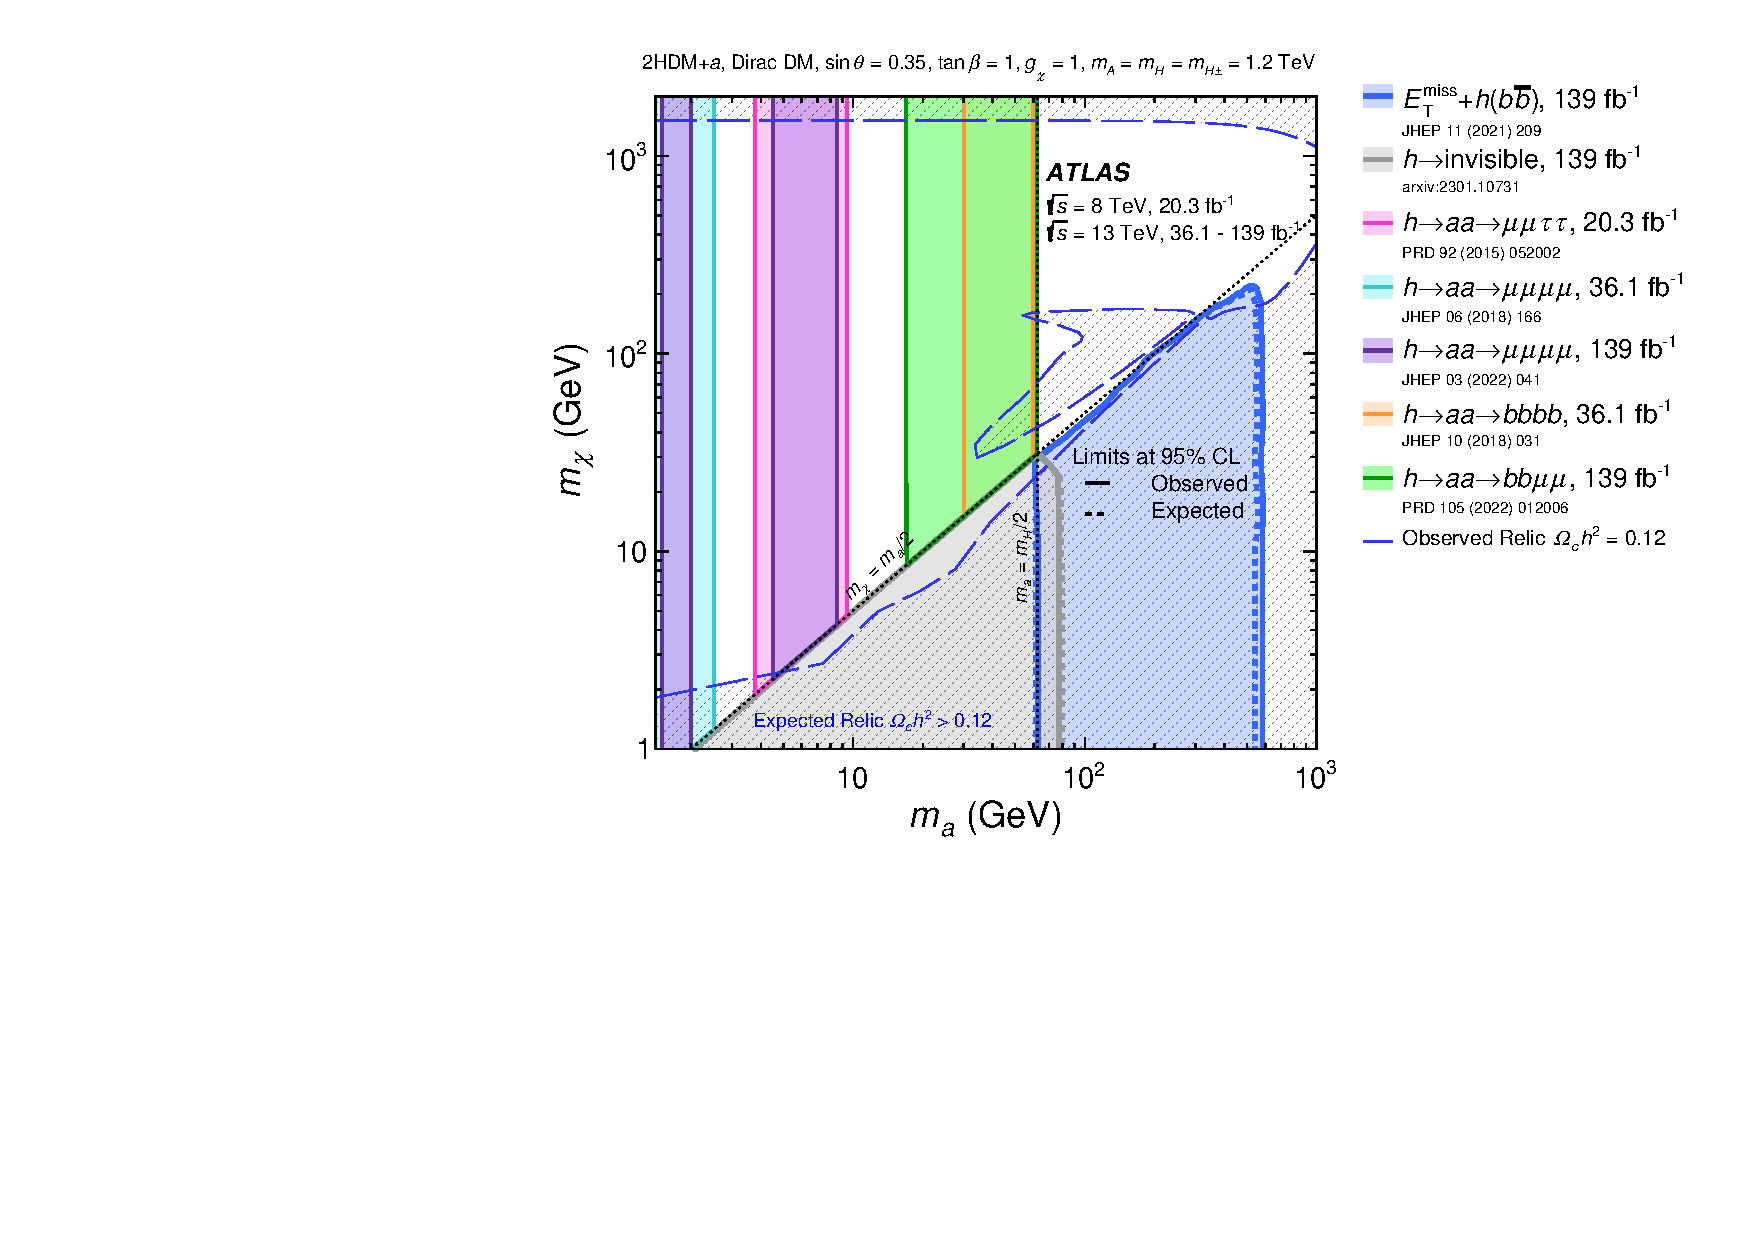
\includegraphics[width=0.6\linewidth]{figures/fig_09.pdf}
    \caption{Observed and expected exclusion limits at $95\%$ CL for the \thdma as a function of $\ma$ and $\mchi$ evaluated under benchmark scenario 6 following $\mA=1.2$ TeV, $\tanb=1.0$, and $\sint=0.35$. The relic density contour for the case $\Omega_ch^2=0.12$, calculated with \textsc{MadDM}~\cite{Ambrogi:2018jqj}, is superimposed on the plot in dashed line. The shaded regions mark the region where the model predicts a relic density greater than the observed value $\Omega_ch^2=0.12$. The island around $(\mchi\approx100, \ma\approx 100)$ GeV corresponds to the resonant enhancement of the process $\chi\bar{\chi} \rightarrow ah \rightarrow \mathrm{SM}$ that depletes the relic density \cite{2hdma_comb}. }
    \label{fig:result-ma-mX-scan}
\end{figure} 

The relic density contour for the case $\Omega_ch^2=0.12$ is overlaid on figure \ref{fig:result-ma-mX-scan} as a long-dashed line. Regions above this line at contour at low $\mchi$ and below it at high $\mchi$, with an exception of an island around $(\mchi\approx100, \ma\approx 100)$ GeV, have a predicted relic density $\Omega_ch^2 < 0.12$. 

Due to the strong Yukawa coupling, the annihilation $\chi\bar{\chi}\rightarrow t\bar{t}$ is highly efficient. However, in regions of small DM mass $(\mchi < m_t$, the decay is kinematically forbidden, often leading to an overabundance of relic density unless alternative annihilation mechanisms are available. Key processes that help deplete the relic density include resonant annihilation when $\mchi\approx \ma/2$, as well as other decay channels such as $\chi\bar{\chi}\rightarrow aa$, or $\chi\bar{\chi}\rightarrow ah$ when they are allowed or kinematically enhanced. For small mediator mass, annihilation into fermions, such as $b\bar{b}$, $c\bar{c}$, and $\tau\tau$ can be sufficiently efficient to compensate for their smaller couplings and deplete the relic density. Larger values of $\mchi$ can also satisfy the observed relic density, as these annihilations are suppressed. 

\section{Conclusion}

A wide range of searches for new phenomena performed by the ATLAS Collaboration are summarized and interpreted in the context of a Two-Higgs-Doublet model extended by a pseudo-scalar mediator $a$, designated \hdma. The model extends the Standard Model by introducing two Higgs doublets and an additional pseudo-scalar particle, which mediates interactions between dark matter and the SM particles. It predicts a wide variety of final states, of which the most relevant to DM searches consist of a large missing transverse energy originating from the decay of the mediator $a$ into DM particles and a mono-$X,\,(X=Z,h)$ visible signatures. The majority of searches considered in this summary are based on up to $139\,\ifb$ of proton-proton collision data at center-of-mass energy of $\sqrt{s}=13$ TeV collected by the ATLAS detector during the second run of the Large Hadron Collider. The results are in accordance with Standard Model predictions, as no significant excess is found. They are used to derive constraints on the \thdma for a diverse selection of benchmark scenarios recommended by the LHC Dark Matter Working Group previously explored, as well as several benchmark scenarios which provide insights into the rich phenomenology of the model. Three searches targeting $\monozll$, $\met+b(b\bar{b})$, and $\htb$ examine complementary regions of the parameter space, provide the most stringent constraints in many benchmark scenarios, and thus enter a statistical combination to derive an enhanced set of limits on the \hdma. 

All benchmark scenarios are simplified by assuming the mass degeneracy of the additional Higgs bosons, namely $\mA=m_{H^{\pm}}=m_H$. The combined result excludes masses of the pseudo-scalar mediator $a$ up to 560 GeV for $m_{A/H/H^{\pm}}=1.2$ TeV, $\sint=0.35$, and $\tanb=1.0$ (scenario 1a), and up to $640$ GeV for $m_{A/H/H^{\pm}}=2.0$ TeV, $\sint=0.7$, and $\tanb=1.0$ (scenario 1b). In regions of large heavy Higgs mass $(\mA)$, the $\monozll$ and $\met+b(b\bar{b})$ searches are the most sensitive. The results from this benchmark see a significant improvement over the same scan performed on $36\,\ifb$ of $\sqrt{s}=13$ TeV proton-proton collision data, which excludes values of $\ma$ up to 340 GeV for $m_{A/H/H^{\pm}}=1.0$ TeV, $\sint=0.35$, and $\tanb=1.0$. The improvement can be attributed to the full Run 2 dataset, as well as various improvements in the analysis strategies employed by individual searches, and a statistical combination of the most sensitive results.

The interpretation of the $\htb$ in the combined limits represents a novel strategy previously not considered. This signature is the most sensitive of the three combined searches in the low-$\mA$ region where $\ma>400$ GeV. It allows values of $\mA$ up to 650 GeV to be excluded across the entire range of examined $\ma$, highlighting the importance of searches not classically interpreted in the context of DM in constraining more complex models such as the \hdma. The statistical combination the $\monozll$, $\met+h(b\bar{b})$, and $\htb$ searches extends the sensitivity to the \thdma compared to that of individual analyses across different regions of the parameter space. In addition, the results of searches targeting $h\rightarrow aa \rightarrow f\bar{f} f'\bar{f}'$ are used for the first time to constrain a part of the parameter space not previously probed. Overall, these results represent the most comprehensive set of constraints on the \thdma obtained by the ATLAS collaboration to date.



\part{Track reconstruction with geometric deep learning using graph neural networks in the ATLAS Inner Tracker}
\chapter{The High Luminosity Large Hadron Collider}
% \label{chap:HL-HLC}
% \section{An overview of the Large Hadron Collider}

% exposition on 
% the general principle of the LHC
% key parameter : luminosity, how it translates to physics, 
% how to control the luminosity, current luminosity of the LHC, how much data it has derivered
% introduce the HL-LHC

At the time of writing this thesis in 2025, the LHC has been in operation for over 13 years and delivered to each of its general-purpose detectors--ATLAS and CMS--approximately $350\,\ifb$ of proton--proton collision data at a peak center-of-mass energy of $\sqrt{s}=13$ TeV. 
Table \ref{tab:lhc-int-lumi} illustrates  the energy and quantity of data collected over the LHC runs. 
An instantaneous luminosity of $2\times 10^{34} \, \mathrm{cm}^{-1}s^{-1}$ was achieved in 2018 and has been maintained until now, furnishing an integrated luminosity of $350\,\mathrm{fb}^{-1}$, well above the initial goal of $300\,\mathrm{fb}^{-1}$.

\begin{table}[h!]
    \centering
    \begin{tabular}{|c|c|c|}
    \hline
        Run & Period & Integrated luminosity $[\ifb]$ \\ \hline
        1 & 2010 -- 2012 & 29.2 \\
        2 & 2015 -- 2018 & 159.8 \\
        3 & 2022 -- 2025 & 160.4 \\ \hline \hline
        \multicolumn{2}{|c|}{Total} & 349.4 \\
        \hline
    \end{tabular}
    \caption{The integrated luminosity delivered to the ATLAS detector by the LHC as of September 2, 2024. }
    \label{tab:lhc-int-lumi}
\end{table}

Even before the nominal LHC operation, the High-Luminosity LHC (HL-LHC) project was established to fully exploit the collider's discovery potential. 
The aim is to increase the instantaneous luminosity to $5\times 10^{34} \, \mathrm{cm}^{-1}s^{-1}$, reaching up to $7.5\times 10^{34} \, \mathrm{cm}^{-1}s^{-1}$, 3.75 times higher than the current rate. 
As such, the total integrated luminosity at the end of the HL-LHC will attain $3000\,\mathrm{fb}^{-1}$, 10 times the data planned for the baseline LHC.
Increasing luminosity proportionately increases the rate of event production $\expval{N}$, since
\beq
\label{eq:hllhc:1}
\expval{N_{pp\to X}}=\mathcal{L}\sigma_{pp\to X}
\eeq
where $\mathcal{L}$ and $\sigma_{pp\to X}$ are respectively the instantaneous luminosity and the production cross-section of the final state $X$. 
For example, the production cross-section of a Higgs boson is $\sigma_{pp\to H}=50 \, \mathrm{pb}$, so the average Higgs production rate at the current luminosity $\mathcal{L} = 2\times 10^{34}\, \mathrm{cm}^{-1}s^{-1}$ is 
\beq
\label{eq:hllhc:2}
\expval{N_{pp\to H}}= [2\times 10^{34}\, \mathrm{cm}^{-1}s^{-1}] \times [50 \times 10^{-36}\, \mathrm{cm}^{-2}] = 1\, \mathrm{Hz},
\eeq
i.e. one Higgs boson produced every second.

\begin{figure}[h!]
    \centering
    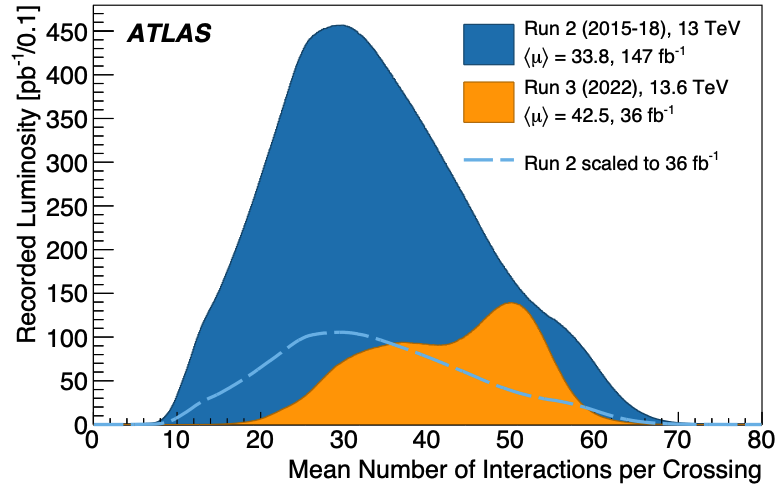
\includegraphics[width=0.65\linewidth]{figures/pileup-dist.png}
    \caption{Distribution of pile-up multiplicity $({\mu})$ in proton--proton collision at the ATLAS interaction point during Run 2 and the data taking period in 2022 of Run 3. The dashed line represents a rescaled Run 2 distribution such that its integral is the same as that of the Run 3 distribution. $\expval{\mu}$ denotes the distribution mean. Figure taken from reference~\cite{software-perf-atlas-run3}.}
    \label{fig:pileup-dist}
\end{figure}

All interactions that can occur in $pp$ collision are boosted by higher luminosity. 
The rate not only of interesting collision events, but also of soft background events increases.
The gross number of proton--proton interactions per bunch crossing, called the \textbf{pile-up multiplicity} and denoted $\mu$, can be estimated using equation \eqref{eq:hllhc:1} by noting that the total $pp$ cross-section is of order $100\,\mathrm{mb}$.
Figure \ref{fig:pileup-dist} shows the distribution of the average pile-up at the ATLAS interaction point during Run 2 and the first year of Run 3.
While pile-up primarily ranged from 20-40 in Run 2, it peaks around $\mu=50$ in a large fraction of events recorded by ATLAS in Run 3.
The HL-LHC is designed to achieve a peak luminosity of $7.5\times 10^{34} \, \mathrm{cm}^{-1}s^{-1} $, corresponding to and average pile-up of $\expval{\mu}=200$.

To prepare for this major change in operating conditions, the accelerator as well as all experiments at the LHC will undergo significant upgrades during the Long Shutdown after Run 3, between 2026 and 2029. 
In the ATLAS Collaboration, both hardware and software upgrades will take place, among which the most relevant to this thesis is the replacement of the current Inner Detector described in section \ref{subsect:inner-detector} by a new all-silicon \textbf{Inner Tracker}, commonly known as the \textbf{ITk}. 
Chapter \ref{chap:itk} describes the design and simulation of the ITk, and chapter \ref{chap:atlas-reco-chain} the current track reconstruction chain, concluding with the challenges associated with this process at high pile-up. 
This difficulty motivates the development of a novel, accelerated tracking algorithm, which constitutes the rest of this thesis.

% \section{The ATLAS Inner Tracker}



% \section{The ATLAS Inner Tracker}

% \section{A roadmap to ATLAS LH-HLC}

\chapter{The ATLAS Inner Tracker}
\label{chap:itk}
% This chapter highlights aspects of the ITk:
% \begin{enumerate}
%     \item Technical spec
%     \item Simulation (drawn from TDR)
%     \item Anything else that we need for subsequent chapters
% \end{enumerate}
The Inner Tracker (ITk) is the successor to the current Inner Detector (ID) in the High-Luminosity era.
It inherits many design features from the Pixel and SCT components of the ID, but with significant improvements in granularity, geometry coverage, material budget and expected parameter resolution. 
Understanding of its geometry and interaction with charged particles is crucial to fully simulate its detector response, extract useful information from track candidates, and interpret tracking results.
This chapter describes aspects of the ITk design and simulation, providing a foundation for the discussion in subsequent chapters. 

\section{Overview of the Inner Tracker}
\label{sect:itk-overview}

The Inner Tracker consists of two silicon-based sub-detectors, a Pixel Detector close to the interaction point (IP) and a Strip Detector at a larger radius, and, unlike the Inner Detector, without the Transition Radiation Tracker. 
They feature a total area of $180$ $\mathrm{m}^2$ with more than 5 billion readout channels, in comparison to $63$ $\mathrm{m}^2$ and 100 million channels in the ID, translating to a significant increase in granularity. 
In the barrel region, the pixel subsystem comprises five layers and the strip subsystem four layers.
Each of the endcaps is equipped with six strip rings feature a petal design and many thin pixel rings. 
The layout of the ITk, demonstrated in figure \ref{fig:itk-layout}, is optimized to provide maximal hit coverage across the pseudorapidity range. 

\begin{figure}[h]
    \begin{subfigure}[b]{0.49\textwidth}
        \centering
        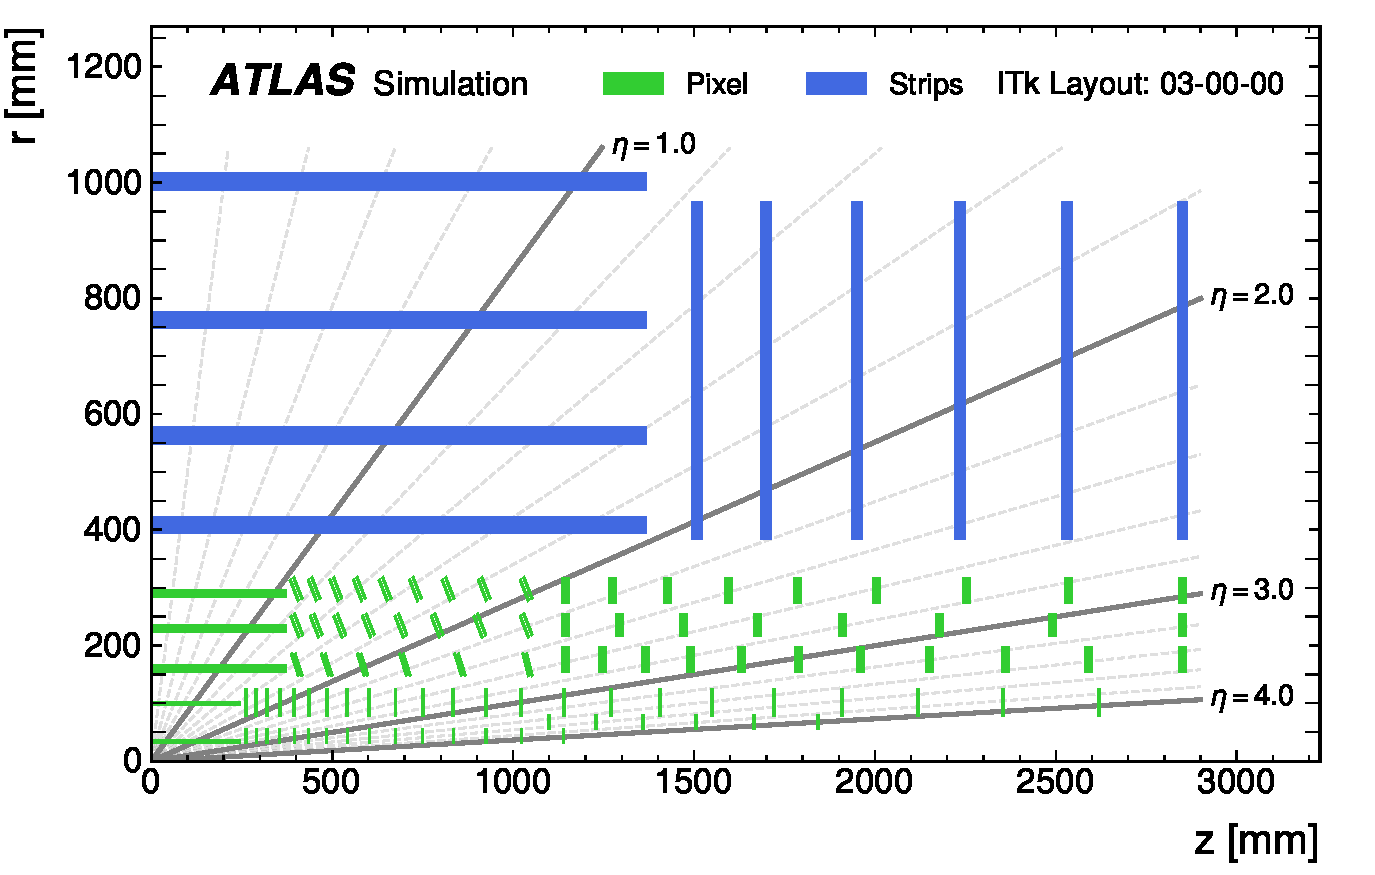
\includegraphics[width=\linewidth]{figures/itk-layout.pdf}
        \caption{}
        \label{subfig:itk-layout}
    \end{subfigure}
    \begin{subfigure}[b]{0.49\textwidth}
        \centering
        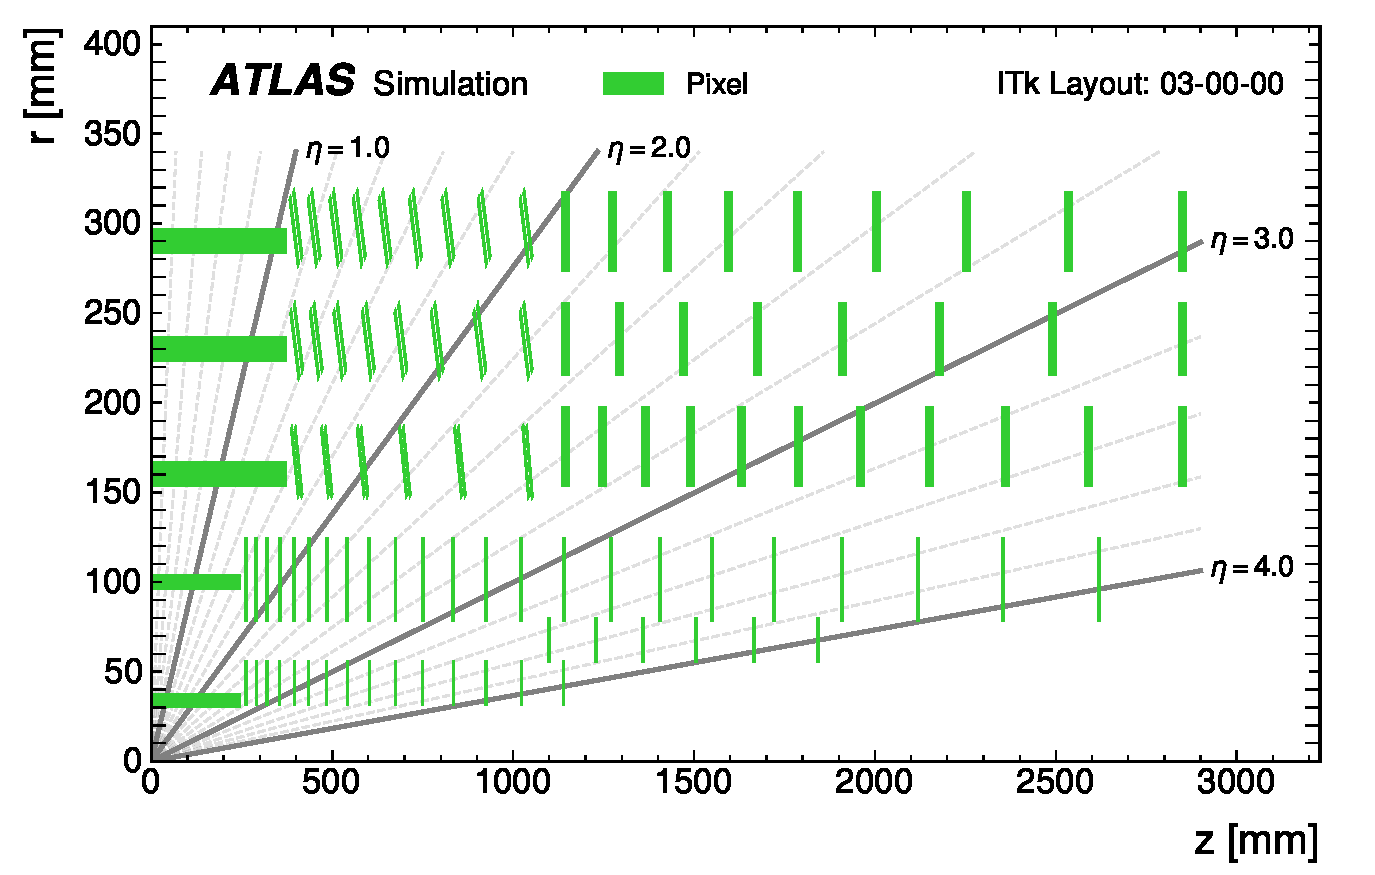
\includegraphics[width=\linewidth]{figures/itk-layout-pixel.pdf}
        \caption{}
        \label{subfig:itk-layout-pixel}
    \end{subfigure}
    \caption{A schematic view of the ITk layout (a), and of the pixel detector layout (b), both in one quadrant. Only active elements are visible in both figures. Pixel and strip elements are respectively shown in green and blue. The IP is located at the origin. The horizontal axis is parallel to the beam line, and the vertical axis is the radius measured from the IP~\cite{Aad_2025}.}
    \label{fig:itk-layout}
\end{figure}

The ITk is immersed in a solenoidal magnetic field of 2T, whose principal component lies largely along the $z$-axis. 
The bending power of the magnetic field creates a curvature in the trajectory of a charged particle, from which its transverse momentum $p_T$ is deduced. 
In addition, the ITk produces tracking measurements in close proximity to the IP, which plays an important role in impact parameter estimation, vertex fitting and subsequent pile-up mitigation.
In addition, the detector is designed to measure at least 9 hits per track in the barrel region and 13 in the endcaps, which provide strong constraints on the curvature of the track. 
Finally, pseudorapidity coverage is extended up to $\abs{\eta}=4$, in comparison to $\abs{\eta}<2.5$ in the ID. 

The ITk layout plays an important role in simulation and event reconstruction. 
It has undergone numerous refinements and evolutions since the first layout detailed in the technical design reports \cite{ATLAS-TDR-25, ATLAS-TDR-30}, with the current edition designated 03-00-00. 
All subsequent results in this document are evaluated on data simulated using this version. 

The pixel system is divided into three subsystems: the Inner System, the Outer Barrel, and the Outer Endcap. 
The Inner System (IS) encompasses the two innermost layers of the pixel detector, the first of which is located at a radius of 34 mm from the beam pipe. 
Because of its proximity to the luminous region, the IS is exposed to the highest radiation damage of the entire ITk, and is thus designed to be replaced after 2000 $\ifb$ of data has been recorded, when its modules are anticipated to deteriorate. 
The Outer Barrel (OB) radially covers the IS in the central region at larger radii, and consists of three layers of modules and three sets of endcap rings. 
As seen on figure \ref{subfig:itk-layout-pixel}, the inner rings of the OB are mounted at an incline angle to maximize the angular coverage while using less silicon, and to minimize the material length traversed by a particle having $1.0<\abs{\eta}<2.8$. 
The third subsystem, the Outer End-cap (OE), contains three sets of double-sided rings located on each side of the OB at $\abs{z}\approx 3000$ mm.

The pixel detector uses two different types of silicon sensors, namely 3D and planar sensors, depending on the radiation dose expected at different layers. 
The former is installed on the innermost layer and rings of the IS due to its radiation hardness, which is improved with respect to the 3D sensors employed in the ID. 
The rest of the pixel layers and rings uses planar sensors. 
The dimension of a pixel featured on the 3D sensor is 25 $\mu m$ in $R\phi$ direction and 100 $\mu m$ in the longitudinal direction, while the rest of the detector uses $50\times 50$ $\mu m^2$ pixels. 
The small pixel size implies a better resolved cluster shape, and subsequently improves impact parameter resolution. 
The pixel detector layout in the barrel and endcaps is summarized in tables \ref{tab:pixel-barrel-inclined-rings} and \ref{tab:pixel-endcap-rings}. 
In both tables, the triplet module features three connected read-out chips each processing electronic signals from a $2\times 2\, \mathrm{cm}^2$ sensor, and the quad module features 4 connected chips processing signals from a single $4\times4\,\mathrm{cm}^2$ sensor. 

\begin{table}[h]
    \centering
    \scalebox{0.9}{
    \begin{tabular}{|c|c|c|c|c|c|c|c|c|}
    \hline
        Barrel & Radius  & Rows of  & Flat barrel  & Incl. rings  & Incl.  & Module  & Sensor  & Sensor\\
        layer & [mm]  & sensors  & $\abs{z}$ [mm] & per row  & $\abs{z}$ [mm] & ring  & type  & dim. $[\mu \mathrm{m}^2]$ \\ \hline
        0 & 34 & 12 & 0-245 & 24 &  &  & triplets & $25\times100$\\
        1 & 99 & 20 & 0-245 & 12 &  &  & quads & $50\times50$\\
        2 & 160 & 32 & 0-372 & 18 & 380-1035 & $2\times6$ & quads & $50\times50$\\
        3 & 228 & 44 & 0-372 & 18 & 380-1035 & $2\times8$ & quads & $50\times50$\\
        4 & 291 & 56 & 0-372 & 18 & 380-1035 & $2\times9$ & quads & $50\times50$\\
        \hline
    \end{tabular}
    }
    \caption{Representative parameters of the pixel flat barrel and inclined rings in the ITk layout 03-00-00. Note that while all pixel layers have rings, only the OB features inclined rings. The fifth column provides the number of flat sensors mounted on a complete stave in the central barrel of each layer. The number of inclined rings is given by 2 $\times$ the number of rings on each of the barrel~\cite{Aad_2025}.}
    \label{tab:pixel-barrel-inclined-rings}
\end{table}

\begin{table}[h]
    \centering
    
    \begin{tabular}{|c|c|c|c|c|c|c|}
    \hline
        Ring & Radius  & $\abs{z}$ & Rings        & Sensors  & Module   & Sensor  \\
        layer& [mm]    & [mm]      &              & per ring & type     & dim. $[\mu\mathrm{m}^2]$ \\ \hline
        0    & 33.20   & 263-1142  & $2\times 15$ & 18       & triplets & $50\times50$\\
        0.5  & 58.70   & 1103-1846  & $2\times 6$ & 30       & triplets & $50\times50$\\
        1    & 80.00   & 263-2621  & $2\times 23$ & 20       & quads    & $50\times50$\\
        2    & 154.50  & 1145.5-2850  & $2\times 11$ & 32       & quads    & $50\times50$\\
        3    & 214.50  & 1145.5-2850  & $2\times 8$ & 44       & quads    & $50\times50$\\
        4    & 274.60  & 1145.5-2850  & $2\times 9$ & 52       & quads    & $50\times50$\\
        \hline
    \end{tabular}
    \caption{Representative parameters of the pixel endcaps in the ITk layout 03-00-00. The radius in the second column refers to the radius of the circle formed by the innermost point of the sensors on each ring. The number of rings is twice the number of rings on each of the barrel~\cite{Aad_2025}.}
    \label{tab:pixel-endcap-rings}
\end{table}

The strip detector is divided into two subsystems: the barrel region and two endcap regions with different arrangements of sensor modules. 
Figure \ref{fig:strip-stave-petal} shows an overview of the support structure and the arrangement of strip modules in each subsystem. 
In the barrel region, four cylindrical barrel layers surround the beam line and cover $\abs{z} < 1.4$ m. 
Each layer consists of staves running parallel to the $z$-axis, on each side of which 14 modules are mounted. 
The strips on each side of the stave are rotated with respect to the $z$-axis by $\pm26$ mrad to form a stereo angle of 52 mrad between the microstrip on the two sides. 
Since each microstrip provides a one-dimensional measurement, the stereo angle allows an estimate of a second coordinate from combining the measurements on both side of the stave. 
The strips on the two inner cylinders are 24.1 mm long and those on the outer two are 48.2 mm long, designated respectively as short- and long-strips. 
The barrel sensors are tilted in the $R\phi$ plane to allow for an overlap between neighbouring sensors which ensures detection coverage over the entire azimuthal range ($\phi$-hermeticity). 
Table \ref{tab:strip-barrel} shows the number of staves, tilt angle, and strip length on each barrel strip layer. 

\begin{figure}[h]
    \centering
    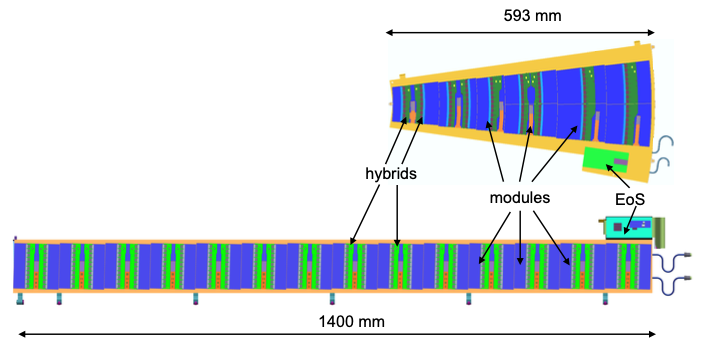
\includegraphics[width=0.8\linewidth]{figures/strip-stave-petal.png}
    \caption{Overview of the endcap petal (upper) and barrel stave (lower) in the strip detector. Sensor modules shown in blue are mounted directly on a rigid carbon-fiber sandwich structure. Only one half of a stave is shown~\cite{ATLAS-TDR-25}.}
    \label{fig:strip-stave-petal}
\end{figure}

The endcap region features six disks on each side, the outermost of which is located at $\abs{z}=3$ m. Each endcap disk is partitioned into 32 identical wedge-shaped petals, and each petal contains nine modules on each side organized into six subsegments referred to as rings (figure \ref{fig:strip-stave-petal}). The strips on each side are constructed with a stereo angle of $\pm20$ mrad with respect to the radial line that bisects the petal, achieving a total stereo angle of 40 mrad between the two sides. Because of the increasing circumferences of the petal rings, each of them has a distinct sensor geometry and electronic arrangement. These features are detailed in the Technical Design Report~\cite{ATLAS-TDR-25}.

\begin{table}[h]
    \centering
    \begin{tabular}{|c|c|c|c|c|}
    \hline
       Barrel  & Number of & Radius [mm] & Tilt           & Strip \\
       layer   & staves    &             & angle [degree] & length [mm] \\ \hline
        0      & 56         & 399 & 13 &  2.5 \\
        1       & 80        & 562 & 12 &  2.5 \\
        2       & 112       & 762 & 12 &  5 \\
        3       & 144       & 1000 & 11 & 5 \\ \hline
    \end{tabular}
    \caption{Characterization of the strip barrel, including the number of staves, radius, tilt angle, and strip length in the ITk layout 03-00-00~\cite{Aad_2025}.}
    \label{tab:strip-barrel}
\end{table}

\section{Simulation of the Inner Tracker}
\label{sect:itk-simulation}
The production of data samples used to study track reconstruction in the ITk proceeds through several steps: event generation, detector simulation using \GEANT \cite{Agostinelli:2002hh}, and digitization of simulated energy deposits. 
% The last step in the chain is the reconstruction of charged-particle tracks from the digitized data. In offline tracking, the reconstruction step is carried out by an algorithm called the Combinatorial Kalman Filter (CKF). The purpose of this work is finding a candidate replacement for the CKF which scales better under HL-LHC pile-up condition. 
Detector simulation is the costliest and the most difficult step, having to account for complex detector effects on the particle's trajectory.
Charged particles interact with the material through which they travel via several mechanisms. 
Because material interactions can change both the magnitude and direction of particle momentum, an accurate description of the material distribution in the detector is crucial to the modelling of particle trajectories as well as the extraction of track parameters from track candidates. 
Particular care was taken to describe the material at a high level of detail. 
The dimensions, location, and material of all detector elements are implemented in the simulation framework. 
The location of the material is shown in figure \ref{fig:itk-material-location}. 
The materials are defined in \GEANT in terms of their chemical composition and density.

\begin{figure}[h!]
    \centering
    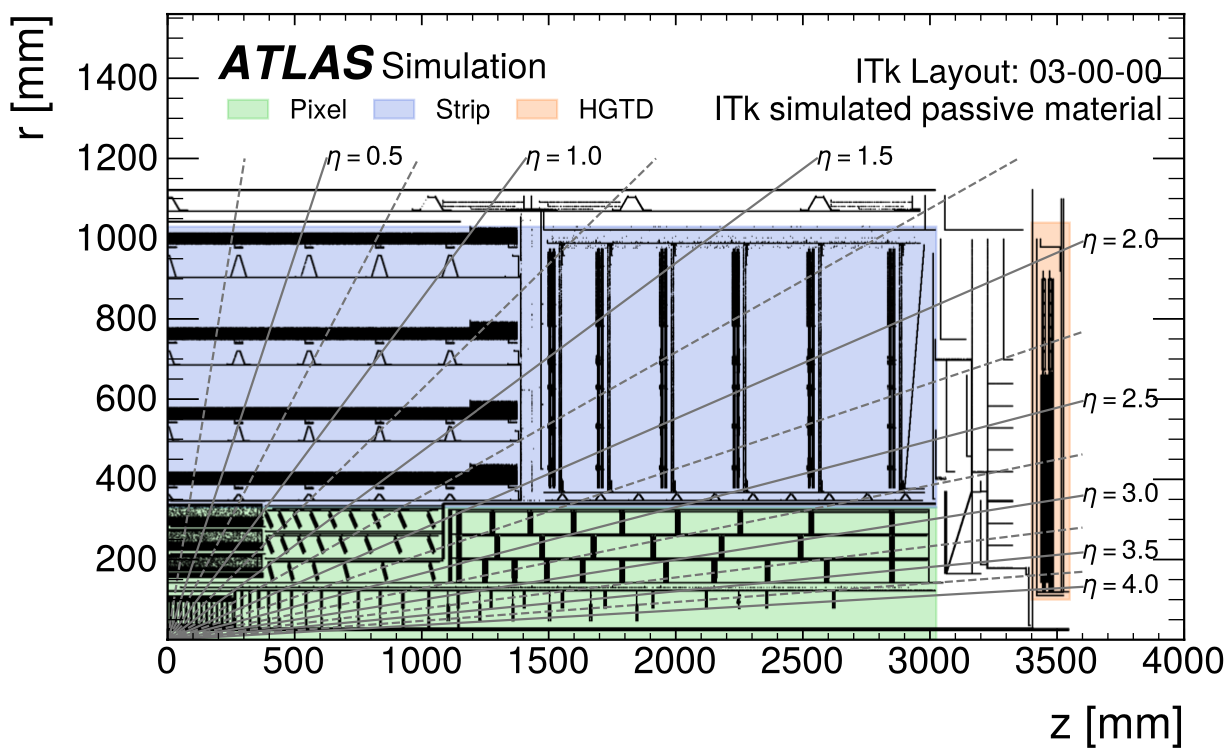
\includegraphics[width=0.75\linewidth]{figures/itk-material-location.png}
    \caption{Location of the materials for one quadrant of the ITk layout 03-00-00. The pixel subsystem is shown in green and surrounded by the strip subsystem shown in blue. The location of the materials are indicated by black regions~\cite{2HDMWGproxi}. }
    \label{fig:itk-material-location}
\end{figure}

\subsection{Simulation of the Pixel Detector }

The Pixel Detector is divided into a barrel region and two identical endcaps. The outer barrel support structure is modelled using the longeron support structure, shown in figure \ref{fig:itk-longeron}. The longeron truss structures are approximated as thin sheets of carbon fiber, and the main rails supporting the truss, accounting for 80\% of the mass, are modelled by denser materials. 

The inner barrel support structure is modelled as truss double shells, with one shell per layer. The shells are modelled as a sheet of carbon fiber behind each row of modules. The total mass of each shell in the support structure is adjusted to match the corresponding engineering estimate. The outer pixel endcaps are modelled as rings. Each layer of rings is also supported by a cylindrical carbon-fiber shell.

\begin{figure}[h!]
    \centering
    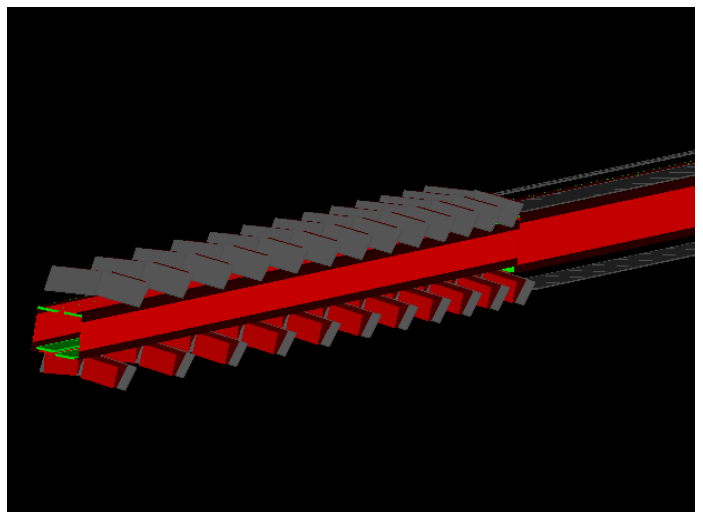
\includegraphics[width=0.5\linewidth]{figures/itk-longeron.png}
    \caption{An illustration of the \GEANT geometry model of the outer barrel longeron stave with mounted inclined and flat modules. Figure taken from reference~\cite{ATLAS-TDR-30}.}
    \label{fig:itk-longeron}
\end{figure}

Pixel modules are modelled as an active sensor volume and a front-end (FE) chip. Layer 0 of both the barrel in the endcaps features 3D pixel sensors. The active part of the sensor is implemented as a 150-$\mu m$ thick layer of silicon and the support wafer as a 100-$\mu m$ thick layer of inactive silicon. Other layers feature planar pixel sensors, modelled as 100-$\mu m$ and 150-$\mu m$ thick active silicon respectively in layer 1 and layers 2-4. 

Front-end chips are modelled as a 150-$\mu m$ thick silicon wafer, with a 1-$\mu$m thick copper layer to model its circuitry, and a Sn-Ag bump bond of 20-$\mu$m in diameter per pixel channel. The material of each component in the FE chips is homogeneously distributed throughout its corresponding volume.

\subsection{Simulation of the Strip Detector}

In the strip barrel detector, each individual part is modelled separately, with masses and material compositions reflecting the mechanical designs. In the strip endcaps, materials and objects in close proximity with each other are not individually modelled, but instead as one homogeneous block of material adjusted to have the same radiation length as calculated based on engineering designs. Figure \ref{fig:itk-strip} displays the \GEANT  geometry model of barrel staves and endcap petals in the Strip detector. 

\begin{figure}[h!]
    \begin{subfigure}[b]{0.49\textwidth}
        \centering
        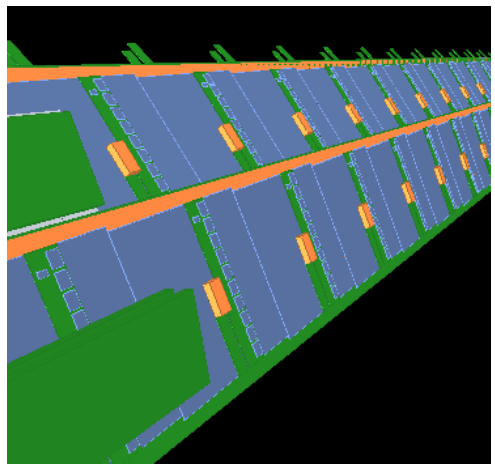
\includegraphics[width=\textwidth]{figures/itk-barrel-staves.png}
        \caption{}
        \label{subfig:itk-barrel-staves}
    \end{subfigure}
    \begin{subfigure}[b]{0.49\textwidth}
        \centering
        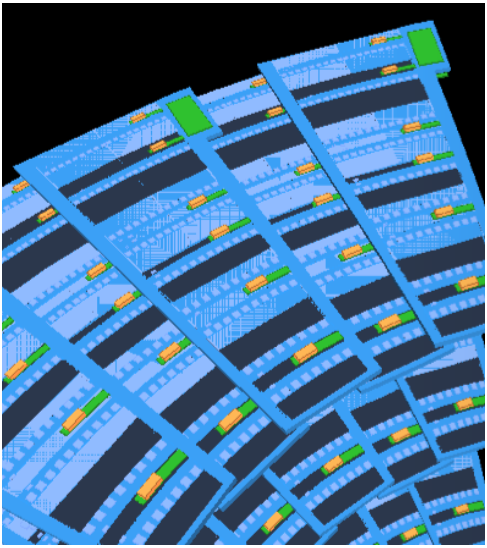
\includegraphics[width=\textwidth]{figures/itk-endcap-petals.png}
        \caption{}
        \label{subfig:itk-endcap-petal}
    \end{subfigure}
    \caption{Displays of the \GEANT geometry model of the strip barrel staves (left) and the endcap petals (right). Figure taken from reference~\cite{ATLAS-TDR-30}.}
    \label{fig:itk-strip}
\end{figure}

The global support of the detector in both the barrel and the endcaps is modelled in detail. Components include stave cooling pipes, carbon-foam, facesheets, cable bus, hybrids, and FE ASICs. Endcap sensors are individually modelled, while other components are modelled as a single edge-shaped object sandwiched between two silicon layers and uniformly filled with a generic material. The density of the material is adjusted to provide a radiation length of 0.02 $X_0$ per substructure. 

\section{Particle interaction with detector material}
\label{sect:material-effects}

An important aspect of realistic detector simulation as well as track reconstruction is the treatment of interactions between high-energy particles and the materials they traverse. 
For charged particles at the energy range relevant to the Inner Tracker, these interactions are dominated by two processes: (i) inelastic collisions with atomic electrons, and (ii) elastic scattering against atomic nuclei. 
In turn, they result in two primary effects: (1) a loss in energy by the particle, and (2) a deflection from the original direction of incident.  
Of the two electromagnetic processes, inelastic collisions are responsible for the greater part of the energy loss from heavy particles in matter. 
Each collision transfers but a tiny fraction of the particle's energy to the incident atom, causing an ionization or excitation of the latter\footnote{To demonstrate the scale of each energy loss, note that atomic excitations are often measured in eV, while particle energy is often given in MeV or GeV.}. 
However, the number of collisions encountered by a particle per unit path length in dense materials is typically large enough that a non-negligible amount of its energy is lost to the environment. 

\subsection{Energy loss of heavy particles}\label{subsect:e-loss-heavy}

The probability of an inelastic collision is described by the quantum mechanical scattering amplitude calculated for the corresponding process. 
In a macroscopic path length, a particle undergoes so many collisions that the distribution of total energy loss sharply peaks around an average value. 
Therefore, it is sufficient to compute the average energy loss per unit length, also called the stopping power or $\frac{dE}{dx}$. 
The stopping power of a material on an incident particle in the momentum range relevant to the ITk is given by the Bethe-Bloch formula \cite{Zyla:2020zbs}
\begin{equation}
    \label{eq:6.1}
    -\frac{dE}{dx} = 2\pi N_a r_e^2 m_e c^2 \frac{Z}{A} \left( \frac{z^2}{\beta^2}\right) \left[ \log \left( \frac{2m_e \gamma^2 v^2 W_{max}}{I^2}\right) - 2\beta^2 -\delta   \right],
\end{equation}
in which $r_e = 2.817\times 10^{-13}$ cm is the classical electron radius, $m_e$ the electron mass, $N_a$ the Avogadro's number, $I$ the mean excitation potential, $Z$ and $A$ the atomic number and atomic weight of the absorbing material, $z$ the charge of the incident particle in units of $e$, $\beta $ the $\frac{v}{c}$ ratio, $\gamma = (1-\beta^2)^{-1/2}$ the usual relativistic $\gamma$ factor, $\delta$ the density correction, and $W_{max}$ the maximum energy transfer in a single collision.
% \begin{itemize}
%     \item $r_e = 2.817\times 10^{-13}$ cm: classical electron radius, 
%     \item $m_e$: electron mass
%     \item $N_a$: Avogadro's number
%     \item $I$: mean excitation potential
%     \item $Z$: atomic number of absorbing material
%     \item $A$: atomic weight of absorbing material 
%     % \item $\rho$: density of absorbing material 
%     \item $z$: charge of the incident particle in $e$
%     \item $\beta $ : $\frac{v}{c}$ ratio of the particle 
%     \item $\gamma = (1-\beta^2)^{-1/2}$
%     \item $\delta$: density correction 
%     \item $W_{max}$: maximum energy transfer in a single collision.
% \end{itemize}
The maximum energy transfer depends on the ratio of the electron mass and the particle mass
\begin{equation}
    \label{eq:6.2}
    W_{max} = \frac{2m_ec^2\beta^2\gamma^2}{1+2\gamma (m_e/M) + (m_e/M)^2}.
\end{equation}
The left hand size of equation \eqref{eq:6.1} is called the mass stopping power, which varies slowly with different materials. The average energy loss per unit length is simply given by $\rho \left(  \frac{dE}{dx}\right)$. Shown in figure \ref{fig:bethe-bloch} is the mass stopping power computed for a positive muon in copper over 12 order of magnitude in muon momentum. The region corresponding to $10$ MeV $<p_{\mu ^+}< $ 100 GeV, most relevant in high-energy physics, is called the Bethe region where the stopping power is a function of $\beta$ alone. At non-relativistic energies, $\frac{dE}{dx}$ is dominated by the overall $1/\beta^2$ factor (note the logarithmic scale in the vertical axis of \ref{fig:bethe-bloch}). The stopping power reaches a minimum at $\beta\gamma\approx 3$, and slowly rises thanks to the logarithmic dependence up to $\beta\gamma = 1000$, a range equivalent to a muon momentum of $1-100$ GeV. This minimum is broad and almost the same for all particles of the same charge. For this reason, particles at this point are called ``minimum-ionizing".  
\begin{figure}[h!]
    \centering
    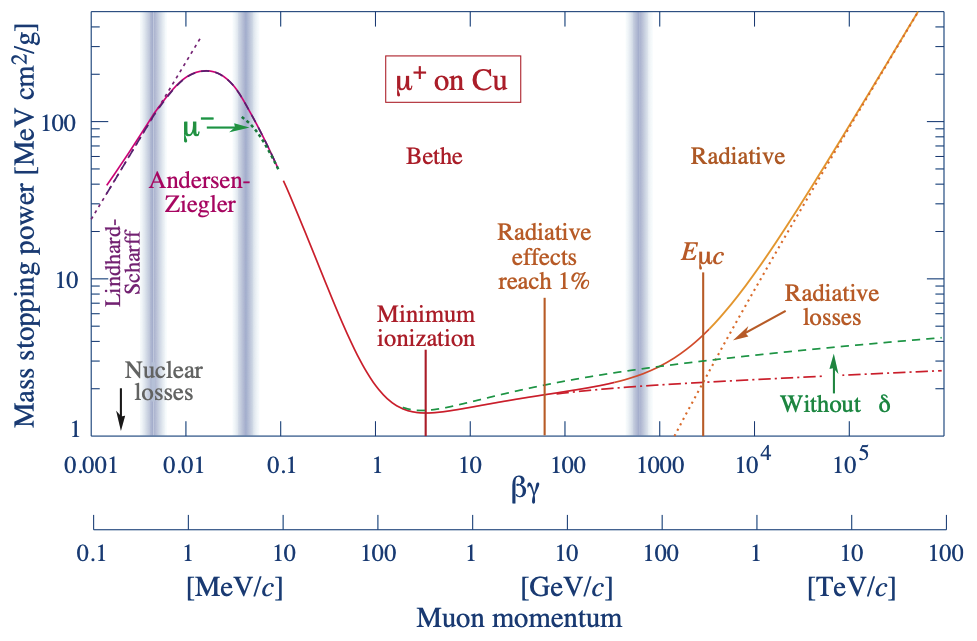
\includegraphics[width=0.9\linewidth]{figures/bethe-bloch.png}
    \caption{The mass stopping power of positive muons in copper as a function of the muon momentum spanning nine orders of magnitude. The solid curves indicate the total stopping power of all dissipative effects. The region of interest in HEP ranges from 100 MeV to 100 GeV, well within the so-called Bethe region, in which the stopping power is strongly dependent on $\beta$ (see text for definition). Figure taken from reference~\cite{Zyla:2020zbs}.}
    \label{fig:bethe-bloch}
\end{figure}

The stopping power in equation \eqref{eq:6.1} is computed for pure elements. A non-elemental material can be considered as a mixture of elements, whose stopping power is approximated by a weighted mean of $\frac{dE}{dx}$ over the elements in the compound. The weight is given by the fraction of electrons contributed by each element. In particular, the average mass stopping power is
\begin{equation}
    \label{eq:6.3}
    \frac{dE}{dx} = \sum_i w_i\left( \frac{dE}{dx} \right)_i, \quad \quad w_i = \frac{a_i A_i}{\sum_j a_j A_j}
\end{equation}
where $a_i$ is the number of atoms in the $i$-th element, and $A_i$ the atomic weight. Knowing the stopping power of each element in a material and the molecular composition, one can easily compute the mean energy loss of an incident particle given its momentum. 

Because of the statistical nature of inelastic collisions, the amount of energy deposited by a particle fluctuates around the mean calculated in equation \eqref{eq:6.1}. 
In a relatively thick absorber, the number of collisions is large, and, assuming each collision results in a small energy loss $\delta E$, such that the particle velocity stays constant, the stopping power $\frac{dE}{dx}$ negligibly varies throughout the particle's path.
The total energy loss is thus the sum of a large number of independent identically distributed random energy losses, which approaches a Gaussian as $N\rightarrow \infty$
\begin{equation}
    \label{eq:6.4}
    f(\Delta E; x) = \frac{1}{\sqrt{2\pi}\sigma } \exp \left[ \frac{-(\Delta E - \expval{\Delta E})^2}{2\sigma ^2} \right], \quad\quad \expval{\Delta E} = \int_0 ^ {x} \left(\frac{dE}{dx'} \right)dx'.
\end{equation}
with variance 
\begin{equation}
    \label{eq:6.5}
    \sigma = 0.1569 \rho \left( \frac{Z}{A} \right) \frac{1-\beta^2/2}{1-\beta^2} x.
\end{equation}

\subsection{Energy loss of electrons and positrons}
\label{subsect:e-loss-electron}
Light charged particles such as electrons and positrons undergo collisional energy loss in matter, just like heavy particles. However, because of their small mass, electromagnetic radiation in the electric field of atomic nuclei becomes a significant contribution to their overall rate of energy loss
\begin{equation}
    \label{eq:6.6}
    \left ( \frac{dE}{dx} \right) = \left ( \frac{dE}{dx} \right)_{rad} + \left ( \frac{dE}{dx} \right) _{col},
\end{equation}
in which $\left ( \frac{dE}{dx} \right)_{rad}$ is the radiative component and $\left ( \frac{dE}{dx} \right) _{col}$ the collisional component already described.

Even though the mechanism of collisional loss remains the same, because their mass is small, light particles could get deflected significantly from the original direction of incident. 
In addition, the collision occurs between identical particles, so several modifications to the Bethe equation are needed, starting with the maximum energy transfer $W_{max} = T/2$ where $T$ is the kinetic energy of the incident particle. The collisional stopping potential becomes
\begin{equation}
    \label{eq:6.7}
    -\left( \frac{dE}{dx}\right)_{col} = 2\pi N_a r_e^2 m_e c^2 \frac{Z}{A} \left( \frac{1}{\beta^2} \right) \left[ \log \frac{\tau^2 (\tau +2)}{2(I/m_ec^2)^2} + F(\tau) -\delta \right], \quad \quad \tau = \frac{T}{m_e c^2}
\end{equation}
where the function $F(\tau)$ modifies the $\beta^2$ term in equation \eqref{eq:6.1} to account for the interaction between identical particles, resulting from crossing Feynman diagrams:
$$
    F_{e^-}(\tau) = 1-\beta^2 + \frac{\tau^2 / 8 - (2\tau +1)\ln 2}{(\tau +1 )^2},
$$
and 
$$
    F_{e^+}(\tau) = 2\ln 2 - \frac{\beta^2}{12}\left( 23 + \frac{14}{\tau+2} + \frac{10}{(\tau+2)^2} + \frac{4}{(\tau + 2)^3} \right).
$$

Qualitatively, the radiative cross-section of bremsstrahlung is proportional to the inverse square of particle mass. Therefore, being far lighter than any other particle, electrons and, to a much lesser extent, muons lose a significant portion of their energy to this phenomenon. The radiative contribution to the mass stopping power can be written as
\begin{equation}
    \label{eq:6.8}
    -\left( \frac{dE}{dx}\right)_{rad} = \frac{N_a}{A}E\Phi_{rad},
\end{equation}
where $\Phi_{rad}$ is the total radiative cross section, approximated by 
\begin{equation}
    \label{eq:6.9}
    \Phi_{rad} = 4Z^2(e^2/m_ec^2)^2\alpha^2 \left [ \ln (183Z^{-1/3} ) + \frac{1}{18} - f(Z) \right],
\end{equation}
where $f(Z)$ is a small correction to the Born approximation accounting for the Coulomb interaction between the electron and the nucleus. 

It is straightforward to compare the two contributions of the total stopping power. Figure \ref{fig:rad-vs-col} demonstrates the the radiation and collisional energy losses for electron in copper as functions of the electron energy. Bremsstrahlung takes effect starting at 15 MeV, and at energy above a critical value of $\approx 25$ MeV, its contribution quickly dominates the total energy loss. This observation is due to the fact that collisional loss rises logarithmically with energy, whereas radiative loss scales linearly, evidenced by equations \eqref{eq:6.7} and \eqref{eq:6.8}. In the energy range from $1-100$ GeV relevant to the ITk, the electron stopping power is composed almost entirely of radiative loss. 

\begin{figure}[h!]
    \centering
    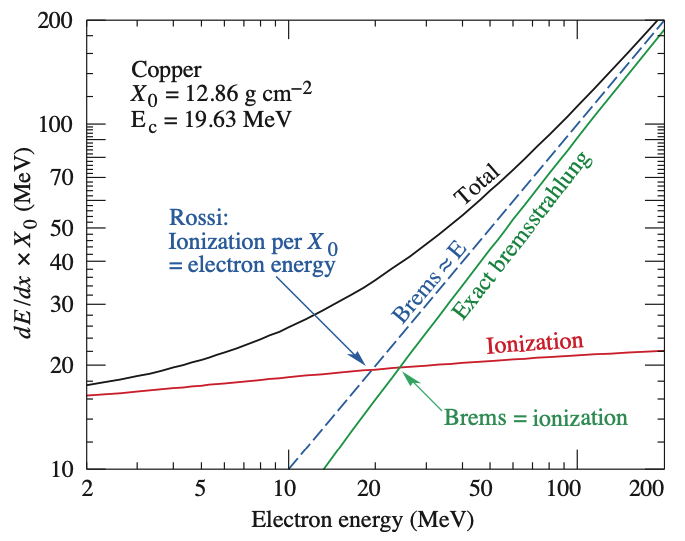
\includegraphics[width=0.65\linewidth]{figures/rad-vs-col.png}
    \caption{Contribution of radiative and collisional components in the total energy loss of electrons in copper as functions of electron energy. At a critical value $E_c=19.63$ MeV, radiative loss becomes the dominant mechanism. The energy range of electrons in HEP detectors is well within the Bremsstrahlung regime.}
    \label{fig:rad-vs-col}
\end{figure}
The critical energy at which the both components contribute equality to the total energy loss for a material is approximated by 
\begin{equation}
    \label{eq:6.10}
    E_c \,(\mathrm{MeV}) = \frac{800}{Z+1.2}
\end{equation}

It is evident that the material energy loss of electrons and positrons is characterized by the Bremsstrahlung cross section. 
In practice, it is more convenient to characterize a material by its radiation length $X_0$, defined as the distance over which the average electron energy is reduced by a factor of $1/e$ due to radiation loss. 
Equation \eqref{eq:6.8} can be rewritten as 
\begin{equation}
    \label{6.11}
    - \rho\left( \frac{dE}{dx}\right)_{rad} \frac{1}{E} = \frac{N_a\rho}{A} \Phi_{rad} = N\Phi_{rad} = \frac{1}{X_0}
\end{equation}
or 
\begin{equation}
    \label{eq:6.12}
    \boxed{E = E_0 \exp\left( -\frac{x}{X_0} \right)},
\end{equation}
where $N$ is the volumetric density of atomic nuclei in the material.

In the ITk, material thickness is described in units of radiation length. 
Figure \ref{subfig:itk-rad-len} shows the material thickness traversed by a straight track as a function of its pseudorapidity. 
Obviously, charged particles move in mostly helical orbits, whose curvature depends on the transverse momentum, because of the magnetic field, and thus the actual material length traversed by the particle is obtained by numerical integration. 
The central region has very little material, resulting from the light design of the sensor support. 
At higher $\eta$, a particle travels through progressively more layers and thus experiences almost linearly increasing material thickness. 
The largest contribution to the total radiation length comes from pixel services and cooling.

For comparison, the material depth of the ID in Run 2, including the Pixel, SCT and TRT, is shown in figure \ref{subfig:id-rad-len}, and expected material thickness traversed by a particle until it reaches the minimum number of hits required for track reconstruction in figure \ref{subfig:rad-len-to-reco}. 
The linear ITk material budget is significantly smaller than that of the ID in the forward region, despite having more layers and better eta coverage. 
This is due to the adoption of serial powering in the ITk, among other design optimizations. 
A realistic particle experiences up to 50\% more material before reaching the minimum number of hits for $\eta<1.5$ in the ITk than in the ID. 
Note, however that ID tracks are required to have only 8 hits in this region, compared to 9 hits for an ITk track. 
Beyond this point, the ITk becomes more transparent than the ID, by up to 50\%. 

\begin{figure}[h!]
\begin{subfigure}[b]{0.47\textwidth}
    \centering
    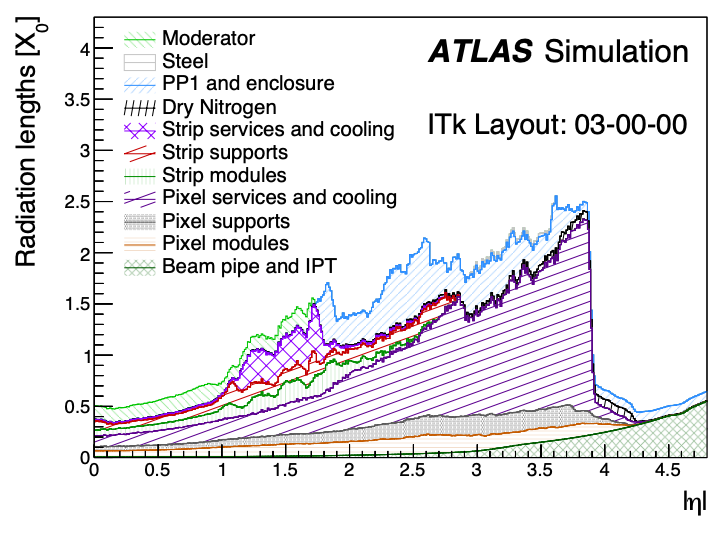
\includegraphics[width=\textwidth]{figures/itk-rad-length.png}
    \caption{ITk radiation length~\cite{Aad_2025}}
    \label{subfig:itk-rad-len}
\end{subfigure}
\begin{subfigure}[b]{0.51\textwidth}
    \centering
    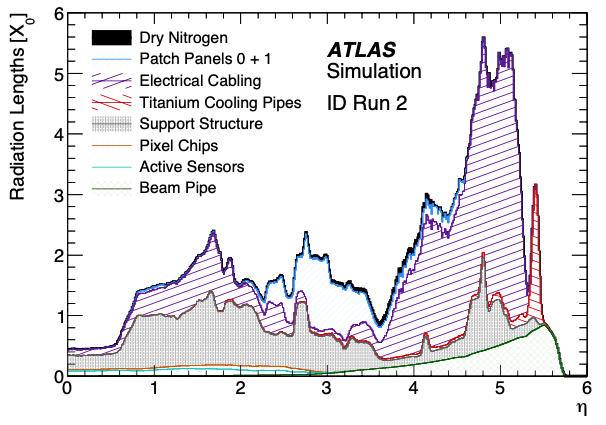
\includegraphics[width=\textwidth]{figures/id-rad-length.png}
    \caption{ID radiation length \cite{ATLAS-TDR-25}}
    \label{subfig:id-rad-len}
\end{subfigure}
\begin{subfigure}[b]{\textwidth}
    \centering
    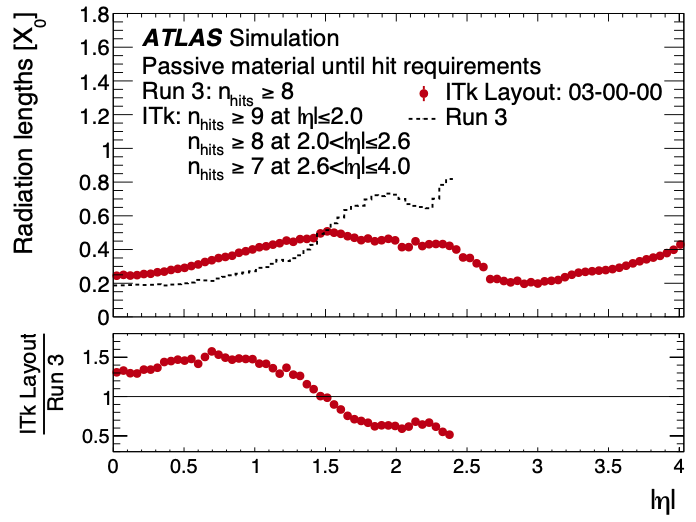
\includegraphics[width=0.5\textwidth]{figures/rad-length-to-reconstruct.png}
    \caption{Radiation length to reach reconstructible number of hits~\cite{Aad_2025}}
    \label{subfig:rad-len-to-reco}
\end{subfigure}
    \caption{Integrated material budget encountered on a particle's path in unit of radiation length as a function of pseudorapidity based on (a) the ITk and (b) the ID. The particle assumes a straight trajectory from the origin. (c) is a comparison between the amount of material that must be traverse before the particle accumulates enough hits to be deemed reconstructible.}
    \label{fig:rad-len}
\end{figure}

% A full simulation of particle trajectories takes into account the spatial material distribution and the initial value of particle momentum. The mean energy loss is numerically integrated from 
\subsection{Multiple Coulomb scattering}\label{subsect:multi-scat}

In addition to inelastic collision and radiation, charged particles undergo a large number of small-angle elastic scattering due to Coulomb interaction with atomic nuclei. 
Coulomb scatterings are governed by the Rutherford formula for non-relativistic collision, and the Mott formula for the relativistic counterpart. 
In both formulae, the scattering cross-section follows 
\begin{equation}
    \label{eq:6.13}
    \frac{d\sigma}{d\Omega} \propto \frac{1}{\sin^4 (\theta/2)}
\end{equation}
which favours a small scattering angle $\theta$. Assuming the material is sufficiently thick and the energy transfer to the nuclei is negligible, the particle suffers a large number of small deflections.
The net effect can therefore be statistically represented by a probability distribution function of the total deflection which depends on the material thickness. 
A rigorous treatment of multiple scattering is complicated. 
Among the most commonly used approximations is the theory of Molière \cite{Moliere:1947, Moliere:1948zz}, valid for the scattering of fast charged particles. 
The theory was expanded by Bethe~\cite{bethe:1953} and later Scott~\cite{scott:1963} to account for Coulomb interactions with atomic electrons. 
Although it agrees well with data, especially at small angles and large target nuclear numbers, it relies on an unwieldy series expansion and is therefore inconvenient to use. 
Rossi and Greisen~\cite{Rossi_Greisen_1941} developed a simple estimate of the root-mean-square scattering angle, which was improved by Highland~\cite{Highland_1975} and Lynch and Dahl~\cite{Lynch_Dahl_1991} to obtain the RSM width of the projected scattering angle distribution on a plane
\begin{equation}
\label{eq:6.14}
    \theta_0 = \frac{13.6z\, \mathrm{MeV}}{pc\beta} \sqrt{\frac{x}{X_0}}\left[ 1 + 0.038\ln \frac{z^2(x/X_0)}{\beta^2} \right],
\end{equation}
where $p$, $\beta c$, and $z$ are the momentum, the velocity, and the charge of the incident particle. $x/X_0$ is the material thickness in radiation lengths. 
The scattering angle projected on a plane $\theta_{plane}$ can be approximated by a Gaussian centered at $\theta_{plane}=0$
\begin{equation}
    \label{eq:6.15}
    d P(\theta_{plane}) = \frac{1}{\sqrt{2\pi} \theta_0} \exp \left[ - \frac{\theta_{plane}^2}{2\theta_0^2} \right] d\theta_{plane}
\end{equation}
The total angle $\vartheta$ can be approximated by the quadratic sum of two small projected angles on orthogonal planes
\begin{equation}
\label{eq:6.16}
\vartheta^2 = \theta_{plane,x}^2 + \theta_{plane,y}^2, \quad\quad d\vartheta = d\theta_{plane,x}d\theta_{plane,y}
\end{equation}
and with the assumption that the two projected angles are independent, $\vartheta_{tot}$ is 
\begin{equation}
\label{eq:6.17}
d P(\vartheta) = \frac{1}{2\pi \theta_0^2} \exp \left[ - \frac{\vartheta^2}{2\theta_0^2} \right] d\vartheta
\end{equation}
Figure \ref{fig:multi-scat} illustrates the quantities used to describe the effect of multiple scattering. The total scattering angle is projected on a plane 

\begin{figure}[h!]
    \centering
    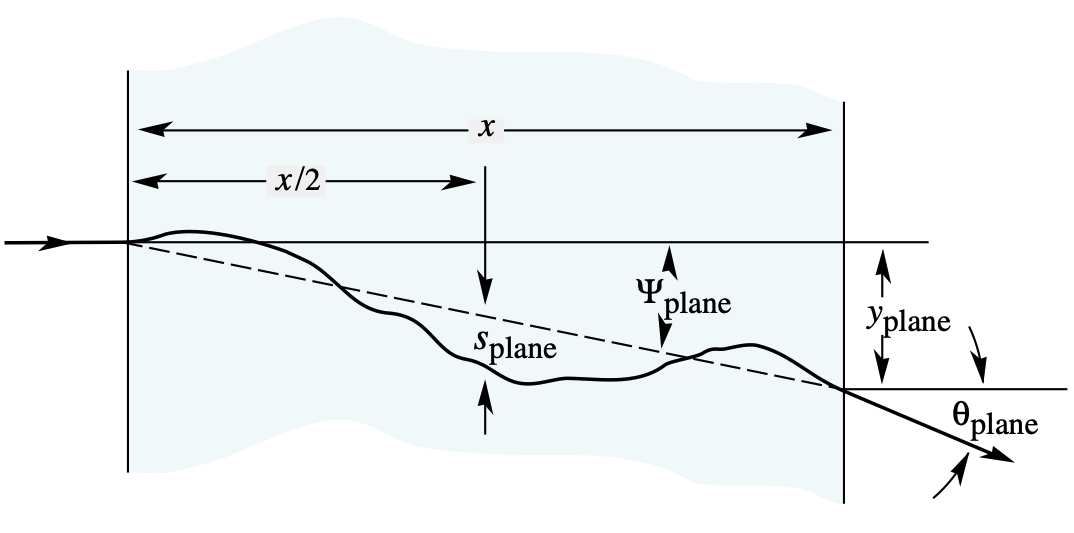
\includegraphics[width=0.65\linewidth]{figures/multi-scat.png}
    \caption{Schematic of the calculation of macroscopic mean deflection angle caused by multiple scattering~\cite{Zyla:2020zbs}.}
    \label{fig:multi-scat}
\end{figure}

The material effects described in this section, sections \ref{subsect:e-loss-heavy} and \ref{subsect:e-loss-electron}, are sufficient for Monte-Carlo simulations of the particle passage through material in the ITk. 
The overall trajectory can be discretized into small segments. 
The mean energy loss and Coulomb scattering angle over each segment can be estimated using equations \eqref{eq:6.1}, \eqref{eq:6.12}, \eqref{eq:6.15} and \eqref{eq:6.17}, along with the material distribution as shown in figure \ref{subfig:itk-rad-len}. The actual energy loss and scattering angle are then sampled from the corresponding distribution. 

\section{Simulated samples}
\label{sect:simulated-samples}
The development and evaluation of the new tracking algorithm in this thesis is carried out using a sample of simulated $pp\rightarrow t\bar{t}$ events at center-of-mass energy $\sqrt{s}=14$ TeV, with average pile-up ranging from 190 to 210.
The actual number of pile-up interactions in each event is randomly sampled from a Poisson distribution centred at the average pile-up. 
The hard-scattering event is generated using the \textsc{Powheg Box v2} \cite{Frixione:2002ik, Frixione:2007vw, Nason:2004rx, Alioli:2010xd} generator at next-to-leading order in QCD with the \textsc{NNPDF3.0nlo} \cite{Ball:2014uwa} Parton Distribution Functions (PDFs).
The $h_{\mathrm{damp}}$ parameter\footnote{ $h_{damp}$ is a resummation damping factor and one of the parameters that controls the matching of \textsc{Powheg} matrix elements to the parton shower and regulates the high-$p_T$ radiation against which the $t\bar{t}$ system recoils. } is fixed to $1.5m_{\mathrm{top}}$ \cite{ATL-PHYS-PUB-2016-020} and the top quark mass to $m_{\mathrm{top}} = 172.5$ GeV.
Parton shower and hadronization are modeled using \textsc{Pythia 8.230}\cite{Sjostrand:2014zea}, with the A14 set of tuned parameters \cite{ATL-PHYS-PUB-2014-021} and using the \textsc{NNPDF2.3lo} \cite{Ball:2012cx} set of PDFs.
A semi-leptonic final state, in which one of the two $W$-bosons descending from the top quarks decays to an electron or a muon, is enforced. 
The decay of bottom and charm hadrons are performed by \textsc{EvtGen 1.6.0}\cite{Lange:2001uf}.
The simulation described here follows the procedure detailed in reference~\cite{Aad_2025}.

To simulate the pile-up background, a large pool of soft minimum-bias interactions is generated. 
Each event is created by overlaying a number of min-bias sub-events on the hard-scattering sub-event, and then digitizing the detector response. 
A feature of MC simulation in ATLAS is that the pile-up sub-events are not uniquely generated for each events but randomly sampled from the common pool, resulting in a dataset whose events are guaranteed to feature different hard-scattering events, but may share a portion of their pile-up background. 
A dataset of 100000 $t\bar{t}$ events are simulated, from which a subset of 10000 events is identified to share no pile-up particles with the remaining 90000.
This subset is dedicated to machine learning training and performance evaluation.
The hard-scattering particles of the 90000 are used to train an algorithm to construct graphs from detector hits.


\chapter{The ATLAS track reconstruction chain}
\label{chap:atlas-reco-chain}

The High Luminosity era brings many challenges to event reconstruction in general and charged-particle tracking in particular, due to increased pile-up level and detector granularity. 
The current algorithm used in offline tracking scales super-linearly with pile-up and struggles to meet the future operational requirements. 
This motivates the development of an alternative algorithm that leverages modern hardware accelerators, such as the Graphic Processing Unit (GPU) or the Field-Programmable Gate Array (FPGA), to boost the reconstruction speed.
% The obvious questions arising when one proposes a new algorithm is: \textit{Does it perform the task as well as the existing algorithm?}, and \textit{if not, why?}. 
In this context, an understanding of the existing algorithm is necessary to adequately compare its performance to that of the proposed algorithm. 
% Answering such questions necessitates understanding of both the existing and the novel algorithms. 
This chapter describes the working principle of the Combinatorial Kalman Filter--the engine of charged-particle tracking, and the challenges facing it in the High-Lumnosity era.
The Kalman mechanism stems naturally from the least-square fit, which is also the basis of the discussion in chapter \ref{chap:tracking-performance}.

\section{Clusterization and space point formation}
\label{sect:cluster-spacepoint}

The first step of track reconstruction is the clusterization of the energy deposit on individual sensor cells recorded by the detector.
Figure \ref{fig:clustering} illustrates a particle passing through a planar pixel sensor and depositing a small amount of its energy. 
% the detector read-outs when a particle passes through a pixel module. 
Each sensor cell independently measures this energy and, when the energy exceeds a certain threshold, records a signal.
Throughout an event, a sensor may experience multiple passages of different particle trajectories, as shown on figure \ref{fig:sp-calcul}, so its collection of cell read-outs must then be sorted into groups of neighbouring cells likely to originate from the same particle. 
This process, called clusterization, transforms low-level information from individual sensor cells to a higher-level and more compact objects, called \textbf{clusters}. 

\begin{figure}[htb]
    \centering
        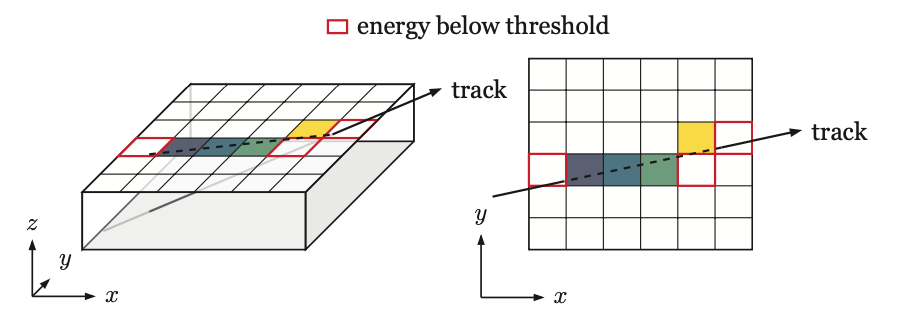
\includegraphics[width=0.8\textwidth]{figures/clustering.png}
    \caption{Formation of a pixel clusters from multiple cells. The particle deposits its energy in 7 cells, 5 of which receive charges exceeding the detection threshold and enter the clusterization \cite{paul-thesis}.}
    \label{fig:clustering}
\end{figure}

ATLAS traditionally uses a connected component analysis (CCA) \cite{CCA-pixel}, and more recently a neural network-based approach to clusterize cell read-outs\cite{clustering_nn}.
The intersection point $\mathbf{l}$ between the track and the sensor is estimated from the local coordinates $\mathbf{l}_i$ of each cells in the clusters
\beq
\label{eq:track-fit:1-1}
\mathbf{l} = \begin{cases}
    \frac{1}{N} \sum_i \mathbf{l}_i \\
    \frac{1}{\sum_i q_i} \sum_i q_i \mathbf{l}_i
\end{cases},
\eeq
where $q_i$ is the charge deposit on cell $i$. 
The first formula computes a simple vector mean of the cell location, and the second a charge-weighted mean. 
In the neural network approach, the cluster position and uncertainty are both predicted by the network and found to be more accurate than the (weighted) mean approach.

\begin{figure}[htb]
    \centering
        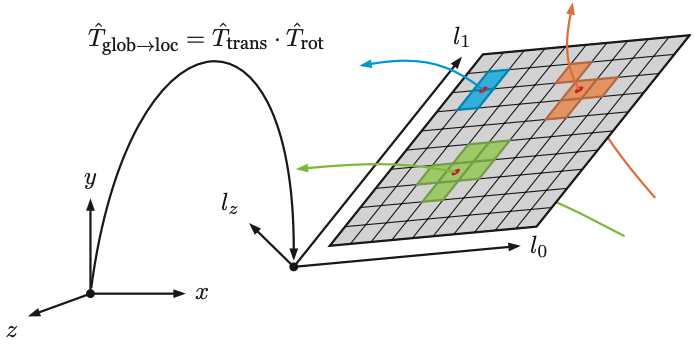
\includegraphics[width=0.8\textwidth]{figures/sp-calculation.png}
    \caption{The passage of a particle through a pixel sensor segmented in two dimensions. The energy deposit in each sensor cell is measured as a signal when it exceeds a measurement threshold. The true intersection point is estimated from the signal cells grouped together, called a cluster~\cite{paul-thesis}.}
    \label{fig:sp-calcul}
\end{figure}

A cluster can be regarded as a measurement made in the local coordinate of the measuring surface\footnote{For rest of this thesis, the terms ``measurement" and ``cluster" are interchangeable and refer to the same objects}.
From a cluster, the location of the hit in global coordinate, called the space point, can be derived.
Figure \ref{fig:sp-calcul} illustrates three particle tracks traversing a pixel sensor and inducing separate clusters. 
The true intersections are shown as red dots. 
An estimate of each of the true intersections between the trajectory and the sensor plane shown as red dots, is made in the clusterization step, and combined with the location and rotation of the sensor surface to obtain the space points.
In this sense, pixel space point formation is obtained from a change in reference frame of the cluster coordinates via a series of translational and rotational transformations. 

\begin{figure}[htb]
    \centering
    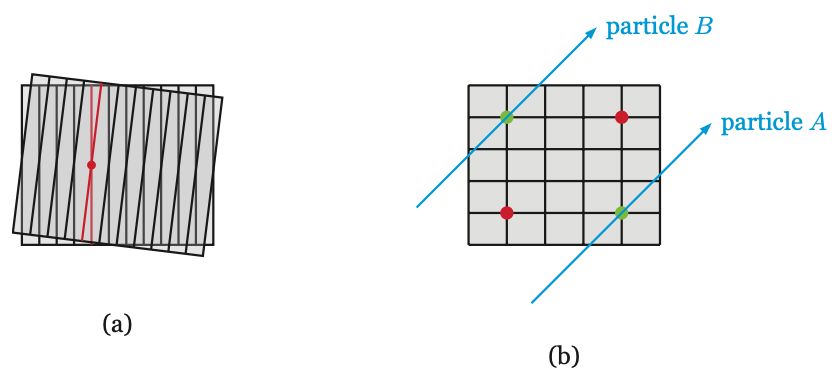
\includegraphics[width=0.8\linewidth]{figures/sp-calcul-strip.png}
    \caption{A pair of strip sensors are used to reconstruct a 3-dimensional estimate of the particle's true impact point (a). Ambiguity arises when more than one particle hit a strip module, leading to more combinations than particles (b) \cite{paul-thesis}. }
    \label{fig:sp-calcul-strip}
\end{figure}

While there is a one-to-one correspondence between a pixel cluster and a pixel space point, the space point formation in the strip detector is more complicated.
Strip modules are finely segmented in only one direction, rendering each measurement one-dimensional, in contrast to the two-dimensional measurements on a pixel module.
To obtain a three-dimensional position estimate, two strip clusters from the same layer are combined, as shown in fig. \ref{fig:sp-calcul-strip}. 
The local position of the hit along the thinly segmented dimension is established with high resolution.
Thanks to the stereo angle between the modules, an estimate of the second coordinate is made from the intersection of the strip cells, albeit with lower resolution. 
These measurements are then transformed to a global position estimate, as described above. 

% Ambiguity arises when multiple particles hit the same pair of strip modules, each generating two clusters, as shown on the left figure of \ref{fig:sp-calcul-strip}. 
% As the number of cluster combinations exceeds the number of particles, ghost space points are created by false association of clusters. 

In the current track reconstruction chain, space points are used to build track seeds, which are small groups of hits likely to originate from the same particle. 
A dedicated seeding stage create large number of seeds each containing three space points, which are subsequently fed to a track building algorithm. 
The latter extends the seed by iteratively adding clusters that are compatible with the corresponding track state.
A small number of clusters in the final track candidate come from the seed space points, and the rest from individually incorporated clusters on the track path.

Finally, we note an important consequence of the 2-cluster composition of the strip space point.
Despite meticulous optimization of the detector layout, a particle does not always leave two hits on a strip layer. 
Silicon sensors have inherent inefficiency, which means that a particle may traverse a detector module without inducing a signal.
This phenomenon occurs in both sub-detectors of the ITk, but is very unlikely.
More importantly, in the strip detector, a particle may approach a layer in a direction such that it intersects only one of two physical strip modules (see section \ref{sect:itk-overview} for a description of the strip detector). 
For any reason, when a strip layer records a \textit{lone} cluster, it is ignored by the space point formation algorithm, resulting in a cluster inefficiency amongst the space points.
This inefficiency is of limited consequence in the current ATLAS reconstruction chain, because space points are only used for track seeding.
However, an algorithm that builds tracks from space points would not see lone clusters in the input, which may cause potential impacts on its performance.
This issue will become important for the new algorithm and be described in chapter \ref{chap:tracking-performance}.

\section{The least-square fit}
\label{sect:track-fit}

A track candidate is a set of measurements made by sensitive detector elements on the particle's trajectory. 
The latter is mathematically represented by a set of parameters describing its position and momentum as it traverses the detector. 
Although in idealized situations, the track may be parametrized by constants of motion, in a realistic detector, even these constants vary over time, due to random material effects. 
Therefore, a necessary ingredient to describe the trajectory is the solution to the equation of motion given the detector setup. 
From an initial value and the precise magnetic field on a dense grid of sampling points, the equation of motion is numerically integrated to obtain the a description of that particle state as it evolves along the trajectory. 

Let $\bfx\in \mathbb{R}^d$ represent the state of the particle and vary as a function of the arc length $s$ along the trajectory\footnote{Since $s=vt$, this is equivalent to parametrization in time.}, so that 
\beq
\label{eq:track-fit:1}
\bfx = \bfx(s)
\eeq
We will keep the discussion here general and note that any set of parameters from which the instantaneous position and momentum of the particle can be derived is usable. 
The choice of parametrization in ATLAS is discussed in section \ref{sect:chi2-fit}.
In general, track parameters can be regarded as the internal state of the particle, which is not directly measurable.
Instead the measurements are made at discrete points on the trajectory where a sensitive module is present.
Each measurement $\bfm_i$ can then be modelled as a deterministic function of the track state at that the measuring surface $\bfx_i$ superimposed by a random experimental noise $\epsilon_i$.
\beq
\label{eq:track-fit:2}
\bfm_i = h_i(\bfx_i) + \epsilon_i.
\eeq
The function $h_i:\mathbb{R}^d \rightarrow \mathbb{R}^n$, called the \textit{measurement model}, projects the $d$-dimensional state vector $\bfx_i$ on the $i$-th surface to an $n$-dimensional measurement vector. 
Its functional form depends on the type of measuring surface, hence the subscript.
For example, a measurement on a pixel module is intrinsically different from one on a strip module\footnote{A pixel cluster is a $2D$ measurement, while a strip cluster is $1D$.}, so their measurement models naturally differ. 

The experimental noise $\epsilon_i$ also depends on the type of measuring surface. 
However, it is generally assumed to be unbiased with finite variance, namely
\beq
\label{eq:track-fit:3}
E[\epsilon_i] = \mathbf{0}, \quad 0<\sigma(\epsilon_i^{(j)}) < +\infty ,\forall \, j \in [n],
\eeq
where the superscript denotes the $j$-th component of the $n$-dimensional error vector.
The covariance matrix of $\epsilon$ is an important ingredient of the least-square fit, denoted by
\beq
\label{eq:track-fit:4}
\mathbf{V}_i = E[\epsilon_i \epsilon_i ^T]
\eeq

As mentioned above, the state vector evolves along the trajectory, governed by the Equation of Motion (EOM), the solution to which is called the track model. 
The system evolution can be written as a recursive process
\beq
\label{eq:track-fit:5}
\bfx_i = \bfx(s_i) = f_{i-1} (\bfx_{i-1}).
\eeq
The extrapolation function $f_{i-1}: \mathbb{R}^d\rightarrow\mathbb{R}^d$ projects the track state from the previous measuring surface $\bfx_{i-1}$ to the current surface. 
Its functional form depends on the equation of motion, which in turns depends on detector characteristics, such as its magnetic field and layouts.
As the EOM is in general a second-order non-linear differential equation, a close-form solution, if it exists, is likely non-linear.
However, in practice, the EOM is often linearized and numerically integrated by, for example, Euler's method, allowing a linear, albeit recursive and potentially expensive solution
\beq
\label{eq:track-fit:6}
\bfx(s_{i-1} + \Delta s)\approx \bfx(s_{i-1}) +     \frac{\partial \bfx'}{ds'} \Big \vert _{s'=s_{i-1} }\Delta s + \mathcal{O}((\Delta s)^2),
\eeq
where the derivative is calculated from the dynamical equation of the system. 
More sophisticated numerical methods can be used, but in principle, it is possible to approximate the transport equation \eqref{eq:track-fit:5} as a linear recursive relation. 
The benefit of such linearization is that we can write the track state on any surface $\bfx_i $ as a simple linear function of some initial value on a reference surface $\bfx_0$,
\beq
\label{eq:track-fit:7}
\bfx_i = f_{i-1}(x_{i-1}) = f_{i-1}(f_{i-2}(\bfx_{i-2})) = f_{i-1} \circ f_{i-2} \circ \dotsc \circ f_0 (\bfx_0) = f_i (\bfx_0),
\eeq
and take $\bfx_0$ as \textit{the} estimated track parameters.

Track fitting is now reduced to finding an estimator $F$ from the set of measurements $M=\{\bfm_1,\dotsc,\bfm_N\}$ to the parameter space, such that (1) the estimate $\hat{\bfx}_0=F(M)$ is unbiased
\beq
\label{eq:track-fit:8}
E[\hat{\bfx}_0] = \bfx_0
\eeq
and (2) of minimum variance
\beq
\label{eq:track-fit:9}
E[(F(M) - \bfx_0)^2] = \min_{F'} E[(F'(M) - \bfx_0)^2]
\eeq
The Gauss-Markov theorem \cite{gauss-markov} states that among the class of linear and unbiased estimators, the Least Squares Estimator (LSE) has minimum variance, provided a linear track model, purely statistical\footnote{i.e. independent of $\bfx$}, unbiased and uncorrelated errors $\epsilon_i$. 
The LSE is obtained by minimizing the $\chi^2$-function, defined as
\beq
\label{eq:track-fit:10}
\chi^2 = \sum_{i=1}^N [\bfm_i - h_i(f_i(\bfx_0))]^T \mathbf{V}_i^{-1}[\bfm_i - h_i(f_i(\bfx_0))],
\eeq
where both $h_i$ and $f_i$ are now assumed to be linear.
The linearity of $h_i$ can be achieved by a careful choice of parametrization, such as the one used by ATLAS, discussed in section \ref{sect:chi2-fit}.
The estimator is simply the solution to
\beq
\label{eq:track-fit:11}
\nabla  \chi^2(\bfx_0) = 0
\eeq

\section{Iterative track fit}
\label{sect:kalman-filter}

Because the LSM considers all measurements at the same time, it is a global fitting method. 
It can be shown that in situations where the material effects described in section \ref{sect:material-effects} cannot be ignored, the minimization of the $\chi^2$-function translates to the inversion of a non-diagonal covariance matrix whose dimension grows with the number of measurements $N$. 
This computation can become a significant bottleneck in complex and granular detectors (see chapter 3 of reference \cite{Regler2000-ie} for more details).

The Kalman formalism \cite{Mankel_2004, BILLOIR1984352, FRUHWIRTH1987444} offers a faster alternative to global fit that, crucially, yields optimal estimates for Gaussian measurement uncertainties. 
The track state still evolves as a linear dynamical system.
Multiple scattering and energy loss due to material interactions are modelled as random process noise $\mathbf{w}$ added to the transport equation 
\beq
\label{eq:track-fit:12}
\bfx_i = \mathbf{F}_{i-1}\bfx_{i-1} + \mathbf{w}_{i-1},
\eeq
where the matrix $\mathbf{F}_{i-1}$ is the track model given in equation \eqref{eq:track-fit:5} now written in the explicitly linear form. 
The process noise $\mathbf{w}$ has a covariance denoted by
\beq
\label{eq:track-fit:13}
\mathbf{Q} = E[(\mathbf{w} - E[\mathbf{w}])(\mathbf{w} - E[\mathbf{w}])^T]
\eeq
Instead of minimizing a $\chi^2$-function over all measurements, the Kalman procedure iteratively incorporates measurements into an existing estimate of the track parameters. 
Each iteration inverts a single $n\times n$ matrix, so in total, $N$ inversions of $n\times n$-matrices are needed, where $n$ is the number of measurement coordinates\footnote{In typical ATLAS parametrization, $n=2$} and $N$ the number of measurements, as opposed to inverting an $(nN)\times (nN)$ matrix in the LSM.
The information from the measurement is used to constrain the estimate and reduce the error. 
The procedure is carried out in the following 3-step recipe. \\
\textbf{Step 1: Prediction}. Suppose the measurement $\bfm_i\in M$ is being incorporated. 
Let $\bfx_{i-1}$ and $x_{i}^{i-1}$ denote the track state before the inclusion of $\bfm_i$, and its projection to the measuring surface of $\bfm_i$ by the transport equation.
In addition, denote the covariance of the estimate as $\mathbf{C}$,
\beq
\label{eq:track-fit:13-1}
\mathbf{C} = E[(\bfx - E[\bfx])(\bfx - E[\bfx])^T],
\eeq
so that the covariance before inclusion is $\mathbf{C}_{i-1}$.
\textit{Neither} of $\bfx_{i-1}$ nor $\bfx_i^{i-1}$ contains information from $\bfm_i$, nor any material effect during the propagation, 
\beq
\label{eq:track-fit:14}
\bfx_i^{i-1} = \mathbf{F}_{i-1}\bfx_{i-1}.
\eeq
The stochastic noise due multiple Coulomb scattering and energy loss corrections is instead superimposed on the projected covariance,
\beq
\label{eq:track-fit:16}
\mathbf{C}_i^{i-1} = \mathbf{F}_{i-1}\mathbf{C}_{i-1}\mathbf{F}_{i-1}^T + \mathbf{Q}_{i-1}.
\eeq
\textbf{Step 2: Filtering}. The predicted track state in \eqref{eq:track-fit:14} is combined with the present measurement $\bfm_i$ to yield the updated estimate $\bfx_i$ 
\beq
\label{eq:track-fit:17}
\bfx_i = \bfx_i^{i-1} + \mathbf{K}_i(\bfm_i - \mathbf{H}_i\bfx_i^{i-1}).
\eeq
$\mathbf{K}_i$ is called the Kalman gain matrix 
\beq
\label{eq:track-fit:18}
\mathbf{K}_i = \mathbf{C}_i^{i-1}\mathbf{H}_i^T(\mathbf{V}_i + \mathbf{H}_i\mathbf{C}_i^{i-1}\mathbf{H}_i^T)^{-1}.
\eeq
Intuitively, $(\bfm_i - \mathbf{H}_i\bfx_i^{i-1})$ represents the difference between the actual measurement and the expected measurement given the predicted track state.
If the measurement exactly equals its predicted value, it supports the predicted track state, so the update track state equals its predicted value.
No new information is added to the filtered estimate in such a case.
Therefore, we can think of the Kalman matrix as the information gained from any disagreement between the predicted and the actual measurement, hence its denomination. 

The covariance of the estimate is updated from its prediction as
\beq
\label{eq:track-fit:19}
\mathbf{C}_i = (\mathbf{I} - \mathbf{K}_i\mathbf{H}_i)\mathbf{C}_i^{i-1}.
\eeq
The uncertainty from stochastic noise and the measurement uncertainty are respectively encoded in $\mathbf{C}_i^{i-1}$ and $\mathbf{K}_i$. 
Both sources of uncertainty thus contribute to the filtered covariance, as expected.
Both the state vector and its covariance are updated by incorporating a new measurement and the material effects from propagating the particle from its last known position.

Repeated applications of prediction and filtering incorporate all measurements to refine the track state from its initial value $\bfx_0$ \\
\textbf{3. Smoothing}. The prediction and filtering sequence refines the track state in the forward direction.
This means that an estimate at the end of the trajectory is better than one at the beginning. 
It is, however, desirable that all estimates receive information from all measurements, rather than those preceding them. 
The smoothing step achieves this goal by working backward from the outermost measurement and updating a state vector at step $i$ using the state vector at step $i+1$
\beq
\label{eq:track-fit:20}
\bfx_i^N = \bfx_i + \mathbf{A}_i(\bfx_{i+1}^N - \bfx_{i+1}^i),
\eeq
in which the superscript $N$ signifies an estimate incorporating all $N$ measurements. 
$\mathbf{A}_i$ is called the smoothing gain matrix, defined as
\beq
\label{eq:track-fit:21}
\mathbf{A}_i = \mathbf{C}_i \mathbf{F}_i^T(\mathbf{C}_{i+1}^i)^{-1}.
\eeq
Only after filtering through all measurements on track can the smoothing be effected. 
In ATLAS terminology, the former is therefore referred to as the forward filter, while the latter backward smoothing.
The initial track state $\bfx_0$, or the state on any other surface, real or imaginary, can be refined or extrapolated using the entire measurement set. 

% [Discuss the connection to the minimum variance principle here, and mention the global chi2 under the hood]

\section{Combinatorial Kalman Filter}
\label{sect:CKF}
Thanks to its iterative mechanism, the Kalman formalism can be extended from track fitting to track finding, called the Combinatorial Kalman Filter (CKF). 
From a track seed containing $k$ measurements, it estimates the initial value $\bfx_k$ and projects it to the next surface using equation \eqref{eq:track-fit:12}.
In the filtering stage, instead of incorporating a given measurement, as in the case of track fitting, it considers all measurements on the target surface falling into a search window defined by the projected measurement covariance.
By filtering each candidate measurement $l$, it computes a filtered track state and measurement residual
\beq
\label{eq:track-fit:22}
\mathbf{r}_{k+1, l} = \bfm_{k+1, l} - \mathbf{H}_{k+1}\bfx_{k+1, l}.
\eeq
The increment in $\chi^2$ is computed from the residual
\beq
\label{eq:track-fit:23}
\chi^2_{+, l} = \mathbf{r}_{k+1, l}^T[(\mathbf{I} - \mathbf{H}_{k+1}\mathbf{K}_{k+1}) \mathbf{V}_{k+1, l}]^{-1} \mathbf{r}_{k+1, l}.
\eeq
All candidate measurements $l$ whose contribution to the global $\chi^2$ falls before a certain threshold are admitted, creating the same number of branches from the track seeds.
The procedure is repeated till no more measurements can be incorporated. 
The output from a given track seed is usually a large set of track candidates each originating from a combination of branching connections, hence the \textit{combinatorial} denomination.

The track candidate is characterized by a global $\chi^2$ equal to the sum of the contributions from individual measurements in equation \eqref{eq:track-fit:23}.
Several candidates might be ruled out based on the mean $\chi^2_{track} / \abs{M_{track}}$, as well as other quality cuts. 
To guarantee tracking efficiency, a large number of track seeds are produced and considered by the CKF.
The number of considered track seeds combined with the number of combinations per seed results in significant track redundancy and overlapping measurements. 
An ambiguity resolution step globally sorts through the track candidates and assigns each measurement to mostly a unique track, effectively reducing them to a set of tracks of highest quality and compatibility to real particles. 

\section{Computational cost of track reconstruction}
\label{sect:computational-cost-ckf}

Inner tracking is one of the most expensive tasks of event reconstruction. 
For instance, table \ref{tab:reco-time-breakdown} illustrates the CPU consumption in \hssec~of each reconstruction stage under Run 2 conditions but scaled to $\expval{\mu}=90$ \cite{CERN-LHCC-2020-015}.
Track reconstruction dominates the computing budget, consuming $67\%$ of the total reconstruction time.
This contribution will only get worse at pile-up 200, due to the strong scaling behaviour of the Combinatorial Kalman Filter and the Ambiguity Resolution step which necessarily follows.

\begin{table}[h!]
    \centering
    \begin{tabular}{|c|c||c|c|c|c||c|}
    \hline
       Detector  & $\expval{\mu}$ & Tracking & Calo and M.S & Combined Reco. & Monitoring &  Total \\
       \hline
        Run 2 & 90 & 1137 & 149 & 301 & 106 & 1693 \\ \hline
    \end{tabular}
    \caption{The CPU required in \hssec~to reconstruct a Run 2 data event using the corresponding software release at average pile-up 90 using. The total reconstruction time is broken down into inner tracking, Calorimeter and Muon Spectrometer reconstruction, and Monitoring. Numerical figures taken from reference \cite{CERN-LHCC-2020-015}.}
    \label{tab:reco-time-breakdown}
\end{table}

Within Inner Tracking, the tracking finding step described in this chapter consumes the largest CPU resource. 
Listed in table \ref{tab:tracking-time-breakdown} are the cost of each step in the tracking stage, assuming the pile-up levels of 140 and 200. 
In the default tracking chain, the tracking finding and ambiguity resolution steps dominate the total CPU consumption. 
Although listed as separate items, the former's performance is severely degraded without the latter, so they should be considered together as one item, which occupies $83\%$ of the overall computing consumption for inner tracking at pile-up 200.

\begin{table}[h!]
    \centering
    \begin{tabular}{|c|c||c|c|c|c|c||c|}
    \hline
       $\expval{\mu}$  & Algorithm & Decoding & Clustering & S.P. Formation & CKF & Am. Reso. &  Total \\
       \hline \hline
        140 & Default & 1.2 & 17.1 & 6.0 & 41.1 & 58.2 & 124 \\ \hline
        140 & Fast & 1.2 & 4.5 & 0.9 & 12.4 &  & 19.0 \\ \hline \hline

        200 & Default & 1.6 & 26.3 & 8.6 & 85.8 & 92.0 & 214 \\ \hline
        200 & Fast & 1.6 & 6.3 & 1.2 & 22.6 & & 31.7 \\ \hline
    \end{tabular}
    \caption{The CPU required in \hssec~to reconstruct a $t\bar{t}$ MC event with $\expval{\mu}=140$ and 200 in the ITk. The total track reconstruction time, evaluated for both the default and an optimized CKF-based chains, is broken down into individual steps, most significant of which are clustering, space point formation, CKF-based track finding and ambiguity resolution. An Intel Xeon E5-2620v2 processor with 2.1 GHz and six physical cores per CPU was used. The CPU time is multiplied by an HS06 factor of 17.8 for single-thread running. Numerical figures taken from reference \cite{ATL-PHYS-PUB-2019-041}.}
    \label{tab:tracking-time-breakdown}
\end{table}

ATLAS has carried out major optimizations of the default CKF chain to improve its CPU performance, shown in table \ref{tab:tracking-time-breakdown} as Fast tracking. 
Track seeds used to initialize the CKF are created exclusively from pixel space points, enabled by the increased number of expected pixel hits thanks to an additional layer and the full $\eta$-coverage of the ITk compared to the ID. 
A tighter track selection and precise cluster calibrations are used to remove duplicate and fake tracks after the track finding step, in lieu of the costly ambiguity resolution step. 
These changes, along with other incremental improvements, allows running the track reconstruction pass approximately 8 times faster than the default chain, as illustrated in table \ref{tab:tracking-time-breakdown}, but with a loss in physics performance, as shown in figure \ref{fig:fast-default-phys} \cite{ATL-PHYS-PUB-2019-041}.
Despite the impressive acceleration, the fast track chain still is far from ready for production due to both latency and tracking performance.

\begin{figure}[t]
    \centering
    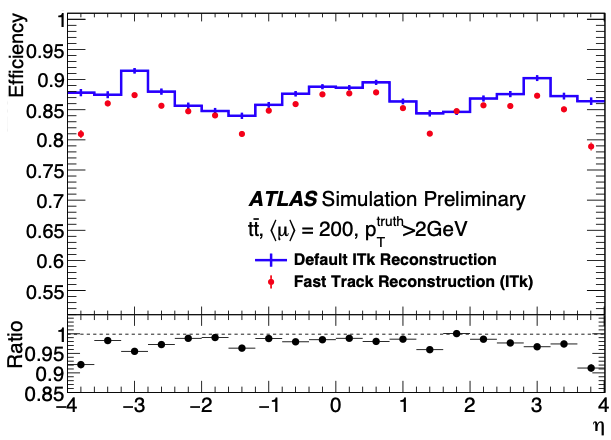
\includegraphics[width=0.49\textwidth]{figures/eff-fast-def.png}
    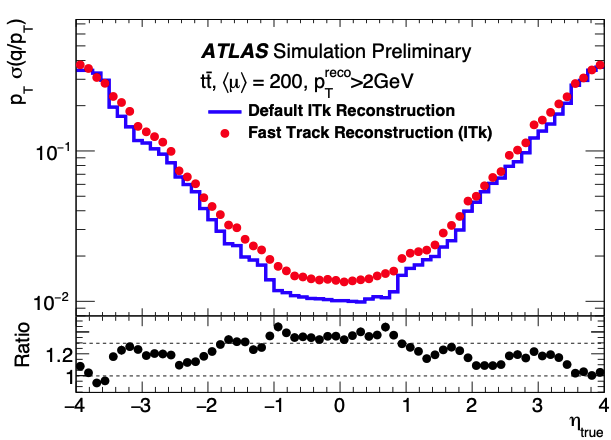
\includegraphics[width=0.49\textwidth]{figures/res-fast-def.png}
    \caption{Tracking efficiency (left) and track parameter resolution (right) as functions of the truth particle's pseudorapidity, evaluated at $\expval{\mu}=200$. The bottom plots show the ratio of the corresponding metric observed in the fast chain to that in the default chain~\cite{ATL-PHYS-PUB-2019-041}.}
    \label{fig:fast-default-phys}
\end{figure}

Along with optimizing the traditional event reconstruction algorithm, ATLAS is actively pursuing significant modernization of its analysis software, both online and offline. 
As outlined in reference \cite{CERN-LHCC-2022-005}, the primary challenge of the HL-LHC era will be the effective use of General Purpose Graphics Processing Units (GP-GPUs), which are becoming ubiquitous in large High-Performance Computing (HPC) facilities and data centers.  
They can accelerate suitable applications by orders of magnitude, many of which have already been deployed in ATLAS. 
Examples include Fast Simulation \cite{atlfast}, Particle Flow \cite{particle-flow}, and $b$-tagging graph neural networks \cite{GN1}.
Exploiting this computing resource requires recasting current software on the hardware accelerators, for instance the \hyperlink{https://github.com/acts-project/traccc}{\textsc{TrackCC}} project~\cite{andreas_salzburger_2025_15260074}, or designing new algorithms inherently compatible with them.
In addition, because of the increased track multiplicity in HL-LHC, online applications such as trigger and data acquisition will likely be migrated to accelerators, and thus, new hardware-accelerated algorithms are further incentivized for offline software to maintain synergies between the two computing domains.
In this context, the next big component in event reconstruction to be modernized is inner tracking, attracting substantial interest and investment in person power within ATLAS.
The work done in this thesis plays a significant role in this effort, resulting in a competitive candidate for an end-to-end, machine learning-based and fully GPU-compatible algorithm for track reconstruction. 
The remaining chapters of this thesis describe its development and latest results.

% For example, in a homogeneous magnetic field and no material interaction, the track model is a helical orbit with radius $R_{H}=\frac{p_T}{kqB}$ specified by an initial position $\mathbf{r}_0$ and momentum $\mathbf{p}_0$. 
% The magnetic field in ATLAS is far too complex for such an analytical solution to exist. In addition, interactions with detector material deviate the trajectory further from a perfect helix, and, as a result, the track model must be obtained from numerical integrations. 


% \section{Ambiguity Resolution}

% \section{The cost of tracking}

% \section{Summary}
% \chapter{An new tracking approach}



\chapter{Track reconstruction with Graph Neural Networks}
\label{chap:graph-construction}

% The Combinatorial Kalman Filter (CKF) builds a track candidate locally, by incorporating clusters in the next layer which are compatible to an existing track state. 

Graph Neural Networks (GNNs) were first proposed in 2018 as an alternative track finder to the Combinatorial Kalman Filter (CKF)~\cite{farrell2018noveldeeplearningmethods}.
Developed and tested on the \textsc{TrackML} dataset \cite{trackml-particle-identification}, they demonstrated excellent physics performance and favourable scaling behaviour~\cite{exatrkx, choma2020trackseedinglabellingembeddedspace}.
Fundamentally, GNN-based algorithms represent a shift from the local track finding approach of the CKF to a global approach.
Instead of extending a track seed with compatible hits in sequence, as described in chapter \ref{chap:atlas-reco-chain}, 
global track finding considers simultaneously a set of connections between detector hits and finds those that are most likely to belong to true particle tracks.
This set should contain most of the true connections and can be quite large, but the ability to parallelize the computation on GPUs makes this approach an attractive 
alternative to the sequential mechanism and redundancy of the CKF.
% No longer is a need to loop through a set of redundant track seeds, which makes the CKF slow and requires a costly ambiguity resolution.
% The GNN ``looks at" all possible candidate tracks in an event at the same time, significantly accelerating the recognition of track patterns thanks to GPU-powered parallelization.
The shift from hit finding to connection finding necessitates a change in representation of the collision event from a point cloud to a collection of nodes and edges, the very definition of a \textbf{graph}. 
This approach therefore relies on graph data structure.

The work documented in this thesis builds upon that of reference \cite{exatrkx}, which examined the physics and computing performance 
of the GNN on the TrackML dataset~\cite{trackml-particle-identification}, and of reference \cite{Caillou:ATL-ITK-PROC-2022-006}, 
which made initial strides in applying the GNN to data from full detector simulation using ITk geometry. 
It contributes numerous developments that bring the new approach closer to the state-of-the-art performance.
Neural network architectures undergo significant refinements.
The algorithm is fully integrated into the official ATLAS software framework~\cite{atlas_collaboration_2021_4772550}, thus enabling direct performance comparison to the CKF.
Finally, many components are computationally optimized, resulting in competitive reconstruction speed.
This chapter commences the discussion with an overview of the algorithm and the construction of graphs from detector data. 
Subsequent stages of the algorithm, especially the graph neural network, are detailed in chapters \ref{chap:gnn} and \ref{chap:track-building}, and finally the results are presented in chapters \ref{chap:tracking-performance} and \ref{chap:computing-performace}.
% In the previous chapter, we propose a global approach to the problem of track finding in the ITk as an alternative to the existing local approach of the Combinatorial Kalman Filter. 


\section{Overview}

The GNN-based approach, illustrated in figure \ref{fig:gnn4itk} and hereafter referred to as the \textbf{GNN4ITk} algorithm, creates track candidates by segmenting a graph constructed from the collection of space points in each event. 
A graph $G(V,E)$ is a mathematical structure consisting of a set of nodes $V$, and a set of pairwise connections $E$ between these nodes. 
Each node $v_i \in V$ represents a space point, and an edge $e_{ij} \in E$ a hypothesis that the space points represented by $v_i$ and $v_j$ are created from successive energy deposits by the same particle. 
In addition, a ground truth graph $G_{truth}= (V, E_{truth})$ is defined from the same set $V$ and the connections between successive space points on the trajectories of all particles in the event, denoted by $E_{truth}$, oriented in the direction of increasing distance from the particle's production vertex. 
An edge $e_{ij}\in E$ is true if it is also in the truth graph, i.e. 
\begin{equation}
\label{eq:9.1}
y_{ij} = 1_{[e_{ij} \in E_{truth}]},
\end{equation}
and fake otherwise. 
A graph neural network is used to assign to every edge $e_{ij} $ a score $s_{ij} = P[y_{ij} = 1]$, representing a continuous function of the probability that the edge in question is true.
To obtain the probability, a calibration step is sometimes needed \cite{Feng_2022}. 
For our purpose, a score threshold is selected to satisfy certain requirements on the edge efficiency evaluated on the validation set.
Edges with scores under the threshold are eliminated, and the remaining graph is segmented into \textbf{track candidates}, collections of nodes believed to originate from the same particle.

\begin{figure}[h!]
    \centering
    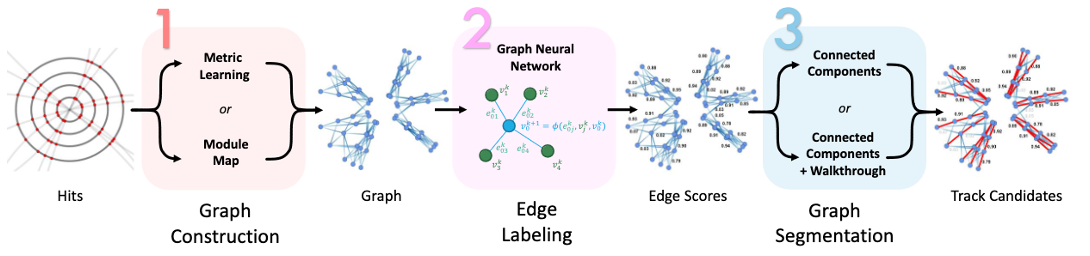
\includegraphics[width=\textwidth]{figures/gnn4itk.png}
    \caption{The GNN4ITk algorithm consists of three distinct stages. The first stage constructs a graph from the set of space points in an event, each acting as a node. The second stage identifies edges connecting consecutive nodes on a particle tracks from other edges. The last stage construct track candidates by segmenting the graph using the output of the second stage. The algorithm's output consists of individual track candidates each as a set of space points believed to belong to the same particle.}
    \label{fig:gnn4itk}
\end{figure}

\section{Target, non-target particles and evaluation metrics}
\label{sect:eval-metrics}
At $\epu=200$, each collision event produces $\expval{N}\approx 10000$ final-state stable particles, the majority of which are of little interest to the physics program in ATLAS. 
They include, for example, low-momentum particles from background processes or particles which leave too few hits to be considered reconstructible.
The remaining particles can be broadly categorized by the interaction from which they emerge. 
Primary particles are produced in the luminous area directly from proton-proton interactions. 
Only particles that are stable enough to traverse the detector, including protons, electrons, muons, pions, etc can be reconstructed.
Secondary particles arise from the interaction of stable primary particles with detector material, such as $\delta$-ray electrons and nuclear interaction products. 
The CKF chain does not target secondary particles for reconstruction, due to the high computational cost to simultaneously consider them.
In the same spirit, throughout the GNN4ITk chain, we identify these particles prior to model training and exclude them from the loss function, as well as performance evaluation.

Since a secondary interaction occurs when the primary particle has travelled a distance from the luminous region, their vertices are often considerably further from the origin than the primary counterpart. 
Shown on figure \ref{fig:vertex-spectrum}, the majority of primary vertex positions are located at $v_r < 2$ cm and $v_z < 20$ cm, in contrast to secondary vertices, whose distributions of $v_r$ and $v_z$ are more spread-out and with longer tails.
% for secondary particles than their primary counterpart, which terminates at $v_r<10$ cm and $\abs{v_z}< 20$ cm, see figure \ref{subfig:radius-spectrum}.
This distinction allows us to select primary particles in training by requiring the production vertex to be within 26 cm from the origin.
As we will see in chapter \ref{chap:tracking-performance}, the ATLAS reconstruction chain eliminates secondary particle tracks by applying selection cuts on the impact parameters, which are good estimates of the vertex point, of $\abs{z_0}\le 20$ cm and $\abs{d_0}\le10$ cm. 

\begin{figure}[h!]
\begin{subfigure}[b]{0.49\textwidth}
    \centering
    \includegraphics[width=\textwidth]{figures/vr-hist.png}
    \caption{}
    \label{subfig:radius-spectrum}
\end{subfigure}
\begin{subfigure}[b]{0.49\textwidth}
    \centering
    \includegraphics[width=\textwidth]{figures/vz-hist.png}
    \caption{}
    \label{subfig:z-spectrum}
\end{subfigure}
    \caption{Distributions of the production vertex position on the transverse plane (a) and along the $z$-axis (b) of simulated particles in $t\bar{t}$-events at $\epu=200$ for non-primary and primary particles. Primary vertices are restricted to a small region around the interaction point, whereas non-primary vertices can occur throughout the detector.}
    \label{fig:vertex-spectrum}
\end{figure}

As we have seen in section \ref{subsect:e-loss-electron}, electrons and positrons uniquely undergo significant energy loss due to Bremsstrahlung, and often follow trajectories that deviate from a helix. 
To guarantee good electron efficiency without compromising that of other particles, the ATLAS chain reconstructs electron tracks in a separate pass with a specialized parameter estimation technique. 
Similarly, we avoid training models on ``irregular" electron tracks by excluding their contribution from the loss function.

Because each simulated event is generated from one hard-scattering (HS) collision and on average 200 pile-up collisions (section \ref{sect:simulated-samples}), particles originating from soft interactions outnumber HS particles by about two orders of magnitude, (figure \ref{subfig:eta-spectrum}). 
HS particles are generally more energetic; their $\pT$ spectrum stretches up to 100 GeV, whereas that of pile-up particles strongly peaks at $\pT<1$ GeV and terminates at 20 GeV, as shown in figure \ref{subfig:pt-spectrum}. 
% widely differ, with the former having a much longer tail.
As a consequence, a loss function calculated from all edges in the event is dominated by examples from low-$\pT$ tracks and bias the model at the expense of high-$\pT$ HS particles that represent the interesting physics.
This data imbalance largely impacts the performance, since in the presence of the magnetic field, low-$\pT$ particles have larger curvature and therefore different track pattern than do high-$\pT$ particles.
In addition, the CKF chain also targets high-\pT particle in the primary pass.
Therefore, we neglect the contribution to the loss function from particles of $\pT<1$ GeV.

\begin{figure}[h!]
\begin{subfigure}[b]{0.49\textwidth}
    \centering
    \includegraphics[width=\textwidth]{figures/pt-hist.png}
    \caption{}
    \label{subfig:pt-spectrum}
\end{subfigure}
\begin{subfigure}[b]{0.49\textwidth}
    \centering
    \includegraphics[width=\textwidth]{figures/eta-hist.png}
    \caption{}
    \label{subfig:eta-spectrum}
\end{subfigure}
    \caption{Distributions of transverse momentum \pT (a) and pseudorapidity (b) of simulated particles in $t\bar{t}$-events at $\epu=200$ separated according into hard-scattering and pile-up particles. Soft pile-up particles have low \pT, whereas hard-scattering particles have a wider \pT distribution. The former is two orders of magnitude more abundant than the latter.}
    \label{fig:pt-eta-spectrum}
\end{figure}

In light of this discussion, we sort truth particles into two subsets by the following criteria
\begin{enumerate}
    \item \textbf{Target} particles: primary particles from both hard-scattering and pile-up interactions, which have $\pT>1$ GeV and $\abs{\eta}<4$, leave at least 3 hits in the tracker, are produced at a transverse radius $R<26$ cm, and are not electron nor positrons.
    \item \textbf{Non-target} particles: The rest of truth particles, including electrons and other particles not satisfying the kinematic selection.
\end{enumerate}
In the same manner, the subset of $E_{truth}$ comprising exclusively connections from target particles is called the target truth edges and denoted as $E_{truth,target}$. 
A subset of non-target truth edges is defined as $E_{truth, non-target} = E_{truth} - E_{truth,target}$. 
The objective of global track finding then is to identify as many target truth edges and to misidentify as few fake edges as possible.
Two metrics are defined from the edge sets to quantify these criteria.
The first is the \textbf{edge efficiency} $\epsilon$: the fraction of target true edges present in a given edge set $E$
\begin{equation}
\label{eq:9.2}
\epsilon = \frac{\abs{E \cap E_{truth,target}  }} {\abs{E_{truth, target}}},
\end{equation}
and the second is the \textbf{edge purity} $\rho$: the fraction of target true edges in $E$, excluding non-target true edges
\begin{equation}
\label{eq:9.3}
\rho = \frac{\abs{E_{truth,target} \cap E  }} {\abs{ E - E_{truth, non-target} } } .
\end{equation}
% These definitions ensure that non-target particles do not contribute to model performance. 
High edge efficiency indicates that $E$ contains a large proportion of target edges in the event, while high purity means that a small proportion of $E$ is fake edges.
These definitions also explicitly exclude non-target particles from the evaluation of model performance.

\section{Graph construction methods}
\label{sect:graph-construction}
The first step of the GNN4ITk chain constructs a graph from the collision event. 
After the space point formation stage, discussed in section \ref{sect:cluster-spacepoint}, an event is a set of space points, which can be considered as a graph with an empty edge set $G_0=(V, E=\varnothing)$. 
The graph construction stage populates $E$ with edges, with an objective of including as many target edges as possible, and at the same time control the total number of edges such that the resulting graph can fit on GPU memory to train the GNN. 
At $\epu=200$, a $t\bar{t}$ event has $\mathcal{O}(10^5)$ space points, and a fully-connected graph, though simple, would have $\mathcal{O}(10^{10})$ edges, most of which are unphysical and a too expensive to process.
Such a sizeable graph would also be unable to fit on the GPU memory. 
Therefore, more clever methods are needed to construct the graph. 
We investigate two approaches to construct graphs: Module Map and Metric Learning.

\subsection{The Module Map Method}
\label{subsect:module-map}

The module map is a data-driven approach to construct a graph. 
It is based on the observation that a small fraction of edges in a fully-connected graph is physical, and an even smaller fraction comes from target particles.
It is therefore possible to create a list of all pairs of detector modules connected by target particles in a large number of $t\bar{t}$ events. 
By following the path of each target particle and recording pairs of modules that it sequentially traverses, we build up this list and call it the \textbf{Module Map}. 
To maximize the coverage of possible module connections, 90000 $t\bar{t}$ simulated events described in section \ref{sect:simulated-samples} are used

Illustrated on the left-hand side of figure \ref{fig:module-map} is an example of module map learning, in which two particles are observed to sequentially hit modules $1\rightarrow2\rightarrow 3 \rightarrow 4 \rightarrow 5 \rightarrow 6$ and $3\rightarrow 4 \rightarrow 7 \rightarrow 8 \rightarrow 9$. 
From these particles, connections between the following pairs of modules (1,2), (2,3), (3,4), \textbf{(4,5)}, (5,6), \textbf{(4,7)}, (7,8), and (8,9) are registered to the module map (note the presence of two connections sharing module number \textbf{4}). 
As more particles are observed, the set of recorded connections grows, covering a wider range of module connectivity.
The idea is that once the number of observed events is large enough, the map is saturated and becomes a ``dictionary" of all possible module connections.

\begin{figure}[h!]
    \centering
    \includegraphics[width=1\linewidth]{figures/module-map.png}
    \caption{Principle of the Module Map method for graph construction. On the left, hits from target particles on 9 detector modules in a $t\bar{t}$ event is observed and module connections are recorded. 
    By observing the trajectory of target particles in 90000 $t\bar{t}$ events, a list of all pairs of detector modules sequentially traversed by a particle is built. 
    During reconstruction of a new unobserved event on the right, the space points residing on the pairs of modules which appear in the module map are connected by an edge. 
    A set of selections are applied to reduce the number of edges and eliminate outliers.}
    \label{fig:module-map}
\end{figure}

When building a graph from an event \textit{which has not been seen} by the Module Map, out of all possible connections between space points, only those linking pairs of modules present in the Module Map are admitted to become graph edges. 
On the right-hand side of figure \ref{fig:module-map}, for example, 10 space points on 9 modules are recorded in the new event, with 2 space points present on module 3. 
The module map therefore admits connections between space points residing on the following module pairs: (1,2), $(2,3_1)$, $(2,3_2)$, $(3_1,4)$, $(3_2,4)$, (4,5), (4,7), (5,6), (7,8), (8,9), with subscripts indicating different space points on the same module where necessary. 
The module map thus allows to select a small subset of the 90 possible connections, based on our previous observations. 

The same principle can be extended from pairs of modules to triplets of modules, so that the module map is built from a list of three modules sequentially hit by a particle, and on inference, pairs of possible connections appearing in the module map are admitted. 
Since the requirement of three consecutive hits is stricter than that on two hits, the \textit{triplet} module map helps reduce the number of edges in the reconstructed graph compared to the simple \textit{doublet} module map. 
Nevertheless, the average number of edges in graphs constructed from the triplet module map is still too large to process on available hardware, averaging $\mathcal{O}(10^8)$. 

On the chosen GNN architecture, we found that a GPU with 80GB memory is capable of running the forward pass with gradient tracking on $\sim 2\times 10^6$ edges/graph, which is the target of graph construction. 
The number of edges per event acts as a batch size which can limit the number of trainable parameters in a neural network and its expressive power.
% In addition, the number of target edges per event is of $\mathcal{O}(10^4)$, a graph of $\mathcal{O}(10^8)$ edges contains far more fake than true edges and creates a severe class imbalance.
In addition, processing a massive graph of mostly fake edges is a computing a bottleneck and a waste of computing resource for the powerful GNN, when most of them can be filtered out by simpler techniques. 
To build leaner graphs, additional selection requirements are imposed on doublets and triplets in the ``crude" module map graphs.

Edge selections are based on geometric features derived from the connected space points. 
Denoting the nodes in a doublet ordered by increasing distance from the origin by $(v_1, v_2)$, and in a triplet in the same order by $(v_1, v_2, v_3)$, we define two categories of geometric features.
\begin{enumerate}
    \item \textbf{Doublet features} are calculated from the doublet hits connected by an edge. They include:
    \begin{itemize}
        \item $z_0 = z_1-r_1\frac{z_2-z_2}{r_2-r_1}$.
        \item $\Delta\phi=\phi_2-\phi_1$
        \item $\Delta\eta = \eta_2-\eta_1$
        \item $\phi_{slope}=\frac{\phi_2-\phi_1}{r_2-r_1}$.
    \end{itemize}
    These features represent several basic assumptions about the trajectory of a charged particle in a magnetic field. 
    For example, the pseudorapidity $\eta$ depends only on the polar angle $\theta$ and is constant if the particle does not interact with materials. 
    The distribution of $\Delta \theta$ of two consecutive hits on a particle's path should therefore peak at $0$ with some width $\sigma$ resulting from detector effects. 
    \item \textbf{Triplet features} are calculated from the doublet features of the pair of edges, resembling a second-order derivative. 
    \begin{itemize}
        \item $\Delta\mathrm{slope}_{xy} = \left(\frac{\Delta y}{\Delta x}\right)_{12}$ - $\left(\frac{\Delta y}{\Delta x}\right)_{23}$
        \item $\Delta\mathrm{slope}_{rz} = \left(\frac{\Delta z}{\Delta r}\right)_{12}$ - $\left(\frac{\Delta z}{\Delta r}\right)_{23}$
    \end{itemize}
    where $\Delta u$ is the difference in variable $u$ between the nodes indicated by the numerical subscript. $\Delta\mathrm{slope}_{xy}$ is related to the curvature of the orbit and $\Delta\mathrm{slope}_{rz}$ the deviation from a straight line over the two triplet connections.
\end{enumerate}
The empirical distributions of these features are established from events dedicated to the construction of the module map, along with a set of thresholds that defines the acceptance region. 
These thresholds are selected to eliminate as many fake edges as possible without rejecting true edges in the observed 90000 events. 
In inference, any edge failing to meet these thresholds is rejected. 
A simple choice for the acceptance region of a feature $\xi$ is the whole range $[\xi_{min}, \xi_{max}]$, such that an inferred edge is rejected if $\xi < \xi_{min}$ or $\xi>\xi_{max}$. 
This is called the \textbf{\textsc{MinMax}} selection. 
Another choice is the interval of $[\bar{\xi} - 5\sigma_{\xi}, \bar{\xi}+5\sigma_{\xi}]$, where $\bar{\xi}$ and $\sigma_{\xi}$ are respectively the sample mean and standard deviation of the feature, denoted the \textbf{\textsc{MeanRMS}} selection. 
Both selections are examined, and the graph construction result is discussed in section \ref{sect:graph-contruction-performance}.

\subsection{The Metric Learning approach}
\label{subsect:metric-learning}

Metric Learning~\cite{metric-learning-rev1, metric-learning-rev2, metric-learning-rev3} is a semi-supervised machine learning technique which models the difference between a pair of data points. 
Given a sample  $X$ and corresponding labels $Y$, we seek a transformation $f_{\theta}: \mathbb{R}^d\rightarrow \mathbb{R}^n$, where $d$ is the dimension of $\mathbf{x}\in X$, $n$ the dimension of an embedding space and $\theta$ a set of learnable weights. 
A distance metric $\mathcal{D}: \mathbb{R}^n \otimes \mathbb{R}^n \rightarrow [0, \infty)$ is selected to measure the difference between two data points in the embedding space. 
The objective is that for two examples $\mathbf{x}_i, \mathbf{x}_j \in X$ and their labels $y_j, y_j\in Y$, the distance $ \mathcal{D}(f_{\theta}(\mathbf{x}_i), f_{\theta}(\mathbf{x}_j))$ is small if $y_i=y_j$ and large otherwise. 
After training, the transformation $f$ sends data points of the same class labels to the same region in the embedding space, and separate those having different labels (figure \ref{fig:metric-learning-illus}).
For conciseness, we define
% in this case a pair of nodes $(i,j)$ equipped with feature vectors $\mathbf{x}_i, \mathbf{x}_j \in \mathbb{R}^n$, via a metric function $\tilde{d}: \mathbb{R}^n \otimes \mathbb{R}^n \rightarrow [0, \infty)$. The metric function is of the form 
\begin{equation}
\label{eq:9.4}
d_{\theta}(\mathbf{x}_i, \mathbf{x}_j) = \mathcal{D}(f_{\theta}(\mathbf{x}_i), f_{\theta}(\mathbf{x}_j)), 
\end{equation} 
The distance metric can be any mapping that satisfies the following criteria, defined for all $\mathbf{z}_i, \mathbf{z}_j, \mathbf{z}_k \in \mathbb{R}^n $
\begin{enumerate}
    \item non-negativity: $\mathcal{D}(\mathbf{z}_i, \mathbf{z}_j) \ge 0 $
    \item symmetry: $\mathcal{D}(\mathbf{z}_i, \mathbf{z}_j) = \mathcal{D}(\mathbf{z}_j, \mathbf{z}_i)$ 
    \item identity: $\mathcal{D}(\mathbf{z}_i, \mathbf{z}_i) = 0$
    \item triangle inequality: $\mathcal{D}(\mathbf{z}_i, \mathbf{z}_j) \le \mathcal{D}(\mathbf{z}_i, \mathbf{z}_k) + \mathcal{D}(\mathbf{z}_k, \mathbf{z}_j)$
\end{enumerate}

To construct a graph using metric learning, we assume that two nodes belonging to different tracks differ from each other in some sense. 
Taking $X$ as the set of node feature vector, and $Y$ the set of the particle label, we can write $y_{ij} = 1_{[y_i=y_j]},\, y_i\in Y$.
Through metric learning, the transformation weights $\theta$ are adjusted to minimize $d_{\theta}(\mathbf{x}_i, \mathbf{x}_j)$ if $y_{ij}=1$ and maximize it if $y_{ij}=0$.

\begin{figure}[h!]
    \centering
    \includegraphics[width=0.8\textwidth]{figures/metric-learning-illustration.png}
    \caption{Principle of deep metric learning. Starting from (a) labelled data which are difficult to separate in real space, (b) a distance metric is defined to measure the similarity between data points in an embedding space, in this case a simple Euclidean distance. (c) A transformation from real to embedding space is learned, such that examples of the same class are close together, whereas those of different classes are pushed away from each other. (d) The transformation is a simple feed-forward network applied to to all instances of the dataset. (e) After training, examples of different classes are well-separated, and clusterizable \cite{metric-learning-rev2}.}
    \label{fig:metric-learning-illus}
\end{figure}

The Euclidean distance is chosen as distance metric
\begin{equation}
    \mathcal{D}(\mathbf{p},\mathbf{q}) = \Vert \mathbf{p} - \mathbf{q} \Vert_2 = \sqrt{ (\mathbf{p} - \mathbf{q})^2 }, \quad \mathbf{p}, \mathbf{q}\in \mathbb{R}^n,
\end{equation}
and a simple Multi-Layer Perceptron (MLP) as the transformation $f_{\theta}$. The last ingredient is the loss function $\mathcal{L}(\theta)$. There are many choices of loss function for metric learning, each targeting a slightly different learning objective. A comprehensive summary is given in references \cite{metric-learning-rev2, metric-learning-rev4}. In this thesis, the simplest and most intuitive choice, called \textbf{Contrastive Loss}, is employed. Over a set of edges $E$, we define
\begin{equation}
    \label{eq:9.6}
    \mathcal{L}_{E}(\theta) = \frac{1}{\abs{E}} \sum_{e_{ij}\in E} l_{\theta}(\mathbf{x}_i, \mathbf{x}_j), \quad l_{\theta}(\mathbf{x}_i, \mathbf{x}_j) = y_{ij}d_{\theta}(\mathbf{x}_i, \mathbf{x}_j) + (1-y_{ij})\max\{0, r-{d_{\theta}}(\mathbf{x}_i, \mathbf{x}_j) \}.
\end{equation}
For a positive pair $(y_{ij}=1)$, the loss function is minimized if the distance between $f_{\theta}(\mathbf{x}_i)$ and $f_{\theta}(\mathbf{x}_j)$ is 0, effectively pulling together $(\mathbf{x}_i, \mathbf{x}_j)$.
For a negative pair $(y_{ij}=0)$, the loss is minimized if their distance is increased up to a margin $r$. 
$l_{\theta}(\mathbf{x}_i, \mathbf{x}_j)$ becomes 0 if $d_{\theta} > r$. 
This margin prevents the model from enlarging the distance when the pair of nodes is sufficiently separated, focusing the attention on those that are not. 
The contrastive loss defined with a margin is also called the contrastive hinge loss. 
% Assuming $E$ contains both true and fake edges, optimizing $L(E)$ is tantamount to finding a transformation $f$ that minimizes $\abs{f(\mathbf{x}_i) - f(\mathbf{x}_j)}$ if $e_{ij}$ is a target true edge $(e_{ij} \in E_{truth,target})$ and maximising it to at least a distance $r$ if $e_{ij}$ is fake $(e_{ij} \notin E_{truth})$. 

Note that the loss is computed from pairs of nodes, which can be regarded as edges, but we do not have edges at this point. 
A training sample $E$ must therefore be generated from the input nodes. 
Again, a simple choice of all $N(N-1)$ possible unordered pairs of node is far too many to fit on memory and would overwhelmingly contain fake edges. 
Instead, we construct $E$ using a technique called hard negative mining \cite{robinson2021contrastivelearninghardnegative}
\begin{equation}
    \label{eq:9.7}
    {E} = E_{truth, target} \cup E_{hnm} \cup E_{random},
\end{equation}
where $E_{truth, target}$ is the set of target true edges as defined in \ref{sect:eval-metrics}. 
This is truth information that comes from the training data. 
To generate training fake edges, a training graph is constructed in the latent space by connecting each node $v_i \in V$ to a maximum of $k$ closest nodes within a sphere centered at $v_i$ of radius $r$ using a k-Nearest-Neighbor algorithm (kNN). 
Note that the radius is equal to the margin. 
A set of edges, denoted $E_{hnm}$, is constructed from the training graph by finding $n_{hnm}$ fake edges with the smallest distance in the transformed space.
$E_{hnm}$ represents the negative pairs that most resemble true pairs, so maximizing their distance is equivalent to lower-bounding the separation between all fake pairs of nodes. 
Finally, a set of randomly sampled edges $E_{random}$ is added to stabilise the loss. %The graph is constructed in the latent space by connecting each node $v_i \in V$ to a maximum of $k$ closest nodes within a sphere centered at $v_i$ of radius $r$ using a k-Nearest-Neighbor algorithm (kNN).

\newpage
\begin{table}[h!]
    \centering
    \begin{tabular}{l|l}
    \hline
     Hit input    &  Description\\
     \hline \hline
      $r$   & Global transverse radius of space point \\
      $\phi$ & Global azimuthal angle of space point\\
      $z$ & Global $z$-coordinate of space point\\ \hline
      $x_{CL, i}$ & Global $x$-coordinate of cluster $i$ \\
      $y_{CL, i}$ & Global $y$-coordinate of cluster $i$ \\
      $z_{CL, i}$ & Global $z$-coordinate of cluster $i$ \\
      $n_{cell}$ & Number of pixels cells contained in a cluster \\
      $q_{tot}$ & Total charge deposit on a pixel cluster, 0 for strip \\
      $\eta_{shape,loc,i}$ & Cluster shape $\eta$ in local coordinate system \\
      $\phi_{shape,loc,i}$ & Cluster shape $\phi$ in local coordinate system \\
      $x_{shape,loc,i}$ & Cluster shape $x$ in local coordinate system \\
      $y_{shape,loc,i}$ & Cluster shape $y$ in local coordinate system \\
      $z_{shape,loc,i}$ & Cluster shape $z$ in local coordinate system \\
      $\eta_{shape,glob,i}$ & Cluster shape $\eta$ in global coordinate system \\
      $\phi_{shape,glob,i}$ & Cluster shape $\phi$ in global coordinate system \\
      $\theta_{shape,glob\to loc, i}$ & $\theta$ angle of the global cluster shape projected on local coordinate system \\
      $\phi_{shape,glob\to loc, i}$ & $\phi$ angle of the global cluster shape projected on local coordinate system \\
      \hline
    \end{tabular}
    \caption{Input features into the Metric Learning model include the global coordinates of the reconstructed space point $(r, \phi, z)$
     and features describing the number of cells, the total charge deposit in the clusters from which the space point is reconstructed.
     A pixel space point is formed from a single cluster, and a strip space point from two clusters. 
     The subscript $i\in \{1,2\}$ of the cluster features denote the cluster index.
     The cluster shape is a vector pointing from the cell where the particle enters the detector element to one where it exits.
     To preserve the same input vector shape, pixel cluster features of are duplicated at each node. }
    \label{tab:input-metric-learning}
\end{table}

\begin{table}[h!]
    \centering
    \begin{tabular}{l|l}
    \hline
      Hyperparameter   &  Value \\ \hline 
       Hidden layers   & 4\\
       Hidden dimension& 1024 \\
       Embedding dimension & 12 \\
       KNN & 50 \\
       Margin & 0.1 \\
       Weighting ratio & $1.0:4.0$ \\
    \hline
    \end{tabular}
    \caption{Hyperparameters used to train the Metric Learning model.}
    \label{tab:metric-learning-specification}
\end{table}

\newpage

% \begin{figure}[h!]
%     \centering
%     \includegraphics[width=0.9\textwidth]{figures/placeholder.jpeg}
%     \caption{Metric Learning training curves}
%     \label{fig:metric-learning-training-curve}
% \end{figure}

The model was trained on an NVIDIA A100 GPU with 80 GB in memory. 
The train set contains 7800 simulated $t\bar{t}$ events, each treated as a batch. 
An iteration over the train set (epoch) takes approximately 1 hour, and the model is trained over approximately 200 epochs. 
% Shown in figure \ref{fig:metric-learning-training-curve} are the training curves (fill in discussion on training)

\section{Result}
\label{sect:graph-contruction-performance}

Shown in figure \ref{fig:mm-eff} is the averaged edge efficiency of graphs constructed with the \textbf{\textsc{MinMax}} and \textbf{\textsc{MeanRMS}} selections as a function of the pseudorapidity $\eta$\footnote{Here the pseudorapidity of an edge is defined as that of the inner node.} and transverse momentum $\pT$. 
The Module Map method under both choices of edge cuts produces efficiency $\epsilon\ge 99.5\%$ across $\eta$. 
Averaged across test events, the \textbf{\textsc{MeanRMS}} selection is slightly less efficient than the \textbf{\textsc{MinMax}} counterpart by $0.2\%$, due to tighter thresholds on geometric observables. 
The former's inefficiency is observed in the barrel region $(\abs{\eta}<2)$ and the very forward region $(\abs{\eta} \approx 4)$.
The slight efficiency loss comes with the benefit of building smaller graphs.
The \textbf{\textsc{MeanRMS}} selection produces graphs having $\expval{|V|} = (8.55\pm2.26)\times10^5$ edges, $30\%$ fewer than those from the latter, averaging at $(1.22\pm0.31)\times10^6$ edges.

\begin{figure}[h!]
\begin{subfigure}[b]{0.49\textwidth}
    \centering
    \includegraphics[width=\textwidth]{figures/gnn_MM_UNCLEANED_MINMAX_WITHOUT_CONCAT_LATENT128_LN/graph_construction_edgewise_efficiency_eta.png}
    \caption{}
    \label{subfig:mm-eff-minmax-eta}
\end{subfigure}
\begin{subfigure}[b]{0.49\textwidth}
    \centering
    \includegraphics[width=\textwidth]{figures/gnn_MM_UNCLEANED_MEANRMS_WITHOUT_CONCAT_LATENT128_LN/graph_construction_edgewise_efficiency_eta.png}
    \caption{}
    \label{subfig:mm-eff-meanrms-eta}
\end{subfigure}

\begin{subfigure}[b]{0.49\textwidth}
    \centering
    \includegraphics[width=\textwidth]{figures/gnn_MM_UNCLEANED_MINMAX_WITHOUT_CONCAT_LATENT128_LN/graph_construction_edgewise_efficiency_pt.png}
    \caption{}
    \label{subfig:mm-eff-minmax-pt}
\end{subfigure}
\begin{subfigure}[b]{0.49\textwidth}
    \centering
    \includegraphics[width=\textwidth]{figures/gnn_MM_UNCLEANED_MEANRMS_WITHOUT_CONCAT_LATENT128_LN/graph_construction_edgewise_efficiency_pt.png}
    \caption{}
    \label{subfig:mm-eff-meanrms-pt}
\end{subfigure}
    \caption{Graph construction efficiency of the Module Map approach as a function of $\eta$ (upper) and $\pT$ (lower), using the MinMax selection (left) and MeanRMS selection (right). }
    \label{fig:mm-eff}
\end{figure}

The reduced number of edges at negligible efficiency cost is a strong advantage of the \textbf{\textsc{MeanRMS}} method. 
It allows the GNN to be trained with better class balance, because the majority of additional eliminated edges are fake or non-target, evidenced by almost identical efficiency values. 
In addition, a smaller graph leads to better latency and smaller memory footprint, which are important factors in inference. 
Therefore, graphs produced by both selections are examined in later stages of the reconstruction chain.

Both of the module map selections show good edge efficiency over the $\pT$ range, reaching $\epsilon \ge 99\%$ (figures \ref{subfig:mm-eff-minmax-pt} and \ref{subfig:mm-eff-meanrms-pt}).
A slight decrease is observed at the high-$\pT$ region, above $\pT \ge 5$ GeV, which, as we will see in the next chapters, is a common occurrence in the GNN4ITk chain.
% As we will see in subsequent chapters, this inefficiency at high-$\pT$ is a common occurrence in the GNN4ITk chain. 
It can be attributed to the rarity of high-$\pT$ particles in the training data, as discussed in section \ref{sect:eval-metrics}, which affects the coverage of possible module connections produced by high-$\pT$ particles.
% Even though it does not ``learn" to recognize patterns in machine learning argot, the module map memorizes the module connections in the training events, and reproduces them in an inference event. 
The Module Map can only create an edge in the inferred event if it has seen the same edge during its construction
In other words, in order for a true connection to appear in the inferred graph, the corresponding pair of modules must have been consecutively traversed by a particle in the training events.
However, high-$\pT$ particles constitute but a small portion of final-state particles (figure \ref{subfig:pt-spectrum}), and those observed from the training event might not cover all possible trajectories through the detector's modules.
As a result, it is more likely that a high-$\pT$ connection from a target particle in an inferred event was not seen in the training events, leading to inefficiency.

\begin{figure}[h!]
\begin{subfigure}[b]{0.49\textwidth}
    \centering
    \includegraphics[width=\textwidth]{figures/metric_learning_eff_eta.png}
    \caption{}
    \label{subfig:metric-learning-eff-eta}
\end{subfigure}
\begin{subfigure}[b]{0.49\textwidth}
    \centering
    \includegraphics[width=\textwidth]{figures/metric_learning_eff_pt.png}
    \caption{}
    \label{subfig:metric-learning-eff-pt}
\end{subfigure}
\caption{Graph construction efficiency of the Metric learning approach as a function of $\eta$ (a) and $\pT$ (b), averaged over 1000 $t\bar{t}$ events. }
\label{fig:metric-learning-efficiency}
\end{figure}

The efficiency of graphs constructed with the Metric Learning method as a function of $\eta$ and $\pT$ is shown in figure \ref{fig:metric-learning-efficiency}. 
Good edge efficiency is observed across the $\eta$ range, averaging at $99.79\%$, on par with those from the Module Map under the \textbf{MinMax} selection, but with a considerably larger edge set, $\abs{V} = (6.92\pm 1.72)\times 10^6$, compared to just $(1.24\pm 0.36)\times 10^6$. 
As already discussed, the increased graph size will pose a problem for the edge-classifying GNN, so the graph is pruned using a light-weight neural network, which will be discussed in section \ref{sect:chap-gnn-filter-network}.
Although good efficiency is observed throughout the $\pT$ range, a slight decrease appears at $\pT>5$ GeV, which, similar to what that of the Module Map method, can be attributed to small training statistics at high $\pT$.
The metric learning model learns to minimize the distance between space points belonging to the same particle via an attractive term in the loss function (equation \eqref{eq:9.6}), which can be rewritten as
\begin{equation}
    \label{eq:9.8}
\mathcal{L}_{\theta} = E[d_\theta] =   \left( \sum_{\pT} E[d_{\theta} | \pT, \mathrm{target}] P[\pT|\mathrm{target}] P[\mathrm{target}] \right)  +  E[r-d_{\theta}|\mathrm{fake}] P[\mathrm{fake}],
\end{equation}
where $E[X]$ and $P[A]$ denote unconditional expectation value and probability, and $E[X|A]$ and $P[X|A]$ the conditional counterpart. 
The first term on the right-hand size, representing the attractive loss, is a sum over the $\pT$-dependant mean distance between nodes connected by a target edge, weighted by $P[\pT|\mathrm{target}]$, the probability that the edge comes from a particle having transverse momentum $\pT$.
As seen on figure \ref{subfig:pt-spectrum}, $P[\pT|\mathrm{target}]$ decreases monotonically with $\pT$, down-weighing the loss contribution, and thus directing the attention away from high-momentum particles.
As the curvature, which highly depends on $\pT$, is an important track pattern, the lack of high-$\pT$ examples impacts the performance of not only the metric learning, but also throughout the GNN4ITk algorithm.


\chapter{Edge classification}
\label{chap:gnn}

Graphs constructed by both methods introduced in the last chapter contain many fake edges.
The second stage of the GNN4ITk chain labels the graph connections, so that fake ones are removed and track candidates are built from exclusively true connections. 
We carry out this task using a Graph Neural Network (GNN), which leverages the graph connectivity to compute a score for each edge that represents the probability of being a true edge.
This chapter describes the edge classification stage, starting with a general introduction to GNNs.
Sections \ref{sect:chap-gnn-filter-network} and \ref{sect:ignn} respectively detail the filter network and the interaction network, two edge-classifying GNN architectures investigated in this thesis, and their results. 

\section{Introduction to graph neural networks}
\label{sect:chap-gnn-intro-to-graph-network}

The last 15 years have seen an explosion of deep neural networks into a major domain of machine learning, achieving unprecedented performance on complicated tasks thanks to increasingly available training data and computing power. 
An ecosystem of different network architectures has been explored targeting different data representations. 
For example, Feed-forward Neural Networks (FNNs) for tabular data, Convolutional Neural Networks (CNNs) for 2-dimensional images, Recurrent Neural Networks (RNNs) for sequences.
These architectures are effective on Euclidean, or grid-like data, but not sufficiently flexible to model irregular non-Euclidean data structures such as graphs, which comprise entities (nodes) and their relationships (edges). 
In this context, \textbf{Graph Neural Networks} enable representation learning on graph-structured data by leveraging the underlying patterns in features associated with nodes and edges.

Graph neural networks operate on a graph by iteratively propagating information via the edges.
The representation of a node is updated based on its features and those of its direct neighbours through a learnable aggregation mechanism.
The general formulation of the $k$-th iteration at can be written as 
\beq
\label{eq:gnn:1}
\mathbf{h}_i^k = \mathrm{UPDATE}_k \left( \mathbf{h}_i^{k-1}, \mathrm{AGGREGATE}_k\left( \{\mathbf{h}_j ^{k-1} : j\in \mathcal{N} (v_i) \} \right) \right)
\eeq
where $\mathbf{h}_i^k$ denotes the embedding of node $v_i$ after the $k$-th iteration, and $\mathcal{N} (v_i)$ the set of neighbouring nodes of $v_i$. 
Numerous GNN architectures have been proposed, from the simple Graph Convolutional Networks (GCNs) \cite{gcn}, which leverage spectral graph theory to define convolution-like operations on graphs, Graph Attention Networks (GATs) \cite{gat}, which introduce attention mechanisms for adaptive neighbourhood weighting, to GraphSAGE \cite{graphsage}, and Graph Isomorphism Networks (GINs) \cite{gin}, which improved expressiveness in distinguishing graph structures.

\section{The filter network}
\label{sect:chap-gnn-filter-network}

In the previous section, we have motivated and introduced graph neural networks as the deep learning method for non-Euclidean data represented as graphs. 
The GNN4ITk algorithm uses graph networks to identify fake edges in the graphs built from the methods described in chapter \ref{chap:graph-construction}. 

\subsection{Method}

As discussed in \ref{subsect:metric-learning} and shown on figure \ref{fig:metric-learning-efficiency}, the number of edges in a graph produced by the \textbf{Metric Learning} method is on average $\abs{E} = (6.92\pm0.17)\times 10^6$, most of which are fake. 
For comparison, the number of true target edges are of $\mathcal{O}(10^4)$, two orders of magnitude fewer. 
% In addition, not all fake edges are created equal.
Among the fake edges, we can categorize \textit{hard} fake edges as those resembling true edges, for example, a connection from a source node $i$ to a false destination node $j'$ on the same detector module as the true destination node $j$, so that $\abs{\mathbf{r}_j - \mathbf{r}_{j'}} \approx 0$. 
The true edge $e_{ij}$ is therefore difficult to distinguish from the fake edge $e_{ij'}$.
In contrast, \textit{easy} fakes are recognizable from target true edges, such as unphysical edges randomly selected by the kNN. 

% The high number of fake edges creates a severe imbalance in the two classes, and more importantly, directs the edge classifier's focus away from hard fakes. 
Because hard fakes are difficult to identify, it is necessary to train a deep network to guarantee good performance. 
A large graph coupled with a large network creates a bottleneck in inference time and resource consumption. 
In addition, training on both hard and easy fake edges directs the classifier's attention away from hard fakes and affects the performance.
% As inference time and resources approximately scale with graph size, the large number of edges presents a bottleneck in production. 
A better strategy, therefore, is to train a shallow network on the output graphs of the Metric Learning to eliminate easy fakes and subsequently a deeper, more sophisticated network to eliminate hard fakes. 
The first network, designated the \textbf{Filter Network}, is described in this section, and the second, called the \textbf{Interaction Network}, in section \ref{sect:ignn}.

The architecture of the Filter Network is based on the \graphsage~convolution proposed by reference \cite{graphsage}, which facilitates the efficient learning of large complex graphs.
The idea is to train a set of functions which aggregate and propagate information between different depths of a node's neighborhood.
We define a $k$-hop neighborhood of a node as the subset of nodes whose shortest path to the center node proceeds through exactly $k$ edges.
Figure \ref{fig:filter-sage} shows an example of a \textcolor{reddish}{central node} and its neighborhoods with $k=1$ and $k=2$.
% For example, around the \textcolor{reddish}{ central } node in figure \ref{fig:filter-sage}, we define a k-hope neighborhood as the subset of nodes whose shortest path to the \textcolor{reddish}{}.
% For each search depth $k$, a function aggregates information from the corresponding nodes. 
At each depth, a trainable function aggregates the features of the nodes residing within, and passes the aggregated features to the next depth.
In the figure, the messages from \textcolor{darkgreen}{nodes} at $k=2$ gathered by the \textcolor{darkgreen}{\textbf{ green aggregator}} are used to evolve the features of \textcolor{darkblue}{\textbf{nodes}} at $k=1$, which are then aggregated by the \textcolor{darkblue}{blue aggregator} and passed to the \textcolor{reddish}{central node}.

\begin{figure}[h!]
    \centering
    \includegraphics[width=0.8\textwidth]{figures/sample_and_agg.png}
    \caption{\graphsage~ sampling and aggregation mechanism. \cite{graphsage}}
    \label{fig:filter-sage}
\end{figure}

This mechanism is expressed more concretely in the pseudocode shown in algorithm \ref{alg:sage}. 
Each \graphsage~is defined by $K$ aggregator functions, denoted $\text{AGGREGATE}_k,\,k\in\{1,\dotsc,K\}$, and a set of weight matrices $\mathbf{W}^k,\,k\in\{1,\dotsc,K\}$, which propagate the aggregated information between different search depths.
The aggregators must be differentiable to allow back-propagation through the search depths.
% transforms node input vector into node embedding taking into account the information aggregated from the local neighbourhood, assuming a fully trained model.
Recall that the graph is defined by a set of nodes $V$ and a set of edges $E$. 
To each node $i\in V$ is associated a node feature vector $\mathbf{x}_i\in\mathbb{R}^{d}$. 
A neighbourhood function $\mathcal{N}: v\rightarrow {V}$ finds other nodes directly connected to a given node $v$.
\begin{algorithm}
\caption{Calculation of node embedding $\mathbf{z}_i$ with \graphsage~\cite{graphsage} }\label{alg:sage}
$h^0_{i} \gets \mathbf{x}_i$\;
\For{$k \in \{1,\dotsc K\}$}{
  \For{$i\in \{1,\dotsc, \abs{V}\}$}{
    $\mathbf{h}^k_{\mathcal{N}(v_i)} \gets \textsc{Aggregate} _k (\{ \mathbf{h}_j^{k-1} \, \forall  v_j \in \mathcal{N}(v_i) \} )$ ; \\
    $\mathbf{h}_i^k  \gets \sigma \left(\mathbf{W}^k\cdot [\mathbf{h}_v^{k-1}|\mathbf{h}^k_{\mathcal{N}(v_i)}] \right)$
  }
  $\mathbf{h}_i^k  \gets \frac{\mathbf{h}_i^k}{\norm{\mathbf{h}_i^k} _2}, \, \forall v_i \in \mathcal{V}$
}
$\mathbf{z}_i \gets \mathbf{h}_i^K \, \forall v_j \in \mathcal{V},$\\
where $\sigma(\cdot)$ is an activation function, $[\mathbf{x} | \mathbf{y}]$ a vector concatenation.
\end{algorithm}
In each step $k$, to each node $v_i \in \mathcal{V}$ are aggregated the representations of other nodes in its local neighborhood $\{ \mathbf{h}_j^{k-1} \}$, found by $\mathcal{N}(v_i)$, into a single vector $\mathbf{h}^k_{\mathcal{N}(v_i)}$. 
The current representation of $v_i$ namely $\mathbf{h}_v^{k-1}$ is concatenated with $\mathbf{h}^k_{\mathcal{N}(v_i)}$, and fed through an MLP represented by $W^k$, followed by a non-linear activation function $\sigma$.
As this process iterates, nodes incrementally receive more information from further reaches of the graph, and their features become more expressive.
% The resulted representation $\mathbf{h}_i^k$ is normalized and becomes the input to the next step. 
% The output node embedding is the normalized representation at depth $K$.

Any element-wise function is a good aggregator. 
However, for simplicity the \textbf{Filter} uses the mean aggregator, i.e.
\begin{equation}
    \label{eq:10.1}
    \textsc{Aggregate}\left( \{ \mathbf{h}_1 ,\dotsc  \mathbf{h}_N \}\right) = \frac{1}{N} \sum_{i=1} ^N \mathbf{h}_i
\end{equation}

The neighbourhood function $\mathcal{N}(v)$ uniformly draws a fixed number of edges from the set $\{(u,v)\in \mathcal{V} \}$, instead of using the entire $1$-hop neighbourhood.
Sampling limits the memory footprint of a \graphsage~operation on large graphs. 
Without it, the consumption becomes unpredictable and grows with $\abs{\mathcal{V}}$.
It is found in reference \cite{graphsage} that $K=2$ and sample sizes $S_1=25$, $S_2=10$ produce a good balance between memory and performance, which are used in the \textbf{Filter}.

With the \graphsage~mechanism defined, we can now describe the network architecture. 
First, the node embedding is evolved over $L$ iterations of \graphsage~to encode local context from a search depth at most $K\times L$. 
The embedding of two nodes $(v_i, v_j)$ connected by an edge $e_{ij} \in {E}$ are concatenated and fed to a decoder $\phi: \mathbb{R}^n\times \mathbb{R}^n\rightarrow (0,1)$ to obtain a score representing the probability of being a true edge.
The corresponding pseudo-code is shown in algorithm \ref{alg:filter}.

\begin{algorithm}
\caption{The \textbf{Filter} network }\label{alg:filter}
$\mathbf{z}^0_{i} \gets \mathbf{x}_i$\;
\For{$l \in \{1,\dotsc, L\}$}{
  $z_i^l \gets \graphsage~(\mathbf{z}^{l-1}_{i} , \mathcal{V})$
}
$\forall \,  e_{ij} \in E: \hat{y}_{ij} \gets \sigma(\mathbf{W}\cdot [\mathbf{z}_i^L | \mathbf{z}_j^L] + \mathbf{b}) \equiv \phi(\mathbf{z}_i^L, \mathbf{z}_j^L)$ 
\end{algorithm}

Each event is treated as a minibatch. The model weights $\theta$ is optimized via the loss function $\mathcal{L}_{E} (\theta)$, defined over a set of edges $E$ as
\begin{equation}
    \label{eq:10.2}
    \mathcal{L}_{E}(\theta) =  \frac{1}{\abs{E}} \sum_{e_{ij}\in E} w_{ij}l(y_{ij}, \hat{y}_{ij}), \quad \quad l(y, \hat{y}) = \left( y\log \hat{y} + (1-y) \log(1-\hat{y} ) \right),
\end{equation}
in which the edge score $\hat{y}_{ij}$ is obtained according to algorithm \ref{alg:filter}, and the label $y_{ij}$ is the truth edge label.
The cost function $l(y,\hat{y})$ is simply the cross-entropy of a binary label $y\in\{0,1\}$ and a score prediction $\hat{y}\in(0,1)$. 

Due to the large graph size, the loss function is computed from a subset of edges $E_{train}\subset {E}$ to avoid GPU memory overflow. 
The edge list is constructed in a manner similar to equation \eqref{eq:9.7}, such that
\begin{equation}
    \label{eq:10.3}
    E_{train} = E_{\mathrm{truth,target}} \cup E_{\mathrm{hnm}} \cup E_{\mathrm{random}}.
\end{equation}
The difference between the training edge set of the \textbf{Metric Learning} network and that of the \textbf{Filter} network is that the former is created on-the-fly from a kNN graph, whereas the latter from an existing graph. 
In addition, the hard negatively-mined edges in this case are defined as fake edges whose score exceeds a threshold $Y_t=0.5$. 
This implies that $E_{\mathrm{hnm}}$ component of the loss punishes the network for false positive edges and ignores true negative edges, assuming threshold $Y_t$ is used to make predictions.
In practice, we observe that the \graphsage~convolutions have relatively modest memory footprint even with gradient tracking, thanks to the sampling mechanism. 
In contrast, the decoder consumes larger GPU memory and can cause overflow in large graphs. 
Therefore, the loss function is calculated with a memory-saving trick illustrated in algorithm \ref{alg:filter-loss}.
First, the \graphsage~convolutions are applied on the input graph with gradient tracking, yielding the node embedding vectors $\mathbf{z}_i^L$ attached to a gradient compute graph.
Then, the node vectors are fed to the decoder $\phi$ \textbf{without} gradient tracking to calculate the score of \textbf{all} edges in ${E}$, which are then used to create the training edge set $E_{train}$ through hard-negative mining. 
Finally, the decoder is invoked again, this time \textbf{with} gradient tracking and \textbf{exclusively} over $E$. 

\begin{algorithm}
\caption{Computation of the loss function of the \textbf{Filter} network }\label{alg:filter-loss}
\SetKwBlock{With}{with}{}
$\mathbf{z}^0_{i} \gets \mathbf{x}_i$\;
\For{$l \in \{1,\dotsc, L\}$}{
    \tcp{with gradient tracking}
  $\mathbf{z}_i^l \gets \graphsage~(\mathbf{z}^{l-1}_{i} , \mathcal{V})$
}
\Begin(\texttt{torch.no\_grad():}) {
\tcp{Compute edge score for the whole graph without gradient tracking}
$\forall \, e_{ij} \in \mathcal{E} : \hat{y}_{ij} \gets \phi(\mathbf{z}_i^L, \mathbf{z}_j^L)$; \\
$E_{\mathrm{hnm}}\gets \{e_{ij} \in \mathcal{E} : (\hat{y}_{ij} > Y_t) \, \wedge (y_{ij} = 0) \} ;  $
}
$E_{train} \gets E_{\mathrm{truth,target}} \cup E_{\mathrm{hnm}} \cup E_{\mathrm{random}}$; \\ 
\tcp{Compute scores for edges in $E$ with gradient tracking}
$ \forall \,  e_{ij} \in E_{train}: \hat{y}_{ij} \gets \phi(\mathbf{z}_i^L, \mathbf{z}_j^L) $; \\
$\mathcal{L}_{E}(\theta) \gets  \frac{1}{\abs{E}} \sum_{e_{ij}\in E} w_{ij}l(y_{ij}, \hat{y}_{ij})$
\end{algorithm}
\begin{table}[h!]
    \centering
    \begin{tabular}{l|l}
    \hline
      Hyperparameter   &  Value \\ \hline 
      \graphsage~search depths (K) & 2 \\
      \graphsage~sample size $(S_1, S_2)$ & $(25, 10)$ \\
      Number of \graphsage~layers & 3 \\
       Decoder hidden layers   & 6\\
       Decoder hidden dimension& 1024 \\
       Decoder activation function & \relu \\
       Learning rate & 0.001 \\
       Epochs & $\approx 200$ \\
    \hline
    \end{tabular}
    \caption{Hyperparameters used to train the Filter network.}
    \label{tab:filter-specification}
\end{table}

The last ingredient is the weight $w_{ij}$, defined as
\begin{equation}
    \label{eq:10.4}
    w_{ij} = \begin{cases}
        1, & y_{ij} = 0  \\
        10, & (y_{ij} = 1) \, \wedge  \, (e_{ij} \in E_{\mathrm{truth, target}} ) \\
        0 & (y_{ij} = 1) \, \wedge  \, (e_{ij} \notin E_{\mathrm{truth, target}} )
    \end{cases}
\end{equation}
To deal with class imbalance, true target edges are given a weight of $10$ to amplify their importance in the loss. 
On the other hand, the more abundant non-target edges are ignored by giving them 0 weight.

The Filter network takes the same input node vector as described in table \ref{tab:input-metric-learning}, totalling 37 features. 
The embedding is gradually enlarged to 1024 dimensions over 3 \graphsage~convolutions, and then fed to the decoder $\phi$. 
The latter is a simple MLP taking as input a concatenated vector in 2048D and consisting of 6 layers of 1024 neurons with \relu nonlinearity \cite{relu}, and a final single-neuron output layer. 
The network is trained with the hyperparameters listed in table \ref{tab:filter-specification}. 
The training set contains 7785 events. Each full iteration over the training set (epoch) is followed by an evaluation epoch on a validation set of 1000 events. 
The model with the best area under the Receiver Operating Curve (ROC-AUC) is selected for inference.

\subsection{Results}
\label{sect:filter-results}
We evaluate the performance of the Filter network as described in section \ref{sect:graph-contruction-performance}. 
By rejecting edges whose score falls under a threshold, we create a filtered edge list $E_f\subseteq \mathcal{E}$. 
Substituting $E_f$ for $E$ in equations \eqref{eq:9.2} and \eqref{eq:9.3}, we evaluate the edge efficiency and purity yielded by the model. 
% In simple terms, the edge efficiency answers the question ``How many true target edges are retained by the model?", while the edge purity ``How many of the selected edges are true target edges?"

Figures \ref{subfig:filter-eff-eta} \ref{subfig:filter-eff-pt} respectively show the edge efficiency as functions of the pseudorapidity $\eta$ and transverse momentum $p_T$. 
To maximize the efficiency, a loose score cut of 0.05 is applied. 
The model efficiency is almost flat at $\epsilon=1$ the entire $\eta$ range. 
As a function of the transverse momentum, the edge efficiency slightly decreases at high $p_T$, when compared to the lower range. 
This might be due to the imbalance over $p_T$ in training data.
The majority of generated particles in each event have low $p_T$ and follow curved trajectories, i.e. small radius, large curvature. 
High-$p_T$ tracks, on the other hand, follow more straight tracks.
Such difference in geometry, coupled with the data imbalance, might bias the model towards low-$p_T$, high-curvature tracks, and degrade the efficiency at high transverse momentum.

\begin{figure}[h!]
\begin{subfigure}{0.49\textwidth}
    \centering
    \includegraphics[width=\textwidth]{figures/filter/edgewise_efficiency_with_radius_edgesplits_edgecut_5_eta.png}
    \caption{}
    \label{subfig:filter-eff-eta}
\end{subfigure}
\begin{subfigure}{0.49\textwidth}
    \centering
    \includegraphics[width=\textwidth]{figures/filter/edgewise_efficiency_with_radius_edgesplits_edgecut_5_pt.png}
    \caption{}
    \label{subfig:filter-eff-pt}
\end{subfigure}
    \caption{Edge efficiency of the Filter network on graphs constructed by the Metric Learning method as a function of $\eta$ (a) and $p_T$ (b).}
    \label{fig:filter-eff-pur-pt-eta}
\end{figure}

Figures \ref{subfig:filter-eff-rz} \ref{subfig:filter-pur-rz} respectively show the edge efficiency and purity as functions of the spherical coordinates $(r,z)$ of the source node. 
These plots illustrate the variation in $\epsilon$ and $\rho$ over the detector volume. 
\ref{subfig:filter-eff-rz} show excellent efficiency throughout the detector. 
Slight efficiency loss is observed in the outermost pixel layer and inner two layers of the strip barrel, where a track transitions between two sensor technologies. 
Overall, the edge efficiency over target particles is $0.996$, i.e. on average 0.4 is lost per 100 target edges.

\begin{figure}[h!]
\begin{subfigure}{\textwidth}
    \centering
    \includegraphics[width=\textwidth, trim={0cm 0 3cm 0}, clip]{figures/filter/cumulative_edgewise_efficiency_rz.png}
    \caption{}
    \label{subfig:filter-eff-rz}
\end{subfigure}
\begin{subfigure}{\textwidth}
    \centering
    \includegraphics[width=\textwidth, trim={0cm 0 2.85cm 0}, clip]{figures/filter/edgewise_masked_purity_rz.png}
    \caption{}
    \label{subfig:filter-pur-rz}
\end{subfigure}
    \caption{Edge efficiency (a) and purity (b) of the Filter network on graphs constructed by the Metric Learning method as functions of the $(z,r)$-coordinates of the inner hit.}
    \label{fig:filter-eff-pur-rz}
\end{figure}

The average edge purity after filtering is $\rho=1.48\%$, which is not uniform throughout the detector. 
Two regions of low purity are identified. 
The first region with ${\rho}\approx0.4\%$ is located in the innermost pixel layer, closest to the interaction point. 
This proximity leads to a high density of space points, as shown in figure \ref{fig:hit-density-rz}, and consequently a large number of possible random connections. 
% As purity is inversely proportional to the number of connections, this explains observation.
This increases the chance of a misidentified fake edge and leads to low purity.
The second region is located in the transition region between the pixel detector and the strip detector, and between the strip barrel and end-caps. 
Multiple factors play a role in the lowered purity, including (1) changing detector geometry, (2) accumulated material effects, and (3) the presence of single-cluster strip hits. 
A similar performance decrease is observed with the \textbf{Interaction Network} in the same detector region, of which a detailed discussion accounting for both networks will be given in section \ref{subsect:ignn-result}.  

\begin{figure}[h!]
    \centering
    \includegraphics[width=\textwidth, trim={0cm 0 2cm 0}, clip]{figures/hit-density.png}
    \caption{The number of space points per $(z,r)$-bin averaged over 50 $t\bar{t}$ events. The binwidth is 15 mm in both $z$- and $r$-direction.}
    \label{fig:hit-density-rz}
\end{figure}

Although the edge purity remains low, of $\mathcal{O}(1\%)$, the Filter network reduces the average number of edges to $9.76\times 10^5$, $86\%$ smaller than the input graph size of $6.93\times 10^6$, while preserving the high edge efficiency from the graph construction stage.
Recall that the Filter network aims to bring the number of edges down to a reasonable level, so it is more important to avoid falsely rejecting target edges than to eliminate \textit{all} fake edges. 
This mission is reserved for a larger, more sophisticated \ignn introduced in the next section.

\begin{table}[h!]
    \centering
    \begin{tabular}{l|c|c|c}
      Graph Construction Method  & Edge efficiency [\%] & Edge Purity & Number of edges  \\
      \hline \hline
        Module Map \textbf{\textsc{MinMax}} & 99.69 & & $1.22\times 10^6$ \\
        Module Map \textbf{\textsc{MeanRMS}} & 99.51  & & $8.55\times 10^5$ \\
        Metric Learning + Filter & 99.55  & & $9.76\times 10^5$\\
        \hline
    \end{tabular}
    \caption{Comparison of graphs entering the \ignn}
    \label{tab:graph-contruction-comparison}
\end{table}

Table \ref{tab:graph-contruction-comparison} compares properties of graphs produced by Metric Learning and Filter networks to those produced by the Module Map method. 
They all have high edge efficiency, with $\epsilon> 99.5\%$. 
The Module Map with \textsc{MinMax} selection creates edges with $1.2$ million edges, while the other methods yield fewer than 1 million edges. 

\section{The Interaction Network}
\label{sect:ignn}

In the section, a graph neural network is used to identify the majority of fake edges in graphs constructed from either the Module Map technique, or the Metric Learning network.
Graphs from the former are directly subjected to the GNN, whereas those from the latter are passed through a Filter network to reduce ``easy" fake edges beforehand.

\subsection{Methods}

The \ignn~architecture, proposed by Google DeepMind in 2016, 
is used in this thesis \cite{interaction-gnn}. 
It was first successfully applied to the problem of track reconstruction by the \textsc{ExaTrkx} project \cite{exatrkx}, delivering good tracking performance when tested on the Particle Tracking Challenge, or commonly known as the TrackML, dataset \cite{trackml-particle-identification}.
Compared to TrackML, our dataset represents a more realistic and complex detector geometry and thus a greater challenge. 
The \ignn~model architecture has been carefully optimized to deal with this complexity. 

The model can be divided into three components: a set of encoders, a set of convolution modules, and a decoder. In the encoding phase, a node encoder, denoted by $\phi_{enc}: \mathbb{R}^d \rightarrow \mathbb{R}^D$ maps the features $\mathbf{x}_i$ of node $v_i \in V$ to a D-dimensional latent representation $\mathbf{h}_i^0$, such that
\begin{equation}
    \label{eq:10.5}
    \mathbf{h}_i^0 = \phi_{enc}(\mathbf{x}_i).
\end{equation}
Next, an edge encoder $\phi_e:\mathbb{R}^{2\times D + F}\rightarrow \mathbb{R}^D$ maps the latent space node features $(\mathbf{h}_i^0, \mathbf{h}_j^0)$ of nodes $(v_i, v_j)$ connected by an edge $e_{ij}\in E$, and a set of hand-engineered edge features $\mathbf{u}_{ij}\in \mathbb{R}^F$ to an edge feature vector $\mathbf{k}_{ij}^0$,
\beq
\label{eq:10.6}
\mathbf{k}_{ij}^0 = \psi_{enc}([\mathbf{h}_i^0 |\mathbf{h}_j^0|\mathbf{u}_{ij}])
\eeq
The custom edge features, listed in table \ref{tab:gnn-edge-features}, resemble the geometric observables defined for the Module Map edge cuts, making $\mathbf{u}_{ij}$ a 6-dimensional vector.

\begin{table}[h!]
    \centering
    \begin{tabular}{|c|c|}
    \hline
      Feature & Formula \\ \hline\hline
     $\Delta r_{ij}$    & $r_j - r_i$ \\ \hline
     $\Delta \phi_{ij}$ & $\phi_j - \phi_i$ \\ \hline
     $\Delta z_{ij}$ & $z_j - z_i$ \\ \hline
     $\Delta \eta_{ij}$ & $\eta_j - \eta_i$ \\ \hline
     $\phi$-slope & $\frac{\Delta\phi_{ij}}{\Delta r_{ij}}$ \\ \hline
     $r\phi$-slope & $\frac{r_i+r_j}{2}\times \frac{\Delta\phi_{ij}}{\Delta r_{ij}}$ \\ \hline \hline
    \end{tabular}
    \caption{Hand-engineered edge features}
    \label{tab:gnn-edge-features}
\end{table}

The most important component of the \ignn~is the graph convolution modules $\{\varphi^l\}_{l=1}^L$. 
They evolve the encoded node and edge features over $L$ iterations by taking into account the graph connectivity. 
At each iteration $l$, the node feature $\mathbf{h}_i^l$ of node $v_i$ is computed from its feature from the previous step $\mathbf{h}_i^{l-1}$, and a message vector $\mathbf{m}_i^{l}$ containing information from other nodes directly connected to $v_i$. 
First, the latent feature vectors $k_{ij}^{l-1}$ of edges connecting to $v_i$ are aggregated to generate a vector $\mathbf{m}_{i \leftarrow}^l$
\beq
\label{eq:10.7}
\mathbf{m}_{i \leftarrow}^l = \textsc{Aggregate}(\{\mathbf{k}_{ji}^{l-1}\, \forall e_{ji} \in E\}),
\eeq
and then the aggregation is repeated on edges connecting from $v_i$ to create a vector $\mathbf{m}_{i \rightarrow}^l$
\beq
\label{eq:10.8}
\mathbf{m}_{i \rightarrow}^l = \textsc{Aggregate}(\{\mathbf{k}_{ij}^{l-1}\, \forall e_{ij} \in E\}).
\eeq
The message vector $\mathbf{m}_i^{l}$, simply
\beq
\label{eq:10.9}
\mathbf{m}_{i}^l = \left[\mathbf{m}_{i \leftarrow}^l | \mathbf{m}_{i \rightarrow}^l  \right],
\eeq
is used to update the node vector by 
\beq
\label{eq:10.10}
\mathbf{h}_i^l = \varphi_v^l(\mathbf{h}_i^{l-1}, \mathbf{m}_{i}^l),
\eeq
and the updated node vector is then used to update the edge vector
\beq
\label{eq:10.11}
\mathbf{k}_{ij}^l = \varphi_e^l(\mathbf{k}_{ij}^{l-1}, \mathbf{h}_i^l, \mathbf{h}_j^l).
\eeq

Equations \eqref{eq:10.7}-\eqref{eq:10.11} describe the message passing mechanism of the \ignn, which, analogous to the \graphsage~mechanism of the Filter network, leverages the connectivity on which the graph is defined to evolve the node vectors. 
% While we could feed the graph to a fully-connected network (FCN), and this is indeed what we do with the node encoder $\phi_{enc}$, it treats each node as an individual entry in a table and makes predictions based solely on its features, ignoring those of other nodes. 
% On the other hand, thanks to the message passing mechanism, over the same set of nodes, the graph topology enters the node and edge evolution via the \textsc{Aggregate} functions. 
% Different graph topologies, defined by different sets of edges, thus yield different node representation in the end, enhancing the network's expressive power. 

\begin{algorithm}
\caption{Message passing mechanism of the \ignn }\label{alg:ignn-message-passing}
\For{$l \in \{1,\dotsc , L\}$}{
  $\mathbf{m}_{i \leftarrow}^l \gets \textsc{Aggregate}(\{\mathbf{k}_{ji}^{l-1}\, \forall e_{ji} \in E\})$; \\
  $\mathbf{m}_{i \rightarrow}^l \gets \textsc{Aggregate}(\{\mathbf{k}_{ij}^{l-1}\, \forall e_{ij} \in E\})$; \\
  $\mathbf{m}_{i}^l \gets \left[\mathbf{m}_{i \leftarrow}^l | \mathbf{m}_{i \rightarrow}^l  \right]$; \\
  $\mathbf{h}_i^l \gets \varphi_v^l(\mathbf{h}_i^{l-1}, \mathbf{m}_{i}^l)$; \\
  $\mathbf{k}_{ij}^l \gets \varphi_e^l(\mathbf{k}_{ij}^{l-1}, \mathbf{h}_i^l, \mathbf{h}_j^l)$;
}
\end{algorithm}

However, different from \graphsage, the message passing mechanism of the \ignn~tracks the edge vector and treats it as the message between nodes.
Indeed, very few other GNN architectures maintain edge-level intermediate vectors, since information exchange between nodes can be effectuated without and explicit edge state. 
Because the number of edges in a graph is generally much larger than the number of nodes, tracking the gradient of an edge-level network, such as the edge updater $\varphi_v^j$, consumes more memory than that of node-level networks.
However, the increased computational cost is justified by better expressivity. 
Reference \cite{interaction-gnn} proposed the \ignn~to model a multi-body physical system, in which each node represents an object and each edge the interaction between these objects. 
As such, the node vector represents the physical state of each object, and the edge vector quantifies the effect an object has on another's hidden state. 
So naturally, the object state vector evolves with its previous state and the interaction as input, as seen on equation \eqref{eq:10.10}.
This interaction itself depends not only on the current object state, but also on its history, so the edge updater uses its previous state, and the current object state, as seen in equation \eqref{eq:10.11}.

The accuracy of the \ignn~in modelling multi-body physical systems observed by reference \cite{interaction-gnn} lends evidence to the effectiveness of explicitly tracking edge-level features following this physics intuition.
In it unclear, however, how far this logic could be extended to other problems, or in reverse, how closely the track pattern recognition problem resembles an $n$-body system. 
For example, it is conceivable that since a track traces the evolution of a particle through the detector, hits from inner layers (the past) provide useful information to predict whether a hit in an outer layer (the future) belongs to the track, and vice versa. 
In this sense, the interaction between two hits, when evolved over multiple steps, encodes the properties of a track formed from themselves and other hits among which they exchange information. 
The network can then learn to distinguish true and fake edges by picking the most probable path given the hits on a particular search road.
This intuition is in no way a \textit{proof}. 
Deep neural networks are after all blackbox algorithms, whose explainability awaits further developments and lies outside the scope of this thesis.
We contend with the assumption that the \ignn's success on a simplified tracking problem (TrackML) \cite{exatrkx} holds potentials for a more realistic counterpart (ATLAS ITk), if given sufficient training data and optimization. 

In the final stage, the edge vector $\mathbf{k}_{ij}^L$ is fed to a decoder $\psi_{dec}:\mathbb{R}^D\rightarrow [0,1]$ to compute a single number interpreted as the probability of being a true edge. 
\beq
\label{eq:10.12}
\hat{y}_{ij} = \psi_{dec}(\mathbf{k}_{ij}^L)
\eeq
The \ignn~architecture is summarized in algorithm \ref{alg:ignn}. The hidden dimension of all latent-space vectors is set to $D=128$. A simple element-wise average is used as the aggregation function 
\begin{equation}
    \label{eq:10.13}
    \textsc{Aggregate}\left( \{ \mathbf{k}_{ij} \}_{j=1} ^ {N} \right) = \frac{1}{N} \sum_{i=1} ^N \mathbf{k}_{ij}.
\end{equation}
The message passing mechanism is carried out over $L=8$ iterations, each with a distinct set of node and edge updaters. All neural network submodules in the model are MLPs consisting of 3 layers, each containing $M=128$ neurons. 

\begin{algorithm}
\caption{The \ignn }\label{alg:ignn}
Given input graph $G(V,E)$, input node feature $\mathbf{x}_i\, \forall v_i \in V$, \\
$\mathbf{h}_i^0\gets \phi_{enc}(\mathbf{x}_i)$;\\
$\mathbf{k}_{ij}^0 \gets \psi_{enc}(\mathbf{h}_i^0, \mathbf{h}_j^0)$;\\
\For{$l \in \{1,\dotsc , L\}$}{
  $(\mathbf{h}_i^l, \mathbf{k}_{ij}^l) \gets \varphi(\mathbf{h}_i^{l-1}, \mathbf{k}_{ij}^{l-1}, \{\mathbf{k}_{ij}^{l-1}\, \forall e_{ij} \in E \}, \{\mathbf{k}_{ji}^{l-1}\, \forall e_{ji} \in E\}) $
}
$\hat{y}_{ij} = \psi_{dec}(\mathbf{k}_{ij}^L)$
\end{algorithm}

The model weights are optimized on the edge classification objective, using the weighted binary cross-entropy loss described in equation \eqref{eq:10.2}. Other hyperparameters related to model training are detailed in table \ref{tab:ignn-specification}.

\begin{table}[h!]
    \centering
    \begin{tabular}{l|l}
    \hline
      Hyperparameter   &  Value \\ \hline 
      Number of message passing operations & 8 \\
        Hidden dimension & 128 \\
      Hidden activation functions & \relu \\
       Optimizer & \textsc{Adam} \\
       Learning rate & 0.001 \\
       Epochs & $\approx 200$ \\
    \hline
    \end{tabular}
    \caption{\ignn~model specification}
    \label{tab:ignn-specification}
\end{table}

\subsection{Results}
\label{subsect:ignn-result}

% \begin{figure}[htbp]
% \centering
% \begin{subfigure}[b]{0.49\textwidth}
%     \centering
%     \includegraphics[width=\textwidth]{figures/gnn-meanrms/gnn_MM_UNCLEANED_MEANRMS_WITHOUT_CONCAT_LATENT128_LN/roc_curve.png}
%     \caption{}
%     \label{subfig:gnn-roc-meanrms}
% \end{subfigure}
% \begin{subfigure}[b]{0.49\textwidth}
%     \centering
%     \includegraphics[width=\textwidth]{figures/gnn-meanrms/gnn_MM_UNCLEANED_MEANRMS_WITHOUT_CONCAT_LATENT128_LN/roc_curve.png}
%     \caption{}
%     \label{subfig:gnn-roc-ml}
% \end{subfigure}
% \caption{Caption}
% \label{fig:gnn-roc-meanrms-ml}
% \end{figure}

Being both edge-classifying graph neural networks, the Filter and the Interaction network are evaluated using the same metrics. 
Figure \ref{fig:gnn-eff-eta-pt-meanrms-ml}shows the edge efficiency of the \ignn~ as a functions of the particle's pseudorapidity (left) and transverse momentum (right). 
Figures \ref{subfig:gnn-eff-eta-meanrms} and \ref{subfig:gnn-eff-pt-meanrms} describes the performance on graphs from the Module Map MeanRMS variant, whereas figures \ref{subfig:gnn-eff-eta-ml} and \ref{subfig:gnn-eff-pt-ml} those from the Metric Learning variant.
The Module Map MinMax and MeanRMS variants have similar performance, so the former is omitted from all following figures in this chapter for brevity.
The standard edge score cut $0.5$ is applied to make the binary prediction.
Note, however, that this simple score cut will not be used to construct the final track candidate, as described in chapter \ref{chap:track-building}.

\begin{figure}[h!]
\centering
\begin{subfigure}[b]{0.49\textwidth}
    \centering
    \includegraphics[width=\textwidth]{figures/gnn_MM_UNCLEANED_MEANRMS_WITHOUT_CONCAT_LATENT128_LN/edgewise_efficiency_eta.png}
    \caption{}
    \label{subfig:gnn-eff-eta-meanrms}
\end{subfigure}
\begin{subfigure}[b]{0.49\textwidth}
    \centering
    \includegraphics[width=\textwidth]{figures/gnn_MM_UNCLEANED_MEANRMS_WITHOUT_CONCAT_LATENT128_LN/edgewise_efficiency_pt.png}
    \caption{}
    \label{subfig:gnn-eff-pt-meanrms}
\end{subfigure}

\begin{subfigure}[b]{0.49\textwidth}
    \centering
    \includegraphics[width=\textwidth]{figures/gnn_MM_UNCLEANED_MEANRMS_WITHOUT_CONCAT_LATENT128_LN/edgewise_efficiency_eta.png}
    \caption{}
    \label{subfig:gnn-eff-eta-ml}
\end{subfigure}
\begin{subfigure}[b]{0.49\textwidth}
    \centering
    \includegraphics[width=\textwidth]{figures/gnn_MM_UNCLEANED_MEANRMS_WITHOUT_CONCAT_LATENT128_LN/edgewise_efficiency_pt.png}
    \caption{}
    \label{subfig:gnn-eff-pt-ml}
\end{subfigure}
\caption{Edge efficiency of the \ignn~as a function of $\eta$ (left) and $p_T$ (right), evaluated on graphs created using the Module Map method with MeanRMS (upper) and MinMax selections (lower). }
\label{fig:gnn-eff-eta-pt-meanrms-ml}
\end{figure}

The \ignn~achieves efficiency exceeding 99.5\% on graphs constructed by both the Module Map and Metric Learning techniques.
The performance is also consistently higher than 99\% throughout the detector.
% The edge efficiency of the \ignn~on graphs constructed by the Module Map MeanRMS method exceeds 99\% throughout the detector.
Against the truth transverse momentum, a slight dip in efficiency is observed at high $p_T$.
As we have seen from the discussion on the Filter network, the combination of low training statistics and different curvature means that edges from high-$p_T$ tracks receive less attention during training. 
As a result, the model favours the more abundant low-$p_T$ track edges and more often misidentifies high-$p_T$ ones.
Since high-$p_T$ tracks are more concentrated in the barrel region, a slight decrease in efficiency is observed in $\abs{\eta}<1.5$.

It is worth noting that the GNN4ITk pipeline has been developed over several iterations of MC data, the most recent of which is described in reference \cite{ctd23-gnn4itk}, on a dataset of 1780 $t\bar{t}$-events.
The cumulative edge efficiency achieved in this thesis is 99.04\% for the \textbf{MeanRMS} variant, higher than the previous result of 98.2\%.
The enhanced performance can be attributed to an optimized model architecture, and a larger training dataset, in particular 7800 event versus 1600 in reference \cite{ctd23-gnn4itk}. 

\begin{figure}[h!]
    \centering
    \includegraphics[width=\textwidth, trim={0cm 0 2.85cm 0}, clip]{figures/gnn-meanrms/gnn_MM_UNCLEANED_MEANRMS_WITHOUT_CONCAT_LATENT128_LN/cumulative_gnn_edgewise_eff_rz_check.png}
    \caption{Edge efficiency of the \ignn~on graphs constructed by the \textbf{Module Map MeanRMS} as a function of the $(z,r)$-coordinates of the inner hit.}
    \label{fig:gnn-eff-rz}
\end{figure}

The edge efficiency as a function of the $(z,r)$-coordinates of the inner hit, shown in figure \ref{fig:gnn-eff-rz}, illustrates the spatial distribution of misidentified true edges. 
Similar to the case of the Filter network, pockets of edge inefficiency as low as 96\% are observed on the outermost pixel layer and near the edges of barrel strip layers, where a trajectory passes from one sensor technology or geometry to another. 
It is clear that both graph neural networks perform better in the pixel detector than in the the strip detector. 
The degraded performance can be attributed to a number of factors. 
First, accumulated material effects change the geometry of the orbit and increase the chance of an edge deviating from the pattern observed on the inner layers and being deemed incompatible with other true edges.
Second, the transition between one sensor technology to another creates heterogeneity in both the geometric representation of the local coordinates, which is part of the input features and their resolution, as described in section \ref{sect:cluster-spacepoint}.
Yet despite the inherently heterogeneous data, all models employed in this thesis are homogeneous in architecture, which, though generally sufficient for their purpose, cannot predict well the cases where the heterogeneity can provide useful discrimination. 
Third, the hit inefficiency in space point formation, also described in section \ref{sect:cluster-spacepoint}, means that true particle tracks are more likely to pass a strip layer without a hit when constructed from space points.
Learning from these tracks, the GNNs may tolerate or even encourage layer-skipping edges in the strip detector, at the detriment of some true edges not well featured in the training data.
We will return to the third issue in chapter \ref{chap:tracking-performance}, as it has an even larger implication on the tracking performance. 
In general, the training input data into the GNN4ITk contains shortcomings that are not optimal for learning and processing the output track candidates, to be addressed in future work.

\begin{figure}[h!]
    \centering
    \includegraphics[width=\textwidth, trim={0cm 0 2.85cm 0}, clip]{figures/gnn-meanrms/gnn_MM_UNCLEANED_MEANRMS_WITHOUT_CONCAT_LATENT128_LN/gnn_edge_wise_pur_rz_check_masked_purity_rz.png}
    \caption{Edge purity of the \ignn~on graphs constructed by the \textbf{Module Map MeanRMS} as a function of the $(z,r)$-coordinates of the inner hit.}
    \label{fig:gnn-pur-rz}
\end{figure}

The edge purity as a function of the $(z,r)$-coordinates of the inner hit, shown in figure \ref{fig:gnn-pur-rz}, paints a similar picture as the efficiency distribution.
On graphs from the MeanRMS variant, an average purity of 95.3\% is achieved with noticeable variations over the detector regions.
% The MeanRMS variant of the GNN4ITk achieves an overall purity of 95.3\% is achieved by the \textbf{MeanRMS} variant, whose spatial distribution is unevent.
Model predictions are more pure in the pixel detector than in the strip detector, with pockets of impurity as high as 25\% at the edges of the strip barrel. 
When compared to the input graphs, which average to $\rho <0.1\%$ and $\mathcal{O}(10^6)$ edges in all variants (see table \ref{tab:graph-contruction-comparison}), a purity level of $\sim 95\%$ in graphs of $\mathcal{O}(10^4)$ edges represents a significant rate of fake rejection. 
Nevertheless, the residual impurity creates challenges to the construction of track candidates, which is the focus of chapter \ref{chap:track-building}.

\begin{table}[h!]
    \centering
    \begin{tabular}{l|c|c|c}
      Graph Construction Method  & Edge efficiency [\%] & Edge Purity & Number of edges  \\
      \hline \hline
        Module Map \textbf{\textsc{MinMax}} & 99.40 & 95.64 & $2.53\times 10^4$ \\
        Module Map \textbf{\textsc{MeanRMS}} & 99.04  & 95.34 & $2.48\times 10^4$ \\
        Metric Learning + Filter & 99.55  & & $9.76\times 10^5$\\
        \hline
    \end{tabular}
    \caption{Performance of the \ignn~across three graph construction methods. }
    \label{tab:edge-classification-comparison}
\end{table}

A comparison in performance of the three GNN4ITk variants is provided in table \ref{tab:edge-classification-comparison}.
The {Module Map MinMax} variant displays the best performance in both efficiency and purity, followed by the MeanRMS and the Metric Learning variants.
% Although these edge-based metrics are useful in evaluating and optimizing machine learning models, 
The edge-based efficiency and purity are useful in developing machine learning models. 
However, in production settings, the performance must be evaluated using Athena \cite{atlas_collaboration_2021_4772550}, the main software analysis framework of ATLAS.
% However, these edge-based metrics are useful to evaluate and optimize model design, but to assess the algorithm in production settings, the tracking and computing performance are more relevant in the larger context of ATLAS event reconstruction.

As such, the next step of the GNN4ITk pipeline partitions a graphs whose edges have been scored by the GNN into track candidates, which are then fed into Athena. 
Track parameters are estimated and other important metrics are computed in a unified framework for both the CKF- and the GNN-based track finders.
The graph segmentation step is presented in the next chapter, and the tracking performance in chapter \ref{chap:tracking-performance}.

% Overall, good efficiency 

\chapter{Graph segmentation}
\label{chap:track-building}

Given a set of scored edges, the last stage of the pipeline segments them into individual track candidates. 
There are several methods to carry out this task. 
The simplest case applies a score threshold to eliminate edges believed to be faked, and treats the remaining connected subgraphs as track candidates. 
This approach, called \textbf{Connected Component}, ignores the directionality of graph edges.
At the other edge of complexity, the edge direction is retained and exploited to make heuristic segmentation decisions. 
A subgraph is traversed outward from a source node--one with no incoming edges, selecting the longest path to form a track candidate.
This method is called \textbf{Walkthrough}. 
Both approaches are detailed in this chapter, starting with the simple Connected Component.
The track candidates constructed by the Walkthrough algorithm are used to evaluate tracking performance in chapter \ref{chap:tracking-performance}.

\section{Connected components}
\label{sect:cc}
The simplest and most intuitive method of track building involves pruning the graph of edges that are deemed fake.
Assigned to each edge by the GNN is a score $s\in [0,1]$ representing the probability that it is a true edge. 
A binary label is obtained from a threshold $s_{cut}$, which reflects the level of confidence one desires in a prediction of a positive edge
\beq
\label{eq:11.1}
\hat{y}_{ij} = \mathds{1}_{s_{ij} > s_{cut}}.
\eeq
The threshold is typically set to $s_{cut}=0.5$ in typical classification problems.
However, the score cut in our problem needs not follow this convention.
Figure \ref{fig:gnn-edge-score} shows the score distribution of the GNN on graphs constructed with Metric Learning method, categorized by the true label.
We observe an excellent separation between target and fake edges. 
$99.6\%$ of fake edges have score lower than 0.01, with the highest among other bins contributing $<0.1\%$. 
On the other hand, $99.7\%$ of target edges get score higher than 0.01. 
This means that even a loose $s_{cut}=0.01$ eliminates $99.6\%$ fake edges and retains $99.7\%$ target edges. 
The edge efficiency and fake reduction of several other cuts are shown in table \ref{tab:score-cuts}.
It is obvious that the edge efficiency decreases, while the fake reduction increases with tightening score cut.
It is also clear that for our purpose, we lose too much efficiency at $s_{cut}=0.5$, making it sub-optimal. 
A score cut of $s_{cut}=0.01$ is chosen to label the graph edges. 
\begin{figure}[h!]
    \centering
    \includegraphics[width=0.65\textwidth]{figures/gnn/gnn-edge-score.png}
    \caption{A distribution of the GNN edge classification scores. 200 graphs constructed using the Metric Learning approach are used.}
    \label{fig:gnn-edge-score}
\end{figure}

Illustrated in figure \ref{fig:connected-component}, the elimination of fake edges results in the segmentation of the input graph into subgraphs which are not connected to the rest of the graph. Mathematically, the segmented graph can be written as
\beq
\label{eq:11.2}
G(V,E)=\bigcup_{i=1}^{M} G(V_i, E_i)
\eeq
where for any pair $i\neq j,\,i\in [M], \, j\in[M]$, 
\beq
\label{eq:11.3}
V_i \cap V_j = \varnothing, \quad E_i \cap E_j = \varnothing 
\eeq
figure \ref{subfig:gnn-input-graph}, shows a simplified input graph to the GNN, which contains two color-coded tracks: a \textbf{\textcolor{SeaGreen}{green}} track with 4 hits labelled $\{1,2,3,4\}$, a \textbf{\textcolor{RoyalBlue}{blue}} track with 3 hits labelled $\{5,6,7\}$; and a single \textbf{\textcolor{Plum}{violet}} hit labelled $\{8\}$. 
Hits and true edges from a track share the same color. 
Fake edges are shown in \textbf{\textcolor{BrickRed}{red}}. 
Note that the colours represent truth information available only for evaluation. 
During inference, the GNN \textbf{ideally} gives \textbf{\textcolor{BrickRed}{fake}} edges a low score, and true edges a high score. 
After eliminating edges whose score falls belows $s_{cut} = 0.01$, we are left with three correctly segmented subgraphs, each containing all hits from the parent particle. 
Every node in each subgraph has at most 1 incoming and 1 outgoing edge, creating a single path from the innermost to the outermost hit \footnote{Note that all input edges point in the direction of increasing distance from the IP}. 
These graphs, designated simply connected components, are labelled as track candidates.

\begin{table}[h!]
    \centering
    \begin{tabular}{c|c|c}
       Score cut  & Edge efficiency [\%] & Fake reduction [\%] \\ \hline \hline
        0.01         & 99.71  &  99.58 \\
        0.02 & 99.63 & 99.72 \\
        0.05 & 99.50 & 99.82  \\
         0.1 & 99.35 & 99.89 \\
        0.2 & 99.12 & 99.93 \\
        0.5 & 98.42 & 99.97 \\ 
        \hline
    \end{tabular}
    \caption{Edge efficiency and fake reduction rate at representative values of GNN edge score cut. }
    \label{tab:score-cuts}
\end{table}

Because of its simplicity, \textbf{Connected Component} is fast and widely available in many Python libraries. 
We use the \textsc{NetworkX} library\cite{NetworkX} to implement the segmentation, which has a GPU backend called \textsc{Nx-Cugraph}.
The latter allows the GNN-labelled graph which already resides on the GPU during inference to be segmented without being moved to the CPU, avoiding data transfer overheads. 

\begin{figure}[h!]
\begin{subfigure}[b]{0.32\textwidth}
\centering
    \begin{tikzpicture}[
    roundnode/.style={circle, text=SeaGreen, draw=SeaGreen!100, fill=SeaGreen!10, very thick, minimum size=7mm},
    % every edge quotes/.style = {midway, opacity=1}
    ]
    \node[roundnode] (1) at (0,0) {$1$};
    \node[roundnode] (2) at (-0.5,2) {$2$};

    \node[roundnode] (3) at (-0.2,4.3) {$3$};
    \node[roundnode] (4) at (0.6,6.3) {$4$};
    \node[roundnode, text=RoyalBlue, fill=RoyalBlue!10, draw=RoyalBlue!100, opacity=1] (7) at (-2.1, 4.5) {$7$};
    \node[roundnode, text=RoyalBlue, fill=RoyalBlue!10, draw=RoyalBlue!100, opacity=1] (6) at (-2, 2.3) {$6$};
    \node[roundnode, text=RoyalBlue, fill=RoyalBlue!10, draw=RoyalBlue!100, opacity=1] (5) at (-2.2, 0) {$5$};
    \node[roundnode, text=Plum, fill=Plum!10, draw=Plum!100, opacity=1] (8) at (1.4, 3) {$8$};

    \draw[SeaGreen, very thick, -Stealth] 
    (1) edge (2)
    (2) edge (3)
    (3) edge (4);
    
    \draw[RoyalBlue, very thick, -Stealth,  opacity=1] 
    (5) edge (6)
    (6) edge (7);

    \draw[BrickRed, very thick, -Stealth]
    (2) edge (8)
    (2) edge (6);
    
    \end{tikzpicture}
    \vspace{0.5cm}
    \caption{GNN input graph}
    \label{subfig:gnn-input-graph}
\end{subfigure}
\begin{subfigure}[b]{0.33\textwidth}
\centering
    \begin{tikzpicture}[
        roundnode/.style={circle, text=SeaGreen, draw=SeaGreen!100, fill=SeaGreen!10, very thick, minimum size=7mm},
        % every edge quotes/.style = {midway, font=\small, opacity=1}
    ]
    \node[roundnode] (1) at (0,0) {$1$};
    \node[roundnode] (2) at (-0.5,2) {$2$};

    \node[roundnode] (3) at (-0.2,4.3) {$3$};
    \node[roundnode] (4) at (0.6,6.3) {$4$};
    \node[roundnode, text=RoyalBlue, fill=RoyalBlue!10, draw=RoyalBlue!100, opacity=1] (7) at (-2.1, 4.5) {$7$};
    \node[roundnode, text=RoyalBlue, fill=RoyalBlue!10, draw=RoyalBlue!100, opacity=1] (6) at (-2, 2.3) {$6$};
    \node[roundnode, text=RoyalBlue, fill=RoyalBlue!10, draw=RoyalBlue!100, opacity=1] (5) at (-2.2, 0) {$5$};
    \node[roundnode, text=Plum, fill=Plum!10, draw=Plum!100, opacity=1] (8) at (1.4, 3) {$8$};

    \draw[SeaGreen, very thick, -Stealth] 
    (1) -- (2) node [midway,left=1pt] {0.92};
    \draw[SeaGreen, very thick, -Stealth] 
    (2) -- (3) node [midway,left=1pt] {0.95};
    \draw[SeaGreen, very thick, -Stealth] 
    (3) -- (4) node [midway,left=1pt] {0.87};
    
    \draw[RoyalBlue, very thick, -Stealth,  opacity=1] 
    (5) -- (6) node [midway,left=1pt] {0.93};
    \draw[RoyalBlue, very thick, -Stealth,  opacity=1] 
    (6) -- (7) node [midway,left=1pt] {0.89};
    
    \draw[BrickRed, very thick, -Stealth, opacity=0.2] 
    (2) -- (8) node [midway, text centered, above=1pt,sloped, opacity=1] {0.005};
    \draw[BrickRed, very thick, -Stealth, opacity=0.2] 
    (2) -- (6) node [midway, text centered, above=1pt,sloped, opacity=1] {0.002};
    
    \end{tikzpicture}
    \vspace{0.5cm}
    \caption{Labeled graph}
    \label{subfig:gnn-labeled-graph}
\end{subfigure}
\begin{subfigure}[b]{0.33\textwidth}
\centering
    \begin{tikzpicture}[
    roundnode/.style={circle, text=SeaGreen, draw=SeaGreen!100, fill=SeaGreen!10, very thick, minimum size=7mm},
    % every edge quotes/.style = {midway, opacity=1}
    ]
    \node[roundnode] (1) at (0,0) {$1$};
    \node[roundnode] (2) at (-0.5,2) {$2$};

    \node[roundnode] (3) at (-0.2,4.3) {$3$};
    \node[roundnode] (4) at (0.6,6.3) {$4$};
    \node[roundnode, text=RoyalBlue, fill=RoyalBlue!10, draw=RoyalBlue!100, opacity=1] (7) at (-2.1, 4.5) {$7$};
    \node[roundnode, text=RoyalBlue, fill=RoyalBlue!10, draw=RoyalBlue!100, opacity=1] (6) at (-2, 2.3) {$6$};
    \node[roundnode, text=RoyalBlue, fill=RoyalBlue!10, draw=RoyalBlue!100, opacity=1] (5) at (-2.2, 0) {$5$};
    \node[roundnode, text=Plum, fill=Plum!10, draw=Plum!100, opacity=1] (8) at (1.4, 3) {$8$};

    \draw[SeaGreen, very thick, -Stealth] 
    (1) edge (2)
    (3) edge (4)
    (2) edge (3);

    \draw[RoyalBlue, very thick, -Stealth]
    (5) edge (6)
    (6) edge (7);
    
    \end{tikzpicture}
    \vspace{0.5cm}
    \caption{Segmented graph}
    \label{subfig:gnn-segmented-graph}
\end{subfigure}
\caption{Illustration of the Connected Component method. (a) The input graph contains two particle tracks and a single hits, all color-coded. The three objects are merged by two fake edges in red. (b) Edges whose score falls under a threshold is eliminated. (c) The remaining connected components are considered as track candidates. }
\label{fig:connected-component}
\end{figure}

It is perhaps not surprising that connected component alone is not sufficient to build track candidates with sufficient reconstruction efficiency, which is why its description emphasizes on an ideal GNN labelling.
We already see from figure \ref{fig:gnn-edge-score} that this is not the case. 
Aside from the inefficiency associated with the rejection of true edges with $\hat{y}<0.01$, $0.42\%$ of the fake edges still remain after the edge cut. 
Despite their small population, residual fake edges create a non-negligible number of non-simple subgraphs, with whom the method is not equipped to deal.
These non-simple subgraphs occur then true tracks are merged by a misclassified fake edge, creating an object that fails to represent any of the underlying particle.
We will examine this problem in greater details and its treatment in the next section.

\section{The Walkthrough algorithm}
\label{sect:walk}

Non-simple subgraphs are a big drawback of the Connected Component approach. 
Their topology can range from a random hit being wrongly connected to an otherwise good track, to several tracks being merged together. 
With the only tuneable parameter being the GNN edge score cut, it undergoes a trade-off between the edge efficiency and the fake edge rate. 
A high score cut decreases the efficiency but also the number of fake edges, thus reducing the occurrence of non-simple subgraphs. 
This edge efficiency reduction, however, often results in strong impact on the tracking efficiency of high-$p_T$ particles due to their small proportion. 
To avoid compromising high-$p_T$ tracks, we must contend with a loose score cut and resolve the ensuing merged tracks.

The Walkthrough algorithm is constructed as a solution to this issue.
It still relies on the Connected Component method to quickly construct simple track candidates.
On non-simple subgraphs, however, it considers both the directionality and the GNN edge score to isolate merged tracks. 
The main idea is to traverse all possible paths starting from the source nodes and to identify the longest paths which do not share any node with each other. 
The edge score is used to resolve ambiguity when multiple paths have the same lengths, and other subtle cases.

First, all cycles in the form $u\rightarrow\dotsc \rightarrow v \rightarrow \dotsc \rightarrow u $ are removed.
Although by construction graph edges always point in the direction of increasing distance from the interaction point, a loop can occur when three or more equidistant nodes are connected in a manner such as $v_1\rightarrow v_2\rightarrow v_3 \rightarrow v_1$, in which case one of the edge is randomly flipped to remove the loop. 
The removal of loops enables a topological sort $f: V\rightarrow \mathbb{N}$ of nodes in the subgraph, such that for every directed edge $u\rightarrow v$, $f(u)<f(v)$. 
The sorting places all nodes that have no incoming edges at the top, which are isolated into a set of starting nodes. 
Thanks to the loop removal and the edge orientation, this set is guaranteed non-empty.
Each starting node becomes a seed for iterative track building.

Space points are sequentially added to the seed path, guided by the GNN edge score.
Two thresholds on edge score are defined.
The first, denoted $s_{min}$, is the minimum score of an edge via which the path may be extended.
The second, denoted $s_{add}$ and always larger than $s_{min}$, is the minimum score to create an alternative path.
With these thresholds, three distinct scenarios can be identified.
\begin{enumerate}
    \item A unique outgoing edge exists from the starting node. This is the trivial case. The receiving node is added to the path and becomes the next starting node (figure \ref{subfig:walk-single-branch}),
    \item Multiple outgoing edges stem from the starting node, among which the highest score $s_{max} \le s_{add}$. The edge with the highest score is uniquely chosen and its receiving node becomes the next starting node (figure \ref{subfig:walk-three-branch-admit-one}),
    \item Multiple outgoing edges stem from the starting node, and $s_{max} \ge s_{add}$. All edges with $s>s_{add}$ are admitted to create multiple parallel paths, each now starting from the corresponding receiving node (figure \ref{subfig:walk-three-branch-admit-two}).
\end{enumerate}
In these scenarios, the scores of all considered edges must exceed $s_{min}$.
This local procedure is repeated until all paths reach a terminal node, from which no outgoing edge stems.
In the end, every encounter of scenario (3) creates at least two track paths. 
To resolve the ambiguity, we select the longest path. 
Thus, from a given starting node, we obtain a single track candidate, whose node are removed from the parent subgraph.
This prevents space points from being shared among multiple track candidates.
Nodes from the globally rejected paths, and locally rejected nodes can be reused to build track candidates from other starting nodes.

% If from the starting node exists a unique outgoing edge with $s>s_{min}$, the space point at its receiving end (the receiver) is added to the path and becomes the next starting node . 
% If multiple possible paths exist,  (figure \ref{subfig:walk-three-branch-admit-one}). 

% If several edges from a starting node have $s>s_{add}$, they are all admitted to create multiple parallel paths, each now starting from the corresponding receiver (figure \ref{subfig:walk-three-branch-admit-two}). 

% effectuated to  nodes are sorted by the number of outgoing edges (out-degree), and then the number of incoming edges (in-degree), and those having an in-degree of 0 are identified as starting nodes. 
% Because edges point from the inner to the outer node in real space, the innermost node is guaranteed to have no incoming edge. 
% Therefore, this topological sorting always yields a non-empty set of source nodes.
% If a starting node has a unique outgoing edge, the space point at the receiving end is added and become the starting node. 
\begin{figure}[h!]
    \begin{subfigure}[b]{\textwidth}
    \centering
        \begin{tikzpicture}
            [
                roundnode/.style={circle, text=RoyalBlue, draw=RoyalBlue!100, fill=RoyalBlue!10, very thick, minimum size=7mm},
            ]
            \node[] (0) at (0,-1.) {};
            \node[roundnode] (1) at (0,0) {1};
            \node[roundnode] (2) at (0,2.5) {2};   
            \node[] (3) at (0, 3.5) {};
            \node[inner sep=5pt, node font=\small, anchor=west] (text 1) at (1.+1, 0) {Start from node $1$};
            \node[inner sep=5pt, node font=\small, anchor=west] (text 2) at (1+1, 2.5) {Set node $2$ as starting node};
            \node[inner sep=5pt, node font=\small, anchor=west] (text 3) at (1+1, 1.25) {$s_{12}>s_{min}$. Admit $e_{12}$. };
            \draw[RoyalBlue, very thick, loosely dotted] (0) -- (1) ;
            \draw[RoyalBlue, very thick, loosely dotted] (2) -- (3) ;
            \draw[RoyalBlue, very thick, -Stealth] 
            (1) -- (2) node [midway, fill=white] {$s_{12}$} ;
            \draw[thick] (1+1, 0.625) -- (6, 0.625);
            \draw[thick] (1+1, 1.25 + 0.675) -- (6, 1.25+0.675);
        \end{tikzpicture}
        \caption{}
        \label{subfig:walk-single-branch}
    \end{subfigure}
    \begin{subfigure}[b]{\textwidth}
    \centering
        \begin{tikzpicture}
            [
                roundnode/.style={circle, text=RoyalBlue, draw=RoyalBlue!100, fill=RoyalBlue!10, very thick, minimum size=7mm},
            ]
            \node[] (in 1) at (0,-1) {};
            \node[roundnode] (1) at (0,0) {1};
            \node[roundnode] (2) at (-2,2.5) {2};   
            \node[roundnode, opacity=0.2, BrickRed] (3) at (2,2.5) {3};  
            \node[roundnode, opacity=0.2, SeaGreen] (4) at (0, 2.5) {4};
            \node[] (out 2) at (-2, 3.5) {};
            \node[] (out 3) at (2, 3.5) {};
            \node[] (out 4) at (0, 3.5) {};
            \node[inner sep=5pt, node font=\small, anchor=west] (text 1) at (1.+2, 0) {Start from node $1$};
            \node[inner sep=5pt, node font=\small, anchor=west] (text 2) at (1+2, 2.5) {Set node $2$ as starting node};
            \node[inner sep=5pt, node font=\small, anchor=west] (text 3) at (1+2, 1.25) {$s_{12}=\max_i\{e_{1i}\}$, $s_{min} < s_{13},s_{14}<s_{add}$. Admit $e_{12}$  };
            \draw[RoyalBlue, very thick, loosely dotted] (in 1) -- (1) ;
            \draw[RoyalBlue, very thick, loosely dotted] (2) -- (out 2) ;
            \draw[BrickRed, very thick, loosely dotted] (3) -- (out 3) ;
            \draw[SeaGreen, very thick, loosely dotted] (4) -- (out 4);
            \draw[RoyalBlue, very thick, -Stealth] 
            (1) -- (2) node [midway,fill=white] {$s_{12}$} ;
            \draw[BrickRed, very thick, -Stealth, opacity=0.2] 
            (1) -- (3) node [midway,fill=white, text=BrickRed!20, opacity=1] {$s_{13}$} ;
            \draw[SeaGreen, very thick, -Stealth, opacity=0.2] 
            (1) -- (4) node [midway,fill=white, text=SeaGreen!20, opacity=1] {$s_{14}$} ;
            \draw[thick] (1+2, 0.625) -- (7, 0.625);
            \draw[thick] (1+2, 1.25 + 0.675) -- (7, 1.25+0.675);
        \end{tikzpicture}
        \caption{}
        \label{subfig:walk-three-branch-admit-one}
    \end{subfigure}
    \begin{subfigure}[b]{\textwidth}
    \centering
        \begin{tikzpicture}
            [
                roundnode/.style={circle, text=RoyalBlue, draw=RoyalBlue!100, fill=RoyalBlue!10, very thick, minimum size=7mm},
            ]
            \node[] (in 1) at (0,-1) {};
            \node[roundnode] (1) at (0,0) {1};
            \node[roundnode] (2) at (-2,2.5) {2};   
            \node[roundnode, text=BrickRed, draw=BrickRed!100, fill=BrickRed!10] (3) at (2,2.5) {3};  
            \node[roundnode, opacity=0.2, SeaGreen] (4) at (0, 2.5) {4};
            \node[] (out 2) at (-2, 3.5) {};
            \node[] (out 3) at (2, 3.5) {};
            \node[] (out 4) at (0, 3.5) {};
            \node[inner sep=5pt, node font=\small, anchor=west] (text 1) at (1.+2, 0) {Start from node $1$};
            \node[inner sep=5pt, node font=\small, anchor=west] (text 2) at (1+2, 2.5) {Set nodes $2$ and $3$ as starting nodes. Create 2 paths};
            \node[inner sep=5pt, node font=\small, anchor=west] (text 3) at (1+2, 1.25) {$e_{12}, s_{13}>s_{add}$, $s_{min} < s_{14} < s_{add}$. Admit $e_{12},e_{13}$ };
            \draw[RoyalBlue, very thick, loosely dotted] (in 1) -- (1) ;
            \draw[RoyalBlue, very thick, loosely dotted] (2) -- (out 2) ;
            \draw[BrickRed, very thick, loosely dotted] (3) -- (out 3) ;
            \draw[SeaGreen, very thick, loosely dotted] (4) -- (out 4);
            \draw[RoyalBlue, very thick, -Stealth] 
            (1) -- (2) node [midway,fill=white] {$s_{12}$} ;
            \draw[BrickRed, very thick, -Stealth] 
            (1) -- (3) node [midway,fill=white, opacity=1] {$s_{13}$} ;
            \draw[SeaGreen, very thick, -Stealth, opacity=0.2] 
            (1) -- (4) node [midway,fill=white!100, text=SeaGreen!20, opacity=1] {$s_{14}$} ;
            \draw[thick] (1+2, 0.625) -- (7, 0.625);
            \draw[thick] (1+2, 1.25 + 0.675) -- (7, 1.25+0.675);
        \end{tikzpicture}
        \caption{}
        \label{subfig:walk-three-branch-admit-two}
    \end{subfigure}
    \caption{Different scenarios encountered by the Walkthrough algorithm. (a) A starting node as a single outgoing edge. (b) The starting node has several outgoing edges $\{e_{12}, e_{13}, e_{14}\}$. Edge $e_{12}$ has the highest score, and neither lower-score edges exceed the minimum score $s_{add}$ to create an alternative path. Only edge $e_{12}$ is admitted. (c) The starting node has several outgoing edges $\{e_{12}, e_{13}, e_{14}\}$, in which $e_{12}$ and $e_{13}$ exceed $s_{add}$. Two candidate paths stemming from the junction are considered, the longer of which is admitted. }
    \label{fig:walk-node-reso}
\end{figure}

Nevertheless, ambiguity may still arise when multiple globally longest paths are identified from a starting node, as illustrated in figure \ref{fig:walk-multi-longest}. 
The path traversing via the edge of highest score is then chosen as the track candidate in such case.
In the figure, the path $1\rightarrow 2 \rightarrow 3 \rightarrow 4 \rightarrow 5$ is selected, since $s_{23} > s_{26}$.
Nodes $(5,6,7)$ are returned to the subgraph to build subsequent paths.
\begin{figure}[h!]
    \centering
    \begin{tikzpicture}
        [
            roundnode/.style={circle, text=RoyalBlue, draw=RoyalBlue!100, fill=RoyalBlue!10, very thick, minimum size=7mm},
        ]
        \node[roundnode] (1) at (0,0) {1};
        \node[roundnode] (2) at (2,0) {2};   
        \node[roundnode] (3) at (4,1.5) {3};   
        \node[roundnode] (4) at (6,1.5) {4};   
        \node[roundnode] (5) at (8,1.5) {5};
        \node[roundnode, BrickRed, opacity=0.2] (6) at (4,-1.5) {6};
        \node[roundnode, BrickRed, opacity=0.2] (7) at (6,-1.5) {7};
        \node[roundnode, BrickRed, opacity=0.2] (8) at (8,-1.5) {8};
        \node[inner sep = 5pt, draw, anchor=west] (text) at (4, 0) {$s_{23} > s_{26}$};
        \path[RoyalBlue, very thick] 
            (1) edge (2) 
            % (2) edge (3) 
            (3) edge (4) 
            (4) edge (5);
        \path[BrickRed, very thick, opacity=0.2] 
            (6) edge (7)
            (7) edge (8);
        \draw[RoyalBlue, very thick] (2) -- (3) node [midway, fill=white, sloped] {$s_{23}$};
        \draw[BrickRed, very thick, opacity=0.2] (2) -- (6) node [midway, fill=white!100, text=BrickRed!20, sloped, opacity=1] {$s_{26}$};
    \end{tikzpicture}
    \caption{An ambiguity occurs when two candidate paths have equal lengths. The path stemming from the higher edge score at the junction is selected. }
    \label{fig:walk-multi-longest}
\end{figure}
With the Walkthrough technique, the track finding part of the GNN4ITk algorithm is concluded.
The final product of graph segmentation is simple a set of track candidates.
Each candidate is a list of space points ordered by their distance from the origin. 
Equivalently, the CKF also creates a collection of track candidates, which are subjected to an ambiguity resolution step to reduce the number of shared hits and fake tracks, as described in chapter \ref{chap:atlas-reco-chain}. 
Different from GNN-built tracks, CKF tracks by construction ``live" in Athena as a link in the event reconstruction chain, and more importantly, are equipped with the track parameters. 
From an engineering point of view, it is crucial to treat GNN-built track candidates in Athena, so that they can rejoin the chain and be ready for downstream tasks.
This also enables an apple-to-apple performance comparison of both track finders in the same environment, which is presented in the next chapter.




% \appendix
\chapter{Track fit}
\label{app:track-fit}
Track reconstruction identifies a track candidate as a digital realization of a particle trajectory in the detector. In many cases, a track candidate could simply be a set of detector measurements, which by itself does not provide any useful physical information about the trajectory. Only by fitting a track model through these measurements can we extract a set of track parameters that describe the momentum and impact parameters of the particle. This chapter describes elements of track fitting using the Least-Square Method and the Kalman Filter in ATLAS, laying the foundation for the discussion in subsequent chapters.

\section{Basic concepts}
\label{sect:track-ingredients}
Aside from the set of measurements, track fitting considers the following essential elements
\begin{itemize}
    \item A description of the detector: This detector geometry must include the precise location, dimensions, and orientation of every sensor, allowing the estimation of the track state projected on the local coordinates of the sensor plane, as well as the intrinsic uncertainty associated with its measurements. In addition, a distribution of inactive materials must also be given, as they interaction with the particle to accurately model deviations deviations from an ideal trajectory caused by interactions with these materials.
    \item A track model describing the particle trajectory given the detector setup. For example, in a homogeneous magnetic field, an analytical solution to the equation of motion describing a helical orbit is obtained from the equation of motion which specifies the location of the particle at time $t$ given the initial location $\mathbf{r}_0$ and momentum $\mathbf{p}_0$ at time $t_0$. The magnetic field in ATLAS is far too complex for such an analytical solution to exist. In addition, interactions with detector material deviate the trajectory further from a perfect helix, and, as a result, the track model must be obtained from numerical integrations. 
\end{itemize}
A helical track is represented by a set of track parameters, denoted by

\begin{equation}
    \label{11.1}
    \mathbf{x} = \mathbf{x}(s)
\end{equation}
The choice of parametrization varies from one experiment to another. In ATLAS, tracks are parametrized by 5 parameters
\begin{equation}
\label{11.2}
\mathbf{x} = (\theta, \phi, p, d_0, z_0)
\end{equation}
in which $(\theta, \phi, p)$ represents the momentum in spherical coordinates, and $(d_0, z_0)$ respectively specifies the longitudinal and polar impact parameters. The track state can evolve non-trivially as the particle interacts with detector materials on its flight path, which is why it is written as a function of a free parameter $s$ denoting, in our case, the arc length. When 

In general, track parameters are not directly measurable. 
Instead, only their projection on the surface of discrete sensor elements are experimentally available. At the $i$-th intersection of the track with a detector module, we denote the track state as $\mathbf{x}_i$, the corresponding measurement vector as $m_i\in \mathbb{R}^d$, and assume a measurement mapping function $h_i: \mathbb{R}^5\to \mathbb{R}^n$. This mapping depends on the sensor device encounter at $i$, e.g. a pixel module makes a measurement different from that of a strip module, and thus corresponds to a different mapping function. The $i$-th measurement vector is given by 
\begin{equation}
    \label{11.3}
    \mathbf{m}_i = h_i(\mathbf{x}_i) + \mathbf{e}_i
\end{equation}
Just like any measured quantity, $\mathbf{m}_i$ is a random variable, assumed to be the sum of the deterministic projection $h_i(\mathbf{x}_i)$ and a noise model $\mathbf{e}_i$ describing the intrinsic uncertainty of the detector. 

With these definitions, track fitting is reduced to finding a transformation $F: \mathbb{R}^d \to \mathbb{R}^5$ that maps the measurements $\{\mathbf{m}\}$ back to the track parameters, such that the estimated track state is unbiased and has minimum variance
\begin{equation}
    \label{11.4}
    \hat{\mathbf{x}} = F(\mathbf{m}), \quad E[\hat{\mathbf{x}}] = \mathbf{x}, \quad \mathbf{V}(\hat{\mathbf{x}}_i) = \min_F E[(\hat{\mathbf{x}} - \mathbf{x}) ^2]
\end{equation}
% \section{The linear least squares method}
The linear least square method makes, in addition to the non-bias and minimum variance requirements, an assumption that the measurement model is a linear function of the track parameters, namely 
\begin{equation}
    \label{11.4.1}
    \mathbf{m} = \mathbf{Hx} + \mathbf{e}.
\end{equation}
Assuming an inverse transform exists, we make an ansatz that it is also linear
\begin{equation}
    \label{11.5}
    \hat{\mathbf{x}} = F(\mathbf{m}) = \mathbf{F}\mathbf{m} = \mathbf{F}(\mathbf{Hx} + \mathbf{e}) = \mathbf{FHx} + \mathbf{Fe}
\end{equation}
It is worth noting that this assumption only holds for a careful choice of parametrization. In ATLAS, the track parameters and measurement model are selected such that a linear model always applies. From the requirement that the estimate be unbiased, we have
\begin{equation}
    \label{11.6}
    E[\hat{\mathbf{x}}] = \mathbf{FHx} + \mathbf{F}E[\mathbf{e}] = \mathbf{FHx} = \mathbf{x} \Rightarrow \mathbf{FH} = \mathbf{I}
\end{equation}
The sum of variance of $\hat{\mathbf{x}}$ can be written as the trace of the covariance matrix
\begin{equation} \label{11.7}
    \begin{split} 
        \mathbf{V}(\hat{\mathbf{x}} )  &= \Tr[ E[(\hat{\mathbf{x}} - \mathbf{x}) (\hat{\mathbf{x}} - \mathbf{x}) ^T] ] \\
        &= \Tr [ E[((\mathbf{FH-I})\mathbf{x} + \mathbf{Fe}) ((\mathbf{FH-I})\mathbf{x} + \mathbf{Fe}) ^T] ] \\
        &= \Tr [ \mathbf{F} E[\mathbf{e}\mathbf{e} ^T] \mathbf{F}^T ]
    \end{split}
\end{equation}
in which we have substituted equation \ref{11.5}. The minimum variance principle thus states that the transformation $\mathbf{F}$ is one that minimizes the right-hand side of equation \ref{11.7} subjected to the constraint of equation in \ref{11.6}. The cost function to be minimized can be written using a Lagrange multiplier 
\begin{equation}
\label{11.8}
J = \frac{1}{2} \Tr [ \mathbf{F} \mathbf{R} \mathbf{F}^T ] + \Tr[\mathbf{(\Lambda (FH-I))}], \quad \quad \mathbf{R} = E[\mathbf{e}\mathbf{e} ^T].
\end{equation}
Differentiating with respect to $\mathbf{F}$ and to $\mathbf{\Lambda}$ and setting to 0, we get
\begin{equation}
    \label{11.9}
    \frac{\partial J}{\partial \mathbf{F}} = \frac{1}{2}\mathbf{F} (\mathbf{R} + \mathbf{R}^T) + \Lambda^T\mathbf{H}^T = \mathbf{FR} + \Lambda^T \mathbf{H}^T = 0 \Rightarrow \mathbf{F} = - \Lambda^T \mathbf{H} ^T \mathbf{R} ^{-1}
\end{equation}
Solving for $\Lambda$ from the constraint,
\begin{equation}
    \label{11.10}
    \mathbf{FH} = - \Lambda^T \mathbf{H} ^T \mathbf{R} ^{-1} \mathbf{H} = \mathbf{I} \Rightarrow -\Lambda^T = (\mathbf{H} ^T \mathbf{R} ^{-1} \mathbf{H})^{-1},
\end{equation}
and substituting into equation \ref{11.9}, we get the inverse transform
\begin{equation}
    \label{11.11} \boxed{
    \mathbf{F} = (\mathbf{H} ^T \mathbf{R} ^{-1} \mathbf{H})^{-1}\mathbf{H}^T \mathbf{R}^{-1}
    },
\end{equation}
and covariance of the residual
\begin{equation}
    \label{11.12}
    \mathbf{P} = E[(\hat{\mathbf{x}} - \mathbf{x})(\hat{\mathbf{x}} - \mathbf{x})^T] = \mathbf{FRF}^T = (\mathbf{H}^T\mathbf{R}^{-1}\mathbf{H})^{-1}\mathbf{H}^T ((\mathbf{H}^T\mathbf{R}^{-1}\mathbf{H})^{-1}\mathbf{H}^T\mathbf{R}^{-1})^T.
\end{equation}
A similar result can be gotten by considering the experimental estimate of the covariance $\mathbf{e}\mathbf{e}^T$
\begin{equation}
    \label{11.13}
    \Tr[ \overline{\mathbf{ee}^T}] = \frac{1}{n} \sum_{i=1}^n (\mathbf{m}_i - \mathbf{Hx}_i)^T\mathbf{R}_i^{-1}(\mathbf{m}_i - \mathbf{Hx}_i) = 
\end{equation}
% \chapter{Integration into ATLAS software}
\chapter{Track reconstruction performance}
\label{chap:tracking-performance}
Track reconstruction identifies a track candidate as the digital realization of a particle trajectory. 
In the GNN-based chain, after graph segmentation, a track candidate is a list of 3-dimensional estimates of the intersections between a trajectory and different detector layers. 
The analysis of tracking performance starts with the extraction of track parameters by a $\chi^2$-fit over on the measurements contained in the candidate.
These parameters characterize the impact parameters and the momentum of the particle, which are crucial information for downstream tasks in event reconstruction. 
We have described the principles of track fitting in section \ref{sect:track-fit}.
The parameter extraction in this chapter closely follows this description, with a small number of adaptations described in section \ref{sect:chi2-fit}.

To evaluate the tracking efficiency, fake rate, and parameter resolution, fitted tracks are matched to generator-level truth particles, which must satisfy a number of criteria on reconstructibility and kinematics.
Section \ref{sect:track-match-metrics} describes the matching procedure and the metrics under which the performance is assessed.

Finally, section \ref{sect:track-performance} is an apple-to-apple comparison between GNN4ITk and CKF tracking performance.


% Different from a track candidate produced by the CKF, by itself does not provide any useful physical information about the trajectory. 
%  Only by fitting a track model through these measurements can we extract a set of track parameters that describe the momentum and impact parameters of the particle. This chapter describes elements of track fitting using the Least-Square Method and the Kalman Filter in ATLAS, laying the foundation for the discussion in subsequent chapters.

\section{Extraction of track parameters}
\label{sect:chi2-fit}

% The least-square method for parameter estimation is ubiquitously used to extract unknown quantities from data. 
As mentioned in section \ref{sect:track-fit}, the tracking model used in ATLAS considers the local coordinates of individual clusters as measurements.
A GNN track candidate, however, is a list of space points reconstructed from these clusters, according to section \ref{sect:cluster-spacepoint}. 
To carry out the fit, the space points are first matched to their corresponding clusters. 
A pixel space point is matched to a unique pixel cluster, while a strip space point is matched to two strip clusters, each from one side of a barrel stave or an endcap petal (see section \ref{sect:itk-overview}). 
The building block of track candidates is a major difference between the GNN-based and the current tracking algorithm, which has numerous implications in the interpretation of results.

To fully characterize a charged particle's trajectory in a magnetic field, the parametrization must specify its global position, momentum and charge at any given point. 
Various conventions satisfy this requirement. 
In the offline analysis framework of ATLAS, the following track parametrization convention is chosen as part of the Event Data Model (EDM) \cite{ATL-SOFT-PUB-2006-004}
\beq
\label{eq:tracking-performance:1}
\mathbf{x} = (
    l^{(1)} , l^{(2)} , \phi , \theta , q/p 
)^T
\eeq
where $(l^{(1)}, l^{(2)})$ denote the coordinates of the intersection between the measuring surface and the trajectory in the local frame of reference, $\phi \in [-\pi, \pi]$ and $\theta \in [0, \pi]$ respectively the azimuthal angle and the polar angle in the global frame of the current location, and $q/p$ the inverse momentum signed by the particle charge. 
The track parameters vary continuously along the trajectory, and the measurements are ``snapshots" taken at the active layers that it traverses. 
The local coordinates $(l^{(1)}, l^{(2)})$ take different meaning depending on the measuring surface. 
For example, on a disk, they are the polar coordinates $(l^{(1)}, l^{(2)}) = (R_{loc}, \phi_{loc})$ of the cluster, while on a plane, they are given in Cartesian coordinates $(l^{(1)}, l^{(2)}) = (X_{loc}, Y_{loc})$.
The perigee parametrization, shown in figure \ref{fig:track-param}, is an imaginary cylindrical surface parallel to the global $z$-axis and passing through the point of closest approach to the origin\footnote{This point is defined as the perigee, hence the designation.}.
The local parameters $(l^{(1)}, l^{(2)}) = (d_0, z_0)$ are respectively the transverse and longitudinal impact parameters, which, along with other global parameters estimated at this position, are reported as \textit{the} track parameters of the corresponding hypothetical particle. 
The perigee parameters are the quantity denoted by $\mathbf{x}_0$ in the discussion in \ref{sect:track-fit}.

\begin{figure}[h!]
    \centering
    \includegraphics[width=\textwidth]{figures/track-param.png}
    \caption{A track represented in two different parametrizations, both being particular instances of the general ATLAS parametrization in equation \eqref{eq:tracking-performance:1}. The perigee parametrization (left) is defined with respect to the global $z$-axis, while the planar parametrization (right) is defined with respect to the coordinate axes of a local measuring surface \cite{ATL-SOFT-PUB-2007-003}.}
    \label{fig:track-param}
\end{figure}

Thanks to this parametrization, the measurement model is a simple identity projection of the first two track parameter parameters. 
The $i$-th measurement on track is given by
\beq
\label{eq:track-performance:2}
\mathbf{m}_i = \mathbf{H}_i \mathbf{x}_i = \begin{bmatrix} 
    1 & 0 & 0 & 0 & 0 \\
    0 & 1 & 0 & 0 & 0
\end{bmatrix} 
\begin{bmatrix}
    l^{(1)} \\ l^{(2)} \\ \phi \\ \theta \\ q/p 
\end{bmatrix} = 
\begin{bmatrix}
    l^{(1)} \\ l^{(2)}
\end{bmatrix}.
\eeq
The measurement uncertainty is codified in the covariance matrix 
\beq
\label{eq:track-performance:3}
[\mathbf{V}_i]_{jk} = \begin{cases}
    \sigma^2(l^{(j)}_i), \quad & i=j \\
    \rho(l^{(j)}_i, l^{(k)}_i), \quad & j\ne k
\end{cases}
\eeq
which is a block of the covariance matrix of the track parameters
\beq
\label{eq:track-performance:4}
[\mathbf{C}_i]_{jk} = \begin{cases}
    \sigma^2(\mathbf{x}_i^{(j)}), \quad & j=k \\
    \rho(\mathbf{x}_i^{(j)}, \mathbf{x}_i^{(k)}), \quad & j\ne k
\end{cases}
\eeq
where $\mathbf{x}^{(i)}$ is the $i$-th component of the track parameters, $\sigma^2(X)$ the variance of $X$ and $\rho(X,Y)$ the covariance of $X$ and $Y$. 

% A DISCUSSION ON TRACK PROPAGATION. THIS COULD BE MOVED TO THE CKF CHAPTER, BUT NECESSARY TO ADD A REMINDER HERE AND EMPHASIZE THE HOW MATERIAL EFFECTS ARE MODELLED.

Let $M=\{\mathbf{m}_1, \dotsc , \mathbf{m}_N\}$ be the set of all clusters matched to the track candidate. The cost function can be written as a function of an initial state $\mathbf{x}$ as
\beq
\label{eq:track-performance:5}
\boxed{\mathcal{L}_{M}(\mathbf{x}, \vartheta) = \frac{1}{2}\sum_{i=1}^{N} [\mathbf{m}_i - \mathbf{H}_i f_i(\mathbf{x}, \vartheta) ]^T \mathbf{V}_i^{-1} [\mathbf{m}_i - \mathbf{H}_i f_i(\mathbf{x}, \vartheta) ] + \frac{1}{2}\sum_{j=1}^{J} \frac{\vartheta_j^2}{\sigma^2(\vartheta_j)},}
\eeq
in which, as discussed in section \ref{sect:track-fit}, the set of angles $\{\vartheta_j\}$  is included to model small-angle multiple scatterings due to interaction with the detector material. 
These angles are assumed to be normally distributed with mean $\expval{\vartheta_j}=0$ and variance estimated by the Highland formula \eqref{eq:6.14}. 
It is important to note that these scattering angles are floated as fit parameters, but they are constrained by the variances $\sigma^2(\vartheta_j)$ which \textbf{are} functions of the trajectory and therefore the initial state $\mathbf{x}$.

Since the cost function is no longer linear, an analytical solution to the equation 
\beq
\label{eq:track-performance:4-1}
\nabla\mathcal{L}_M (\mathbf{x}, {\vartheta}) = 0
\eeq
does not exist.
Instead, it must be numerically minimized, starting from some initial value $\tilde{\mathbf{x}}$.
To estimate $\tilde{\mathbf{x}}$, a circle fit using the conformal map method is performed over the $(x,y)$ coordinates the first three space points of the track candidate. 
This procedure is described in reference \cite{HANSROUL1988498}. 
The crude estimate is fed into the optimizer, along with the cost function to obtain a globally optimal estimate $\hat{\mathbf{x}}$ of the track parameters. 
\beq
\label{eq:track-performance:6}
\hat{\mathbf{x }} = \min_{\mathbf{x}} \mathcal{L}_M(\mathbf{x}, \vartheta)
\eeq

% A discussion on outliers and outlier removal

\section{Track matching and performance metrics}
\label{sect:track-match-metrics}

In simple terms, tracking performance is evaluated by answering the following questions
\begin{enumerate}
    \item \textbf{Efficiency}: How many \textit{relevant} truth particles are reconstructed?
    \item \textbf{Fake rate}: How many tracks are created but represent no truth particles?
    \item \textbf{Track quality}: How well does a reconstructed track represent the corresponding truth particle?
\end{enumerate}
Since all three items compare tracks to particles, it is necessary to match the reconstructed track candidates and truth-level particles. 
It is for this reason that the evaluation can only be done with Monte-Carlo simulation where truth information is available. 

\begin{definition}
    \label{def:tracking-efficiency}
    The tracking efficiency $(\epsilon_{track})$ is the fraction of prompt particles associated with track candidates passing some quality selection. 
    \beq \label{eq:track-performance:7}
    \epsilon_{track} = \frac{N_{reco}}{N_{truth}},
    \eeq
    in which $N_{truth}$ is the number of particle passing a set of reconstructibility criteria, and $N_{reco}$ the number of those matched to a ``good" track candidate.
\end{definition}
It is important to distinguish the tracking efficiency the edge efficiency defined in equation \eqref{eq:9.2}. 
The former is defined on the set of truth particles, while the latter the set of edges between space points reconstructed from truth particles. 
While the edge efficiency is useful in machine learning development, only the tracking efficiency is meaningful in the performance presented in this chapter, and, to a larger extent, in the ATLAS event reconstruction chain.

A matched track candidate is required to have a high matching probability with the particle in question, defined as follows.
\begin{definition}
    \label{def:matching-prob}
    Matching probability $P_m{(A,B)}$: Let $A$ denote both a track candidate and the set of clusters it contains, and $B$ those of a particle. The matching probability between track $A$ and particle $B$ is the weighted fraction of clusters contained in $A$ that are in common with $B$.
    \beq \label{eq:track-performance:8}
        P_m{(A,B)} = \frac{2\abs{(A\cap B)_{pix}} + \abs{(A\cap B)_{strip}} }{  2\abs{A_{pix}} + \abs{A_{strip}  } },
    \eeq
    where $S_{pix}$ and $S_{strip}$ respectively denote the subsets of pixel and strip clusters of set $S$.
\end{definition}
Intuitively, a track candidate has a high probability of matching to a particle if the majority of its hits originate from that particle. 
The factor of 2 gives a doublet the weight to a pixel cluster, because it provides a 2D measurement of the track, whereas a strip cluster provides only 1\footnote{Remember that it takes 2 measurements (2 clusters) from a double-sided strip layer to form a 3D space point.}.
A track $A$ is said to be matched to a particle $B$ if its matching probability $$P_m(A,B) > 0.5.$$
Tracks candidates that are not matched to any particle are said to be fake.
The fake rate is thus defined as follows.
\begin{definition}
    \label{def:fake-rate}
    The fake rate $F_{track}$ is the fraction of reconstructed track candidates having the highest matching probability not exceeding 0.5
    \beq \label{eq:track-performance:9}
        F_{track} = \frac{1}{N_{track}} \sum_{i=1}^{N_{track}} \mathbb{I}_{[\max_j P_m(A_i, B_j) \le 0.5 ]} = \frac{N_{fake}}{N_{track}},
    \eeq
    where $\mathbb{I}$ is the indicator function.  
\end{definition}
Definitions \ref{def:tracking-efficiency} and \ref{def:fake-rate} thus answer questions (1) and (2).

The track quality is a comparison between the properties of truth particles, including momentum, cluster composition, and impact parameters, to those of the matched track candidate. 
The track properties are estimated by the track fit described in \ref{sect:chi2-fit}. 
Most important among them are the track parameter resolution, defined as
\begin{equation}
\label{eq:track-performance:11}
    \sigma(\mathbf{x}^{(i)}) = \abs{ \mathbf{x}^{(i)}_{reco} - \mathbf{x}^{(i)}_{truth}  }.
\end{equation}

\section{Results}
\label{sect:track-performance}

The tracking performance of the GNN-based algorithm is presented in this section. 
Track candidates constructed from 1000 $t\bar{t}$ events at $\expval{\mu}=200$ using the GNN4ITk algorithm are processed in \textsc{Athena}\footnote{The ATLAS offline analysis framework}. 
These are the same events used to evaluate the individual stages of the GNN-based pipeline presented in chapters \ref{chap:graph-construction} and \ref{chap:gnn}. 
We implemented a new component, denoted \texttt{InDetGNNTracking}, in \textsc{Athena} to interface between the GNN-based track builder and the current event reconstruction chain \cite{atlas_collaboration_2021_4772550}.
The same events are fed to the Kalman Filter under the configuration outlined in ref. \cite{Aad_2025}.
Tracking performance is evaluated using the standard \texttt{InDetPhysValMonitoring} tool in the software framework.

As mentioned in definition \ref{def:tracking-efficiency}, track candidates must pass a set of quality selections to be considered for truth-particle matching.
In production, the same selections are applied to reconstructed tracks before submitting them to downstream reconstruction stages.
% The same set of selections also applied in production on reconstructed track candidates.
Reference \cite{Aad_2025} studies the expected tracking performance of the ITk at $\expval{\mu}=200$ under the CKF, for which a set of such selection criteria is optimized.
These $\eta$-dependent criteria, shown in table \ref{tab:track-reco-cuts}, are hereafter referred to as the \textbf{nominal cuts}.
\begin{table}[h!]
    \centering
    \begin{tabular}{|l|c|c|c|} \hline
       \multirow{2}{*}{Requirements}  & \multicolumn{3}{c|}{Pseudorapidity interval} \\ \cline{2-4}
         & $\abs{\eta} \le 2.0 $ & $2.0< \abs{\eta} \le 2.6$ & $2.6 < \abs{\eta} < 4.0 $ \\ \hline
         Number of clusters & $\ge 9$ & $\ge 8$ & $\ge 7$ \\
         Number of holes & $\le 2$ & $\le 2$ & $\le 2 $ \\
         Number of pixel clusters & $\ge 1$ & $\ge 1$ & $\ge 1$ \\
         \pT [MeV] & $> 900$ & $>400$ & $>400$ \\
         $\abs{d_0}$ [mm] & $< 2.0$ & $<2.0$ & $<10.0$ \\
         $\abs{z_0}$ [cm] & $< 20.0$ & $<20.0$ & $<20.0$ \\
         \hline     
    \end{tabular}
    \caption{Nominal track selection criteria featured in reference~\cite{Aad_2025}.}
    \label{tab:track-reco-cuts}
\end{table}
Among these requirements, a hole is defined as the absence of a cluster between the first and the last hit on track, when the interpolated trajectory intersects a layer of active sensors. 
\pT, $d_0$ and $z_0$ are respectively the transverse momentum, the transverse and longitudinal impact parameters, as described in section \ref{sect:chi2-fit}.
The dependence on $\eta$ accounts for the difference in detector layout and material distribution, and helps maintain uniform reconstruction efficiency throughout the detector. 

It is important to note that the CKF and the GNN-based algorithm are two different techniques running on different event-level inputs, the former directly consuming the recorded clusters while the latter using space points formed from these clusters, adding an extra layer of abstraction. 
As mentioned in section \ref{sect:cluster-spacepoint}, there exists by construction cluster inefficiency amongst the reconstructed space points. 
In other words, assuming a particle generates at least one lone cluster in the strip detector, even a track perfectly reconstructed\footnote{that is, containing all of the particle's space points and no space points from other particles} from space points cannot recuperate the lone clusters. 
% This is in direct consequence of the fact that the space points do not contain any lone clusters. 
This issue also leads to an increase in the average number of holes on track, because every lone cluster that is not the outermost cluster of the particle contributes an additional hole, on top of those caused by detector or algorithmic inefficiency. 
Consequently, the first two criteria in table \ref{tab:track-reco-cuts} on the number of clusters and holes would likely penalize an algorithm based on space point because of information lost in its input rather than its inherent inefficiency. 
We thus examine a second set of selections, denoted \textbf{relaxed cuts} and shown in table \ref{tab:track-reco-cuts-relaxed}.
\begin{table}[h!]
    \centering
    \begin{tabular}{|l|c|c|c|} \hline
       \multirow{2}{*}{Requirements}  & \multicolumn{3}{c|}{Pseudorapidity interval} \\ \cline{2-4}
         & $\abs{\eta} \le 2.0 $ & $2.0< \abs{\eta} \le 2.6$ & $2.6 < \abs{\eta} < 4.0 $ \\ \hline
         \textbf{Number of clusters} & $\ge \mathbf{7}$ & $\ge \mathbf{7}$ & $\ge 7$ \\
         \textbf{Number of holes} & $\le \mathbf{4}$ & $\le \mathbf{4}$ & $\le \mathbf{4} $ \\
         Number of pixel clusters & $\ge 1$ & $\ge 1$ & $\ge 1$ \\
         \pT [MeV] & $> 900$ & $>400$ & $>400$ \\
         $\abs{d_0}$ [mm] & $< 2.0$ & $<2.0$ & $<10.0$ \\
         $\abs{z_0}$ [cm] & $< 20.0$ & $<20.0$ & $<20.0$ \\
         \hline     
    \end{tabular}
    \caption{Relaxed selections adapted to GNN-based tracks. Modified criteria with respect to those in table \ref{tab:track-reco-cuts} are highlighted in boldface. The rest is identical to reference \cite{Aad_2025}.}
    \label{tab:track-reco-cuts-relaxed}
\end{table}
In particular, compare to the nominal cuts, the minimum number of clusters is decreased to 7 and the maximum number of holes increased to 4 for pseudo rapidity range $-2.6\le \eta \le 2.6$. 
All particle traversing this region intersect the strip detector and may produce lone clusters, as shown in figure \ref{fig:lone-cluster-distribution}.
The selections on tracks having $\abs{\eta} > 2.6$ are identical to those in table \ref{tab:track-reco-cuts}, since this region features exclusively pixel sensors. 

\subsection{Reconstruction performance of the GNN-based algorithm under nominal and relaxed track selections}

In this section, we compare the tracking performance of the GNN-based algorithm under the \textbf{nominal} and the \textbf{relaxed} selections.
This discussion will shed light on the effect of cluster inefficiency and justify the relaxation in selection cuts.

Shown in figure \ref{subfig:nominal-vs-relaxed-eff} is the tracking efficiency of the GNN4ITk chain in the \textbf{Module Map MeanRMS} variant. 
Other graph construction techniques slightly differ in numerical value but maintain the same trend. 
The efficiency under the relaxed selections selections is significantly higher than that under the nominal selections.
It follows that the algorithm produces a number of track candidates which are matchable to a target truth particle but contain an insufficient number of cluster or an excess number of holes to pass the nominal selections. 
The relaxed selections allow these candidates to enter truth matching, so a larger proportion of particles are reconstructed, yielding better efficiency.

The difference is clearly visible in the particle pseudorapidity range $\abs{\eta}<2.6$, whereas no difference in the range $\abs{\eta}>2.6$ is observed.
% In other words, while the efficiency in particles with $\abs{\eta}<2.6$ benefit from relaxed track selections, no such gain is observed in particles with $\abs{\eta}>2.6$. 
A strong correlation between the truth pseudorapidity, the number of lone clusters, and the efficiency gain with relaxed selection emerges when we consider together figures figure \ref{fig:lone-cluster-distribution} and \ref{subfig:nominal-vs-relaxed-eff}.
For $\abs{\eta}<2.6$, lone clusters appear in the particle's trajectory, reaching up to one lone cluster per track near $\abs{\eta}=2.0$. 
Correspondingly, the efficiency in this region benefits from allowing fewer hits and more holes in the track candidate.
For $\abs{\eta}>2.6$, the particle stays entirely in the pixel detector, thus generating no lone cluster.
No efficiency gain from relaxed selections is observed in this region, implying that without lone clusters, the reconstructed track candidate contains fewer missing hits than it would otherwise. 
Almost all pixel-only candidates passing other selection cuts have at most 2 holes, so they gain nothing from further increase in maximum hole count. 
The logical conclusion of these observation is that the excess holes and deficient clusters on tracks containing strip clusters are largely due to hit inefficiency in the put rather than algorithmic inefficiency of the GNN-based track maker.

\begin{figure}[h!]
\centering
\begin{subfigure}{0.49\textwidth}
    \centering
    \includegraphics[width=\textwidth]{figures/nominal-vs-relaxed-cuts/Efficiency/efficiency_vs_eta.pdf}
    \caption{}
    \label{subfig:nominal-vs-relaxed-eff}
\end{subfigure}
\begin{subfigure}{0.49\textwidth}
    \centering
    \includegraphics[width=\textwidth]{figures/nominal-vs-relaxed-cuts/Efficiency/efficiency_vs_pt.pdf}
    \caption{}
    \label{subfig:nominal-vs-relaxed-eff-pt}
\end{subfigure}
\begin{subfigure}{0.49\textwidth}
    \centering
    \includegraphics[width=\textwidth]{figures/nominal-vs-relaxed-cuts/FakeRate/fakerate_vs_eta.pdf}
    \caption{}
    \label{subfig:nominal-vs-relaxed-fake}
\end{subfigure}
\begin{subfigure}{0.49\textwidth}
    \centering
    \includegraphics[width=\textwidth]{figures/nominal-vs-relaxed-cuts/FakeRate/fakerate_vs_mu.pdf}
    \caption{}
    \label{subfig:nominal-vs-relaxed-fake-mu}
\end{subfigure}
    \caption{A comparison of the GNN-based track candidates selected by the nominal and the relaxed criteria in representative performance metrics. Top plots show the efficiency as functions of the truth pseudorapditiy $\eta$ (a) and transverse momentum \pT (b). Bottom plots show the rate of fake tracks as functions of $\eta$ (c) and the pile-up level $\mu$ (d).}
    \label{fig:nominal-vs-relaxed}
\end{figure}

Efficiency and fake rate are typically in a trade-off relationship, such that to increase efficiency, one often admit more track candidates by loosening some selection criteria, potentially allowing those constructed from randomly associated hits. 
Fake tracks at best consume extra computing resources and at worse introduce bias to event- and object-level parameters, such as the missing transverse momentum $p_{T,miss}$ which is estimated as the compliment of the total visible transverse momentum. 
As parameter biases from the tracker accumulate throughout the reconstruction chain, it is particularly important to control the number of fake tracks.
In fact, the nominal cuts in table \ref{tab:track-reco-cuts} are optimized with a primary objective of limiting the fake rate~\cite{Aad_2025}.

Despite the increased efficiency, no explosion in the number fake tracks is observed with the relaxed cuts. 
Shown in figure \ref{subfig:nominal-vs-relaxed-fake}, the average fake rate under both the nominal and the relaxed selections is of $\mathcal{O}(10^{-5})$, i.e. every 10000 track candidates contain $\mathcal{O}(1)$ fake track.
Considering that the track builder produces about 2000 tracks per event, this fake rate implies that both sets of cuts can filter all fake candidates in the majority of events.
Table \ref{tab:integrated-fake} shows the total number of fake candidates among 1000 test $t\bar{t}$-events produced by the GNN- and CKF-based track builders under the two sets of selections. 
While the relaxed cuts increase the number of fake by a factor of 9 for the CKF, only a factor of 2 is observed for the GNN, in addition to its small absolute values.
Therefore, for the CKF, requiring track candidates to satisfy the requirements in table \ref{tab:track-reco-cuts} is \textit{essential} to limit fake tracks and maintain good efficiency. 
On the other hand, for the GNN4ITk, a relaxation in the minimum number of hits and the maximum number of holes in the strip region ($\abs{\eta}<2.6$) is necessary to cope with the input hit inefficiency, yet still guarantees low fake rate, thus achieving an optimal performance.

\begin{table}[h!]
    \centering
    \begin{tabular}{|l|c|c|} \hline
        Track selection & GNN4ITk & CKF \\ \hline
        Nominal & 11 & 130 \\
        Relaxed & 22 & 1205 \\ \hline
    \end{tabular}
    \caption{The total number of reconstructed tracks by the GNN4ITk and the CKF chains having matching probability less than 0.5 over 1000 $t\bar{t}$ events.}
    \label{tab:integrated-fake}
\end{table}

These factors when considered together justify the evaluation of GNN-based tracking performance at relaxed selections, and the CKF-based performance at the nominal selections. 
In light of this discussion, we propose to apply a minimally modified set of cuts, shown in table \ref{tab:track-reco-cuts-semi-relaxed} to all tracks built by the GNN-based algorithm.

\begin{table}[h!]
    \centering
    \begin{tabular}{|l|c|c|c|} \hline
       \multirow{2}{*}{Requirements}  & \multicolumn{3}{c|}{Pseudorapidity interval} \\ \cline{2-4}
         & $\abs{\eta} \le 2.0 $ & $2.0< \abs{\eta} \le 2.6$ & $2.6 < \abs{\eta} < 4.0 $ \\ \hline
         {Number of clusters} & $\ge 7$ & $\ge 7$ & $\ge 7$ \\
         {Number of holes} & $\le 4$ & $\le 4$ & $\le 2 $ \\
         Number of pixel clusters & $\ge 1$ & $\ge 1$ & $\ge 1$ \\
         \pT [MeV] & $> 900$ & $>400$ & $>400$ \\
         $\abs{d_0}$ [mm] & $< 2.0$ & $<2.0$ & $<10.0$ \\
         $\abs{z_0}$ [cm] & $< 20.0$ & $<20.0$ & $<20.0$ \\
         \hline     
    \end{tabular}
    \caption{Minimally modified selections adapted to GNN-based tracks. Modified criteria with respect to those in table \ref{tab:track-reco-cuts} are highlighted in boldface. The rest is identical to reference \cite{Aad_2025}.}
    \label{tab:track-reco-cuts-semi-relaxed}
\end{table}

\subsection{Reconstruction efficiency}
\label{subsect:tracking-efficiency}

In this section, we compare the reconstruction efficiency of the three variants of the GNN-based algorithm to that of the CKF.
Track candidates produced by the former are required to pass the quality cuts in table \ref{tab:track-reco-cuts-semi-relaxed}, and those produced by the latter are required to pass the cuts in table \ref{tab:track-reco-cuts}. 
The tracking efficiency as functions of the truth $\eta$ and \pT are respectively shown in figures \ref{subfig:tracking-eff-eta} and \ref{subfig:tracking-eff-pt}. 
The bottom plot in each figure shows the ratio between each of the GNN-based curves to the CKF-based curve.

\begin{figure}[h!]
\centering
\begin{subfigure}{0.65\textwidth}
    \centering
    \includegraphics[width=\textwidth]{figures/ckf-gnn/Efficiency/efficiency_vs_eta.pdf}
    \caption{}
    \label{subfig:tracking-eff-eta}
\end{subfigure} 
\begin{subfigure}{0.65\textwidth}
    \centering
    \includegraphics[width=\textwidth]{figures/ckf-gnn/Efficiency/efficiency_vs_pt.pdf}
    \caption{}
    \label{subfig:tracking-eff-pt}
\end{subfigure}
\caption{Tracking efficiency as functions of the truth pseudorapidity $\eta$ (a) and transverse momentum \pT (b). The bottom plots show the ratio of the GNN-based curves to the CKF-based curve.}
\label{fig:tracking-eff}
\end{figure}

The tracking efficiency varies as a function of truth pseudorapidity.
All reconstruction algorithms reaches the maximum efficiency at $\abs{\eta}=3.0$ and $\eta=0$, and minimum at $\abs{\eta}=1.8$, symmetric around $\eta=0$
The 

Among the GNN-based trackers, the best efficiency is observed in the \textcolor{blue}{\textbf{Module Map MinMax}} variant, followed closely by the \textcolor{green}{\textbf{MeanRMS}} variant.
All three variants yield similar efficiency at low transverse momentum ($\pT<5$ GeV), but start to diverge at high \pT.
The \textcolor{orange}{\textbf{Metric Learning}} is slightly less efficient for $\pT > 5$ GeV than the Module Map variants.
On the pseudorapidity spectrum, it has lower efficiency in the strip barrel in the range $\abs{\eta}<1$, but otherwise identical to the other GNN-based variants.
Particles with a large transverse momentum are more likely to be concentrated in the central barrel, i.e. having small pseudorapidity. 
Graph construction using the Metric Learning is less efficient than the Module Map at high \pT, as shown in figure \ref{subfig:filter-eff-eta}, which accumulates throughout the pipeline. 
Consequently for the former method, the efficiency relatively degrades with increasing \pT, and, since large-\pT particles populates low $\abs{\eta}$, towards the central region.

All variants of the GNN4ITk algorithm produce tracking efficiency exceeding that of the CKF when plotted as a function of $\eta$, in which each bin is the conditional efficiency averaged over all particle momenta. 
On the \pT spectrum, however, it is clear that the improvement is not evenly distributed. 
All of the efficiency improvement occurs on particles with low \pT, as seen on the ratio plot of figure \ref{subfig:tracking-eff-pt}, the performance at high \pT is largely similar to that of the CKF.
High-\pT particles are rare, as they commonly originate from the hard-scattering collision, and concentrate around the barrel region.
The absence of efficiency improvement at high \pT partially explains the comparatively smaller efficiency boost near $\eta=0$. 
In contrast, low-\pT particles constitute the majority of target particles, orders of magnitude more abundant than their high-\pT counterparts, and are distributed quite evenly throughout the detector, which explains the excess efficiency in all $\eta$ bins on figure \ref{subfig:tracking-eff-eta}. 

Though not simply related, tracking efficiency is determined by the edge-level efficiency encountered the results of previous chapters.
The impact of the uneven \pT distribution in training data on edge-level performance was already seen in section \ref{sect:filter-results}. 
All models in the GNN4ITk are trained on data which predominantly features low-\pT tracks. 
They learn to minimize the classification loss of true edges from these tracks, possibly at the expense of the other less abundant particles.
As discussed in section \ref{subsect:ignn-result}, increasing the weight of high-\pT edges in the loss function proves ineffective.
For now, despite the degradation in the edge efficiency, the efficiency of the GNN-based tracker at high momentum matches that of the CKF in absolute terms. 
Increasing the per-edge performance of the pipeline at high \pT is a priority for future work.

% The tracking efficiency as functions of the particle's pseudorapidity $\eta$ and transverse momentum \pT are respectively shown in figures \ref{subfig:tracking-eff-eta} and \ref{subfig:tracking-eff-pt}, for tracks reconstructed by the CKF and the GNN-based algorithm using graphs created by the Metric Learning and Module Map MeanRMS methods. 
% The bottom plot in each figure shows the ratio between each of the GNN-based curves to the CKF-based curve.

% Figures  respectively show the tracking efficiency as functions of the particle's pseudorapidity $\eta$ and transverse momentum \pT.
% \newpage
% \begin{sidewaysfigure}
% \centering
% \begin{subfigure}[b]{0.45\textwidth}
%     \centering
%     \includegraphics[width=\textwidth]{figures/Efficiency/efficiency_vs_eta.pdf}
%     \caption{Vs eta}
%     \label{subfig:tracking-eff-eta}
% \end{subfigure}
% \begin{subfigure}[b]{0.45\textwidth}
%     \centering
%     \includegraphics[width=\textwidth]{figures/Efficiency/efficiency_vs_pt.pdf}
%     \caption{vs pt}
%     \label{subfig:tracking-eff-pt}
% \end{subfigure}
% \begin{subfigure}[b]{0.45\textwidth}
%     \centering
%     \includegraphics[width=\textwidth]{figures/Efficiency/efficiency_vs_eta.pdf}
%     \caption{Vs eta}
%     \label{subfig:tracking-eff-eta-hs}
% \end{subfigure}
% \begin{subfigure}[b]{0.45\textwidth}
%     \centering
%     \includegraphics[width=\textwidth]{figures/Efficiency/efficiency_vs_pt.pdf}
%     \caption{vs pt}
%     \label{subfig:tracking-eff-pt-hs}
% \end{subfigure}
%     \caption{Tracking efficiency}
%     \label{fig:tracking-efficiency-eta-pt}
% \end{sidewaysfigure}

\begin{figure}[h]
    \centering
    \includegraphics[width=0.65\textwidth]{figures/ckf-gnn/Efficiency/efficiency_vs_truthMu.pdf}
    \caption{Tracking efficiency as a function of the pile-up level $\expval{\mu}$. The bottom plots show the ratio of the GNN-based curves to the CKF-based curve.}
    \label{fig:tracking-eff-mu}
\end{figure}
Figure \ref{fig:tracking-eff-mu} shows the tracking efficiency as a function of truth pile-up level.
The tracking efficiency is found to be stable over a range of pile-up from $\mu=160$ to $\mu=240$. 
The GNN-based track builders are on average 84\% efficiency, while the CKF is 82\%. 
No degradation is observed with increased pile-up.

\subsection{Track fake rate}
\label{subsect:tracking-fake}

The proportion of track candidates without a matching truth particle as functions of the truth pseudorapidity and pile-up is shown in figures  \ref{subfig:tracking-fake-eta} and \ref{subfig:tracking-fake-mu}. 
While both the GNN4ITk and the CKF have fake rate order $\mathcal{O}(10^{-5})$, the former produces fewer fake tracks than the latter.
As seen in table \ref{tab:integrated-fake}, the total number of fake tracks from the GNN is approximately $1/6$ of those from the CKF.
Despite more truth particles are reconstructed by the GNN than by the CKF, evidenced by the better efficiency, only track candidates matched to these particles are created in excess. 
In other words, we achieve higher efficiency without paying the cost of building more low-quality, unassociated tracks. 
It lends support to the use of selection criteria that are adapted to a specific algorithm of interest, rather than rigidly adopting a predetermined working point optimized for a different one. 
% In the case of the GNN4ITk, many true particle tracks are uniquely reconstructed but would not be selected by the nominal selections due to the missing single clusters. 
% respectively show the tracking fake rate as functions of the particle's pseudorapidity $\eta$ and transverse momentum \pT.

\begin{figure}[h!]
\centering
\begin{subfigure}[b]{0.75\textwidth}
    \centering
    \includegraphics[width=\textwidth]{figures/ckf-gnn/FakeRate/fakerate_vs_eta.pdf}
    \caption{}
    \label{subfig:tracking-fake-eta}
\end{subfigure}
\begin{subfigure}[b]{0.75\textwidth}
    \centering
    \includegraphics[width=\textwidth]{figures/ckf-gnn/FakeRate/fakerate_vs_mu.pdf}
    \caption{}
    \label{subfig:tracking-fake-mu}
\end{subfigure}
    \caption{The proportion of reconstructed tracks reconstructed by the GNN4ITk and CKF chains having matching probability less than 0.5 as a function of the track pseudorapidity $\eta$ (a) and the truth pile-up (b). The bottom plots show the ratio of the GNN-based curves to the CKF-based curve.}
    \label{fig:tracking-fake-eta-mu}
\end{figure}

Given the small number of fake tracks, it is difficult to examine their spatial distribution and variation with pile-up, the latter being of particular importance. 
This is due to the small number of $t\bar{t}$ events used in evaluation. 
Future work may address this problem with a larger test sample.

\newpage
\subsection{Parameter resolution}
\label{subsect:parameter-reso}

Track parameter resolution quantifies how well the reconstructed track candidate represents the underlying truth particle, and is thus an important aspect of tracking.
It is evaluated by comparing the parameters at the perigee surface extracted from the global $\chi^2$ fit discussed in section \ref{sect:chi2-fit} and the corresponding truth value using equation \ref{eq:track-fit:10}.
In MC simulation, the truth impact parameters are specified by the primary vertex position, and the truth kinematics the momentum at the vertex. 
The are generated along the particles and stored for tracking validation. 

\begin{figure}[h!]
\centering
\begin{subfigure}[b]{0.65\textwidth}
    \centering
    \includegraphics[width=\textwidth]{figures/ckf-gnn/Matched/Resolutions/Primary/res_d0.pdf}
    \caption{Transverse impact parameter resolution $\sigma(d_0)$}
    \label{subfig:res-d0}
\end{subfigure}
\begin{subfigure}[b]{0.65\textwidth}
    \centering
    \includegraphics[width=\textwidth]{figures/ckf-gnn/Matched/Resolutions/Primary/res_z0.pdf}
    \caption{Longitudinal impact parameter resolution $\sigma(z_0)$}
    \label{subfig:res-z0}
\end{subfigure}
    \caption{Transverse (a) and longitudinal (b) impact parameter resolution shown as histograms of $\sigma(d_0)$ and $\sigma(z_0)$ respectively. Note that the resolution of parameter $x$ is inversely proportional to $\sigma(x)$.}
    \label{fig:res-d0-z0}
\end{figure}

The resolution of the longitudinal $(z_0)$ and transverse $(d_0)$ impact parameters of the track candidates produced by both the GNN- and CKF-based algorithms is shown in figure \ref{fig:res-d0-z0}. 
The vertical axis in these plots displays the number of matched track--particle pairs normalized to unity. 
All track builders show a spectrum peaking at $\sigma(d_0) = 0$ and $\sigma(z_0)=0$. 
In general, the GNN-based algorithms produce a larger proportion of tracks whose resolution concentrates around 0 for both impact parameters than does the CKF.
Despite having higher efficiency, i.e. reconstructing more particles, the GNN-based track candidates are less tail-heavy.
In other words, the excess tracks found by the GNN4ITk are overwhelmingly good-quality tracks accurately characterizing the impact parameters of the underlying particle.
The distributions from the two Module Map variants appear similar, while that of the Metric Learning variant is slightly more tail-heavy. 

% Impact parameter resolution is heavily determined by the innermost hit on the track candidate. 
The good resolution observed for the GNN-based algorithm can be explained by the efficiency in finding the hit on the innermost pixel layer, which provides a strong constraint on the impact parameters. 
Figure \ref{fig:n-innermost-pix} shows the number innermost pixel hits as a function of track pseudorapidity.
The Module Map variants build tracks with the same average number of innermost pixel hits as does the CKF, with tracks in the barrel region having $\expval{N_{pix,innermost}}=1$.
The Metric Learning variant is slightly less hit-efficient in the barrel, which would explain its lower resolution.

\begin{figure}[h!]
    \centering
    \includegraphics[width=0.65\textwidth]{figures/ckf-gnn/HitsOnTracks/nInnerMostPixelHits_vs_eta.pdf}
    \caption{The number of hits from the inner most pixel layer as a function of reconstructed pseudorapidity $\eta$.}
    \label{fig:n-innermost-pix}
\end{figure}

\begin{figure}[h!]
\centering
    \centering
    \includegraphics[width=0.65\textwidth]{figures/ckf-gnn/Matched/Resolutions/Primary/resolution_vs_eta_d0.pdf}
    \caption{  Transverse impact parameter resolution $\sigma(d_0)$ of as a function of truth $\eta$, evaluated on tracks reconstructed by the GNN4ITk and the CKF chains. The bottom plots show the ratio of the GNN-based curves to the CKF-based curve. }
    \label{fig:res-vs-eta-d0}
\end{figure}

Another measure of resolution is the RMS of the core of the distribution of the difference between the reconstructed and true values of the parameter. 
Figures \ref{fig:res-vs-eta-d0} and \ref{fig:res-vs-eta-z0} respectively show the RMS of the $(d_{0,reco} - d_{0,truth})$ distribution and the the $(z_{0,track} - z_{0,truth})$ distribution, measured in $\mu$m, as a function of $\eta$. 
Over the entire $\eta$ range, the resolution of the Module Map variants is in good agreement with that of the CKF, while that of the Metric Learning is slightly degraded in the barrel region. 
Here we can clearly observe the correlation between the number of innermost pixel hits and the impact parameter resolution, as the degradation occurs where the former quantity is the most deficient among the the Metric Learning track candidates.

\begin{figure}[h!]
\centering
    \centering
    \includegraphics[width=0.65\textwidth]{figures/ckf-gnn/Matched/Resolutions/Primary/resolution_vs_eta_z0.pdf}
    \caption{Longitudinal impact parameter resolution $\sigma(z_0)$ of as a function of truth $\eta$, evaluated on tracks reconstructed by the GNN4ITk and the CKF chains. The bottom plots show the ratio of the GNN-based curves to the CKF-based curve.}
    \label{fig:res-vs-eta-z0}
\end{figure}

\newpage
The transverse momentum resolution as a histogram is shown in figure \ref{subfig:res-pt-hist} and as a function of $\eta$ in figure \ref{subfig:res-pt-eta}.
Unlike the other parameters' resolution, the dimensionless transverse momentum resolution is computed as $$
\sigma(\pT) = p_{T,truth}  \times \left ( \frac{q}{p_{T, reco}} - \frac{q}{p_{T, truth}} \right).$$
While other track parameters are directly obtained from the $\chi^2$ fit, the transverse momentum is a derived quantity in the ATLAS parametrization, as evidenced from equation \eqref{eq:track-performance:1}. 
There is no straightforward relationship between its resolution and elements of the global fit.
However, given that it is derived from fit parameter $q/p$, which is influenced by material interaction, one expects degrading \pT resolution with more detector material encountered on the trajectory.
This effect is observed on figure \ref{subfig:res-pt-eta},  viewed in tandem with figure \ref{subfig:itk-rad-len}, which shows the material budget traversed by a straight track in radiation length as a function of the particle's pseudorapidity.
The total radiation length increases generally with $\eta$, so the closer to the beamline is the particle, the more its energy--and thus momentum--is eroded, weakening the constraints on \pT. 
In consequence, the \pT resolution decreases monotonically with $\eta$.

\begin{figure}[h!]
\centering
\begin{subfigure}[b]{0.65\textwidth}
    \centering
    \includegraphics[width=\textwidth]{figures/ckf-gnn/Matched/Resolutions/Primary/res_ptqopt.pdf}
    \caption{Transverse momentum resolution $\pT  \times \left ( \frac{q}{p_{T, reco}} - \frac{q}{p_{T, truth}} \right)$}
    \label{subfig:res-pt-hist}
\end{subfigure}
\begin{subfigure}[b]{0.65\textwidth}
    \centering
    \includegraphics[width=\textwidth]{figures/ckf-gnn/Matched/Resolutions/Primary/resolution_vs_eta_ptqopt.pdf}
    \caption{Transverse momentum resolution $\pT \times \left ( \frac{q}{p_{T, reco}} - \frac{q}{p_{T, truth}} \right)$ as a function of $\eta$}
    \label{subfig:res-pt-eta}
\end{subfigure}
    \caption{Transverse momentum resolution shown as a histogram of $\sigma(\pT)$ (a) and a function of the truth pseudorapidity $\eta$ (b). }
    \label{fig:res-pt}
\end{figure}

The transverse momentum is proportional to the radius of the curved trajectory, which in turn is geometrically constrained by the hits found between the outermost hits of the track candidate\footnote{Intuitively, imagine fitting a circle passing through two outermost points. If no intermediate points exists, any of infinitely many possible circles is equally likely, hence null constraint. If an intermediate measurement exists with some measurement error, the closer a circle passes by the points, the more likely hit is. More intermediate measurements provide better constraining power, hence better resolution.}.
Therefore, the \pT resolution generally improves with the number of measurements and degrades with the number of holes of the track candidate. 
In light of this principle, the difference in \pT resolution between the GNN4ITk and the CKF may be elucidated.
On figure \ref{subfig:res-pt-eta}, the observed \pT resolution of the GNN4ITk is similar to that of the CKF in the all-pixel region, for $\abs{\eta}>2.6$.
Both algorithms find relatively long tracks in this region, having on average 13--14 hits, shown in figure \ref{subfig:n-pix-hits}. 
Track candidates from the GNN4ITk are slightly shorter than those from the CKF.
However, these the former contains on average fewer holes, as seen on figure \ref{subfig:n-pix-holes}. 
In other words, pixel-only GNN-tracks are shorter, but skip fewer layers than do the CKF counterparts.
Though not simply quantifiable, these factors have opposite impacts on the \pT resolution and likely yield similar performance in this region in effect.

On the other hand, in the barrel $(\abs{\eta}<2)$ and transition regions $(2<\abs{\eta}<2.6)$, the \pT resolution of all GNN-based variants is lower than that of the CKF.
The RMS width of the $\sigma(\pT)$-distribution from the GNN4ITk is at worst $8\%$ larger than from CKF.
In this region, the GNN-based tracks contain fewer clusters and more holes than the CKF-based tracks.
The gap is particularly pronounced in the strip detector, due to the presence of single clusters. 
In the barrel, despite the same average number of pixel clusters and negligible numbers of pixel holes, the GNN4ITk finds about $90\%$ the average number of strip hits found by the CKF, and leaves up to 5 times the number of holes left by the latter.
In the transition region, this trend repeats.
The combination of cluster deficiency and enrichment of holes explains the degraded \pT resolution in this region.
In general, the GNN, being trained on incomplete data, performs worse than the CKF does in the strip detector. 
In addition, the relaxed track selection cuts in $\abs{\eta}<2.6$--range allow short and layer-skipping GNN tracks to pass through, contributing to their increased abundance.
This is the trade-off we make in exchange for better efficiency.

\begin{figure}[h!]
\centering
\begin{subfigure}[b]{0.49\textwidth}
    \centering
    \includegraphics[width=\textwidth]{figures/ckf-gnn/HitsOnTracks/nPixelHits_vs_eta.pdf}
    \caption{Average number of pixel clusters on selected track candidates.}
    \label{subfig:n-pix-hits}
\end{subfigure}
\begin{subfigure}[b]{0.49\textwidth}
    \centering
    \includegraphics[width=\textwidth]{figures/ckf-gnn/HitsOnTracks/nPixelHoles_vs_eta.pdf}
    \caption{Average number of pixel holes on selected track candidates.}
    \label{subfig:n-pix-holes}
\end{subfigure}
\begin{subfigure}[b]{0.49\textwidth}
    \centering
    \includegraphics[width=\textwidth]{figures/ckf-gnn/HitsOnTracks/nSCTHits_vs_eta.pdf}
    \caption{Average number of strip clusters on selected track candidates}
    \label{subfig:n-strip-hits}
\end{subfigure}
\begin{subfigure}[b]{0.49\textwidth}
    \centering
    \includegraphics[width=\textwidth]{figures/ckf-gnn/HitsOnTracks/nSCTHoles_vs_eta.pdf}
    \caption{Average number of strip holes on selected track candidates}
    \label{subfig:n-strip-holes}
\end{subfigure}
    \caption{Hit content of selected track candidates, demonstrated by the average number pixel clusters (a), pixel holes (b), strip clusters (c) and strip holes (d). These quantities are shown as functions of the reconstructed pseudorapidity $\eta$.}
    \label{fig:n-hits}
\end{figure}

\newpage
In accordance with our discussion on figure \ref{subfig:res-pt-eta}, the $\eta$-independent GNN-based distributions of $\sigma(\pT)$ is manifestly wider than corresponding CKF-based distribution
The tail-heavy histograms verify that the GNN4ITk yields lower \pT resolution than does the CKF. 
Notably, the GNN-based distributions are not symmetric around $\sigma(\pT)=0$, but instead leaning more heavily toward positive values of $\sigma(\pT)$. 
Although occurring with low statistics, this asymmetry is apparent and merits further investigation.
We hypothesize that the asymmetric distribution of strip holes observed in figure \ref{subfig:n-strip-holes} could contribute to this phenomenon, but more careful inspection is needed.

% The resolution of the angles $\theta$ and $\phi$ is in good agreement with the CKF. They are shown in apprendix []
% \begin{figure}[htbp]
% \centering
% \begin{subfigure}[b]{0.65\textwidth}
%     \centering
%     \includegraphics[width=\textwidth]{figures/ckf-gnn/Matched/Resolutions/Primary/res_theta.pdf}
%     \caption{Transverse momentum resolution $\pT  \times \left ( \frac{q}{p_{T, reco}} - \frac{q}{p_{T, truth}} \right)$}
%     \label{subfig:res-pt-hist}
% \end{subfigure}
% \begin{subfigure}[b]{0.65\textwidth}
%     \centering
%     \includegraphics[width=\textwidth]{figures/ckf-gnn/Matched/Resolutions/Primary/resolution_vs_eta_theta.pdf}
%     \caption{Transverse momentum resolution $\pT \times \left ( \frac{q}{p_{T, reco}} - \frac{q}{p_{T, truth}} \right)$ as a function of $\eta$}
%     \label{subfig:res-pt-eta}
% \end{subfigure}
%     \caption{Impact parameter resolution}
%     \label{fig:res-pt}
% \end{figure}

% \begin{figure}
%     \centering
%     \includegraphics[width=0.65\linewidth]{figures/ckf-gnn/Matched/Resolutions/Primary/resolution_vs_eta_theta.pdf}
%     \caption{Caption}
%     \label{fig:enter-label}
% \end{figure}

% \begin{figure}
%     \centering
%     \includegraphics[width=0.75\linewidth]{figures/ckf-gnn/Matched/Resolutions/Primary/res_theta.pdf}
%     \caption{Caption}
%     \label{fig:enter-label}
% \end{figure}

% \chapter{A hybrid approach to tracking}
% \chapter{Physics object performance}

\chapter{Computational performance}
\label{chap:computing-performace}

In the previous chapter, we have shown that the GNN4ITk pipeline achieves tracking performance competitive to that of the CKF chain. 
An equally important aspect of a track reconstruction algorithm, as previously stated, is speed and resource consumption.
After all, the bottleneck caused by the current CPU-intensive track finder under HL-LHC conditions is the primary motivation to develop a GPU-based alternative.
In this regard, this thesis documents the first attempt to evaluate and optimize the computing performance on full-simulation data with realistic ITk geometry. 
In comparison, previous publications have either focused entirely on the physics performance \cite{Burleson:2882507, ctd23-gnn4itk}, or evaluated computing performance on an open dataset based on simplified geometry \cite{exatrkx}. 
This chapter presents a number of techniques to accelerate the edge classification inference, the key part of the GNN4ITk algorithm. 
The most recent results on the pipeline latency is summarized and discussed with respect to that of the CKF. 

It should be noted, however, that the computational performance of this technique undergoes rapid developments, and thus this chapter aims to provide a snapshot of the progress at the time of writing, rather than the finished product.
A fully optimized algorithm will likely be different from its present status. 
As such, we will identify several directions both currently undertaken and for future studies.

\section{An inference pipeline}
As shown in figure \ref{fig:gnn4itk} and explained in chapters \ref{chap:graph-construction}, \ref{chap:gnn}, and \ref{chap:track-building}, the GNN4ITk is a multi-stage algorithm, in which the output from one stage becomes the input to the next.
It is natural that these stages are developed and optimized independently.
In production, the data must flow seamlessly through all stages to avoid unnecessary overhead from intermediate I/O and data transfer between CPU and GPU memories. 
[A figure here to illustrate this]
The data containing space point input is prepared by reading and preprocessing an event already save on disk, then transferred to the GPU only once. 
It stays on the GPU, gets treated in sequence by the models, yielding a collection of track candidates, each as an array of hit indices. 
After the track building stage, the output transferred back to the CPU for track fit, and the GPU memory liberated to process the next event. 

An inference pipeline in \textsc{Python}, as a part of our \textsc{R\&D} software framework, was developed to evaluate the latency at each stage of the algorithm and the overall inference time.

\section{Neural Network optimization techniques}
\label{sect:opt-techniques}
Graph neural networks are the key engine for pattern recognition in the GNN4ITk pipeline. 
They are also the easiest to accelerate, as many techniques are well established and integrated into standard \textsc{Python} libraries. 
We detail in this section two optimizations which in combination significantly enhance the inference speed of the \ignn, starting with Automated Mixed Precision, followed by Ahead-Of-Time compilation.

\subsection{Automatic mixed precision (AMP)}
Reduced precision is a common technique in machine learning to enhance latency and reduce memory footprint.
A number represented by binary form is characterized by three components, namely the sign, the exponent, and the mantissa, each of which is quantified by a number of bits, depending on the data format. 
The sign, represented by a single bit, is self-explanatory. 
The exponent determines the range of the number that a particular format can represent, and the mantissa the precision with which a number is characterized. 
The more bits are dedicated to the exponent, the wider is the range.
Similarly, the more bits reserved for the mantissa, the more decimal points a number can have.
By default, arithmetic operations employed in training neural networks are done in FP32, or single-precision.
In this format, a number is represented by 32 bits. 
The first bit is dedicated for the sign, the next 8 bits for the exponent, and the remaining 23 bits for the digits that make up the number. 
The 8 exponential bits can represent numbers from 0 to 256, thus enabling a logarithmic\footnote{base 2} range of $[-126, 127]$, with some values reserved for special numbers such as infinities, NaNs, etc.
Roughly speaking, the 23 mantissa bits allow to express numbers with lower threshold of $2^{-23}$ in precision.

However, during inference, such a wide range and high precision may not be necessary to achieve good accuracy, since no gradient calculation, which is prone to numerical explosion and vanishing, takes place. 
If the network output is stable under smaller bit widths, it is possible to decrease memory footprint, improve computational efficiency, and reduce power consumption by simply lowering the precision. 
We examine the latency and accuracy of the \ignn under FP16, or half-precision, in comparison to the baseline single-precision.
[Figure]



\subsection{Ahead-Of-Time (AOT) compilation}

Compilation is a mechanism to optimize the performance and deployability of deep learning models by transforming dynamic \textsc{Python} code into an intermediate representation that can be efficiency executed. 
\textsc{PyTorch} \cite{pytorch}'s eager execution model is highly expressive and user-friendly but also incurs significant overhead due to the dynamic nature of \textsc{Python} and the interpreter. 
Ahead-of-time compilation address this limitation by capturing, transforming, and optimizing the execution of \textsc{PyTorch} models at runtime, thereby delivering substantial speedups while maintaining full compatibility with native \textsc{Python} constructs.

Under the hood, \textsc{PyTorch} performs a series of sophisticated transformations to analyze the computational graph\footnote{A model is essentially a computational graph, to be distinguished from the graph data on which it operates.} for efficient execution on both CPUs and GPUs. 
The first step translates the model into a graph of symbolic functional transformations (FX), in which each node represents the sequence of computations.
The FX nodes are then converted into a lower-level representation that reflects the underlying tensor operations, followed by partitioning the FX graph into subgraphs suitable for kernel fusion.
A large contribution to the overall acceleration comes from merging multiple pointwise and elementwise operations in each FX subgraph into a single kernel, reducing memory reads/writes and kernel launch overhead.
As a simple example, consider a series of three computations shown in algorithm \ref{alg:eager}. 
\begin{algorithm}
\caption{An example of eager computation }\label{alg:eager}
Given input x \\
$x\gets \exp(x)$;\\
$x \gets x + 3$; \\
$x \gets \mathrm{ReLU}(x)$
\end{algorithm}
Without compilation, they are executed separately, starting with the exponent, followed by the addition, and finally the activation, each step consuming an intermediate memory buffer and dispatch. 
With compilation, however, they are fused into a single kernel
\begin{algorithm}
\caption{Compiled computation }\label{alg:compiled}
Given input x \\
\begin{verbatim}
for (i=0; i < N; ++i) {
    out[i] = relu( exp( x[i] ) + 3.0 );
}
\end{verbatim}
\end{algorithm}
yielding a single-step computation instead of three separate ones, thus eliminating intermediate tensor allocations and kernel launch overhead.
Further miscellaneous optimizations are carried out, and finally GPU-backend code is emitted for use.
Remarkably, this complex analysis is entirely automated by \textsc{PyTorch}, such that minimal code change is needed to compile an eager model. 
As this is an active area of development, further optimizations will likely become available. 

% [Results of compilation here]

\section{Optimized performance}
\label{sect:comp-performance}
The computational efficiency gain from reduced precision and compilation of the \ignn~is measured on three GPU platforms: the NVIDIA A100 Tensor Core GPUs with 40GB and 80GB memory, and the more advanced H100 model with 80GB memory.
These measurements are conducted on the same 1000 $t\bar{t}$ events used in the previous chapter.
The baseline corresponds to eager computation with no optimization. 
The improvement over the baseline automatic mixed precision (AMP) and compilation is separately measured.
Because the two techniques are completely independent, we can perform the inference on a compiled model under reduced precision, compounding their effects.
The combined improvement is also measured.
The average execution time and peak memory consumption as functions of the optimization method are shown in figure \ref{fig:gnn-opt}. 

\begin{figure}[h!]
    \centering
    \includegraphics[width=0.8\linewidth]{figures/compute-opt.png}
    \caption{Computational efficiency of the \ignn~in terms of the execution time (left vertical axis) and peak memory (right vertical axis), measured using the baseline configuration, and configuration optimized with automated mixed precision (AMP), Ahead-of-time computation (AOT), and a combination of the two techniques. All measurements use graphs constructed with the Module Map MinMax method.}
    \label{fig:gnn-opt}
\end{figure}

The baseline configuration shows a latency of $\approx600$ ms/event on the A100 platform, and 264 ms/event on the H100 platform.
The H100's better performance is due to enhanced floating-point operation efficiency on FP32, namely 67 TFLOPS compared to 19.5 TFLOPS on the A100.
Under reduced precision, the latency is reduced by approximately 1/3 compared to the baseline on the A100, reaching on average 391 ms/event (40GB) and 362 ms/event (80GB), but only by a small margin on the H100, reaching 239 ms/event.
With AOT compilation, the execution time is enhanced to $\approx 200$ ms/event on both A100 platforms, and 92 ms/event on the H100.
Under the combined effect of both techniques, the execution time is significantly reduced to $\le 60$ ms/event across all platform. 

Table \ref{tab:gnn-comp-improve} shows the improvement in inference speed with respect to eager computation at full precision of each optimization. 
The A100 and H100 platforms respectively benefit from up to an 11x and 6x boost in efficiency. 
Remarkably, while the next-generation H100 outperforms the older A100-80GB by a factor of 2.25 in speed, this gap is shrunk to 1.40 by these optimizations. 
The larger enhancement of the A100 is an important benefit, because it is less expensive and power hungry than the new--generation counterpart, and hence more suitable for budget-constrained scientific computing. 
Interestingly, the performance boost delivered by the combined technique exceeds the product of the two underlying factors. 

\begin{table}[h!]
    \centering
    \begin{tabular}{|l|c|c|c|} \hline
        Optimization & {A100-40GB} & {A100-80GB} & {H100-80GB} \\ \hline\hline
        AMP & 1.57 & \textbf{1.63} & 1.10 \\
        Compilation & 2.97 & \textbf{3.02} & 2.77 \\
        Combined & 9.69 & \textbf{10.58} & 5.92 \\ \hline
    \end{tabular}
    \caption{Latency improvement over eager computation at full precision of each optimization, measured using the baseline configuration, and configurations optimized with automated mixed precision (AMP), AOT compilation, and a combination of both techniques. All measurements use graphs constructed with the Module Map MeanRMS method.}
    \label{tab:gnn-comp-improve}
\end{table}

Similarly, the peak memory consumption is significantly improved with the combined optimization.
Shown in figure \ref{tab:gnn-comp-improve}, the peak consumption on the A100 decreases from 19.16GB in the baseline to 6.48GB in the combined configuration, a factor of almost 3 smaller. 
Thanks to the reduced memory footprint, it becomes possible to simultaneously fit several events on the GPU and enhance the inference throughput, a logical next step for future computational optimization.
This direction is being explore using a \textit{inference-as-a-service} approach, which optimizes the GPU utilization by batching multiple inference events and processing
at the same time~\cite{zhao2025trackreconstructionservicecollider}. 

\newpage
\begin{figure}[h!]
    \centering
    \begin{subfigure}[b]{0.62\textwidth}
    \centering
        \includegraphics[width=\textwidth]{figures/rms_80g.png}
        \caption{}
        \label{subfig:gnn-time-node}
    \end{subfigure}

    \begin{subfigure}[b]{0.62\textwidth}\centering
        \includegraphics[width=\textwidth]{figures/rms_80g_hist.png}
        \caption{}
        \label{subfig:gnn-time-hist}
    \end{subfigure}
    \caption{GPU time of the \ignn~as a function of the number of space points in a $t\bar{t}$ event (a) and as a histogram (b), measured using the baseline configuration, and configurations optimized with automated mixed precision (AMP), AOT compilation, and a combination of both techniques. Each dashed line in (a) displays the best-fit second-order polynominal to the corresponding configuration. The fitted coefficients are exhibited in table \ref{tab:gnn-time-node-fit}. All measurements are performed on an NVIDIA-A100 GPU with 80 GB of memory, using graphs constructed with the Module Map MeanRMS method.}
    \label{fig:gnn-time-node}
\end{figure}


\begin{table}[ht]
    \centering
    \begin{tabular}{|l|c|c|c|} \hline
      {Computation}   &  {A} & {B} & {C} \\ \hline 
      \hline
       Eager  & 5.56 & $-8.73\times 10^{-1}$ & $1.30\times 10^{-1}$ \\
       AMP & 3.36 & $-5.40\times 10^{-1}$ & $8.87\times10^{-2}$ \\
       Compile & 1.73 & $-2.67\times 10^{-1}$  & $4.76\times 10^{-2}$ \\
       AMP + Compile & 0.457 & $-7.95\times 10^{-2}$ & $1.87\times 10^{-2}$ \\ \hline
    \end{tabular}
    \caption{The coefficients of a second-order polynomial fit to the GPU time shown in figure \ref{fig:gnn-time-node} for each optimization technique. The GPU time $t$ in units of seconds is assumed to depend on $x=\frac{\abs{V}}{10^6}$, where $V$ is the set of nodes, as $t=Ax^2+Bx+C$.}
    \label{tab:gnn-time-node-fit}
\end{table}
% \newpage
The event-level GPU run time as a function of the event size measured in the number of space points (graph nodes) along its best-fit second-order polynomial is shown in figure \ref{subfig:gnn-time-node}, and the fitted coefficients in table \ref{tab:gnn-time-node-fit}.
The majority of events contain 250,000 to 425,000 nodes, and their GPU time exhibits a well-defined scaling behaviour with respect to the number of space points in the event.
The dependence on space point number of GPU time scales quadratically, with a small linear component. 
Events far from the distribution core are well-described by the fitted curve, and no significant outliers are observed. 
The scaling behaviour is significantly improved with each optimization technique. 
In comparison to that of eager execution, the execution time of the combined AMP and Compilation execution scales much slower with event size, which is approximately proportional to true pile-up. 
This is evident, given the second-order coefficient of obtained from the latter $A_{AMP+Compile}=0.457$, being an order of magnitude smaller than former's corresponding coefficient $A_{Eager}=5.56$.
The execution time of the optimized code is thus not only small but also stays small over the typical range of pile-up.

The latency reduction from these computational optimizations is also evident from both the mean and spread of the GPU time distribution observed in each scenario, demonstrated in figure \ref{subfig:gnn-time-hist}.
In the combined optimization, the distribution averages to $42\pm 9$ ms, with a range of 103 ms, while in the eager baseline, the distribution centers at $443\pm117$ ms, with a range of 1231 ms. 
The former only only peaks at a lower latency, it is also much narrower than the latter.
This weak scaling makes the computation less susceptible to large events outside the core distribution, as shown in figure \ref{subfig:gnn-time-node} above $\abs{V}=4.5\times 10^5$.

% The rise in inference times as the event gets larger is also driven by the quadratic term

% [Discuss trend, strong/weak quadratic component]

\section{Pipeline computational performance}
\label{sect:pipeline-comp-perf}
The average latency of each stage in the GNN4ITk algorithm is shown in table \ref{tab:pipeline-comp-perf}, along with the average total execution time. 
The edge classification stage is measured with combined AMP and AOT optimization in all three variants.
Among the stages, graph segmentation is the slowest, contributing nearly 60\% of the total run time, while graph construction and edge classification each account for 20\%.
The difference in latency can be attributed to the different hardware on which these stages take place.
Graph construction in the Module Map method is carried out on the GPU, by means of a custom CUDA kernel that highly parallelizes many steps of the algorithm.
Edge classification leverages a graph neural network whose building blocks (the feed-forward multi-layer perceptron) are natively suitable to run on the GPU, and further benefit from the optimizations detailed in section \ref{sect:opt-techniques}.
As a result, both stages are optimized for and performed on the GPU, and are thus massively accelerated.
In comparison, the Walkthrough algorithm used in graph segmentation, originally conceived as an \textit{ad hoc} routine, contains many loops and logical \textsc{If-Then} statements (see section \ref{sect:walk}), and is thus difficult to parallelize.  
Although much effort has been put into optimizing the current implementation, a mechanism redesign that prioritizes parallelizability is necessary to accelerate it on the GPU and bring the entire GNN4ITk algorithm onto a single hardware architecture.
As of writing, a CUDA-based version of the Walkthrough is under development, promising better latency in the future. 
% its implementation are not GPU-friendly 

\begin{table}[h!]
    \centering
    \begin{tabular}{|l|c|c|c|} \hline
        \multirow{2}*{ Stage } & \multicolumn{3}{c|}{ Latency [ms/event] } \\ \cline{2-4}
         & MeanRMS& MinMax & Metric Learning\\ \hline\hline
        Graph construction & $41\pm 10$ & $41\pm 11$ & $932\pm 92$ \\
        Edge classification & $42\pm 9$ & $53\pm 12$ &  $47\pm10$  \\
        Graph segmentation & $120\pm 93$ & $120\pm 93$ &  \\ \hline \hline
        Total & $203\pm 94$ & &\\ \hline
    \end{tabular}
    \caption{Per-event run time of each stage in the GNN4ITk algorithm. The latency of graph construction and edge classification is evaluated on an NVIDIA-A100 GPU with 80GB of memory, and of graph segmentation on the AMD EPYC 7763 CPU, using graphs constructed with the Module Map MeanRMS method.}
    \label{tab:pipeline-comp-perf}
\end{table}
Of the two graph construction approaches, Module Map is significantly faster than Metric Learning.
The former is carried out by a custom CUDA-kernel which maximally parallelizes all steps of the graph creation on the GPU, most notably the \textsc{Merge/Join} operations of data frames,
which consume considerable computation on the CPU but are greatly accelerated on the GPU~\cite{cudf}.
On the other hand, the latter's graph construction latency is the sum of the metric learning and filter steps, both of which, as of writing, have not been optimized.
The metric learning step suffers from a lengthy kNN search in high a 12-dimensional space, and the filter step operates on large graphs of $\abs{V}\sim 6\times 10^6$ edges. 
These shortcomings are however optimizable, and methods to address them are being investigated. 
In the edge classification step, both graph construction approaches demonstrate similar speed, ranging from 42 to 53 ms/event.
Their difference in latency is evident from the average graph size, with $\abs{E}_{\mathrm{MinMax}} > \abs{E}_{\mathrm{ML}} > \abs{E}_{\mathrm{MeanRMS}}$, and correspondingly $t_{\mathrm{MinMax}} > t_{\mathrm{ML}} > t_{\mathrm{MeanRMS}}$, where $E$ is the edge set and $t$ the latency.
In the graph segmentation step, after fake edges are removed by a loose GNN score cut, the remaining graphs have similar edge set among the three variants, and their track building time is largely in accordance.

% Unlike the case of the tracking performance, it is not straightforward to compare the CKF- and GNN-based track finders in terms of the computing performance.
A comparison between the GNN- and the CKF-based track finders in terms of computing performance is unfortunately not straightforward.
The two algorithms by design operates on different hardware, the CKF on CPUs and the GNN on GPUs. 
The lack of a common benchmark is the main challenge, which stems from differences in architecture, programming models, and performance goals. 
For example, CPUs are optimized for low-latency execution of sequential tasks with a control flow, whereas GPUs for high-throughput executions of parallelized code.
These factors complicates the establishment of a fair and standardized metrics across the computing platforms. 
CPU performance is usually measured by the latency per task, and GPU performance by FLoating-point Operations Per Second (FLOPS).
% Even on CPUs, the HEP-SPEC06 benchmark used by the High-Energy Physics computing community \cite{Hepspec06} is based on but not identical to the industry standard and has no GPU equivalent.
Of course, one could naively compare the per-event latency of the two algorithms, and immediately runs into the question: \textit{\textbf{which}} latency? 
As we have seen in the previous section, the GNN latency varies widely with different GPU platforms, and the most performant platform may not be the choice for production infrastructure, giving little significance to this comparison. 
Quoting the latency of the CKF on different CPUs suffers from the same problem. 

Ultimately, the latency alone is insufficient to make a decision on the tracking technology in HL-HLC. 
It is not enough to answer the question \textit{``How fast can we reconstruct tracks?"}, but \textbf{How much does it cost to reach a certain event/second throughput using each algorithm?}
Therefore, a cost analysis taking into account all factors such as procurement, inherent throughput, latency, energy consumption, etc. is needed.
It necessitates investigations much deeper than the scope of the scope of this thesis.
For the moment, we refrain from making a direct comparison in computing performance between the two track finders.

\section{Toward computational performance in production environment}

The result in section \ref{sect:pipeline-comp-perf} representing the current computational performance of the GNN4ITk algorithm, is obtained from inference in a development environment.
Most of the source code is implemented in \textsc{Python}, and deep-learning models are written with \textsc{PyTorch}.
The Module Map, though implemented in C++ and CUDA, is incorporated via a python-binding into the inference pipeline.
The Walkthrough mechanism, though highly optimized by Just-In-Time compiling many components in a manner similar to C++ using \textsc{Numba}\cite{Numba}, is still implemented in \textsc{Python} code.
As a syntactically simple language rich in well-supported libraries, \textsc{Python} is suitable for research and development, but it is not the language of choice for production systems, which prioritize computational performance.
In fact, the legacy analysis software and the future tracking toolkit employed by ATLAS are both written in C++.
Therefore, table \ref{tab:pipeline-comp-perf} serves as the algorithm's baseline latency, not measurements in a realistic production environment.
As compiled C++ code is typically faster than the corresponding \textsc{Python} code, we expect even better performance than so far demonstrated. 

% To measure the execution time in production, further developments are needed.
% An inference pipeline must be implemented in \textsc{Athena}\cite{atlas_collaboration_2021_4772550}, which co

Further developments are needed to achieve competitive computing performance. 
The entire pipeline must be implemented in C++ and ported to \textsc{Athena}\cite{atlas_collaboration_2021_4772550}, enabling measurements and optimizations in production environment. 
All three stages of the Module Map variant have been integrated into the ACTS framework \cite{andreas_salzburger_2025_15260074}, which will become the tracking component of the ATLAS software. 
The graph construction stage of the Metric Learning remains to be accelerated and integrated. 
The slowest component of this step is the k-nearest-neighbor search which takes $\approx 400$ ms/event, due to the rather large 12-dimensional embedding space.
A possible method is to reduce the embedding dimensions by encouraging one for more dimensions to take a constant value using an extra loss term in training. 
During inference, the kNN search can ignore these dimension in the distance calculation, and therefore save time. 
The large number of edges, likely due to the current method being sub-optimal, is also a huge bottleneck, requiring a filter step to eliminate easy fake edges.
As Metric Learning is a mature technique of machine learning, more sophisticated models can better discriminate target hits from background, allowing to build smaller graphs and possibly bypass the Filter step. 


% \section{Discussion}
% 1. This is by no means a comprehensive account of all optimizations done to the GNN4ITk pipeline. In fact every stage of the algorithm has seen significant speed-up since its first appearance. This is the first time a configuration achieves 

% Ongoing work:
% \begin{itemize}
%     \item Inference pipeline integration into ATLAS and ACTS
%     \item Model compression
%     \item Fast Walkthrough
%     \item Throughput optimization 
% \end{itemize}

\chapter{Conclusion}

This thesis presents a combination of a wide range of searches targeting experimental signatures with and without a missing transverse momentum $\met$ and an interpretation in the context of a Two-Higgs-Doublet Model extended by a pseudo-scalar mediator (\thdma) between the visible and dark sectors. 
The searches use up to 139 \ifb of proton-proton collision data at a center-of-mass energy $\sqrt{s} = 13$ TeV recorded by the ATLAS detector during LHC Run 2 between 2015 and 2018. 
The most sensitive analyses, including searches for large \met produced in association with a leptonically decaying $Z$-boson (\monozll) and with a SM Higgs boson decaying to a pair of $b$-quarks (\monohbb), and a search for associated production of a top and a bottom quarks with a charged Higgs boson decaying to a top and a bottom quark (\htb) are statistically combined, and constraints from other searches are overlaid in the summary.
No significant deviations from SM predictions are observed, and 95\% confidence-level upper limits on the \thdma for a variety of benchmark scenarios, including those based on the recommendations of the LHC Dark Matter Working Group and several new ones exploring the model's rich phenomenology, are established. 

Large regions of the parameter space are excluded, thanks to the combined sensitivity of the $\met+X$ and \htb signatures.
The \monozll and \monohbb searches drive the sensitivity in at high heavy Higgs boson mass ($m_A=m_H=m_{H^{\pm}}$), while the \htb search is most sensitive at low $m_A$ across the full mediator mass (\ma) range.
The latter also extends the exclusion region in $\tan\beta$ across all $m_a$
The statistically combined result provides better sensitivity to the \thdma than that derived from each individual search. 
This analysis represents an improvement over the summary based on 36 \ifb of data from LHC Run 1, by statistically combining the \htb channel which was previously not considered, by including new benchmark scenarios, and by incorporating a larger amount of data. 
Nevertheless, a large part of the parameter space remains unexcluded and awaits future analyses using larger datasets.

In general, the sensitivity of searches for BSM signals, as well as precision measurements of SM processes is statistically constrained. 
The High Luminosity Large Hadron Collider (HL-LHC) promises an order of magnitude increase in collision data compared to that acquired over the three nominal LHC Runs, which would greatly benefits all physics programs at each of the general-purpose experiments.
Nevertheless, reaching this goal requires considerable upgrades in event reconstruction.
Charged-particle track reconstruction, in particular, faces numerous challenges from the increased expected pile-up multiplicity ($\expval{\mu}$), for which a GPU-based new algorithm is a potential solution. 
We investigate an algorithm based on Graph Neural Networks (GNNs) for tracking under HL-LHC conditions.
Using $t\bar{t}$ collision event simulated simulated at $\expval{\mu}=200$ with realistic ITk layout, we optimized all stages of the algorithm, including graph construction, edge classification and graph segmentation. 
Compared to previous publications, this thesis demonstrates a comprehensive apple-to-apple comparison to the traditional technique in important tracking metrics, as well as measurements and optimizations of the computing performance.

The efficiency on target particles in $t\bar{t}$ samples of exceeds that of the Combinatorial Kalman Filter (CKF) at low transverse momentum $p_T$, and is competitive at high $p_T$.
At the same time, the proportion of track candidates having the highest matching probability less than 50\% is significantly reduced. 
Good impact parameter resolution is observed, but the momentum resolution has yet to reach the same level of CKF. 
The fastest configuration of the algorithm, in which the first two stages are carried out on the GPU and the last on the CPU, has a total run time of $\approx 200$ ms/event.

Despite the impressive performance, future work is need to improve and demonstrated the algorithm. 
First, the object-level performance must be evaluated to understand potential impacts on the reconstruction and identification of various physics objects. 
For example, the efficiency and parameter resolution of tracks inside $b$-quark jets is an indicator of $b$-tagging performance, whereas samples containing single muons, electrons, and pions help isolate the performance when various levels of material interactions are involved, as we as track quality at fixed transverse momenta.
Single-cluster hits should also be reintroduced into the track candidates constructed by the GNN-chain to improve momentum resolution.
Second, all stages the algorithm must be implemented to run on the GPU and fully integrated into Athena via the ACTS framework. 
In particular, the graph segmentation which runs on the CPU and the metric learning technique based on costly kNN searches are identified as bottlenecks, which ongoing developments will address. 
Other incremental improvements, such as model size reduction and quantization, could shave away both inference time and memory consumption, enhancing algorithmic frugality and economic competitiveness. 

% \input{main/template_ch2_figures_tables}
% \input{main/template_ch3_math}
% \input{main/template_ch4_more_text}
% \input{main/template_ch5_the_others}

%%%%%%%%%%%%%%%%%%%%%%%%%%%%%%%%%%%%%%%%%%%%%%
%%%%% TAIL: Bibliography, Appendix, CV
%%%%%%%%%%%%%%%%%%%%%%%%%%%%%%%%%%%%%%%%%%%%%%
% \appendix
\chapter{Definition of hit-level input variables}
\label{appendix:hit-training-var}
Throughout the GNN4ITk algorithm, machine learning models are trained using input features associated with 
the space points contained in a collision event. 
These features can be broadly grouped into those of the reconstructed space points, and those of the underlying clusters.
This appendix explains the meaning of these variables, listed in table \ref{tab:input-metric-learning} in the text.

% \begin{enumerate}[I]
%     \item Space point features \\ 
%     These features include the reconstructed position of the intersection between the true particle path and the detector layer. 
% The position is simply represented by its cylindrical coordinates $ (r,\phi,z)$.

%     \item Cluster features \\
%     \begin{enumerate}[i]
%         \item Charge count: $$C = \sum_i c_i,$$ where $c_i$ is the charge deposited in each cell in the cluster.
%         \item Cell count: Total number of cells contained in the cluster.
%         \item Direction of the cluster in the local coordinate: (localDirection + loc-phi + loc-eta)
%         \item LengthDirxyx
%         \item Direction of the cluster in the global coordinate: (glob_eta, glob_phi)
%     \end{enumerate}
% \end{enumerate}


\section{Cluster features}






% \appendix
\chapter{Track fit}
\label{app:track-fit}
Track reconstruction identifies a track candidate as a digital realization of a particle trajectory in the detector. In many cases, a track candidate could simply be a set of detector measurements, which by itself does not provide any useful physical information about the trajectory. Only by fitting a track model through these measurements can we extract a set of track parameters that describe the momentum and impact parameters of the particle. This chapter describes elements of track fitting using the Least-Square Method and the Kalman Filter in ATLAS, laying the foundation for the discussion in subsequent chapters.

\section{Basic concepts}
\label{sect:track-ingredients}
Aside from the set of measurements, track fitting considers the following essential elements
\begin{itemize}
    \item A description of the detector: This detector geometry must include the precise location, dimensions, and orientation of every sensor, allowing the estimation of the track state projected on the local coordinates of the sensor plane, as well as the intrinsic uncertainty associated with its measurements. In addition, a distribution of inactive materials must also be given, as they interaction with the particle to accurately model deviations deviations from an ideal trajectory caused by interactions with these materials.
    \item A track model describing the particle trajectory given the detector setup. For example, in a homogeneous magnetic field, an analytical solution to the equation of motion describing a helical orbit is obtained from the equation of motion which specifies the location of the particle at time $t$ given the initial location $\mathbf{r}_0$ and momentum $\mathbf{p}_0$ at time $t_0$. The magnetic field in ATLAS is far too complex for such an analytical solution to exist. In addition, interactions with detector material deviate the trajectory further from a perfect helix, and, as a result, the track model must be obtained from numerical integrations. 
\end{itemize}
A helical track is represented by a set of track parameters, denoted by

\begin{equation}
    \label{11.1}
    \mathbf{x} = \mathbf{x}(s)
\end{equation}
The choice of parametrization varies from one experiment to another. In ATLAS, tracks are parametrized by 5 parameters
\begin{equation}
\label{11.2}
\mathbf{x} = (\theta, \phi, p, d_0, z_0)
\end{equation}
in which $(\theta, \phi, p)$ represents the momentum in spherical coordinates, and $(d_0, z_0)$ respectively specifies the longitudinal and polar impact parameters. The track state can evolve non-trivially as the particle interacts with detector materials on its flight path, which is why it is written as a function of a free parameter $s$ denoting, in our case, the arc length. When 

In general, track parameters are not directly measurable. 
Instead, only their projection on the surface of discrete sensor elements are experimentally available. At the $i$-th intersection of the track with a detector module, we denote the track state as $\mathbf{x}_i$, the corresponding measurement vector as $m_i\in \mathbb{R}^d$, and assume a measurement mapping function $h_i: \mathbb{R}^5\to \mathbb{R}^n$. This mapping depends on the sensor device encounter at $i$, e.g. a pixel module makes a measurement different from that of a strip module, and thus corresponds to a different mapping function. The $i$-th measurement vector is given by 
\begin{equation}
    \label{11.3}
    \mathbf{m}_i = h_i(\mathbf{x}_i) + \mathbf{e}_i
\end{equation}
Just like any measured quantity, $\mathbf{m}_i$ is a random variable, assumed to be the sum of the deterministic projection $h_i(\mathbf{x}_i)$ and a noise model $\mathbf{e}_i$ describing the intrinsic uncertainty of the detector. 

With these definitions, track fitting is reduced to finding a transformation $F: \mathbb{R}^d \to \mathbb{R}^5$ that maps the measurements $\{\mathbf{m}\}$ back to the track parameters, such that the estimated track state is unbiased and has minimum variance
\begin{equation}
    \label{11.4}
    \hat{\mathbf{x}} = F(\mathbf{m}), \quad E[\hat{\mathbf{x}}] = \mathbf{x}, \quad \mathbf{V}(\hat{\mathbf{x}}_i) = \min_F E[(\hat{\mathbf{x}} - \mathbf{x}) ^2]
\end{equation}
% \section{The linear least squares method}
The linear least square method makes, in addition to the non-bias and minimum variance requirements, an assumption that the measurement model is a linear function of the track parameters, namely 
\begin{equation}
    \label{11.4.1}
    \mathbf{m} = \mathbf{Hx} + \mathbf{e}.
\end{equation}
Assuming an inverse transform exists, we make an ansatz that it is also linear
\begin{equation}
    \label{11.5}
    \hat{\mathbf{x}} = F(\mathbf{m}) = \mathbf{F}\mathbf{m} = \mathbf{F}(\mathbf{Hx} + \mathbf{e}) = \mathbf{FHx} + \mathbf{Fe}
\end{equation}
It is worth noting that this assumption only holds for a careful choice of parametrization. In ATLAS, the track parameters and measurement model are selected such that a linear model always applies. From the requirement that the estimate be unbiased, we have
\begin{equation}
    \label{11.6}
    E[\hat{\mathbf{x}}] = \mathbf{FHx} + \mathbf{F}E[\mathbf{e}] = \mathbf{FHx} = \mathbf{x} \Rightarrow \mathbf{FH} = \mathbf{I}
\end{equation}
The sum of variance of $\hat{\mathbf{x}}$ can be written as the trace of the covariance matrix
\begin{equation} \label{11.7}
    \begin{split} 
        \mathbf{V}(\hat{\mathbf{x}} )  &= \Tr[ E[(\hat{\mathbf{x}} - \mathbf{x}) (\hat{\mathbf{x}} - \mathbf{x}) ^T] ] \\
        &= \Tr [ E[((\mathbf{FH-I})\mathbf{x} + \mathbf{Fe}) ((\mathbf{FH-I})\mathbf{x} + \mathbf{Fe}) ^T] ] \\
        &= \Tr [ \mathbf{F} E[\mathbf{e}\mathbf{e} ^T] \mathbf{F}^T ]
    \end{split}
\end{equation}
in which we have substituted equation \ref{11.5}. The minimum variance principle thus states that the transformation $\mathbf{F}$ is one that minimizes the right-hand side of equation \ref{11.7} subjected to the constraint of equation in \ref{11.6}. The cost function to be minimized can be written using a Lagrange multiplier 
\begin{equation}
\label{11.8}
J = \frac{1}{2} \Tr [ \mathbf{F} \mathbf{R} \mathbf{F}^T ] + \Tr[\mathbf{(\Lambda (FH-I))}], \quad \quad \mathbf{R} = E[\mathbf{e}\mathbf{e} ^T].
\end{equation}
Differentiating with respect to $\mathbf{F}$ and to $\mathbf{\Lambda}$ and setting to 0, we get
\begin{equation}
    \label{11.9}
    \frac{\partial J}{\partial \mathbf{F}} = \frac{1}{2}\mathbf{F} (\mathbf{R} + \mathbf{R}^T) + \Lambda^T\mathbf{H}^T = \mathbf{FR} + \Lambda^T \mathbf{H}^T = 0 \Rightarrow \mathbf{F} = - \Lambda^T \mathbf{H} ^T \mathbf{R} ^{-1}
\end{equation}
Solving for $\Lambda$ from the constraint,
\begin{equation}
    \label{11.10}
    \mathbf{FH} = - \Lambda^T \mathbf{H} ^T \mathbf{R} ^{-1} \mathbf{H} = \mathbf{I} \Rightarrow -\Lambda^T = (\mathbf{H} ^T \mathbf{R} ^{-1} \mathbf{H})^{-1},
\end{equation}
and substituting into equation \ref{11.9}, we get the inverse transform
\begin{equation}
    \label{11.11} \boxed{
    \mathbf{F} = (\mathbf{H} ^T \mathbf{R} ^{-1} \mathbf{H})^{-1}\mathbf{H}^T \mathbf{R}^{-1}
    },
\end{equation}
and covariance of the residual
\begin{equation}
    \label{11.12}
    \mathbf{P} = E[(\hat{\mathbf{x}} - \mathbf{x})(\hat{\mathbf{x}} - \mathbf{x})^T] = \mathbf{FRF}^T = (\mathbf{H}^T\mathbf{R}^{-1}\mathbf{H})^{-1}\mathbf{H}^T ((\mathbf{H}^T\mathbf{R}^{-1}\mathbf{H})^{-1}\mathbf{H}^T\mathbf{R}^{-1})^T.
\end{equation}
A similar result can be gotten by considering the experimental estimate of the covariance $\mathbf{e}\mathbf{e}^T$
\begin{equation}
    \label{11.13}
    \Tr[ \overline{\mathbf{ee}^T}] = \frac{1}{n} \sum_{i=1}^n (\mathbf{m}_i - \mathbf{Hx}_i)^T\mathbf{R}_i^{-1}(\mathbf{m}_i - \mathbf{Hx}_i) = 
\end{equation}
% \backmatter
\cleardoublepage
% \phantomsection
% ************* The working stuff *************
% Print the bibliography just here

\printbibliography

\addcontentsline{toc}{chapter}{Bibliography}
% Add your glossary here
% Add your index here
% Photographic credits (list of pictures&images that have been used with names of the person holding the copyright for them)
% \cleardoublepage
\thispagestyle{empty}
\phantomsection
\addcontentsline{toc}{chapter}{Curriculum Vitae}

% NOTE: If you want to make your life hard and write your CV in Latex keep the following lines as they are. If you desire to upload a pre-made PDF CV please uncomment the next line and comment the line just after it.
% \includepdf[pagecommand=\thispagestyle{addpagenumbersforpdfimports},pages=-]{tail/cv/cv.pdf} % To upload a PDF CV directly
\subfile{tail/cv/cv_main.tex} % To do cv with LaTeX

\end{document}
